\documentclass[fontsize=10pt,openright,oneside,paper=a4,BCOR=1cm,numbers=noenddot,english,table]{scrbook}
% \documentclass[fontsize=10pt,openright,oneside,paper=a4,BCOR=1cm,numbers=noenddot,ngerman]{scrbook} % German

% Patch page headers to not be UPPER CASE
\makeatletter
\renewcommand\scr@chapter@after@hyperref@patch{}
\makeatother

\usepackage[top=3.5cm, bottom=3.5cm, left=3.0cm, right=4.0cm]{geometry}
\usepackage[T1]{fontenc}
\usepackage{lipsum}
\usepackage{makecell}
\usepackage{algorithm}
\usepackage{algpseudocode}
\usepackage{svg}
\usepackage{tikz}
\usepackage{booktabs}



%%%%%%%%%%%%%%%%%%%%%%%%%%%%%%%%%%%%%%%%%%%%%%%%%%%%%%%%%%%%
% Basic definitions, to be adjusted individually
\newcommand{\authornamefirst}{Ilyas}
\newcommand{\authornamelast}{Benyamna}
\newcommand{\matrikelnummer}{117486}
\newcommand{\authorhomestreet}{Kirchberger Str. 4}
\newcommand{\authorpostalcodecity}{94034, Passau}

\newcommand{\worktitle}{REPUSH: Reconfigurable PUF against Session Hijacking}

\newcommand{\thesistype}{Master's Thesis}
% \newcommand{\thesistype}{Bachelor's Thesis}
% \newcommand{\thesistype}{Masterarbeit} % German
% \newcommand{\thesistype}{Bachelorarbeit} % German

\newcommand{\courseofstudies}{Computer Science}
% \newcommand{\courseofstudies}{Informatik} % German
%Bachelor Informatik / Computer Science (B.Sc. INF)
%Bachelor Internet Computing (B.Sc. IC)
%Bachelor Mobile und Eingebettete Systeme / Mobile and Embedded Systems (B.Sc.MES)
%Bachelor Mathematik / Mathematics (B.Sc. MAT)
%Master Artificial Engineering (M.Sc. AIE)
%Master Computational Mathematics (M.Sc. CMT)
%Master Informatik / Computer Science  (M.Sc. INF)
%Master Mobile and Embedded Systems (M.Sc. MES)


\newcommand{\thesisdate}{\today}   %% in ISO 8601 format

\newcommand{\thesisprof}{Dr.-Ing. Nikolaos Athanasios Anagnostopoulos}
%\newcommand{\thesisproftwo}{The second supervisor (only for master's thesis, must be a professor)}
\newcommand{\chair}{\mbox{Chair of Computer Engineering}}
% \newcommand{\chair}{\mbox{Lehrstuhl für Technische Informatik}} % German
%\newcommand{\secondchair}{The chair of your second advisor professor}

%\newcommand{\advisor}{Your Advisor (usually not the professor)}


\newcommand{\contactprofone}{
\thesisprof \\
\chair \\
University of Passau \\ % German: Universität Passau \\
Email:~{\small \href{mailto:anagno02@ads.uni-passau.de}{\texttt{anagno02@ads.uni-passau.de}}}  \\
Web:~{\small
\url{https://www.anagnostopoulos.academy/}}\\}
% \url{https://www.fim.uni-passau.de/technische-informatik/}}\\} % German

\iffalse

% Only for master's thesis. Just comment these lines if you don't have or need a second supervisor.
\newcommand{\contactproftwo}{
\thesisproftwo \\
\secondchair \\
University of Passau \\ % German: Universität Passau \\
Email:~{\small \href{mailto:<second.prof>@uni-passau.de}{\texttt{Nikolaos.Anagnostopoulos@Uni-Passau.De}}}  \\
Web:~{\small
\url{http://www.uni-passau.de/}}\\}

\fi


%\newcommand{\drosera}{\textit{Drosera}\xspace}
%%%%%%%%%%%%%%%%%%%%%%%%%%%%%%%%%%%%%%%%%%%%%%%%%%%%%%%%%%%%

% PACKAGES:

%\usepackage[table]{xcolor}
\usepackage{xargs}

%%%%%%%%%%%%%%%%%%%%%%%%%%%%%%%%%%%%%%%%%%%%%%%%%%%%%%%%%%%%%%%%%%%
%%%%%%%%%%%%%%%%%%%%%%%%% REMOVE ME LATER %%%%%%%%%%%%%%%%%%%%%%%%%
%%%%%%%%%%%%%%%%%%%%%%%%%%%%%%%%%%%%%%%%%%%%%%%%%%%%%%%%%%%%%%%%%%%
% Todo notes
\usepackage[colorinlistoftodos,prependcaption]{todonotes}
\makeatletter
\renewcommand{\todo}[2][]{\tikzexternaldisable\@todo[inline,#1]{#2}\tikzexternalenable}
\makeatother
%%%%%%%%%%%%%%%%%%%%%%%%%%%%%%%%%%%%%%%%%%%%%%%%%%%%%%%%%%%%%%%%%%%
%%%%%%%%%%%%%%%%%%%%%%%%% REMOVE ME LATER %%%%%%%%%%%%%%%%%%%%%%%%%
%%%%%%%%%%%%%%%%%%%%%%%%%%%%%%%%%%%%%%%%%%%%%%%%%%%%%%%%%%%%%%%%%%%

% Better unsrt style with support for DOIs and URLs
\usepackage[numbers,sort]{natbib}
% Use better appendices
\usepackage{appendix}
% German paragraph skip
\usepackage{parskip}
% Encoding. Use utf8. We are now in the 21st century already... :-)
\usepackage[utf8]{inputenc}
% Index-generation
\usepackage{makeidx}
% Einbinden von URLs:
\usepackage[hyphens]{url}
% Include Graphic-files:
\usepackage{graphicx}
% Include PDF links
\usepackage{listings}
\usepackage{float}
\usepackage{pgfplots}
\usepackage{multirow}
%mathstuff
\usepackage[cmex10]{amsmath}
\usepackage{amsfonts}
\usepackage{amssymb}
\usepackage{amsthm}
\usepackage{longtable}
\usepackage{pgf-pie}
\usepackage{pifont}
\newcommand{\cmark}{\ding{51}}
\newcommand{\xmark}{\ding{55}}
\usepackage{pdfpages}
\usepackage{multicol}
\usepackage{xspace}
\usepackage{mathtools}
\usepackage{extarrows}
\usepackage{hhline}
\usepackage[shortlabels]{enumitem}
\newcounter{mtpage}

% Global footnote counter
\counterwithout{footnote}{chapter}

% hyperref for nice inner-PDF hyperlinks
\usepackage[pdftex,
bookmarks=true,
pdfauthor={{{\authornamefirst \authornamelast}}},
pdftitle={{{\worktitle}}},
hidelinks
]{hyperref}
% cleveref for even better own references
\usepackage[capitalise]{cleveref}

%%%%%%%%%%%%%%%%%%%%%%%%%%%%%%%%%%%%%%%%%%%%%%%%%%%%%%%%%%%%

% OTHER SETTINGS:
\pgfplotsset{
  compat=1.18,
  scaled y ticks=false,
}

% Pagestyle:
\pagestyle{headings}

% Avoid 'overhang':
\sloppy

% Choose language
\newcommand{\setlang}[1]{\selectlanguage{#1}\nonfrenchspacing}

% English...
\usepackage[english]{babel}
\setlang{english}
% ... or German?
%\usepackage[ngerman]{babel}
%\setlang{ngerman}

\usepackage[iso,english]{isodate} % Don't change the language here!

\usepackage[Bjornstrup]{fncychap}

\definecolor{bblue}{HTML}{00A2FF}
\definecolor{rred}{HTML}{FF2600}
\definecolor{ggreen}{HTML}{61D836}
\definecolor{ppurple}{HTML}{C24885}
\definecolor{oorange}{HTML}{F8BA00}
\definecolor{ggray}{HTML}{5F5F5F}
\definecolor{ppink}{HTML}{e81cbf}

% Tikz Externalize
\usetikzlibrary{external}
\tikzexternalize[prefix=cache/]

% Pretty listings
\usepackage[newfloat,cachedir=cache/]{minted}
\usepackage{caption}
\newenvironment{code}{\captionsetup{type=listing}}{}
\usepackage{subcaption}

% Automatic quotes
\usepackage[autostyle]{csquotes}
\MakeOuterQuote{"}

%%%%%%%%%%%%%%%%%%%%%%%%%%%%%%%%%%%%%%%%%%%%%%%%%%%%%%%%%%%%

% Custom commands
\let\oldphi\phi
\let\phi\varphi
\let\oldepsilon\epsilon
\let\epsilon\varepsilon


%%%%%%%%%%%%%%%%%%%%%%%%%%%%%%%%%%%%%%%%%%%%%%%%%%%%%%%%%%%%

% TITLE:

\begin{document}
\frontmatter
\thispagestyle{empty}
\newpage

\vspace{1cm}

\begin{center}
\begin{tabular}{lr}

\includegraphics[width=6.5cm]{img/logouni_en.png}
% 
\includegraphics[width=6.5cm]{img/logouni.png} % German
\end{tabular}

\vspace{3cm}
\Large University of Passau
% \Large Universität Passau % German
\\
\Large Faculty of Computer Science and Mathematics
% \Large Fakultät für Informatik und Mathematik % German
\\
\vspace{0.3cm}
\Large {\chair }
\\
\Large \thesisprof

\end{center}


\vspace{2.5cm}

\begin{center}
        % Master's thesis, Bachelor's thesis, Programming project
        {\Large \thesistype\\ in\\ \courseofstudies\\} 
\end{center}

\begin{center}
        \settowidth{\baselineskip}{0.4cm}
        {\LARGE \textbf{\worktitle}}
        \\
        {\Large
        \vspace{1cm}
        \authornamefirst~\authornamelast \\ \matrikelnummer \\
        }
\end{center}

\vfill {% \settowidth{\baselineskip}{0.2cm}

\vfill


{\large
\begin{tabular}[l]{llll}

Date:       & \thesisdate %%(\LaTeX{}$2_\epsilon$ run \today) % German: Datum:
\smallskip \\
Supervisor:   & \thesisprof \\ % German: Prüfer:
%	& \thesisproftwo \\
%Advisor: & \advisor \\ % German: Betreuer:
\end{tabular}}
} \cleardoublepage
%%%%%%%%%%%%%%%%%%%%%%%%%%%%%%%%%%%%%%%%%%%%%%%%%%%%%%%%%%%%


\input{legals}

% MAIN PART:

% Abstract. 
%!TEX root = ../thesis.tex

\thispagestyle{plain}

\section*{Abstract}

% BACHELOR'S THESIS ONLY: AStuPO §21 (7).4: There MUST be at least ONE abstract. It MUST be in GERMAN if the Bachelor's Thesis is not written in German.

% MASTER'S THESIS ONLY: AStuPO §21 (7).4: There MUST be at least ONE abstract. It MUST be in GERMAN OR ENGLISH if the Master's Thesis is not written in German.

Session hijacking, the theft and reuse of web session cookies to impersonate victims, remains a major threat in web security. The PUSH (PUF against Session Hijacking) protocol showed that binding a session to a PUF-based hardware dongle is a viable defense, but its threat model trusts the host machine to mediate between the browser and the dongle, which exposes the dongle to a silent signing attack. Furthermore, it relies on a weak SRAM-PUF whose limited challenge-response space forces key reuse.

We propose REPUSH (Reconfigurable PUF against Session Hijacking), which extends PUSH to cover its limitations. REPUSH assumes the entire host to be compromised and introduces a trusted display on the dongle so that sensitive requests require explicit user approval, thereby eliminating silent signing for sensitive requests. Moreover, the SRAM-PUF is replaced with a logically reconfigurable PUF (LR-PUF) built around a weak delay-based CHOICE-PUF, whose reconfiguration property yields a practically unbounded key space and supports a native key rotation mechanism at the end of every session. 

We implement a proof-of-concept dongle combining an FPGA, which hosts the LR-PUF, with an Arduino Nano board, which handles host communication, cryptographic operations and the trusted display. The used CHOICE-PUF achieves a mean of 51.04\% per-bit uniformity and 99.61\% reliability. The LR-PUF queries with error-correction complete in 24.8 ms, and key enrollment takes 50.5 ms on average. Further latency is introduced by the slow cryptographic operations performed by the Arduino's software implementation of Ed25519, which makes signing take around 2.8 seconds, and enrollment and key rotation take around 12 seconds. Signing with REPUSH is slower than PUSH's 419 ms signing latency. 

Our security analysis shows that REPUSH eliminates the silent signing attack for sensitive requests and resolves the enrollment hijacking attack that previously arose from PUSH's trusted-host assumption. The LR-PUF removes the key-reuse limitation inherent to the SRAM-PUF. None of the added latency is perceptible to the user in practice, since non-sensitive requests continue to be served while a signature is pending and enrollment or rotation occurs infrequently. We conclude that REPUSH could be deployed practically, though some limitations remain, such as the exclusion of physical attacks on the dongle from the threat model. Finally, we discuss how future work could solve these limitations. 


%This thesis introduces the REPUSH (Reconfigurable PUF against Session Hijacking) protocol, a continuous authentication protocol that binds a web session to an external hardware dongle to protect against session hijacking, which is the theft and reuse of session cookies to impersonate some user. REPUSH extends on the PUSH protocol, which was first to show that PUF-based hardware binding is a viable defense against session hijacking. PUSH did however come with some limitations that REPUSH aims to solve. Unlike PUSH, REPUSH's threat model assumes that entire host is compromised and introduces a trusted display on the dongle so that sensitive operations require explicit user approval. PUSH uses a weak SRAM-PUF as the primitive for key generation, which severely limits the number of possible keys and forces keys to eventually be reused. REPUSH solves this by using a Logically Reconfigurable PUS construction built on top of a delay-based CHOICE-PUF, which can be reconfigured to radically change the challenge-response behavior and provide an unbounded number of keys. We first give an introduction to session hijacking and the shortcomings of existing defenses, followed by the necessary background on PUFs, reconfigurable PUFs and the PUSH protocol. We then summarize related work before presenting the design of the RPUSH protocol and its proof-of-concept dongle, which combines an FPGA hosting the LR-PUF and an Arduino Nano baord handling host communication, cryptographic operations and the trusted display. We then describe the implementation of each of the protocol's parties and finally evaluate the security and performance of REPUSH by comparing it to PUSH. Finally, the thesis concludes with answers to the posed research questions and a discussion of directions for future work.


% Table of contents
\tableofcontents

% Main body of thesis
\mainmatter
% !TeX encoding = UTF-8
% !TeX spellcheck = en_GB
% !TeX root = ../thesis.tex


\chapter{Introduction}
\label{chapter:introduction}
From online banking to social communications and e-commerce, web applications have become the backbone of modern digital life. A central aspect to the security of these systems is the concept of a web session, which is a temporary authenticated connection between a user and a server established after a successful login. Such sessions have an expiry date and are managed through cookies, which the browser presents in every request to prove the user's identity. While this mechanism is widely adopted and convenient, it introduces a vulnerability: if the attacker can obtain a valid session token, they can impersonate a legitimate user without ever needing to use their credentials. This attack is known as Session Hijacking. It is one of the most prevalent threats to web security. 

Session hijacking commonly occurs through stealing session cookies. Although recent improvements to the browser handling of cookies have made cookie theft more complicated, the cookies can still be stolen via malware \cite{shen2021phishing}. Once a session cookie is captured, the attacker has full access to the victim's account as long as the session remains valid. The server has no reliable mechanism to distinguish between the legitimate user and an impostor presenting the session cookie since they both look identical from the server's perspective.

Such session hijacking attacks also bypass any Multi-Factor Authentication (MFA) imposed by the service. MFA only protects the initial login step, but once the session is established and the token is produced, the session itself is no longer protected by any additional mechanism. This gap between login-time security and session-time security is a significant blind spot in most current web security systems which motivates the need for continuous session validation.

A promising method to address this gap is through continuous authentication (CA), where the user is continuously authenticated throughout the session rather than relying solely on the initial login. One of the ways by which CA can be achieved is hardware binding, where a web session is associated with some device or hardware in their possession. If the server can continuously verify that the requests are coming from a specific physical device, a stolen session token becomes useless to an attacker using a different machine. Physical Unclonable Functions (PUF) can be a compelling primitive for this purpose. A PUF exploits the unique variations introduced by the manufacturing process on every device. When challenged with some input, an ideal PUF produces a response unique to that device; such a response is impossible to clone or replicate, making it ideal to be used as a primitive for key generation or other cryptographic operations.


%The PUSH protocol proposed by \cite{10.1007/978-3-032-07894-0_7} demonstrated that PUF-based hardware binding is a viable approach to continuous session validation. While the PUSH protocol represents an important step towards PUF-based hardware binding, the proposed implementation comes with two notable limitations that constrain its applicability. First, to challenge SRAM PUFs, a power cycle is required and therefore a cool-down period is in order before the next challenge. This introduces significant latency that is incompatible with the low-latency demands of CA. Second, the SRAM PUF is a weak PUF, meaning it has a very limited number of Challenge-Response Pairs (CRPs) which introduces the reuse of keys.

The PUSH protocol proposed by \cite{10.1007/978-3-032-07894-0_7} demonstrated that PUF-based hardware binding is a viable approach to continuous session validation. However, PUSH's design fully trusts the host machine to faithfully mediate the interaction between the browser and the dongle. This assumption introduces the following flaw: cookie theft already requires the attacker's malware to have remote code execution on the host, and that same capability is enough for the malware to also act as a proxy to the dongle. By silently forwarding the server-sent signature requests to the dongle and getting the signed cookies, an attacker can maintain a hijacked session without the user noticing. Another limitation of PUSH is tied to the usage of an SRAM PUF. The SRAM PUF is a weak PUF, meaning it has a limited number of challenge-response pairs (CRPs). This forces keys to be reused once all the CRP space is exhausted, which is subpar for security.
 
Moreover, the use of PUFs in web security remains a very under-researched area. The vast majority of PUF literature focuses on IoT-related scenarios where PUFs are well established. Their application to web security, where the threat model and performance constraints are different, has comparatively received little attention. To our knowledge, PUSH is the only work in this direction. While PUSH uses a weak PUF, no other work has explored the usage of reconfigurable PUFs for CA.

This thesis aims to address both the limitations of the PUSH protocol and the broader research gap by proposing the REPUSH protocol (Reconfigurable PUF against Session Hijacking). REPUSH improves on PUSH from two sides. First, REPUSH drops the assumption that the host can be trusted. Only the dongle and the server are considered trusted parties, while the host, the browser and the dongle manager are considered as compromised. This stronger threat model motivates many protocol changes: the local dongle manager simply acts as a translator between the browser and dongle, and all cryptographic operations happen on the dongle and server. The requests are split into non-sensitive and sensitive where the latter require explicit user approval on the dongle's own touch screen. The dongle authenticates the server using a certificate authority (CA), and a new reconfiguration phase renews the session at the end of every session rather than reusing the same key indefinitely. Second, to address the limited CRP space, REPUSH replaces the SRAM PUF with a Logically Reconfigurable PUF (LR-PUF) \cite{10.1007/978-3-642-23951-9_25} built on top of a CHOICE-PUF \cite{9556423} implemented on a Field Programmable Gate Array board (FPGA). The LR-PUF wraps the underlying weak CHOICE-PUF with hashing and internal state logic to enable reconfiguration. The reconfiguration mechanism removes the CRP space as the binding constraint on the number of keys that can be generated. The dongle is made up of an FPGA, an Arduino and a touch screen. The FPGA hosts the CHOICE-PUF and the LR-PUF logic around it, whilst an Arduino board handles communication with the host, the cryptographic operations, and drives the dongle's touch screen display. This dongle serves as a proof-of-concept demonstrating that a reconfigurable hardware-bound session validation protocol can be built with accessible and relatively low-cost components. 

\section{Research Questions}
The limitations of the PUSH protocol and the lack of research addressing PUF-based web security give rise to a set of research questions that this thesis aims to answer. The first two research questions concern the protocol design itself: one addresses the protocol changes needed to respect the stronger threat model, and the other addresses the integration of an LR-PUF into the protocol. The third question examines the security advantages brought by the design changes. The fourth question examines the practical implementation of such a protocol. These four questions frame both the theoretical and practical contributions of this thesis:
\begin{itemize}
    \item \textbf{Research question 1:} How must the PUSH protocol be redesigned to operate under a threat model that assumes host compromise?
    \item \textbf{Research question 2:} How can the PUSH protocol be modified to accommodate a logically reconfigurable PUF, i.e, how should reconfiguration be integrated into the session validation life-cycle?
    \item \textbf{Research question 3:} What security improvements does the REPUSH protocol provide over the original PUSH protocol?
    \item \textbf{Research question 4:} What are the performance and security overheads introduced by a PUF-enabled hardware dongle (FPGA and micro-controller) in a continuous session validation protocol?
\end{itemize}

\section{Thesis Outline}
The remainder of this thesis is structured as follows. Chapter \ref{chapter:background} provides the necessary background on Session Hijacking, the PUSH protocol, Physical Unclonable Functions (PUFs), Choice-PUF, Logically Reconfigurable PUF (LR-PUF) and Field Programmable Gate Arrays (FPGAs). Chapter \ref{chapter:related_work} surveys related works on methods against Session Hijacking, Reconfigurable PUFs and implementations of PUFs on FPGAs. Chapter \ref{chapter:design} presents the architecture of the REPUSH protocol and the hardware dongle. Chapter \ref{chapter:implementation} describes the implementation of each party of the protocol. Chapter \ref{chapter:evaluation} evaluates the protocol's security and performance, and compares it against the original PUSH protocol. Finally, Chapter \ref{chapter:conclusions} concludes the thesis and proposes directions for future work.




%\lipsum[3-56]

% !TeX encoding = UTF-8
% !TeX spellcheck = en_GB
% !TeX root = ../thesis.tex

\chapter{Background}
\label{chapter:background}
\section{Physical Unclonable Functions (PUF)}
\subsection{Definition}
Initially introduced by \cite{doi:10.1126/science.1074376}, Physical Unclonable Functions (PUFs) are hardware security primitives that exploit the unavoidable intrinsic manufacturing variations in physical devices to generate device-specific responses. 

Unlike conventional secure storage mechanisms, PUFs do not store secret keys in non-volatile memory. Instead, the secret keys are derived dynamically from the physical characteristics of the hardware. This increases protection against attacks since there is no static secret that can be directly extracted. Since some PUFs are intrinsic and require no extra hardware, they are widely used in resource-constrained environments such as IoT devices for key generation and device authentication.

A PUF can be formally described as a function:
\[R = PUF(C)\]

where $C$ is the challenge input and $R$ is the response output. The mapping from challenges to responses is determined by the unique physical characteristics of each PUF instance. The set of all possible challenge-response pairs (CRPs) defines the CRP space of the PUF. Depending on the size of the CRP space, PUFs are separated into:
\begin{itemize}
    \item Strong PUFs with a large CRP space.
    \item Weak PUFs with a limited CRP space.
\end{itemize}

\subsection{PUF Evaluation Metrics}
The properties listed below describe the ideal characteristics of a PUF. In practice, however, only three of them: uniqueness, unpredictability and robustness, are truly needed for a PUF to be considered secure and practical:

\begin{itemize}
    \item Unclonability: it should be impossible to manufacture two devices with the same PUF instance.
    \item Uniqueness: For the same challenge, different PUF instances should produce significantly different responses. This ensures that there is no overlap between the devices and that each device can be uniquely identified by its PUF instance. Uniqueness can be measured using the inter-device Hamming distance which should ideally be close to 50\%.
    \item Unpredictability / Randomness: It should be difficult to predict the response of a PUF to an unseen challenge even if the attacker has access to a subset of CRPs. This property protects against modeling attacks that use machine learning.
    \item Robustness / Reliability: for a given challenge, a PUF instance produces the same response or a response close enough such that it can be error-corrected reliably. 
    \item Tamper-evidence: Any attempt to probe or attack the PUF should alter its behavior.
\end{itemize}

\subsection{PUF Architectures}
Below is a non-exhaustive enumeration of common PUF architectures and their inner workings.
\subsubsection{Optical PUF}
Proposed by \cite{doi:10.1126/science.1074376}, the first ever PUF is an optical PUF where a laser beam illuminates a transparent material containing random microscopic reflective particles that scatter the light onto a surface where the produced speckle pattern serves as the response. The challenge here is how the laser beam is shined in terms of its position and angle. The produced pattern is then sampled and converted into a fixed-length binary string to uniquely identify the optical PUF instance as shown in figure \ref{fig:optical-puf}. 

\begin{figure}[ht!]
    \centering
    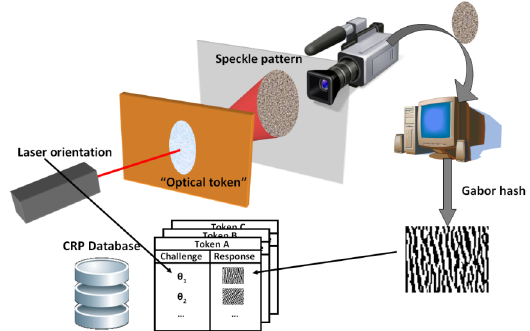
\includegraphics[width=0.8\textwidth]{img/optical-PUF.png}
    \caption{Example of an optical PUF \cite{PUF-study-2010}}
    \label{fig:optical-puf}
\end{figure} 

\subsubsection{Arbiter PUF (A-PUF)}
The idea that delays in integrated circuits (ICs) can be used in PUFs was first introduced by \cite{10.1145/586110.586132}, such PUFs that exploit the delays in ICs are known as Delay-Based PUFs. The specific MUX-chain architecture that defines the Arbiter PUF (A-PUF) as we know it today was later introduced by \cite{9d14141c05ac4f57864d59873ec23799}. The A-PUF is a Delay-Based PUF that exploits the fact that when two electrical signals are launched simultaneously through two identical paths, manufacturing variations will cause one signal to arrive slightly earlier than the other. The A-PUF uses a chain of $n$ multiplexers (MUX) stages, where each stage is controlled by the $n$-th bit of the challenge which determines whether the two signals are crossed over or pass straight through. Due to unavoidable manufacturing differences, the two paths accumulate slightly different delays and an arbiter at the end, typically a D flip-flop, measures which signal arrived first and accordingly produces a response bit of 1 or 0. As seen in figure \ref{fig:A-PUF}, an A-PUF with 128 stages has 128 input bits, which means it has $2^{128}$ possible challenges, as such the A-PUF is considered a strong PUF. However, the additive nature of the delay model that gives the A-PUF its large CRP space also constitutes its primary vulnerability. \cite{10.1145/1866307.1866335} demonstrated that the input-output behavior of the A-PUF can be modeled using logistic regression. For a 64-bit A-PUF, 95\% prediction rate is achieved with as few as 640 CRPs in 0.01 seconds of training time, and 99.9\% accuracy with 18.050 CRPs in under one second of training. This disqualifies the A-PUF for usage in security protocols since it is predictable given enough CRPs.

\begin{figure}[ht!]
    \centering
    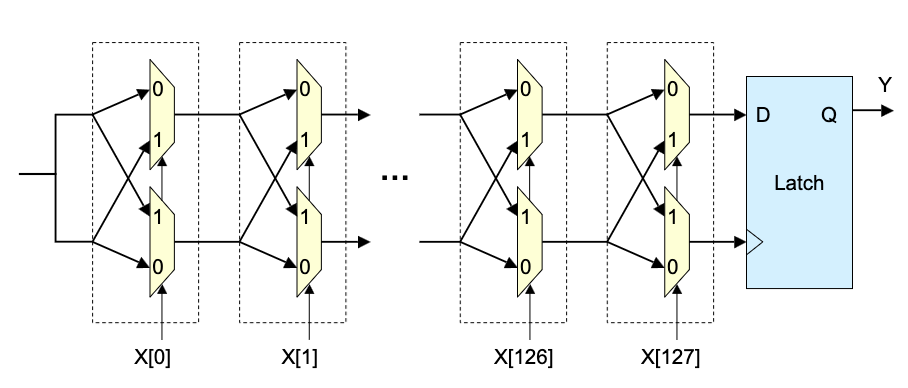
\includegraphics[width=0.8\textwidth]{img/a-PUF.png}
    \caption{Arbiter PUF circuit \cite{10.1145/1278480.1278484}}
    \label{fig:A-PUF}
\end{figure} 

\subsubsection{Ring Oscillator PUF (RO-PUF)}
Initially introduced by \cite{10.1145/1278480.1278484}, the Ring Oscillator PUF (RO-PUF) is a Delay-Based PUF that derives its uniqueness from the differences in oscillation frequencies of multiple identical ring oscillators. Ring oscillators are closed loops of an odd number of inverters whose frequency is determined by the propagation delay of their gates. As seen in figure \ref{fig:RO-PUF}, to generate a sequence of output bits, a fixed sequence of oscillators pairs is selected using the challenge input, and each pair's two frequencies are compared to generate an output bit. Since all the oscillators are identical in design, any frequency difference between them is attributed entirely to manufacturing variations, making the responses unique per device. As mentioned by \cite{10.1145/1278480.1278484}, given $N$ ring oscillators, there are $\frac{N(N/2)}{2}$ distinct pair comparisons. However, the number of truly independent bits is lower than that because the pairwise comparison results are correlated with one another: if oscillator $A$ is faster than $B$, and $B$ is faster than $C$, the outcome of comparing $A$ with $C$ is already implied and contributes no new information. To guarantee fully independent output bits, we can pair each oscillator with exactly one other oscillator, this would yield $N/2$ fully independent response bits for $N$ oscillators, we get fully independent response bits at the cost of requiring more oscillator instances on the PUF. The RO-PUF is therefore considered a weak PUF since its CRP space grows polynomially with the number of oscillators.

\begin{figure}[ht!]
    \centering
    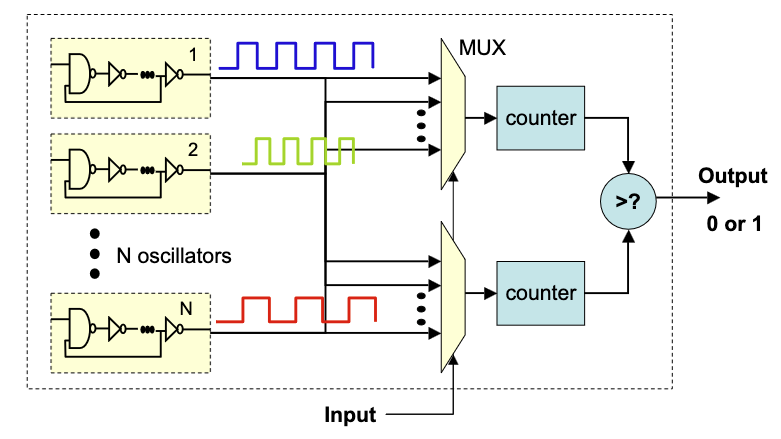
\includegraphics[width=0.8\textwidth]{img/RO-PUF.png}
    \caption{Ring Oscillator PUF circuit \cite{10.1145/1278480.1278484}}
    \label{fig:RO-PUF}
\end{figure} 

\subsubsection{SRAM PUF}
First introduced by \cite{Holcomb2007InitialSS}, the SRAM PUF is a Memory-Based PUF that exploits the random power-up behavior of Static Random Access Memory (SRAM) cells, each of which uses a positive feedback loop to settle into and maintain one of two stable states representing either a 0 or a 1. As seen in figure \ref{fig:SRAM-PUF}, the $V_{th}$ differences in the transistors cause the SRAM cell to start as either 0 (when $A=0, B=1$) or 1 (when $A=1, B=0$) when first powered on. Under normal operations, a write operation forces the cell into one of these states. However, when the SRAM is powered on initially without a preceding write operation, the cell briefly goes into a metastable state in which, theoretically, the feedbacks driving it toward 1 and 0 are perfectly balanced, but in practice, small threshold voltage mismatches between the transistors cause one feedback loop to be slightly stronger than the other, thereby making the cells produce either a 1 or 0. These differences are unavoidable and introduced by the manufacturing process. When the two feedback loops are nearly equal in strength, environmental fluctuations can cause a cell to deviate from its normal state, which results in a bit flip. Error correction is therefore necessary for reliable response generation. The key recognition which allows SRAM PUFs to easily be error corrected is the fact that any cell that is biased towards 0 or 1 will remain strongly biased toward its starting state. Therefore, through repeated measurements, we can assess the stability of each cell and only use the most stable cells for key generation. Although in practice, we also need to use error-correcting codes along with the initial filtering for reliable and reproducible responses. The SRAM PUF is a weak PUF since we get as many output bits as we have cells. The challenge can be which SRAM cell addresses to read or simply the entire SRAM.

\begin{figure}[ht!]
    \centering
    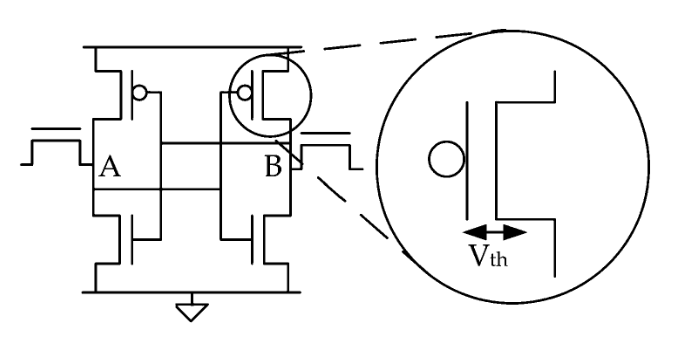
\includegraphics[width=0.8\textwidth]{img/SRAM-PUF.png}
    \caption{SRAM cell \cite{6823677}}
    \label{fig:SRAM-PUF}
\end{figure} 


\subsection{PUF Threats and Attacks}
While PUFs offer interesting security properties by deriving secrets from uncontrollable manufacturing variations, they are not immune to attacks. The security depends heavily on the PUF architecture used and the capabilities of the adversary. Previous research has identified and demonstrated  several classes of attacks that can compromise PUF security. From machine learning attacks that exploit the structure of the PUF's challenge-response behavior to physical side-channel attacks that bypass the CRP interface by monitoring the unintended emissions of the device, many attacks against PUFs are possible. We will now see some of them.

\subsubsection{Machine Learning / Modeling Attacks}
Machine learning (ML) attacks are the most studied and practically demonstrated threat against PUFs and constitute the primary security concern for strong PUF architectures such as the Arbiter PUF. The adversary is assumed to have temporary access to the PUF, during which they collect a large set of challenge-response pairs by querying the PUF. These CRPs are then used to train a mathematical model that can approximate the behavior of the PUF. After training, the model can predict the PUF's response to previously unseen challenges with very high accuracy. \cite{10.1145/1866307.1866335} demonstrated that a 64-bit Arbiter PUF can be modeled using logistic regression with prediction accuracies of more than 99\% with as few as 10,000 CRPs, while more complex architectures such as XOR Arbiter PUFs, which were initially introduced as a countermeasure to protect Arbiter PUFs against ML attacks, were shown to still be vulnerable to modeling attacks using linear regression, although the number of CRPs and training time required for modeling is significantly higher than what is needed for a simple unprotected Arbiter PUF. For example, modeling a 64-bit XOR Arbiter PUF with 6 XORs requires around 200,000 CRPs and takes 31:01 hours. The fundamental reason for this vulnerability lies in the additive delay model behind the Arbiter PUF's behavior since the responses are determined by a linear function of the challenge bits, which can be learned given enough CRPs. 

\subsubsection{Physical Attacks}
Physical attacks involve direct observation of the PUF as a physical object rather than capturing its CRPs. \cite{6581556} were able to physically clone an SRAM PUF using Focused Ion Beam (FIB) circuit edit. While such physical attacks require very expensive machinery and high expertise, they remain realistic for a sufficiently supported and motivated adversary. The mere existence of such successful physical cloning attacks undermines the foundational security assumption on which PUFs are based, which is that the physical characteristics introduced by the manufacturing process are impossible to replicate.

\subsubsection{Side Channel Attacks}

Side-channel attacks are carried out by observing the physical emissions produced by the device during PUF querying. Simple Power Analysis (SPA) is a technique that measures power consumption while executing some algorithm. Since different operations have different power consumption patterns, one can distinguish an addition operation from a multiplication operation simply by looking at the power consumption patterns. If the algorithm handles some secret data like a key bit by bit and runs different operations based on if the bit is a 0 or a 1, then extracting the key from the power consumption chart is obvious. As seen in figure \ref{fig:SPA}, 1 bits appear as tall bumps and 0 bits as short bumps. However in practice, noise prevents such clear distinction between 1s and 0s. Differential Power Analysis (DPA) is typically used rather than SPA to account for the noisy power consumption patterns. DPA is a statistical method for identifying data-dependent correlations from power consumption \cite{AnySiliconDPA}. 

\begin{figure}[ht!]
    \centering
    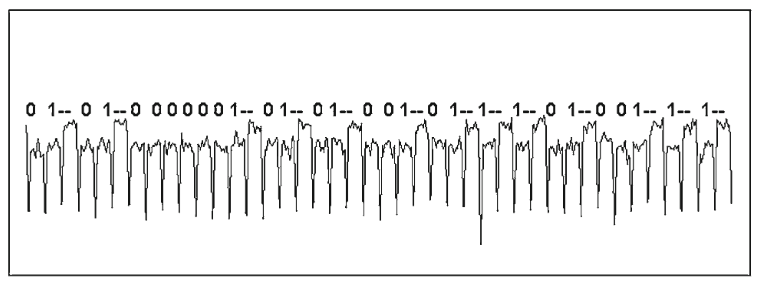
\includegraphics[width=0.8\textwidth]{img/SPA.png}
    \caption{SPA leaks from an RSA implementation \cite{Kocher2011}}
    \label{fig:SPA}
\end{figure} 

The same attacks can also be applied to electromagnetic leakage (EM) since power consumption is proportional to the current demanded by the circuit, and current is just a flow of electrons, and this flow of electrons produces an electromagnetic field which can be measured. One downside of doing power analysis using EM leakage is the fact that the probe must be placed right on top of the area of interest so as not be impacted by the EM radiation from neighboring events (see figure \ref{fig:EM-probe}). Using this principle, \cite{11316252} were able to determine the frequency of one of the ROs involved in one of the challenges of the PUF by measuring EM traces along a grid of points near the FPGA where the RO PUF is implemented. As demonstrated by \cite{10.1007/978-3-642-21599-5_3}, it is also possible to attack the fuzzy extractors, which are used to error-correct the noisy PUF outputs, to extract the generated key.

\begin{figure}[ht!]
    \centering
    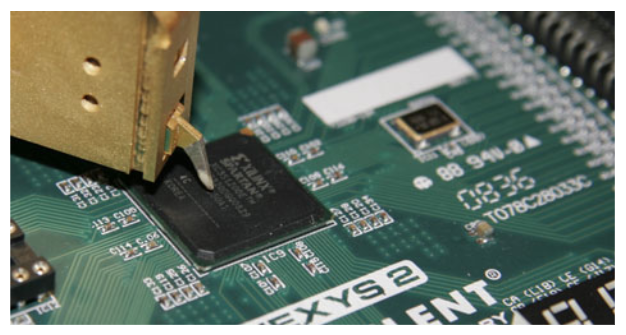
\includegraphics[width=0.5\textwidth]{img/EM-measure.png}
    \caption{EM probe over an FPGA chip \cite{10.1007/978-3-642-21599-5_3}}
    \label{fig:EM-probe}
\end{figure} 


\subsection{Error Correction and Fuzzy Extractors}
Since PUF responses are noisy due to environmental variations, they cannot be used directly as cryptographic keys. Initially introduced by \cite{Dodis_2008}, Fuzzy Extractors are a cryptographic tool for generating a stable secret key from a noisy source such as PUF responses or biometric measurements. A fuzzy extractor consists of two procedures: \textbf{Generate} (Gen) and \textbf{Reproduce} (Rep). As seen in figure \ref{fig:fuzzy}, The Gen function takes a noisy input $w$ and generates a secret key $R$ and public helper data $P$. In a subsequent measurement, we get a noisy input $w'$, the Rep function takes $w'$ and the public helper data $P$ and reproduces the secret key $R$.

The code-offset method shown by \cite{Maes_2016} is an example of how a Fuzzy Extractor can be used to generate a key from a PUF response. As seen in figure \ref{fig:code-offset}, a PUF-based key generator has two phases: Enrollment and reconstruction. The following happens during enrollment:
\begin{enumerate}
    \item A random number generator (RNG) generates a random seed $S$.
    \item A key derivation function (KDF) generates a secret key $K$ using the seed $S$.
    \item The seed $S$ is encoded using an error-correcting code to produce a code word $C$.
    \item The PUF is queried to produce a response $X$.
    \item The response $X$ is XORed with the code word $C$ to produce helper data $W$
    \item The helper data $W$ is stored publicly and the key $K$ is enrolled; enrollment of the key means that we associate its identity with some helper data $W$ and some challenge $C$ that produced the response $X$. After enrollment the key can be discarded since we can reconstruct it in the reconstruction phase.
\end{enumerate}
The reconstruction phase does the following:
\begin{enumerate}
    \item To reconstruct the enrolled key $K$, we first query the PUF to get the noisy response $X'$ using the same previous challenge $C$.
    \item The helper data $W$ associated with the key $K$ is then XORed with the noisy response to produce a noisy code word $C'$.
    \item The noisy code word $C'$ is decoded using the same error correction code used to encode it.
    \item The decoded seed $S'$ is given to the KDF to generate the reconstructed key $K'$.
    \item If the subsequent noisy PUF response $X'$ is close enough to the original response $X$, then the keys $K$ and $K'$ will be identical.
\end{enumerate}

The success of the reconstruction phase depends on whether the noisy PUF response $X'$ is sufficiently close to the original response $X$. If the number of flipped bits exceeds the error correction capability $t$ of the chosen error-correction code, the decoder will produce an incorrect seed $S'$, resulting in a different key $K'$. However, the usage of public helper data is not without flaws. \cite{6965637} demonstrated that attackers could use the public data to infer information about the PUF's response and also manipulate said helper data to recover the secret key by observing system failure rates.


\begin{figure}[ht!]
    \centering
    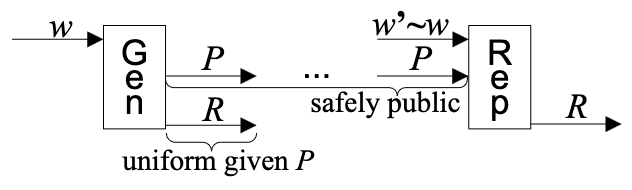
\includegraphics[width=0.8\textwidth]{img/fuzzy-extractor.png}
    \caption{Fuzzy extractor \cite{Dodis_2008}}
    \label{fig:fuzzy}
\end{figure} 


\begin{figure}[ht!]
    \centering
    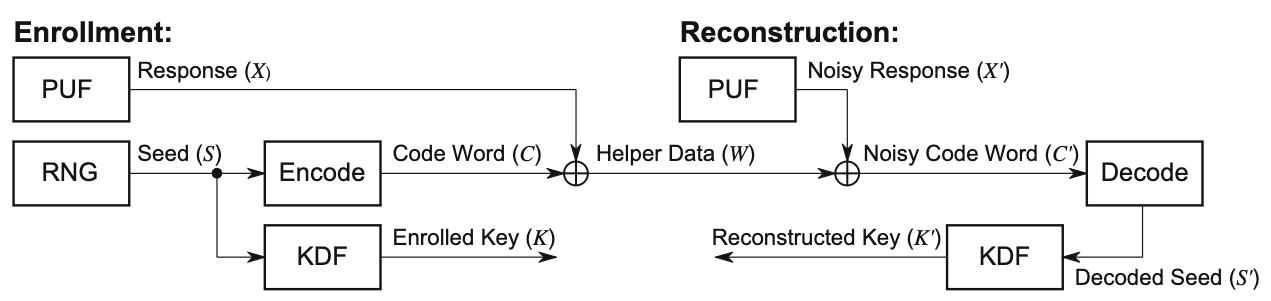
\includegraphics[width=1\textwidth]{img/code-offset.png}
    \caption{PUF-based key generator based on the code-offset method \cite{Maes_2016}}
    \label{fig:code-offset}
\end{figure} 


\subsection{Applications of PUFs}
% Find examples in https://dl.acm.org/doi/epdf/10.1145/3487060
\subsubsection{Device Authentication}
%with CRP DB: https://ieeexplore.ieee.org/abstract/document/7424628
%without CRP DB: https://www.acsu.buffalo.edu/~mblanton/cse708/pufs-without-database.pdf
One of the most researched applications of PUFs is device authentication. For strong PUFs, the most basic form of PUF-based authentication can be achieved using a database of prerecorded CRPs \cite{10.1145/3487060}. As seen in figure \ref{fig:CRP-DB-Auth}, a device / prover $p$ authenticates with a server / verifier $v$. The protocol has two phases, the enrollment phase (Phase 1) and the authentication phase (Phase 2). During the enrollment phase, the device is enrolled into a database by recording some of its CRPs, this step would be carried out by the manufacturer or organization before distributing the devices. At the end of this phase, each device $d_{id}$ will have a set of its CRPs stored in the database $\Gamma_{id} = \{(c_0, r_0), \dots, (c_n, r_n)\}$. In the authentication phase, the verifier $v$ selects some challenge $c'_i$ associated with the device and sends it to the device. Once the device receives the challenge $c'_i$, the PUF is queried to produce the response $r''_i = \Psi_p(c'_i)$, then the device sends the response $r''_i$ to the verifier. If the received response is identical or close enough to the one recorded in the CRP database ($r''_i \simeq r'_i$), then the device is authenticated, otherwise authentication fails. For higher security, CRPs are only used once to prevent replay attacks. While this challenge-response protocol approach is ideal for strong PUFs that have a large CRP space where we can afford only using a CRP once, weak PUFs cannot be used as efficiently and securely with this protocol. 
\begin{figure}[ht!]
    \centering
    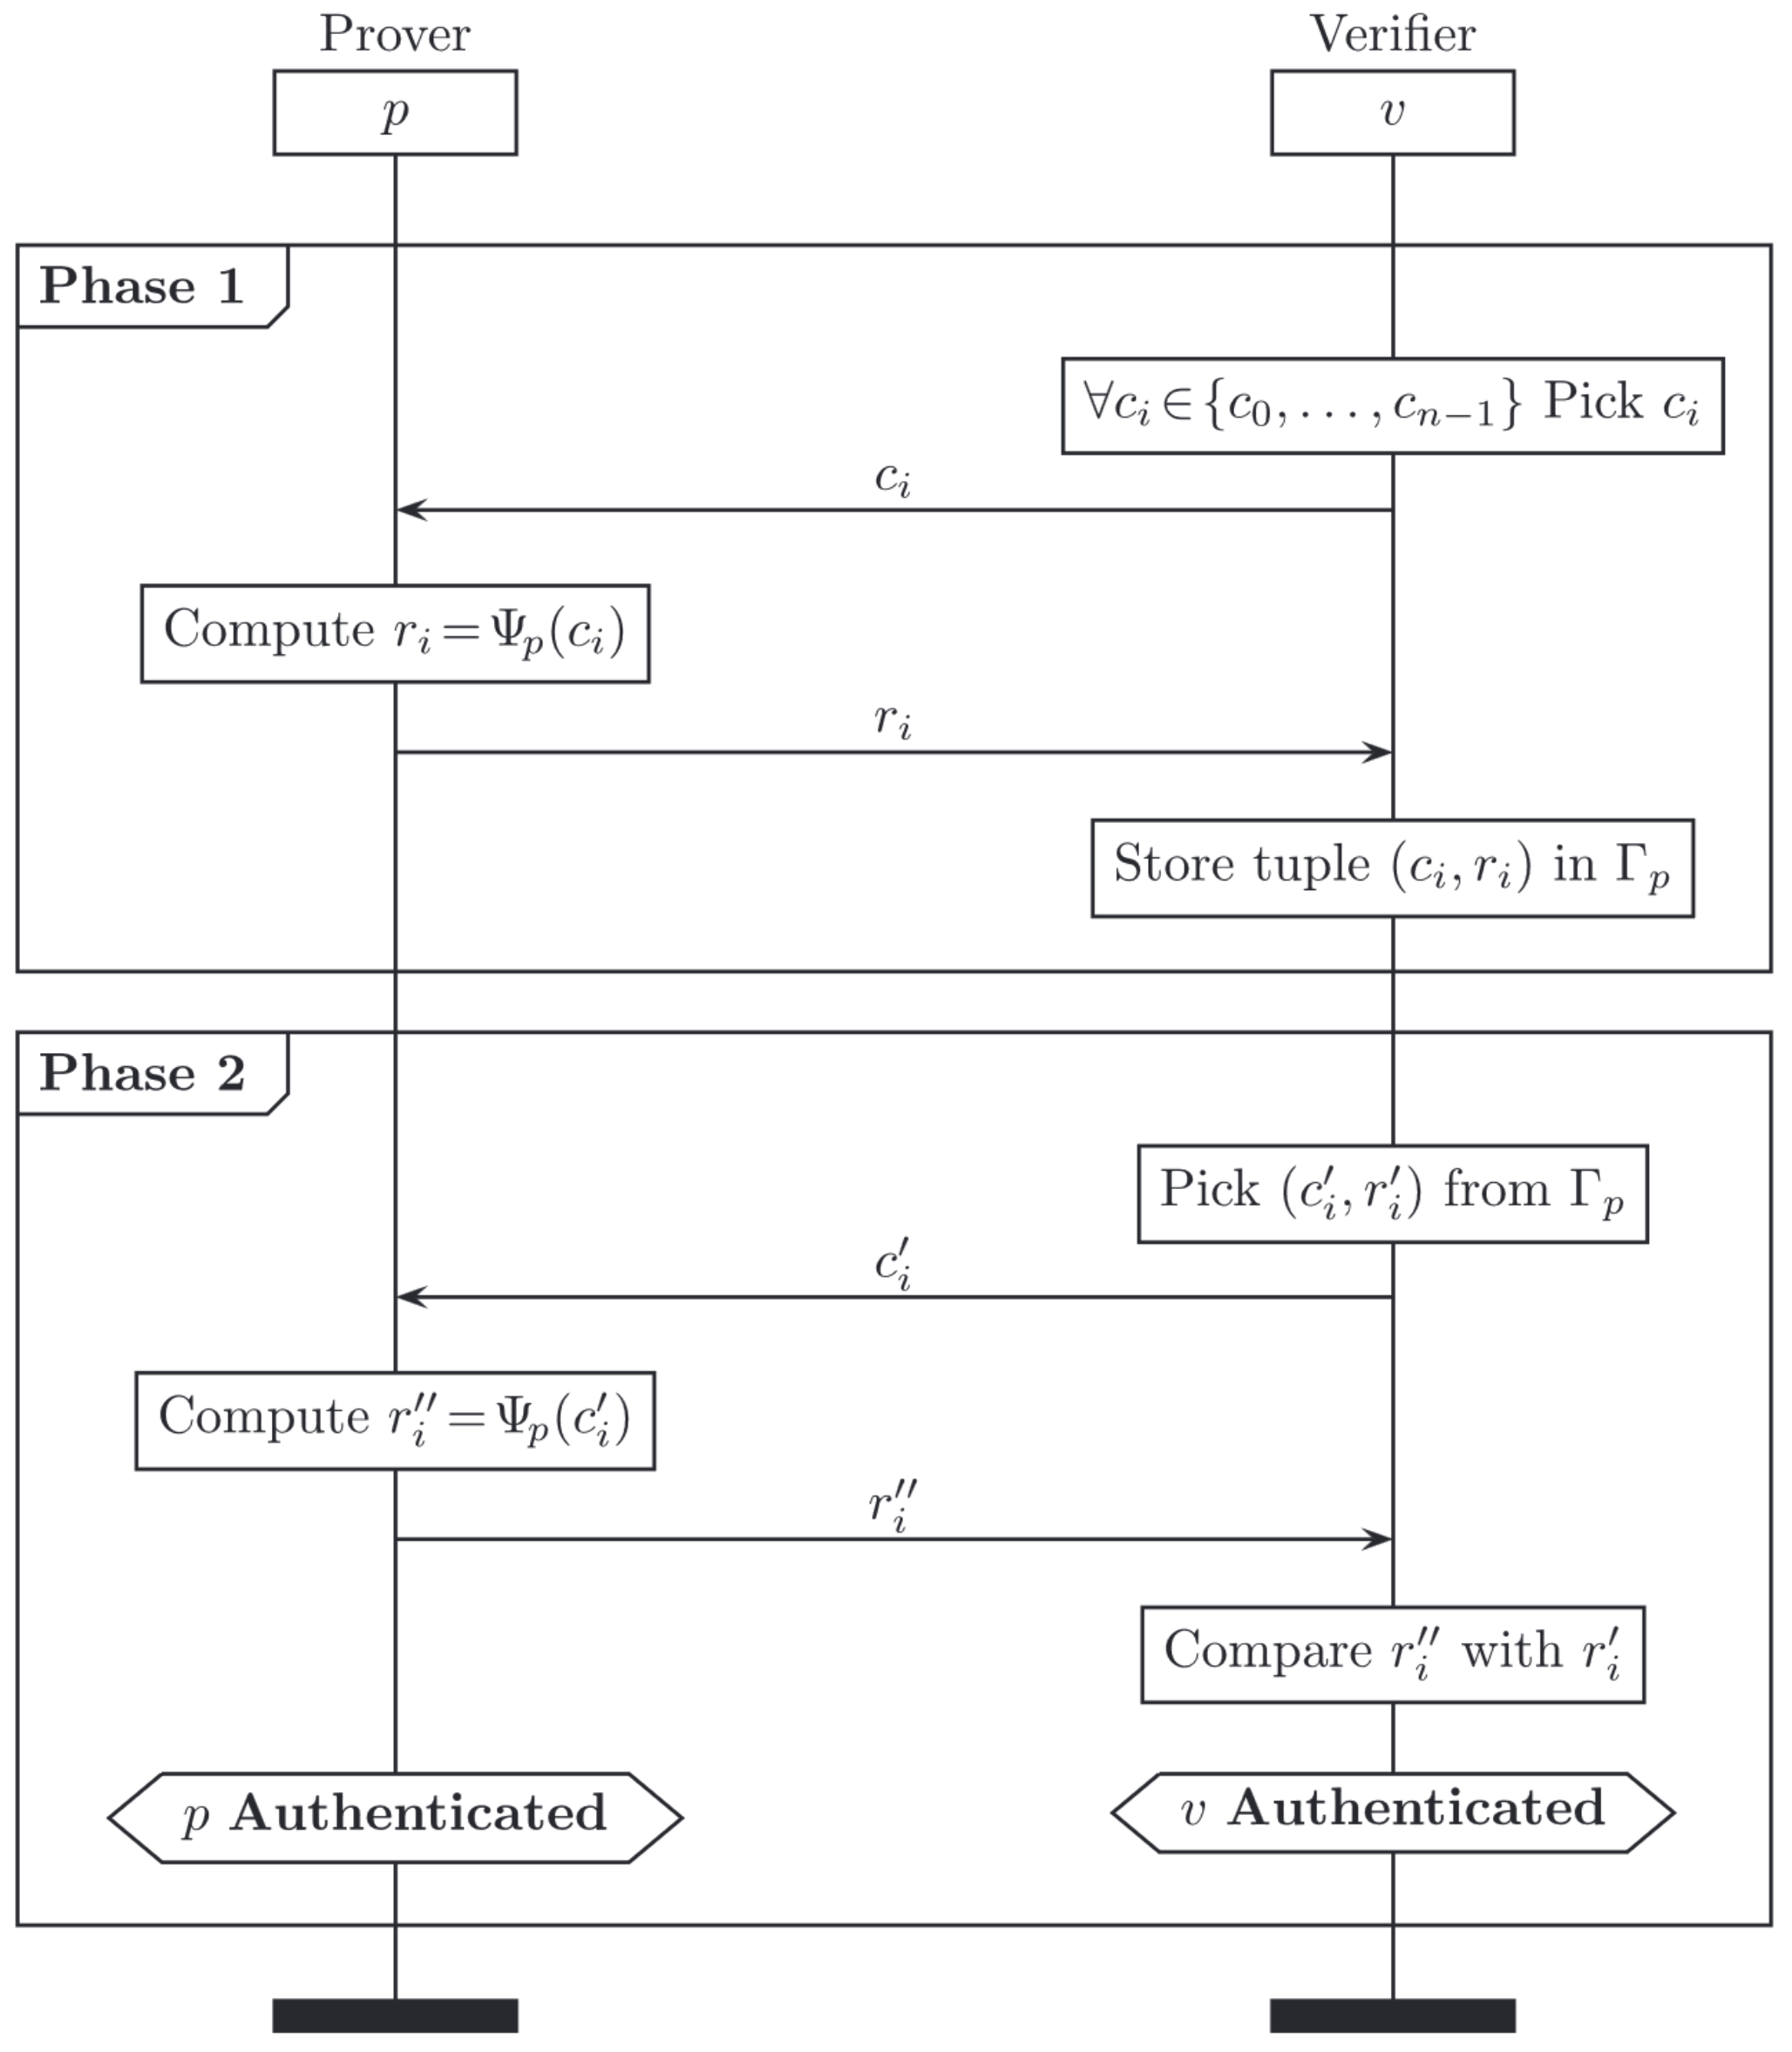
\includegraphics[width=0.7\textwidth]{img/CRP-DB-Auth.png}
    \caption{PUF-based authentication using prerecorded CRPs \cite{10.1145/3487060}}
    \label{fig:CRP-DB-Auth}
\end{figure} 

To achieve authentication, weak PUFs like the SRAM PUF are used as primitives for cryptographic keys or in a similar fashion. As shown by \cite{9233424} on figure \ref{fig:SRAM-Auth}, a fingerprint can be extracted from the SRAM PUF during enrollment and saved, then to authenticate the device, the server sends a nonce and challenge, the device gets the fingerprint from the its SRAM PUF, then to augment the weak PUF, its output $PUF$ is reordered using a challenge to produce $RPUF$, then the response of this authentication request is the hash $H(nonce \space \oplus \space RPUF \space \oplus \space PUF)$, the hash is sent as a response to the server which can in turn verify if the received response matches the expected response. The fingerprint here is a stable construct generated by identifying the most stable bits in the SRAM PUF to only use those that have a stability of 100\%, and an ECC algorithm is used to generate helper data for error correction.
As we can see, when a weak PUF is used in authentication, the device is not required to send its raw PUF responses anymore, but rather the output of the PUF is used to "sign" some nonce to prove to the server that the PUF is there.
\begin{figure}[ht!]
    \centering
    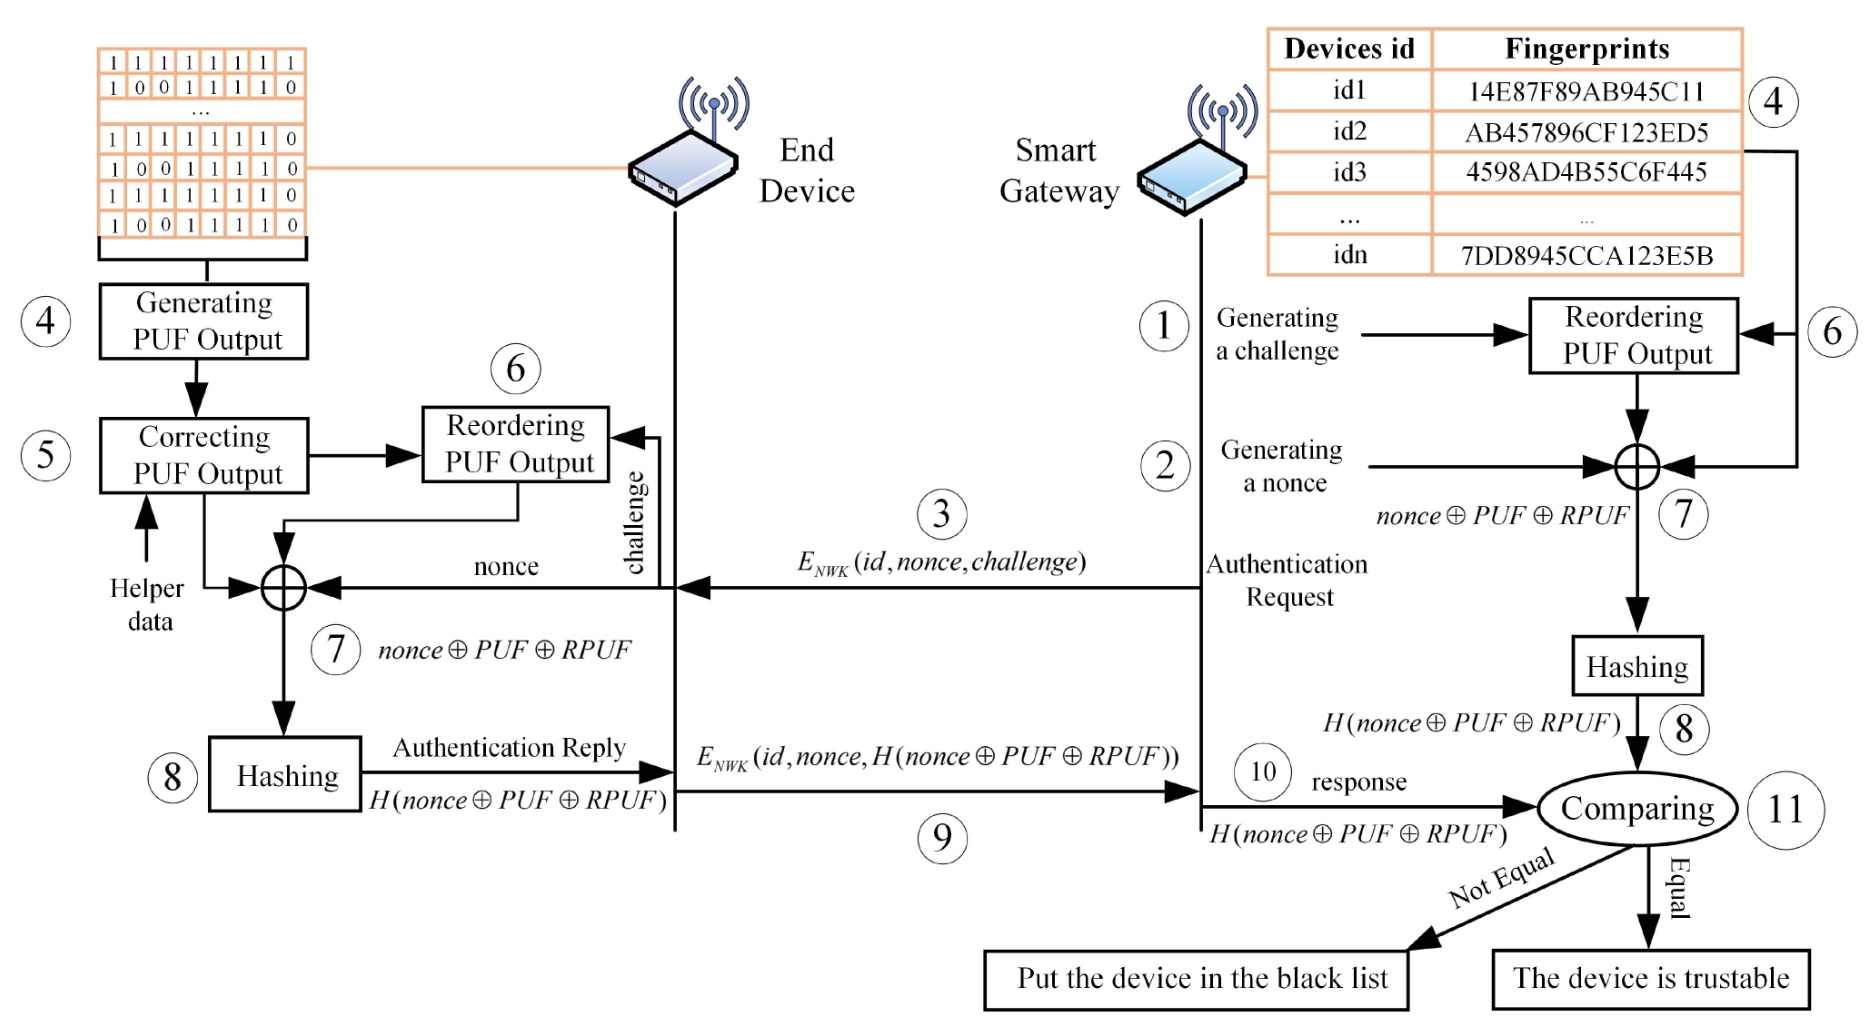
\includegraphics[width=\textwidth]{img/SRAM-Auth.png}
    \caption{Example of PUF-based authentication using a weak PUF \cite{9233424}}
    \label{fig:SRAM-Auth}
\end{figure} 

\subsubsection{IP Protection}
PUFs can be used for hardware intellectual property (HW-IP) protection of FPGA design. The bit-stream used to program the FPGA usually lives on some sort of non-protected flash memory. When the FPGA is powered on, the bit-stream is loaded onto the FPGA to configure it. During this loading phase, an attacker can easily tap into the wires between the flash memory and the FPGA to copy the bit-stream. If this bit-stream is illegally copied, it can lead to revenue loss since using such IP requires licensing. PUFs are used in this context to generate the keys which encrypt this bit-stream when stored in flash memory, then when the FPGA chip receives the encrypted bit-stream, it uses an internal PUF implemented within the FPGA chip to derive a key to decrypt the bit-stream and configure the FPGA, as shown by \cite{4380646}.

\subsubsection{Secure Boot}
Secure boot is a mechanism that ensures a device only executes authorized and unmodified firmware at startup to protect against attacks where the legitimate firmware is replaced with malicious firmware before the device powers on. PUFs can be used as hardware root of trust for a secure boot. As mentioned by \cite{SecureBootPUF2024}, classical secure boot approaches often rely on one public key used by all devices to verify integrity, if its private key is compromised then all devices are compromised. PUFs eliminate this problem entirely by deriving one unique key per device with no key ever getting stored on the device. As such, \cite{SecureBootPUF2024} proposed a PUF-based secure boot mechanism for RISC-V architecture in which the secure element retrieves a boot key from the PUF using a boot challenge stored in one-time programmable memory.

\subsubsection{Random Number Generation}
Beyond key generation and authentication, PUFs can also serve as a source of true random numbers, which are essential for generating nonces, session keys, and initialization vectors. For example, the same random settling of bistable cells at power up that makes SRAM cells useful as a PUF can be exploited as a source of entropy for random number generation. The SRAM cells where the two feedback loops are equal in strength are more susceptible to random noise and therefore settle unpredictably, making them a good source of randomness. \cite{4674345} made this observation and developed the FERNS method (Fingerprint Extraction and Random Numbers in SRAM). At power-up, 0-skewed or 1-skewed cells will power-up to 0 or 1 respectively regardless of the noise conditions in most cases (light cells with low entropy in figure \ref{fig:SRAM-Rand}), such cells will form the basis of the fingerprinting to provide identification. Whereas neutral-skewed cells, that do not have a strong tendency toward either state can powerup to either 0 or 1 (dark cells with high entropy in figure \ref{fig:SRAM-Rand}), will provide randomness, making the SRAM serve as both a PUF and a TRNG. As such, they demonstrated that a 512-byte SRAM fingerprint contains sufficient entropy to generate 128-bit true random numbers and that the generated numbers pass the NIST randomness tests. One limitation of this approach is that the entropy is only generated during power-up, which is less practical than a dedicated TRNG circuit that can be queried at any time, but it comes with the advantage that no extra circuit is needed.

\begin{figure}[ht!]
    \centering
    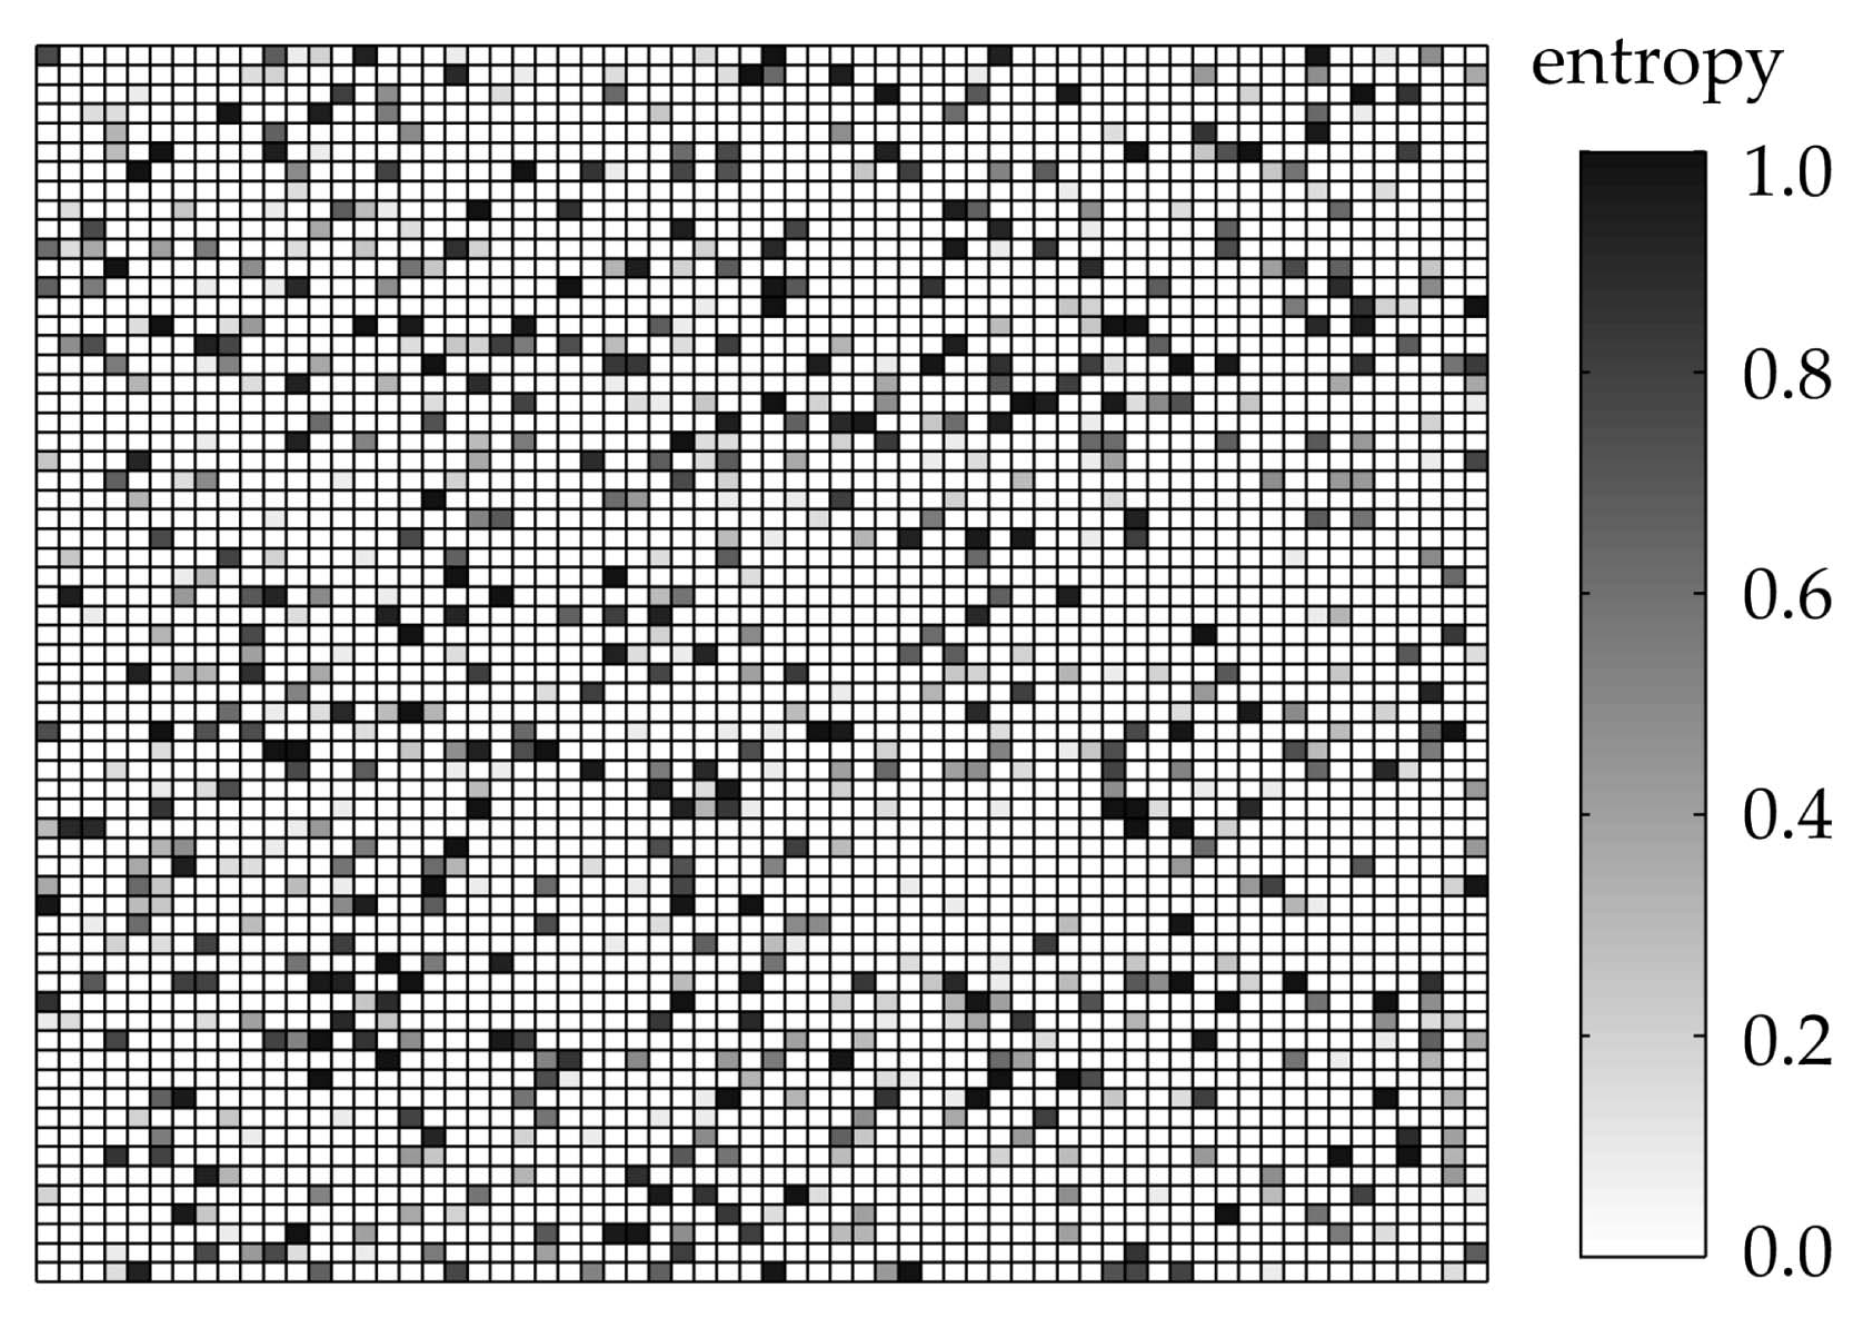
\includegraphics[width=0.8\textwidth]{img/SRAM-Rand.png}
    \caption{SRAM cells entropy determined from 100 power-ups at 294 K. \cite{4674345}}
    \label{fig:SRAM-Rand}
\end{figure} 

\section{CHOICE PUF}

The CHOICE PUF introduced by \cite{9556423} is a delay-based weak PUF or more accurately a delay-tunable PUF. Indeed, its main novelty is the fact that it is tunable, meaning that by changing the challenges a certain way, it is possible to increase or decrease the probability of obtaining 1s in the PUF response. This tuning property also allows us to find at least one challenge per FPGA board type that has the lowest bit-error rate (BER) and ideal uniqueness and uniformity. Although the authors claim that the CHOICE PUF has a low footprint on the FPGA, our testing of their implementation on other boards showed that the CHOICE PUF takes a considerable amount of FPGA slices since each PUF cell needs four 32-bit addressable shift registers (ASRs). In this section, we will explain the inner workings of the CHOICE PUF. This PUF architecture warrants its own section because it is the PUF we used for the REPUSH protocol implementation.

\subsection{Addressable Shift Register (ASR)}
To understand the CHOICE PUF architecture, we must first understand how ASRs operate. ASRs are sequential logic circuits that can be used to store serial data. As seen in figure \ref{fig:ASR}, an ASR is a chain of D flip-flops with a multiplexer at the end. A D flip-flop (D-FF) captures the value present at its data input \verb|D| on an active clock signal (\verb|CE=1| and rising \verb|clk| edge) and holds that captured value as its output \verb|Q| until the next active clock signal which can change its content again based on what the data input is, thereby acting as a single-bit memory. In the ASR, $S$ number of such flip-flops ($q_0, q_1, \dots,q_{S-1}$) are connected in series such that the output of each stage feeds the data input of the next, and on each active clock edge (gated by signal \verb|ce|), the input signal \verb|d| is captured into the flip-flop $q_0$ while every subsequent flip-flop captures the value of its predecessor, propagating the data one stage forward through the chain. The ASR exposes the output of each of its flip-flops through a multiplexer (MUX) which accepts as input an address $a$ as a bus of length $\log_2(S)$, the address $a$ is an integer in binary format which determines which flip-flop's output to read out into the MUX's output \verb|Q|. A selected flip-flop $q_i$ will propagate to the MUX with some delay $\tau_i$ since the wires leading from the flip-flops to the MUX are of variable lengths, as we will see later, the CHOICE PUF exploits this fact as part of its delay model. 
\begin{figure}[ht!]
    \centering
    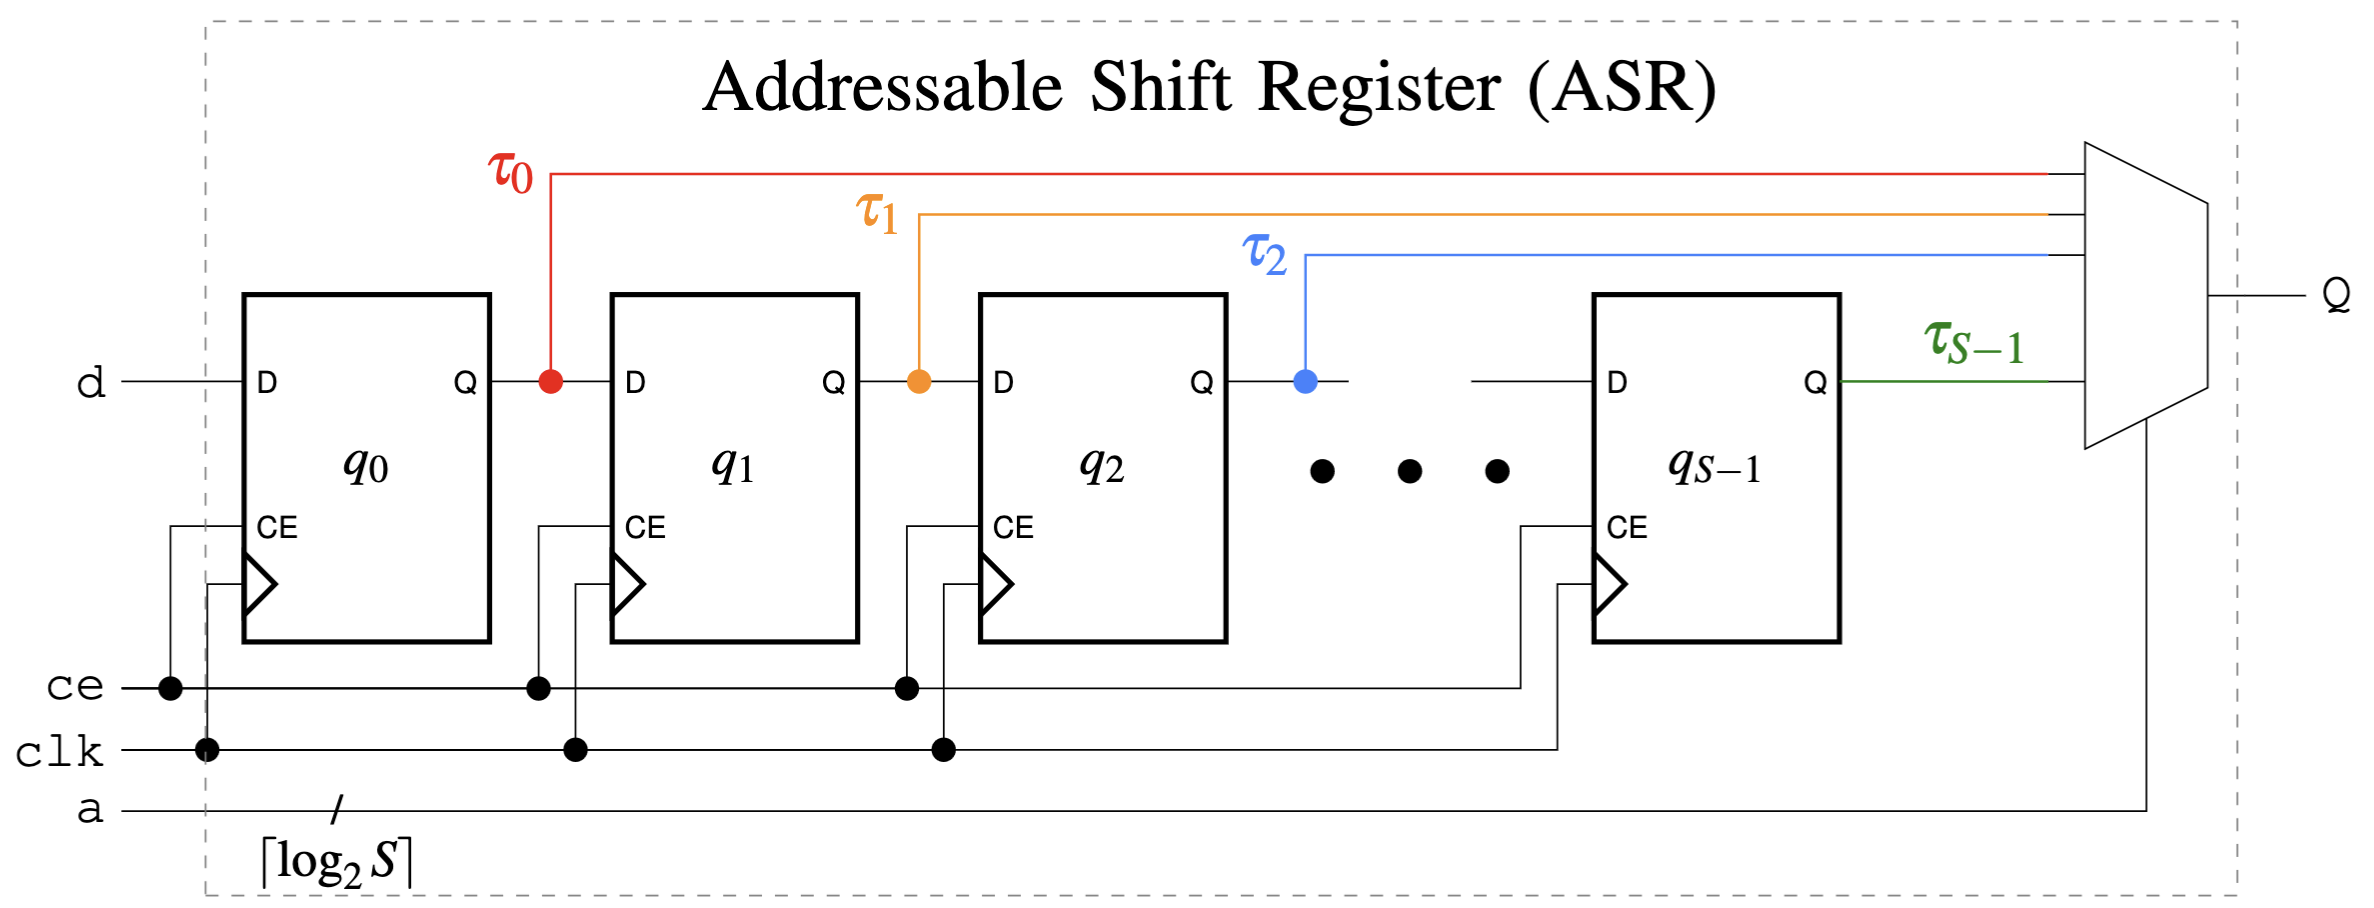
\includegraphics[width=\textwidth]{img/ASR.png}
    \caption{S-stage Addressable Shift Register (ASR). \cite{9556423}}
    \label{fig:ASR}
\end{figure} 
\subsection{PUF Architecture}
As seen in figure \ref{fig:CHOICE-PUF}, a CHOICE PUF cell consists of four 32-bit ASRs ($ASR_0, \dots, ASR_3$) where each ASR controls one corresponding MUX ($MUX_0,\dots,MUX_3$). The output of $o_{MUX_0}$ of multiplexer $MUX_0$ controls the asynchronous set input \verb|PRE| of a flip-flop which will store the PUF output bit, the \verb|PRE| input essentially just makes the flip-flop store something independent of the clock cycle. Each $ASR_i$ can be adjusted via its address input $a_i$ to influence the ASR's propagation delay $\tau_{ASR_i}$, since as we have seen before, inside the ASR, the wires leading to the final multiplexer are of different lengths and thus of different delays. The propagation delay $\tau_{ASR_i}$ is the delay between a change of the output of the ASR's selected internal flip-flop that is selected by address $a_i$ and the occurrence of the signal at the $MUX_i$. Each $MUX_i$ has a logic 0 signal at its 0 position and the output $o_{MUX_{i+1}}$ as its 1 position, except $MUX_3$ which always has a logic 1 signal at its 1 position.    

\begin{figure}[ht!]
    \centering
    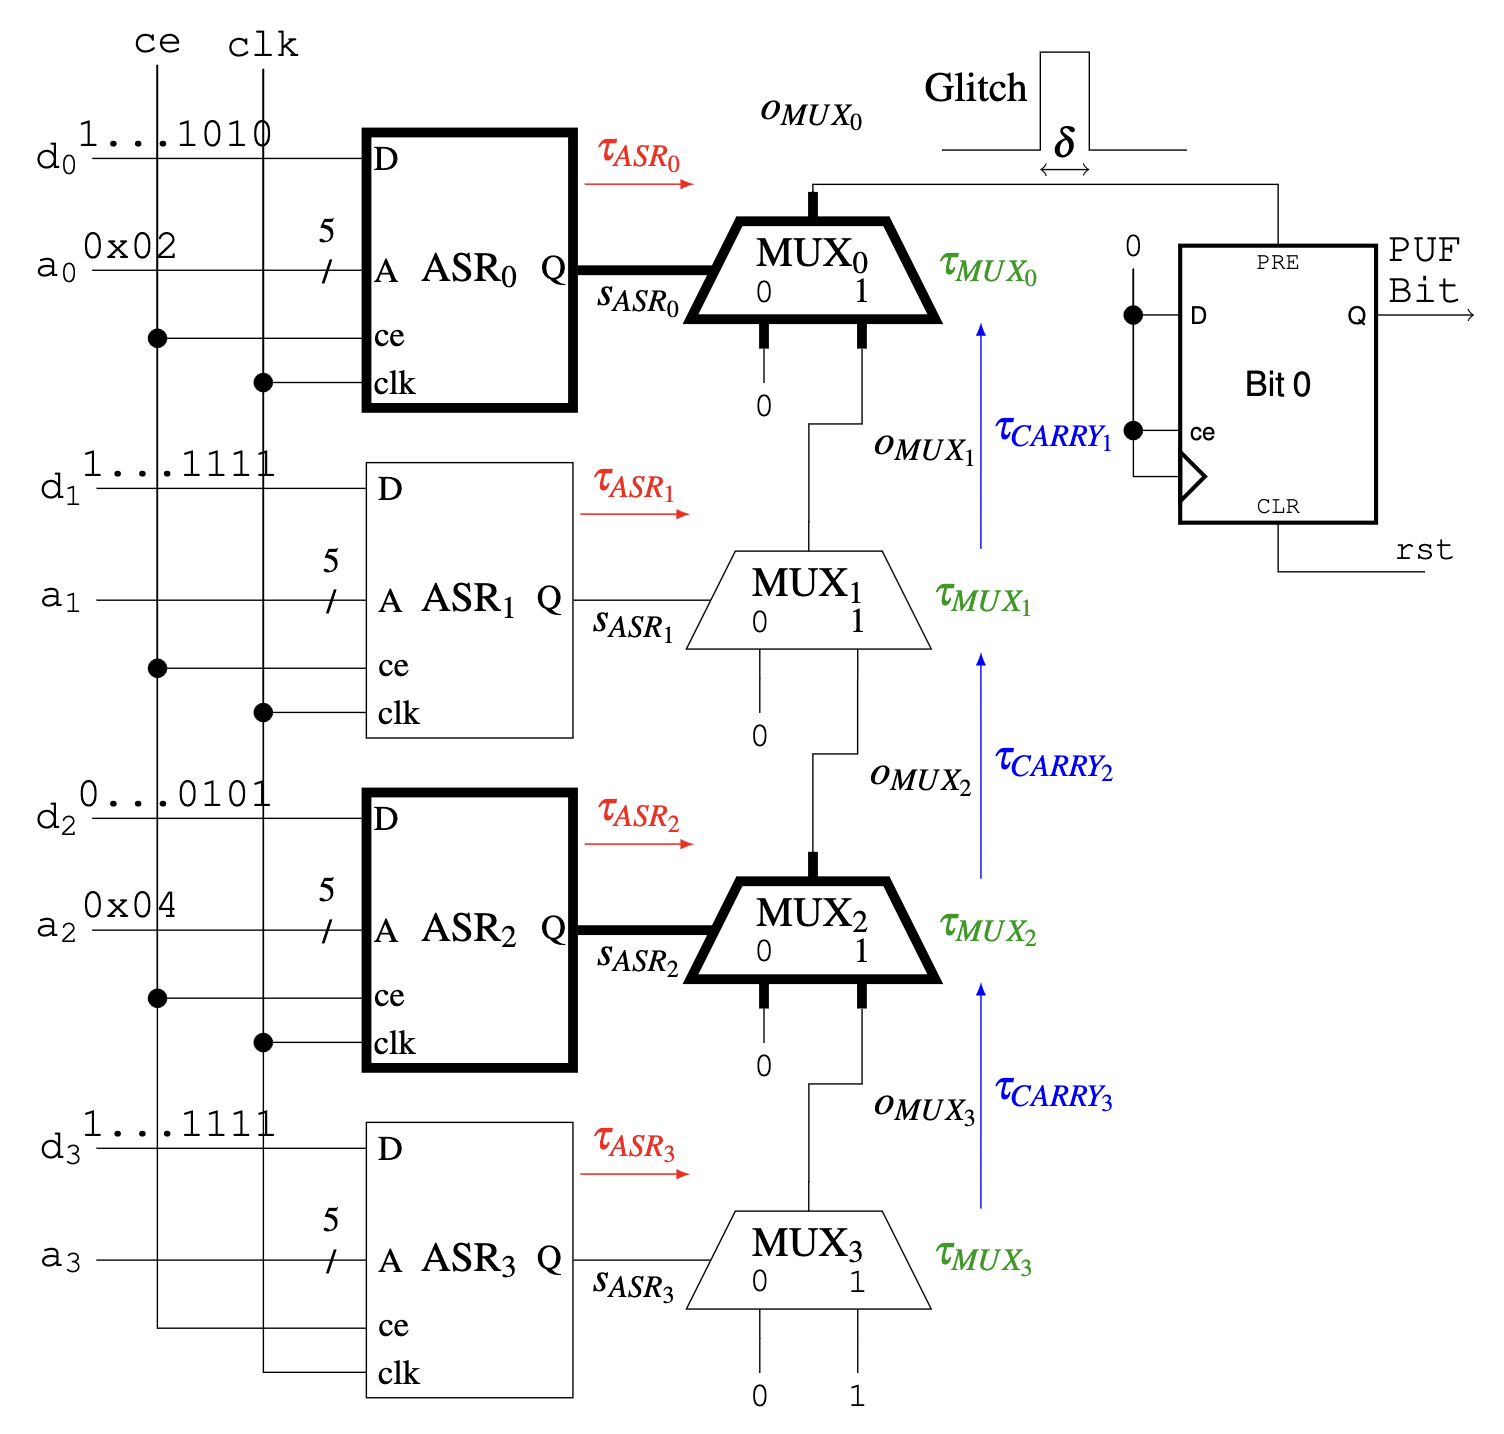
\includegraphics[width=\textwidth]{img/CHOICE-PUF.png}
    \caption{CHOICE PUF cell circuit. \cite{9556423}}
    \label{fig:CHOICE-PUF}
\end{figure}

As part of the PUF challenge, only two of the four ASRs are selected for generating a glitch at $o_{MUX_0}$ (ASRs with a bold outline in the figure \ref{fig:CHOICE-PUF}). The first active ASR will be referred to as $ASR_i$ and the second as $ASR_j$ where $i < j$ and $i,j\in\{0,1,2,3\}$. The two remaining ASRs are considered as inactive since clock cycles will not toggle any signal change on their outputs because they are initialized as all 1s. It is possible to select $\binom{4}{2}=6$ pairs of ASRs as active as part of the PUF challenge. The chosen addresses $a_i$ and $a_j$ of the respective selected ASRs $ASR_i$ and $ASR_j$ are also part of the PUF challenge. As such, we get a total of $\binom{4}{2}\cdot32^2 = 6144$ possible PUF challenges. Each challenge can be defined as a tuple $C=(i,j,a_i,a_j)$. To cause a glitch (small burst of a logic 1 signal) at $o_{MUX_0}$, each ASR must be set with a specific bit pattern $P(k)$ depending on its position $k$ in the PUF cell, as shown in equation \ref{eq:Pk}. Inactive ASRs ($k \notin \{i,j\}$) are initialized with a sequence of all 1s, while $ASR_i$ is initialized either with $1\dots1010$ if $a_i$ is an even address or $0\dots1010$ if $a_i$ is odd. In contrast, $ASR_j$ is initialized with $0\dots0101$ if $a_j$ is even or $1\dots1010$ if $a_j$ is odd.
\begin{equation}
P(k) =
\begin{cases}
1\dots1111 & \text{if } \space k \notin \{i,j\} \\
1\dots1010  & \text{else if } \space k = i \space \land \space a_k\bmod2 = 0 \\
1\dots1010  & \text{else if } \space k = j \space \land \space a_k\bmod2 \neq 0 \\
0\dots0101 & \text{else}
\end{cases}
\label{eq:Pk}
\end{equation}

To get $N$ PUF bits as output, we simply instantiate $N$ PUF cells where we apply the same challenge tuple $C=(i,j,a_i,a_j)$.
\subsection{Querying}
The CHOICE PUF is queried in the following phases:
\begin{enumerate}
    \item Fill (31 cycles): all ASRs are driven bit by bit to fill them with their respective bit patterns $P(k) = d_k$. For the two active ASRs, only the last 31 bits ($d_k[1\ldots31]$) of the bit pattern are initially loaded. The two addresses $a_i$ and $a_j$ are also set during this phase.
    \item Reset: For each PUF cell, the output flip-flop is cleared.
    \item Measurement (1 cycle): For the two active ASRs, \verb|ce| is activated and the first bit $d_i[0]$ of the pattern is driven into the ASRs at the same time to trigger the race.
    \item Settling (2 cycle): We wait for the race to resolve.
    \item Readout: The output flip-flop's bit is captured as the PUF cell's response. 
\end{enumerate}

\subsection{Delay Model}
Whether a PUF cell outputs a 1 or 0 at the end depends on the width $\delta$ of the glitch at $o_{MUX_0}$. The output flip-flop has a minimal glitch width $\delta_{min}$ that is required to successfully drive the \verb|PRE| input and set it to 1 as seen in equation \ref{eq:puf-out-delta}. This minimal glitch width $\delta_{min}$ depends on the resistive and capacitive load (RC) of the routing path from $o_{MUX_0}$ to the output flip-flop since the path acts as a low-pass filter which will ignore glitches that are not wide enough. 

\begin{equation}
PUF =
\begin{cases}
1 & \delta \ge \delta_{min} \\
0 & \delta < \delta_{min} 
\end{cases}
\label{eq:puf-out-delta}
\end{equation}

We shall now derive a formula for the glitch width $\delta$ based on the delays of the PUF cell. For the two selected ASRs, let us consider the delays $\tau_i=\tau_{ASR_i} + \tau_{MUX_i}$ and $\tau_j=\tau_{ASR_j} + \tau_{MUX_j}$, where $\tau_{ASR_k}$ is a delay determined by the chosen address $a_k$ of the ASR and $\tau_{MUX_k}$ is the delay introduced by the routing inside the multiplexer. We also consider $\tau_{CARRY_k}$ as the time required to forward a signal from the output $o_{MUX_k}$ of a multiplexer to the 1-data input of the $MUX_{k-1}$ above it on the carry chain. The delay between the output of $MUX_j$ and the output of $MUX_i$ can be written as:
\[ \tau_{i,j} = \sum_{k=i}^{j-1}\tau_{CARRY_{k+1}}+\tau_{MUX_k} \]
With these definitions of $\tau_i$, $\tau_j$ and $\tau_{i,j}$, there exists three different delay scenarios that would determine the glitch width $\delta$, as seen in figure \ref{fig:CHOICE-PUF-Delay}.
\begin{figure}[ht!]
    \centering
    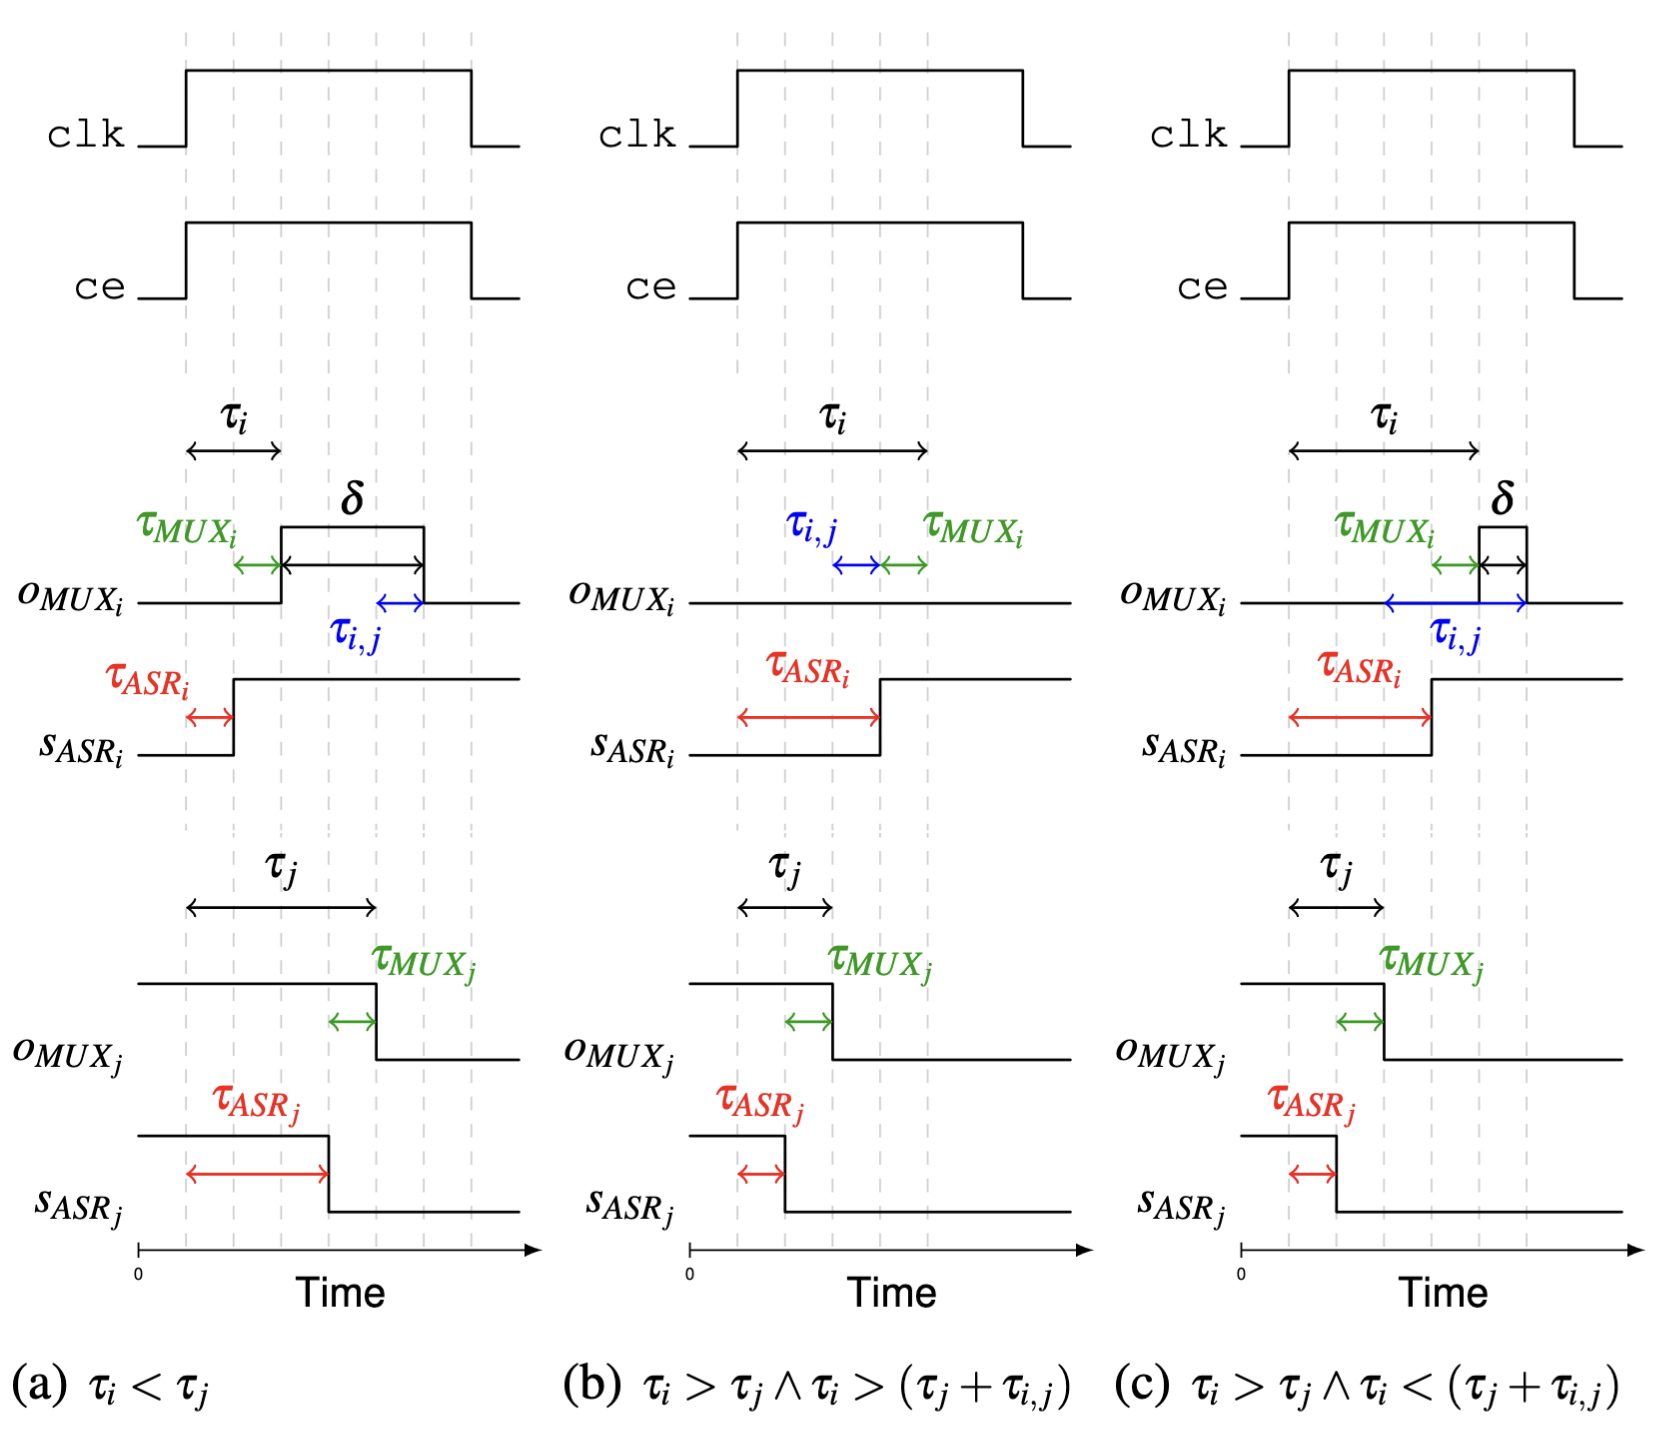
\includegraphics[width=0.8\textwidth]{img/CPUF-Delay-Model.png}
    \caption{CHOICE PUF's three possible delay scenarios. \cite{9556423}}
    \label{fig:CHOICE-PUF-Delay}
\end{figure}

The first case (a) denotes when in the measurement phase the switching of the output signal $s_{ASR_i}$ occurs faster than the switching of the output signal $s_{ASR_j}$, $MUX_i$ propagates the 1 signal from $o_{MUX_j}$ to its output $o_{MUX_i}$ until $MUX_j$ switches to 0, and this is what forms the glitch width $\delta$. Since the delay here is influenced by both the ASR and the multiplexer, we can simplify this case as $\tau_i < \tau_j$, and $\tau_{i,j}$ will contribute greatly to the width of the glitch $\delta$.

When $\tau_i > \tau_j$, $\tau_{i,j}$ becomes decisive in determining whether a glitch will appear at all. As is seen in case (b) where the value of $\tau_{i,j}$ is so small that the output of $o_{MUX_j}$ is always triggered earlier than that of $MUX_i$ and no glitch occurs since $o_{MUX_i}$ stays as 0, this happens if $\tau_{i} > (\tau_j + \tau_{i,j})$.

In the third case (c), $\tau_i$ is still larger than $\tau_j$, similarly to case (b), but this time $\tau_i < (\tau_j + \tau_{i,j})$, i.e. the delay $\tau_{i,j}$ is large enough that $o_{MUX_i}$'s switch to 1 (triggered by $s_{ASR_i}$ after $\tau_i$) still falls inside the window during which the 1 signal coming from $o_{MUX_j}$ is present at the 1-input of $MUX_i$. The observed glitch width is however narrower in this case.

As seen in figure \ref{fig:CHOICE-PUF-Delay}, the created glitch width $\delta$ depends on the absolute differences between $\tau_j+\tau_{i,j}$ and the delay $\tau_i$. It follows that we can estimate $\delta = (\tau_j+\tau_{i,j}) - \tau_i$, and as such we get the equation for the PUF output as:

\begin{equation}
PUF =
\begin{cases}
1 & (\tau_j+\tau_{i,j}) - \tau_i \ge \delta_{min} \\
0 & (\tau_j+\tau_{i,j}) - \tau_i < \delta_{min} 
\end{cases}
\label{eq:puf-out}
\end{equation}

From this we can see that the wider the glitch $\delta$ the higher the probability that we get a 1 as output for the PUF cell, and since this glitch width is dependent on the chosen addresses $a_i$ and $a_j$, then it is possible to find which challenges have the ideal uniformity of 50\%, and this is why the CHOICE PUF is said to be tunable.  


\subsection{Evaluation}
The CHOICE PUF was evaluated on $N=6$ Xilinx Zynq xc7z010clg400-1 boards (labeled $B_0,\dots,B_5$). A 128-bit CHOICE PUF ($Z=128$) was instantiated on each board since 128 bits is a typical length for keys such as an AES key. For every one of the $6144$ possible configurations or challenges $c$ and every board $b$, the PUF was queried $M=1000$ times, yielding responses $r^m_{b,c} \in \{0,1\}^Z$ for $m \in [0,M-1]$. The most frequently occurring response over these $M$ measurements is taken as the nominal response $r^*_{b,c}$, which serves as the reference against which uniformity, uniqueness and reliability are measured.
\begin{figure}
    \centering
    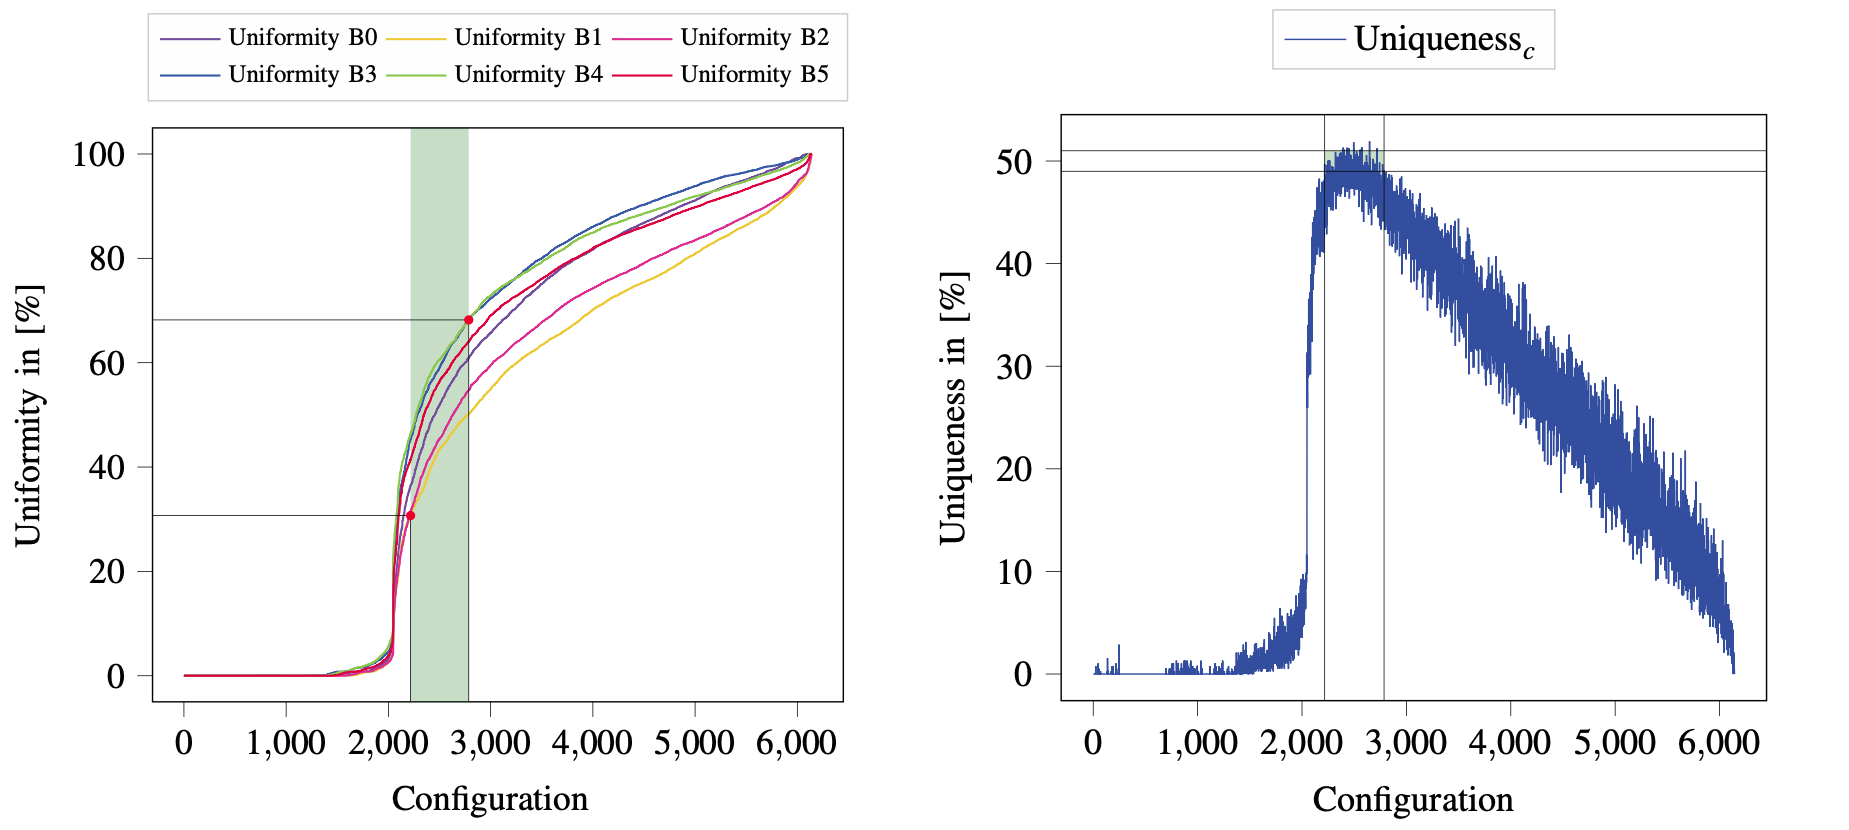
\includegraphics[width=1\linewidth]{img/CPUF-Paper-Unif-Uniq.png}
    \caption{CHOICE PUF uniformity and uniqueness \cite{9556423}}
    \label{fig:CPUF-Paper-Unif-Uniq}
\end{figure}
\subsubsection{Uniformity}
Uniformity measures the proportion of ones in the nominal response:
\begin{equation}
Uniformity_{b,c} = \frac{1}{Z}\sum_{i=0}^{Z-1} r^*_{b,c}(i) \cdot 100\%
\end{equation}
where $r^*_{b,c}(i)$ is the $i$-th bit of the nominal response of board $b$ under configuration $c$. A uniformity close to 50\% is an ideal balance of 0s and 1s in the response, which is desirable for randomness. The left plot on figure \ref{fig:CPUF-Paper-Unif-Uniq} shows the sorted uniformity of all $6144$ configurations for each of the six boards. The curves span the whole range from 0\% to 100\% on every board, which confirms the tunability of the PUF by choosing the appropriate configuration to reach any target uniformity. 

\subsubsection{Uniqueness}
Uniqueness is measured as the average pairwise inter-chip Hamming distance of the nominal responses across all board pairs for a fixed configuration $c$:
\begin{equation}
Uniqueness_c = \frac{2}{N(N-1)}\sum_{i=0}^{N-2}\sum_{j=i+1}^{N-1}\frac{HD(r^*_{i,c},r^*_{j,c})}{Z}\cdot100\%
\end{equation}
A uniqueness close to 50\% is desirable since it means that on average half of the response bits differ between any two boards for the same configuration, which is what allows distinct devices to be differentiated by their PUF responses.
The right plot on figure \ref{fig:CPUF-Paper-Unif-Uniq} shows that uniqueness peaks at around 50\% for the same band of configurations that have uniformity between 30\% and 70\%. Within this band, there are 147 configurations that achieve a uniqueness between 49\% and 51\%, making them the ideal configurations to use in practice.

\subsubsection{Reliability}
Reliability is measured using the Bit Error Rate (BER), which is computed per board and configuration as the average Hamming distance between each of the $M$ measured responses and the nominal response:
\begin{equation}
BER_{b,c} = \frac{1}{M}\sum_{m=0}^{M-1}\frac{HD(r^*_{b,c}, r^m_{b,c})}{Z}\cdot100\%
\end{equation}

An ideal BER of 0\% would mean the PUF's response never changes between measurements, as such, more robust responses tend to have lower entropy. As seen in figure \ref{fig:CHOICE-ber}, on the 147 ideal configuration identified before, the average BER ranges between 2.2\% and 3.8\%, with 13 configurations providing an average BER less than or equal to 2.5\%. To further optimize, each board could select its own best-performing configuration in terms of uniformity and reliability among the 147 to identify itself with.

\begin{figure}
    \centering
    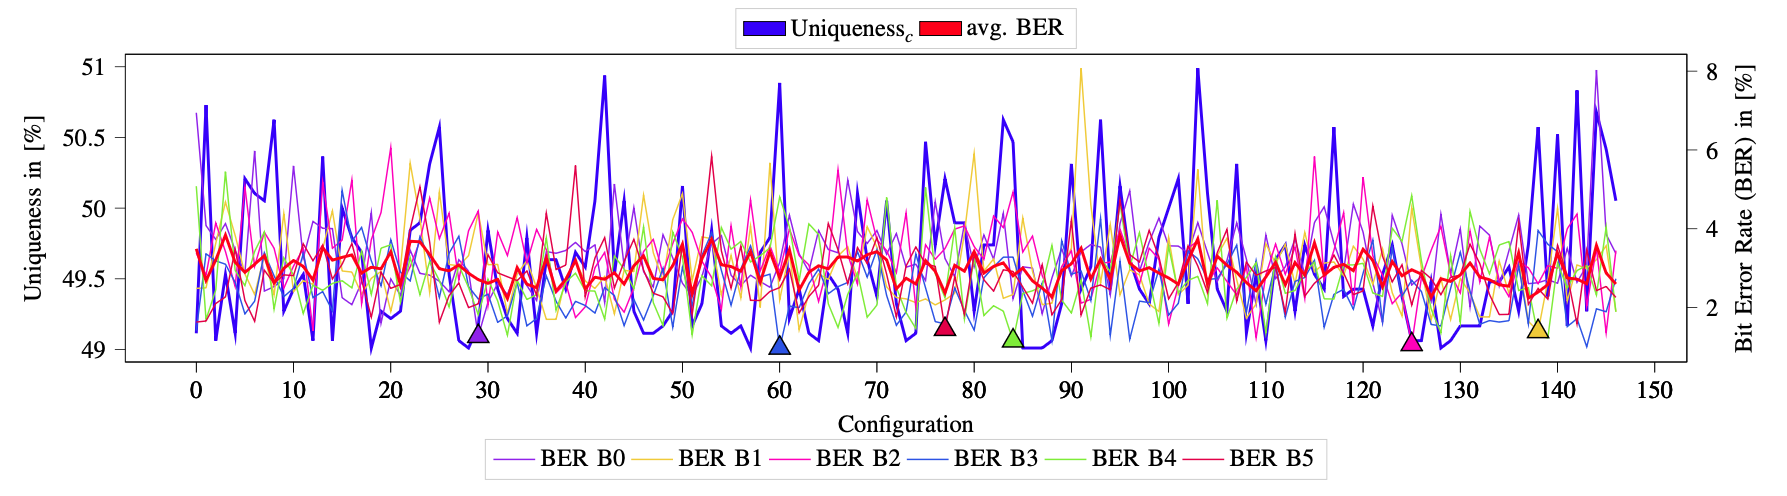
\includegraphics[width=1\linewidth]{img/CPU-BER-Paper.png}
    \caption{Uniqueness and average BER of the 147 ideal configurations \cite{9556423}}
    \label{fig:CHOICE-ber}
\end{figure}

\subsubsection{Footprint}
In the paper, it is mentioned that the CHOICE PUF's footprint is small. However, this is only the case because of the Xilinx SLICEM slice. As we will see in the implementation chapter, the footprint of the CHOICE PUF is quite large when using other FPGA brands.



\section{Logically Reconfigurable PUF (LR-PUF)}
As has been seen in the previous section about PUFs, PUF architectures typically have a fixed challenge-response behavior, this is desirable for applications like device authentication and secure boot since we want the CRP behavior of the device to permanently be tied to its identity. However, other applications would benefit from being able to change or reconfigure this challenge-response behavior after device deployment to for example update or revoke secrets. \cite{10.1007/978-3-642-23951-9_25} refer to PUFs that support this kind of reconfiguration as reconfigurable PUFs and identify two ways of achieving it: physical reconfiguration, where the physical characteristics of the PUF are altered, and logical reconfiguration, where additional logic wraps a normal PUF to change its apparent CRP behavior without physically altering the underlying PUF.

Most physically reconfigurable PUFs rely on optical mechanisms, or reconfigurable hardware such as FPGAs and are therefore hard to use and integrate practically. As such, \cite{10.1007/978-3-642-23951-9_25} introduce logically reconfigurable PUFs (LR-PUF) to enable reconfiguration without the need for complicated measures. It does so by using any normal PUF and wrapping it with stateful control logic that alters the CRP behavior of the underlying PUF. 


\subsection{Architecture}
As show in figure \ref{fig:LR-PUF-Paper}, the LR-PUF exposes two functions: $\texttt{query}_S(c)$ for querying the PUF, and $\texttt{rcnf}()$ for reconfiguring it.

\begin{figure}
    \centering
    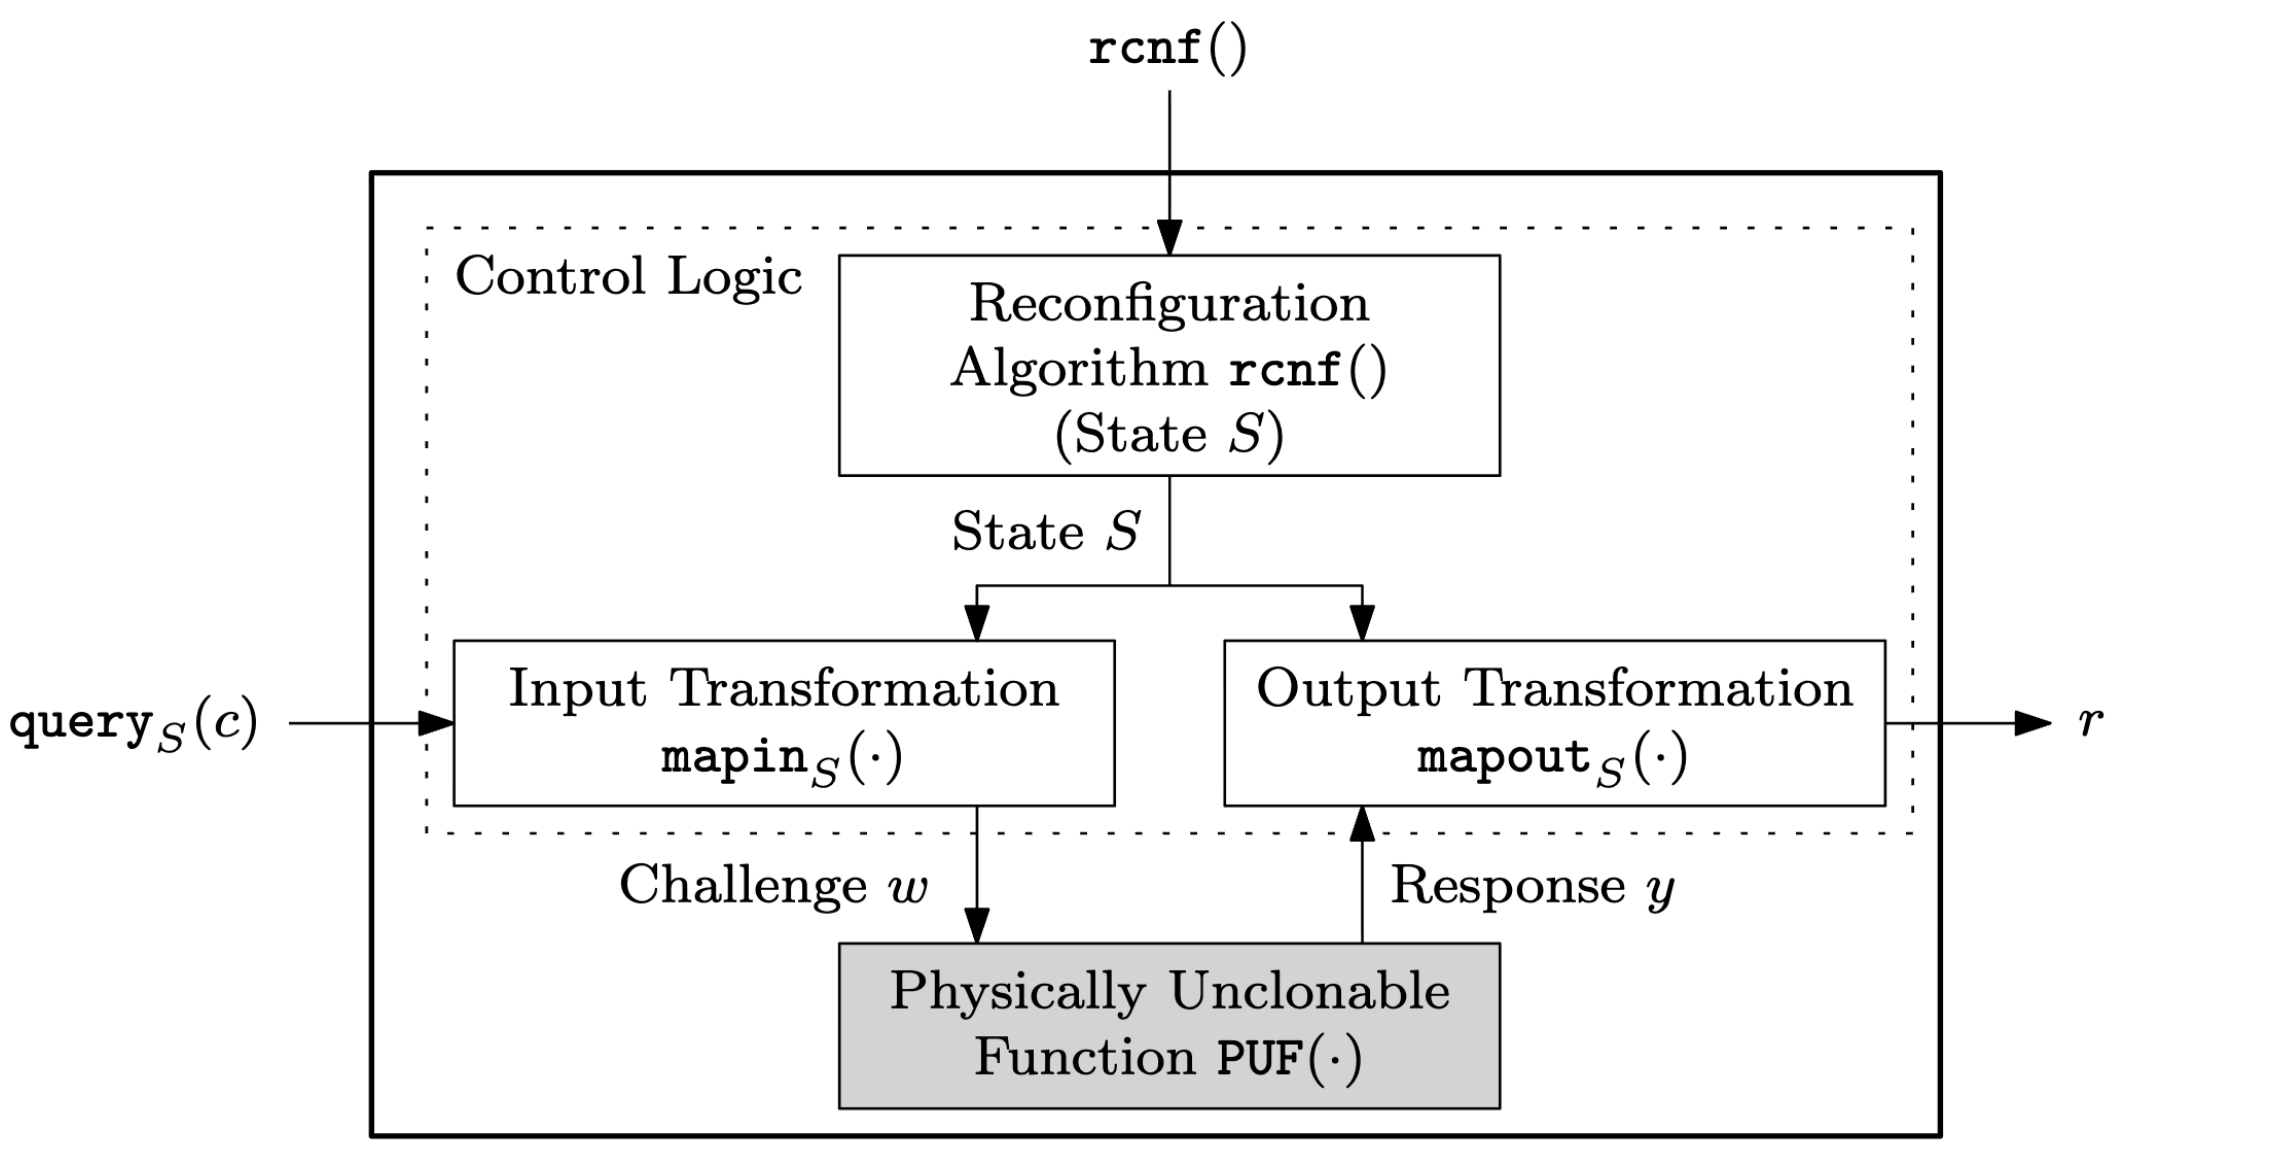
\includegraphics[width=1\linewidth]{img/LR-PUF-Paper-Fig.png}
    \caption{Logically Reconfigurable PUF Architecture \cite{10.1007/978-3-642-23951-9_25}}
    \label{fig:LR-PUF-Paper}
\end{figure}

The function $\texttt{query}_S(c)$ is described in algorithm \ref{alg:LRPUF-query-Paper}. First some challenge $c$ is mapped to another challenge $w$ using the state $S$, then $w$ is used to query the underlying PUF to obtain a response $y$, and finally the response $y$ is mapped out using the state $S$ to get a response $r$. In practice, $\texttt{mapin}_S(c)$ and $\texttt{mapout}_S(y)$ use hash functions to perform the mappings and entangle the state $S$ with the challenge $c$ and response $r$ so that changing $S$ via $\texttt{reconf}()$ (Algorithm \ref{alg:LRPUF-rcnf-Paper}) consequently alters the mapping and along with it the challenge-response behavior.

\begin{algorithm}[ht!]
\caption{$\texttt{query}_S(c)$}
\begin{algorithmic}[1]
    \Require Challenge $c$, current state $S$
    \Ensure Response $r$
    \State $w \leftarrow \texttt{mapin}_S(c)$ 
    \State $y \leftarrow PUF(w)$ 
    \State $r \leftarrow \texttt{mapout}_S(y)$ 
    \State \Return $r$
\end{algorithmic}
\label{alg:LRPUF-query-Paper}
\end{algorithm}

\begin{algorithm}[ht!]
\caption{$\texttt{rcnf}()$}
\begin{algorithmic}[1]
    \Require Current state $S$
    \Ensure New state $S'$
    \State $S' \leftarrow Hash(S)$
    \State $S \leftarrow S'$
\end{algorithmic}
\label{alg:LRPUF-rcnf-Paper}
\end{algorithm}

\newcommand{\Adv}{\mathcal{A}}

\subsection{Threat Model}
The underlying PUF of the LR-PUF is assumed to be physically unclonable and unpredictable. The algorithms for $\texttt{mapin}_S(c)$, $\texttt{mapout}_S(y)$ and $\texttt{reconf}()$ are assumed to be publicly known so as not to rely on security by obscurity. The adversary $\Adv$ is assumed to know the current state $S$ and all previous states of the LR-PUF, but $\Adv$ cannot alter $S$. Based on this threat model, the paper outlined the following properties of an LR-PUF:
\begin{itemize}
    \item \textbf{Backward unpredictability}: $\Adv$ cannot predict the response of the LR-PUF for a previous state to a challenge that has not been queried using that previous state, even if $\Adv$ knows a set of CRPs related to the previous state and can actively query the current state. In other words, once the LR-PUF has been reconfigured, an adversary who only interacts with the reconfigured LR-PUF cannot recover CRPs pertaining to the previous state. 
    \item \textbf{Forward unpredictability}: $\Adv$ cannot predict the response for the current state to a challenge that has not been queried using the current state, even if $\Adv$ knows a set of CRPs related to the previous state and can actively query the current state. In other words, an adversary who has fully compromised the LR-PUF before reconfiguration gains no advantage in predicting its behavior after reconfiguration.
    \item \textbf{Non-resettability}: $\Adv$ cannot set the state of the LR-PUF to a specific value, since this would allow $\Adv$ to trivially break backward unpredictability by resetting the state to a know compromised previous state.
\end{itemize}

The paper argues that non-resettability can be achieved in practice since arbitrarily modifying the state $S$ stored in non-volatile memory through an attack would be uneconomical given the needed precision and equipment.

\subsection{LR-PUF Construction Types}
The paper proposed two implementations of the LR-PUF. The first is optimized for speed and the second is optimized for space.

\subsubsection{Speed-Optimized Construction}
The speed-optimized construction uses a PUF with a large challenge-response space, i.e. a strong PUF. The CRP space must be large for this construction since otherwise it may be possible to enumerate all CRPs. The construction is described in algorithm \ref{alg:LRPUF-speed-query}. When querying, a challenge $w$ is computed by hashing the state $S$ along with the input challenge $c$, then $w$ is used to query the PUF and obtain $y$ which is given as the response $r$ of the LR-PUF. To reconfigure, the state is hashed into itself $S\leftarrow Hash(S)$. Speed here comes from the fact that the hash function is only called once and the PUF is also only queried once. 

\begin{algorithm}[ht!]
\caption{Speed-Optimized $\texttt{query}_S(c)$}
\begin{algorithmic}[1]
    \Require Challenge $c$, current state $S$
    \Ensure Response $r$
    \State $w \leftarrow Hash(S || c)$ \Comment{$\texttt{mapin}_S(c)$}
    \State $y \leftarrow PUF(w)$
    \State $r \leftarrow y$ \Comment{$\texttt{mapout}_S(y)$}
    \State \Return $r$
\end{algorithmic}
\label{alg:LRPUF-speed-query}
\end{algorithm}

\subsubsection{Area-Optimized}
Most PUF architectures with a large challenge space have a small response space, for example the Arbiter PUF. To get more response bits, more PUF cells are needed, but this significantly increases the needed physical area for the PUF. The area-optimized construction queries the PUF $n$ times to allow for more response bits. As described in algorithm \ref{alg:LRPUF-area-query}, a for loop queries the PUF $n$ times by deriving $n$ challenges $w_j \leftarrow Hash(S||c||j)$ and then finally combining their responses $y_j$ into $r \leftarrow (y_0 || \dots || y_n)$.


\begin{algorithm}[ht!]
\caption{Area-Optimized $\texttt{query}_S(c)$}
\begin{algorithmic}[1]
    \Require Challenge $c$, current state $S$, number of sequential PUF evaluations $n$
    \Ensure Response $r$
    \For{$j = 0$ to $n$}
        \State $w_j \leftarrow Hash(S || c || j)$ \Comment{$\texttt{mapin}_S(c)$}
        \State $y_j \leftarrow PUF(w_j)$
    \EndFor
    \State $r \leftarrow (y_0 || \dots || y_n)$ \Comment{$\texttt{mapout}_S(y)$}
    \State \Return $r$
\end{algorithmic}
\label{alg:LRPUF-area-query}
\end{algorithm} 

\subsection{Performance Evaluation}
Both constructions were implemented on a Xilinx Spartan-6 FPGA board. The underlying PUF is an Arbiter PUF with 64-bit challenges and 1-bit responses. Both resulting constructions take 80-bit challenges and generate 64-bit responses. Table \ref{tab:lrpuf-perf-paper} shows their results.

\begin{table}[ht!]
\centering
\caption{Performance results of the speed- and area-optimized LR-PUF constructions \cite{10.1007/978-3-642-23951-9_25}.}
\begin{tabular}{lccc}
\hline
\textbf{Construction} & \textbf{Response time} & \multicolumn{2}{c}{\textbf{Area consumption in slices}} \\
 & \textbf{(clock cycles)} & \textbf{Control logic} & \textbf{Arbiter PUF} \\
\hline
Speed-optimized & 1,069    & 166 & 4,288 \\
Area-optimized  & 64,165   & 358 & 67    \\
\hline
\end{tabular}
\label{tab:lrpuf-perf-paper}
\end{table}

The area-optimized construction requires only about 27\% of the total area required for the speed-optimized construction, but it is about 60 times slower for producing a response. Note that the implementation did not account for the non-volatile memory required to store the state $S$.

\section{Field Programmable Gate Array (FPGA)}
A Field Programmable Gate Array (FPGA) is an integrated circuit whose internal digital logic is not fixed at manufacturing time but can instead be reconfigured to implement almost any digital circuit. It stands in direct contrast to Application-Specific Integrated Circuits (ASIC), whose logic is permanently set during fabrication, and to micro-controller units (MCU), whose fixed hardware can execute sequential instructions. FPGAs stand in the middle between ASIC and MCU. 

\subsection{Architecture}
According to \cite{2018arXiv180503648K}, an FPGA is built from a few recurring building blocks (Figure \ref{fig:fpga-architecture}):
\begin{itemize}
    \item \textbf{Slices}: A slice is a small cluster of look-up tables (LUT) and flip-flops (FF) repeated thousands of times across the FPGA chip. A LUT can be programmed to compute any boolean function of its inputs by writing the function's truth table into it, and an FF is used to store the LUT's output on the next clock edge to build sequential logic. 
    \item \textbf{Programmable Interconnect}: Slices are connected to one another through routing channels and switch-boxes, which are configurable switches that wire one signal path to another.
    \item \textbf{Hardened Blocks}: Some operations are needed so often that building them out of slices would be wasteful. FPGAs therefore embed purpose-specific non-reconfigurable blocks for such operations. The most common are Block RAM (BRAM) for on-chip storage, dedicated micro-processors for running custom firmware, and dedicated DSP (Digital Signal Processing) blocks for optimizing mathematical operations.
\end{itemize}

\begin{figure}
    \centering
    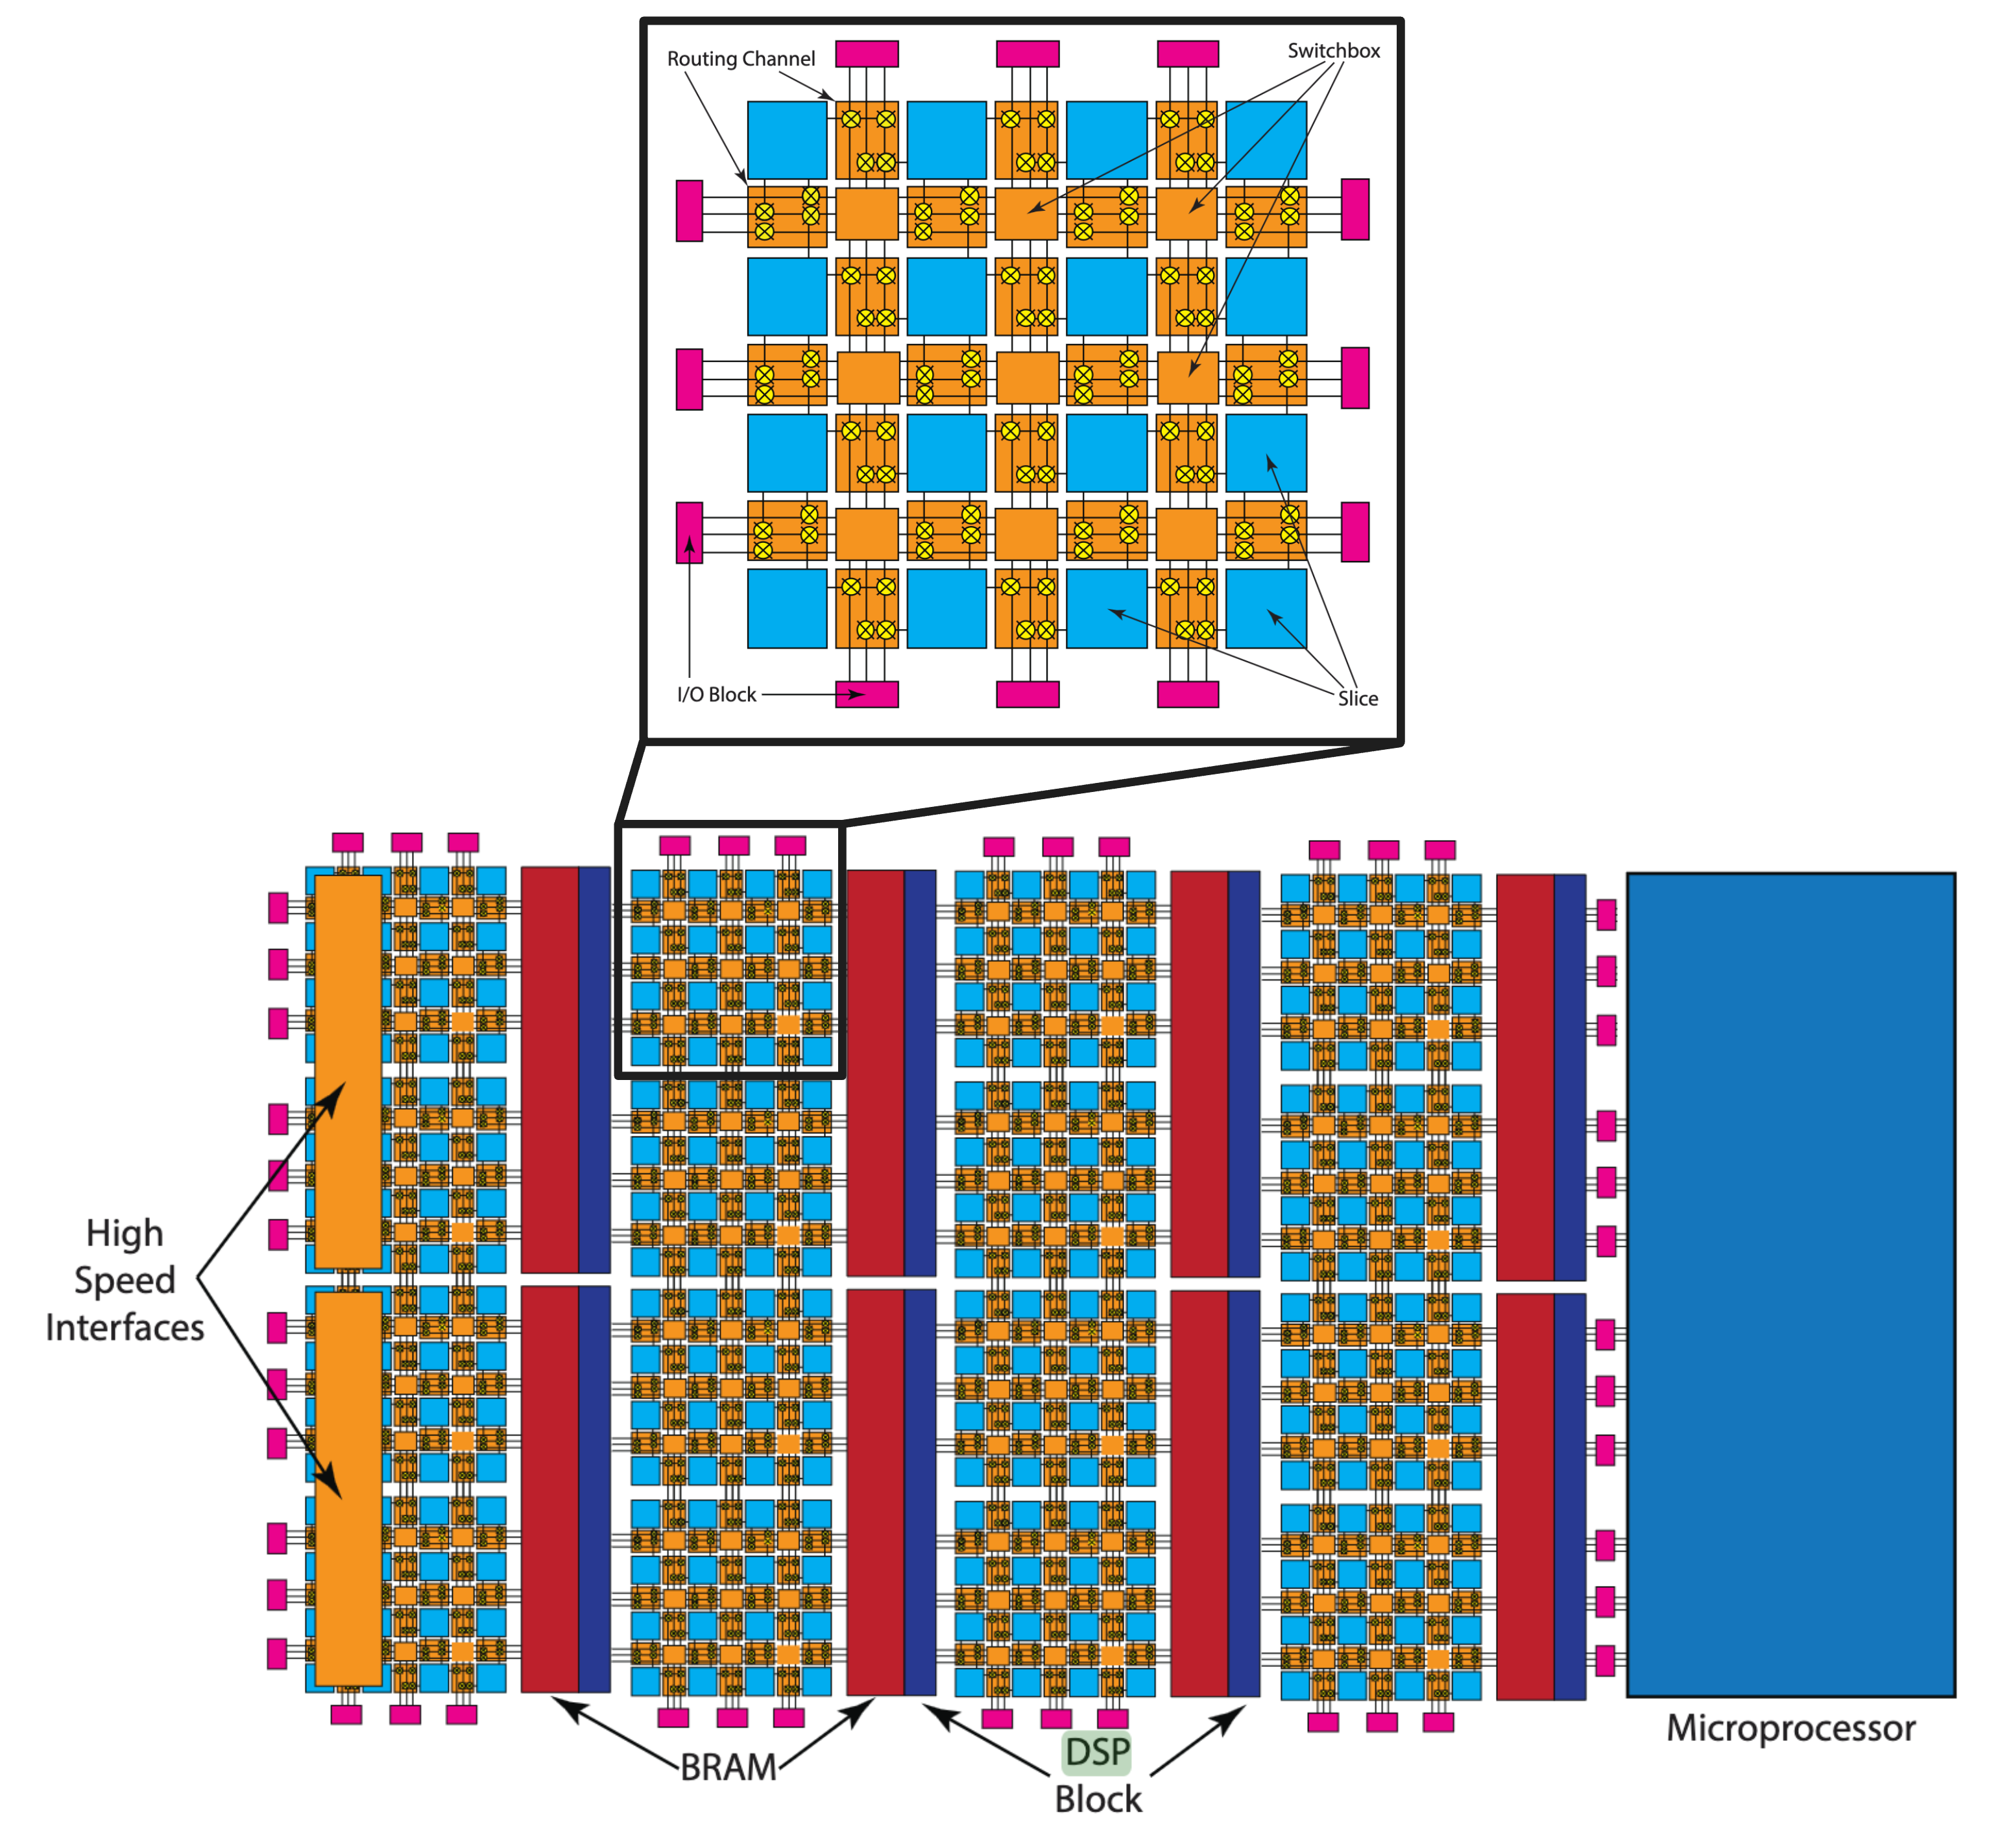
\includegraphics[width=1\linewidth]{img/FPGA-Diagram.png}
    \caption{FPGA Architecture \cite{2018arXiv180503648K}}
    \label{fig:fpga-architecture}
\end{figure}

\subsection{Design Pipeline}
To program a circuit into an FPGA, it must be described using a Hardware Description Language (HDL) such as Verilog or VHDL. The HDL code is elaborated into a Register Transfer Level (RTL) netlist, which is a technology-independent representation that describes the circuit in terms of registers and logic operations. This RTL representation is then synthesized into a netlist of basic logic gates, which are then placed and routed onto the FPGA's actual slices and programmable interconnects, and finally packaged into a bitstream, which is a binary file that configures every LUT, FF and switch on the chip.

\section{Session Hijacking}
Web applications are built on top of the HTTP protocol. HTTP is stateless, which means that by default the server treats every incoming request independently and retains no memory of any previous request from the same client. To identify and authenticate a user across multiple requests, a session is created and used. A session is a period of authenticated interaction that begins once the user successfully logs in and lasts until the user ends it or if it reaches its expiry. Once a session is established, the server issues a session token, which is typically stored in a cookie \cite{rfc6265} to uniquely identify the session. The browser presents this cookie to every subsequent request sent to the server, and the server considers any request carrying a valid token as coming from an authenticated user.

Session Hijacking is an attack in which an adversary obtains a victim's session token and uses it to act as the victim to the server. Because the server authenticates a request purely based on possession of a valid token, a request carrying a stolen token is indistinguishable from a legitimate request. Once the token is in the attacker's possession, they gain full access to the victim's account for as long as the token remains valid without needing to know the victim's credentials. This means that Session Hijacking bypasses Multi-Factor Authentication (MFA), since MFA only protects the initial login step, but once a token is issued, the token alone is sufficient to keep using the session with no further proof of identity required until it expires. This motivates session hijacking countering approaches using Continuous Authentication (CA), where a session is continuously verified during use, so that even a stolen token is not by itself sufficient to keep a session alive.

A session token can be stolen through different means:
\begin{itemize}
    \item \textbf{Malware}: The most common vector is through dedicated cookie-stealing malware, also known as "Infostealer". The victim is tricked into running the malware on their own machine through social engineering \cite{shen2021phishing}.
    \item \textbf{Cross-Site Scripting (XSS)}: If an XSS vulnerability exists in the web app, an attacker can get malicious JavaScript to execute in the victim's browser and exfiltrate the session token stored in the cookies. However, this attack vector is mostly outdated since the new \verb|HttpOnly| flag on cookies makes them inaccessible from JavaScript, but exceptions could exist where some web apps still do not use \verb|HttpOnly| on sensitive cookies. 
    \item \textbf{Network Interception}: An attacker positioned between the victim and the server, for example through an adversary-in-the-middle phishing proxy \cite{evilginx2_kgretzky_2024}, can relay the victim's traffic to the real server and capture the session token as it passes through.
\end{itemize}

\section{PUSH Protocol}
PUSH (PUF against Session Hijacking) \cite{10.1007/978-3-032-07894-0_7} is a protocol that mitigates session hijacking. It works by binding the session to a physical USB dongle whose identity is derived from a PUF, and by periodically requiring that dongle to re-prove its presence for as long as the session remains active. It is the first protocol to apply PUF-based hardware binding to session hijacking for web security. The proposed REPUSH protocol in this thesis builds directly on PUSH.

\subsection{System Model}
PUSH involves four parties (Figure \ref{fig:push-parties}):
\begin{itemize}
    \item \textbf{The dongle}: an external USB device containing an SRAM PUF module and a crypto module. The crypto module is responsible for querying the PUF and deriving cryptographic keys from it to produce digital signatures.
    \item \textbf{PUFMAN (PUF Manager)}: a background service running on the user's device that communicates to the dongle over USB and exposes an API to the browser to allow it to use the dongle.
    \item \textbf{The browser}: acts as the client through which the user communicates with the server or web application.
    \item \textbf{The server}: the web application or service.
\end{itemize}
The dongle, the user's device, PUFMAN and the server are all assumed to be trusted, but the browser is treated as potentially exposed to malicious extensions. PUSH operates at the application layer on top of HTTPS, and assumes that session cookies are handled and stored securely using the standard mechanisms.

\begin{figure}
    \centering
    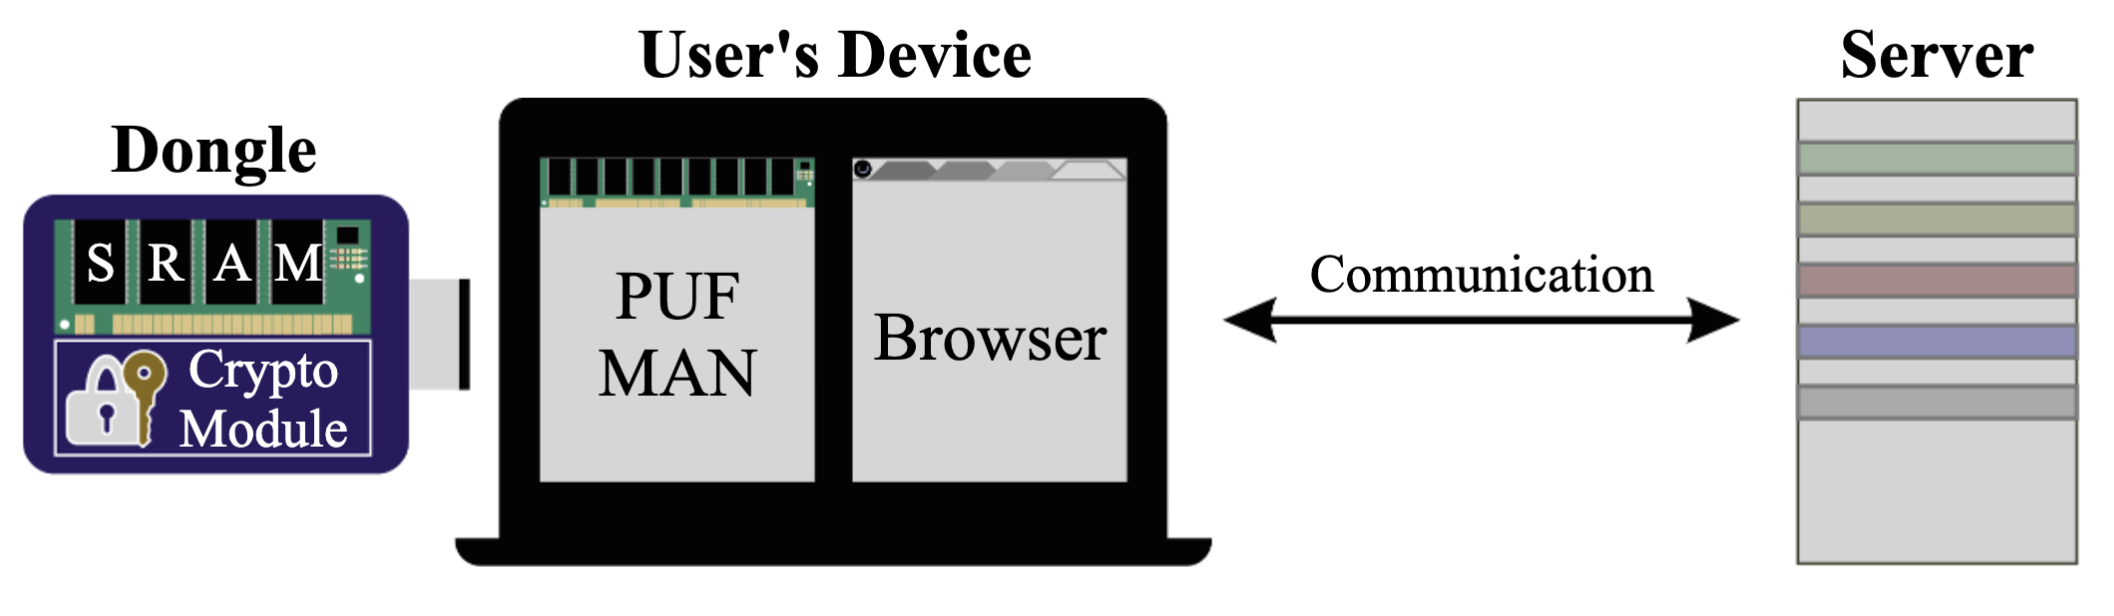
\includegraphics[width=1\linewidth]{img/PUSH-parties.png}
    \caption{PUSH parties. \cite{10.1007/978-3-032-07894-0_7}}
    \label{fig:push-parties}
\end{figure}

\subsection{Protocol Phases}
PUSH is composed of three phases: a one-time dongle initialization, a one-time enrollment with the server, and a recurring operation phase.

\subsubsection{Phase 1: PUF Initialization}
The objective of this phase (Figure \ref{fig:push-init}) is to derive a stable fingerprint from the dongle's SRAM PUF and turn it into a key pair. The crypto module power-cycles the SRAM module $k$ times and reads its contents, which are in this case the SRAM PUF responses. Then the average hamming distance and hamming weight for each memory cell is computed to determine reliable and uniform cells. This filtered set of addresses forms the PUF challenge $C$, and their corresponding bit values form the response $R$. $CRP = (C,R)$ then acts as the unique fingerprint of the dongle. $R$ is processed using a fuzzy extractor to later error-correct it, and the result is used to seed a key generation function $KeyGen()$ for producing a  key pair $(SK, PK)$. Finally, the crypto module signs both $C$ and $PK$ using a secret manufacturer-issued key $SK_D$, and sends $C$, $PK$, and the two signatures to PUFMAN. Once this phase completes, the SRAM module is powered off and both $SK$ and $PK$ are discarded. From now on, the key pair is reconstructed on-demand directly from the PUF rather than being stored on memory.
\begin{figure}
    \centering
    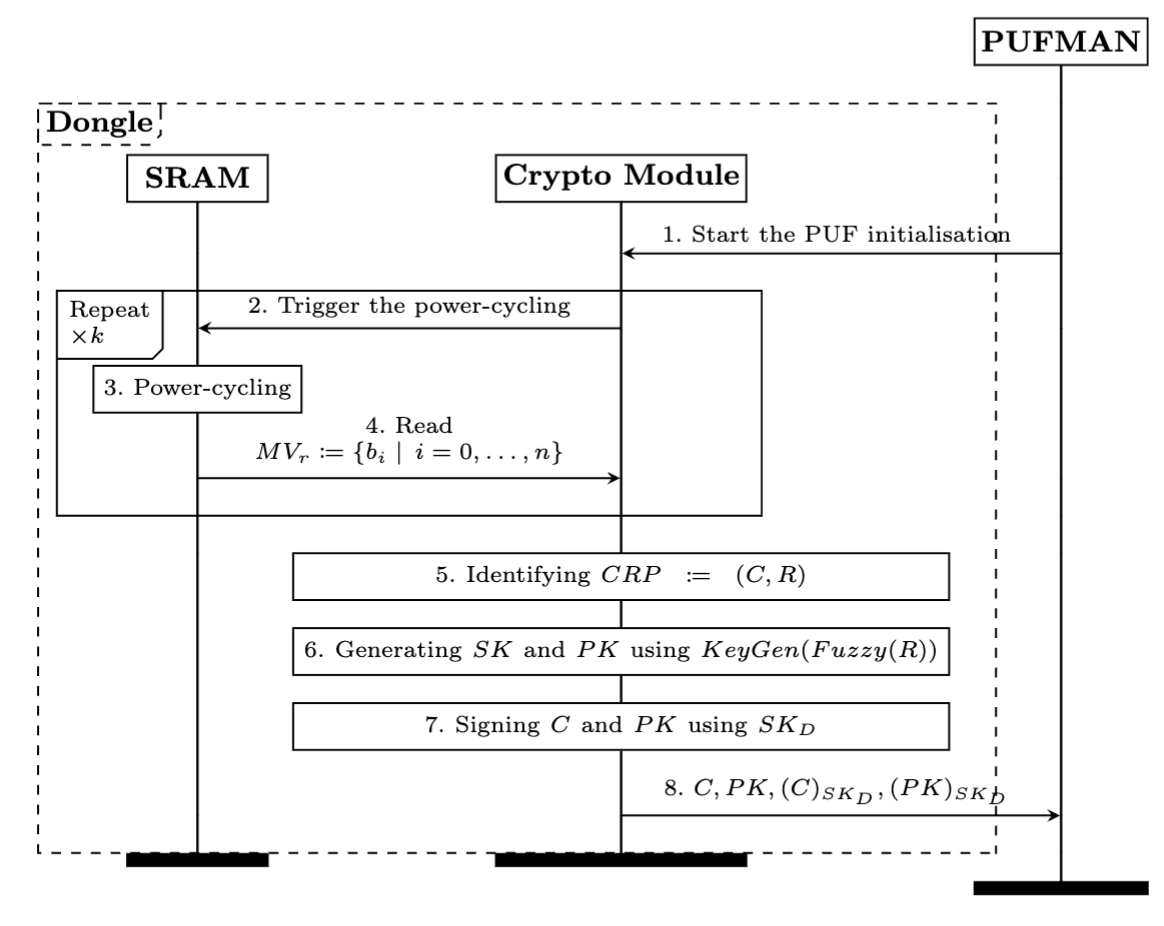
\includegraphics[width=0.7\linewidth]{img/PUSH-init.png}
    \caption{PUSH initialization phase \cite{10.1007/978-3-032-07894-0_7}}
    \label{fig:push-init}
\end{figure}

\subsection{Phase 2: Enrollment}
The user provides the browser with the dongle's manufacturer-issued public key $PK_D$, which the browser uses to validate the produced signatures on $C$ and $PK$ obtained via PUFMAN. The browser does this to confirm that the dongle is genuine. Once validated, the browser sends $C$ and $PK$ to the server as an enrollment request. The server creates a new session for the user, assigns it a session ID, and returns it to the browser as a cookie. From now on, the session is established.
\begin{figure}
    \centering
    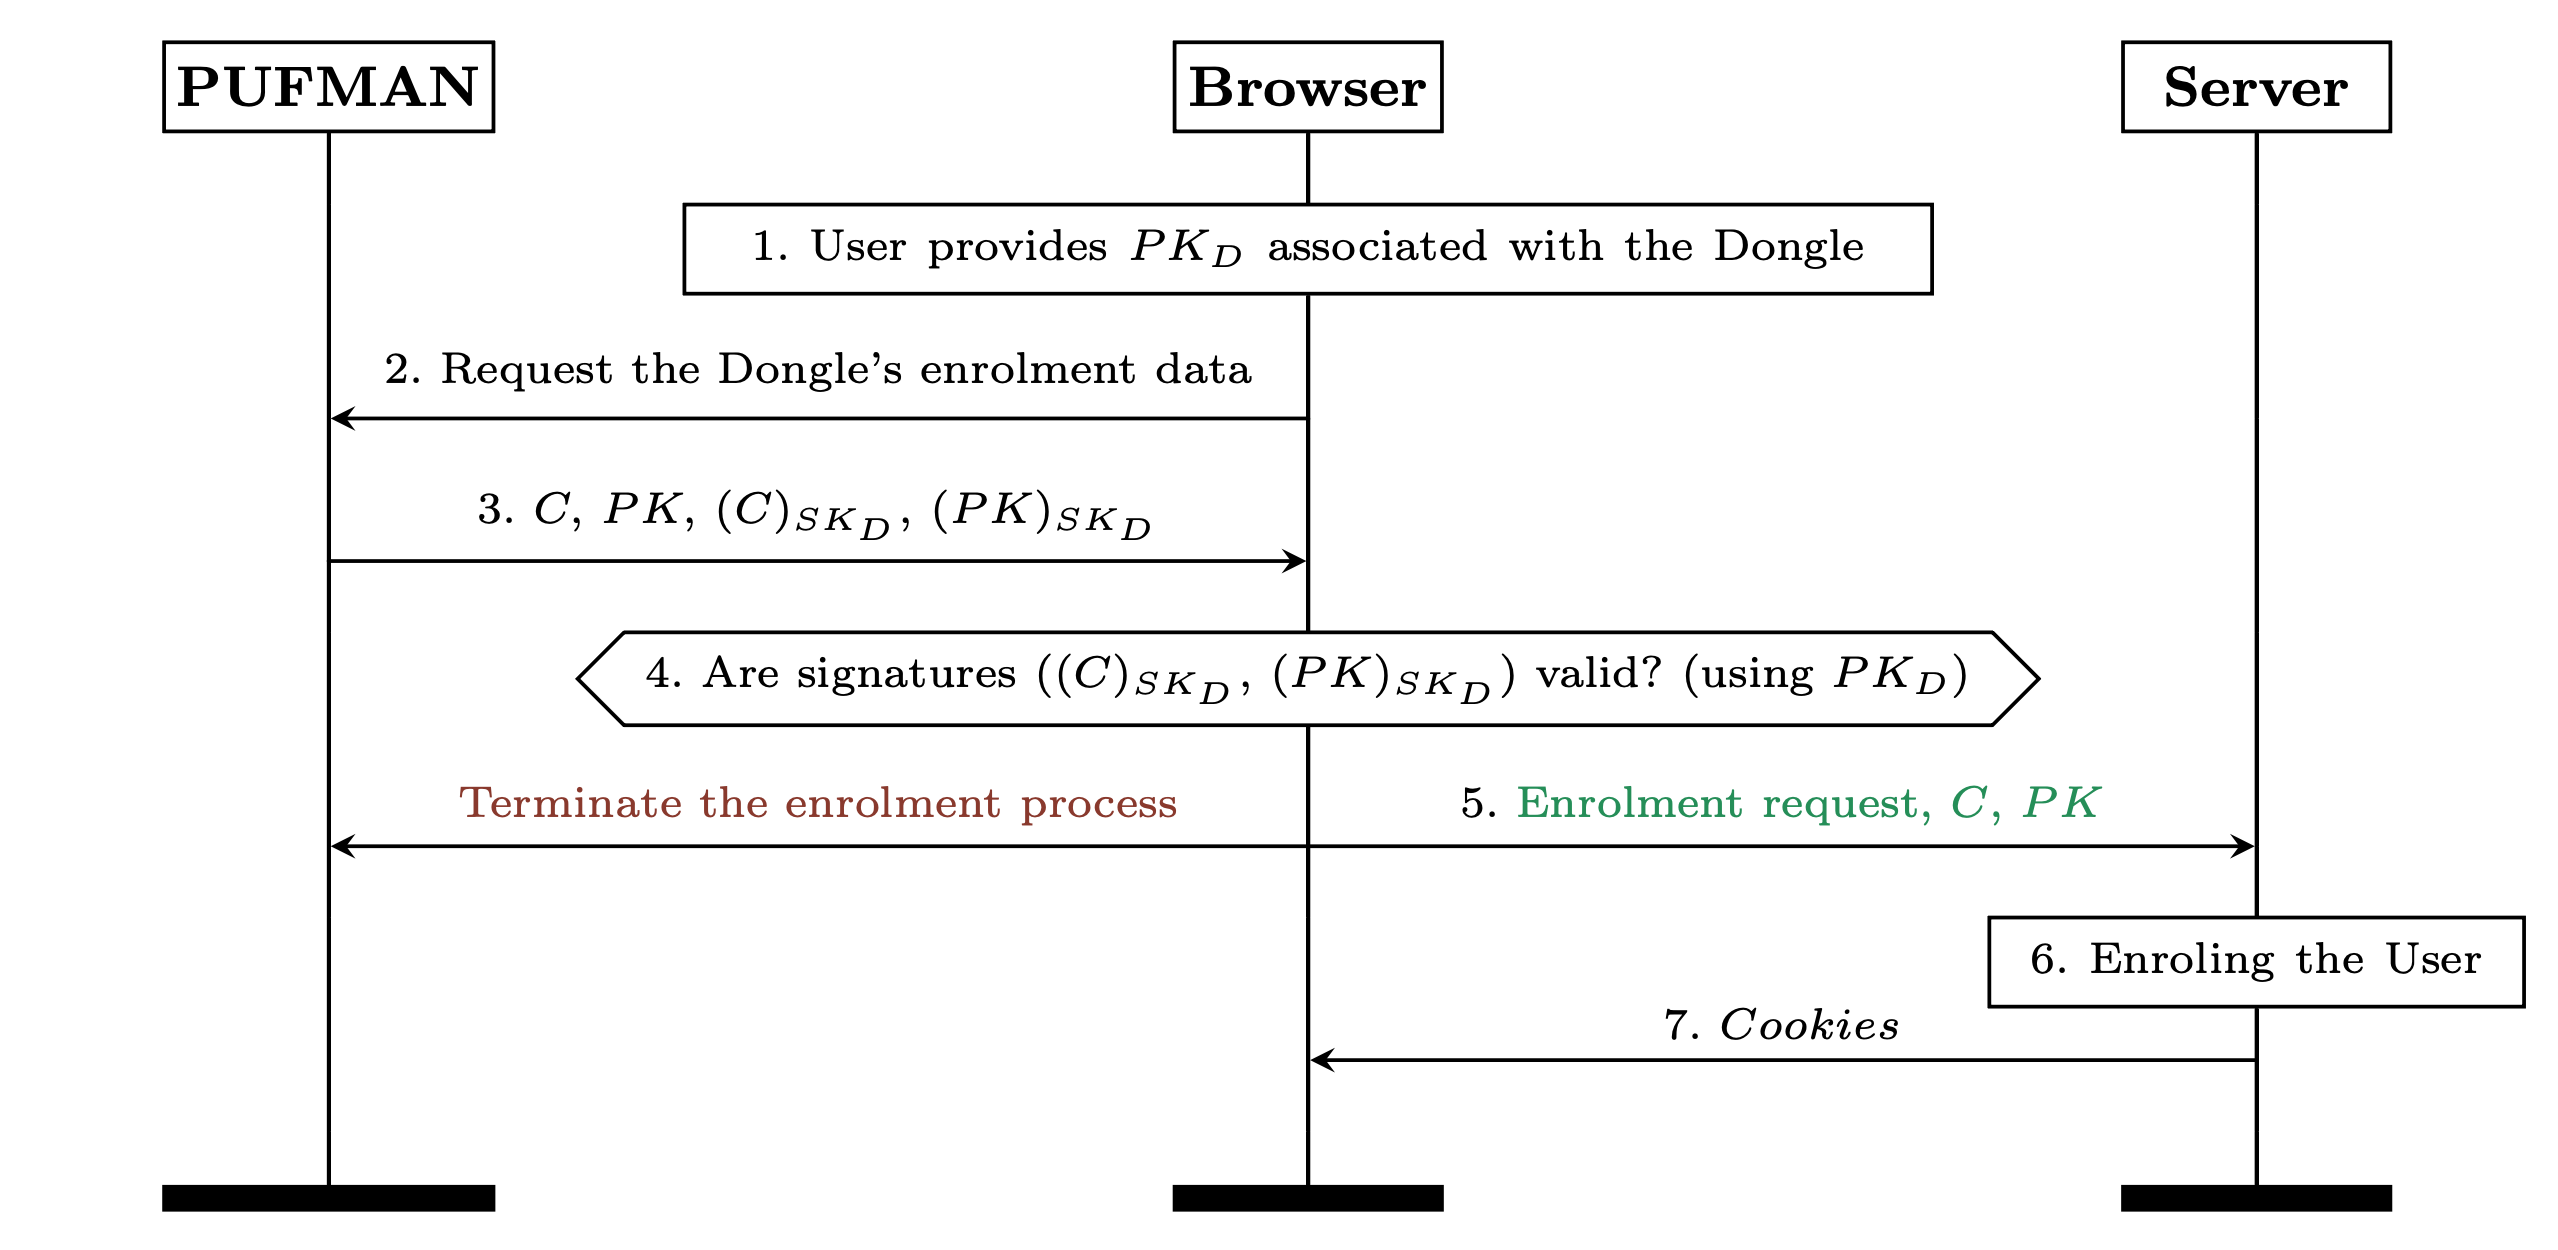
\includegraphics[width=0.7\linewidth]{img/PUSH-enroll.png}
    \caption{PUSH enrollment phase \cite{10.1007/978-3-032-07894-0_7}}
    \label{fig:push-enroll}
\end{figure}

\subsection{Phase 3: Operation}
For every subsequent request, the browser attaches the cookie to it as usual. However, the server periodically responds by also including the enrolled challenge $C$ together with a freshly generated nonce $N$ to be signed along with the cookie by the dongle. This request is relayed to the dongle via the browser and PUFMAN. The dongle queries the SRAM PUF by powering on the SRAM and reading the response $R$ using the addresses specified by $C$. Since this new reading $R$ is subject to noise, it must be error-corrected using the fuzzy extractor before using it to regenerate the key pair $(SK,PK)$ derived in phase 1. $SK$ is then used to sign $N$ and the cookie. The resulting signatures are relayed back to the server, which will either accept them if the nonce $N$ is fresh and both signatures are correct under $PK$, otherwise, the session is terminated. Requesting a signature on every single request would introduce noticeable latency, so instead the signature is treated as valid for a specific validity window and is refreshed shortly before it expires at some update time $T_{update} < T_{validity}$. A shorter $T_{validity}$ terminates a hijacked session more quickly, but requires more frequent signing.
\begin{figure}
    \centering
    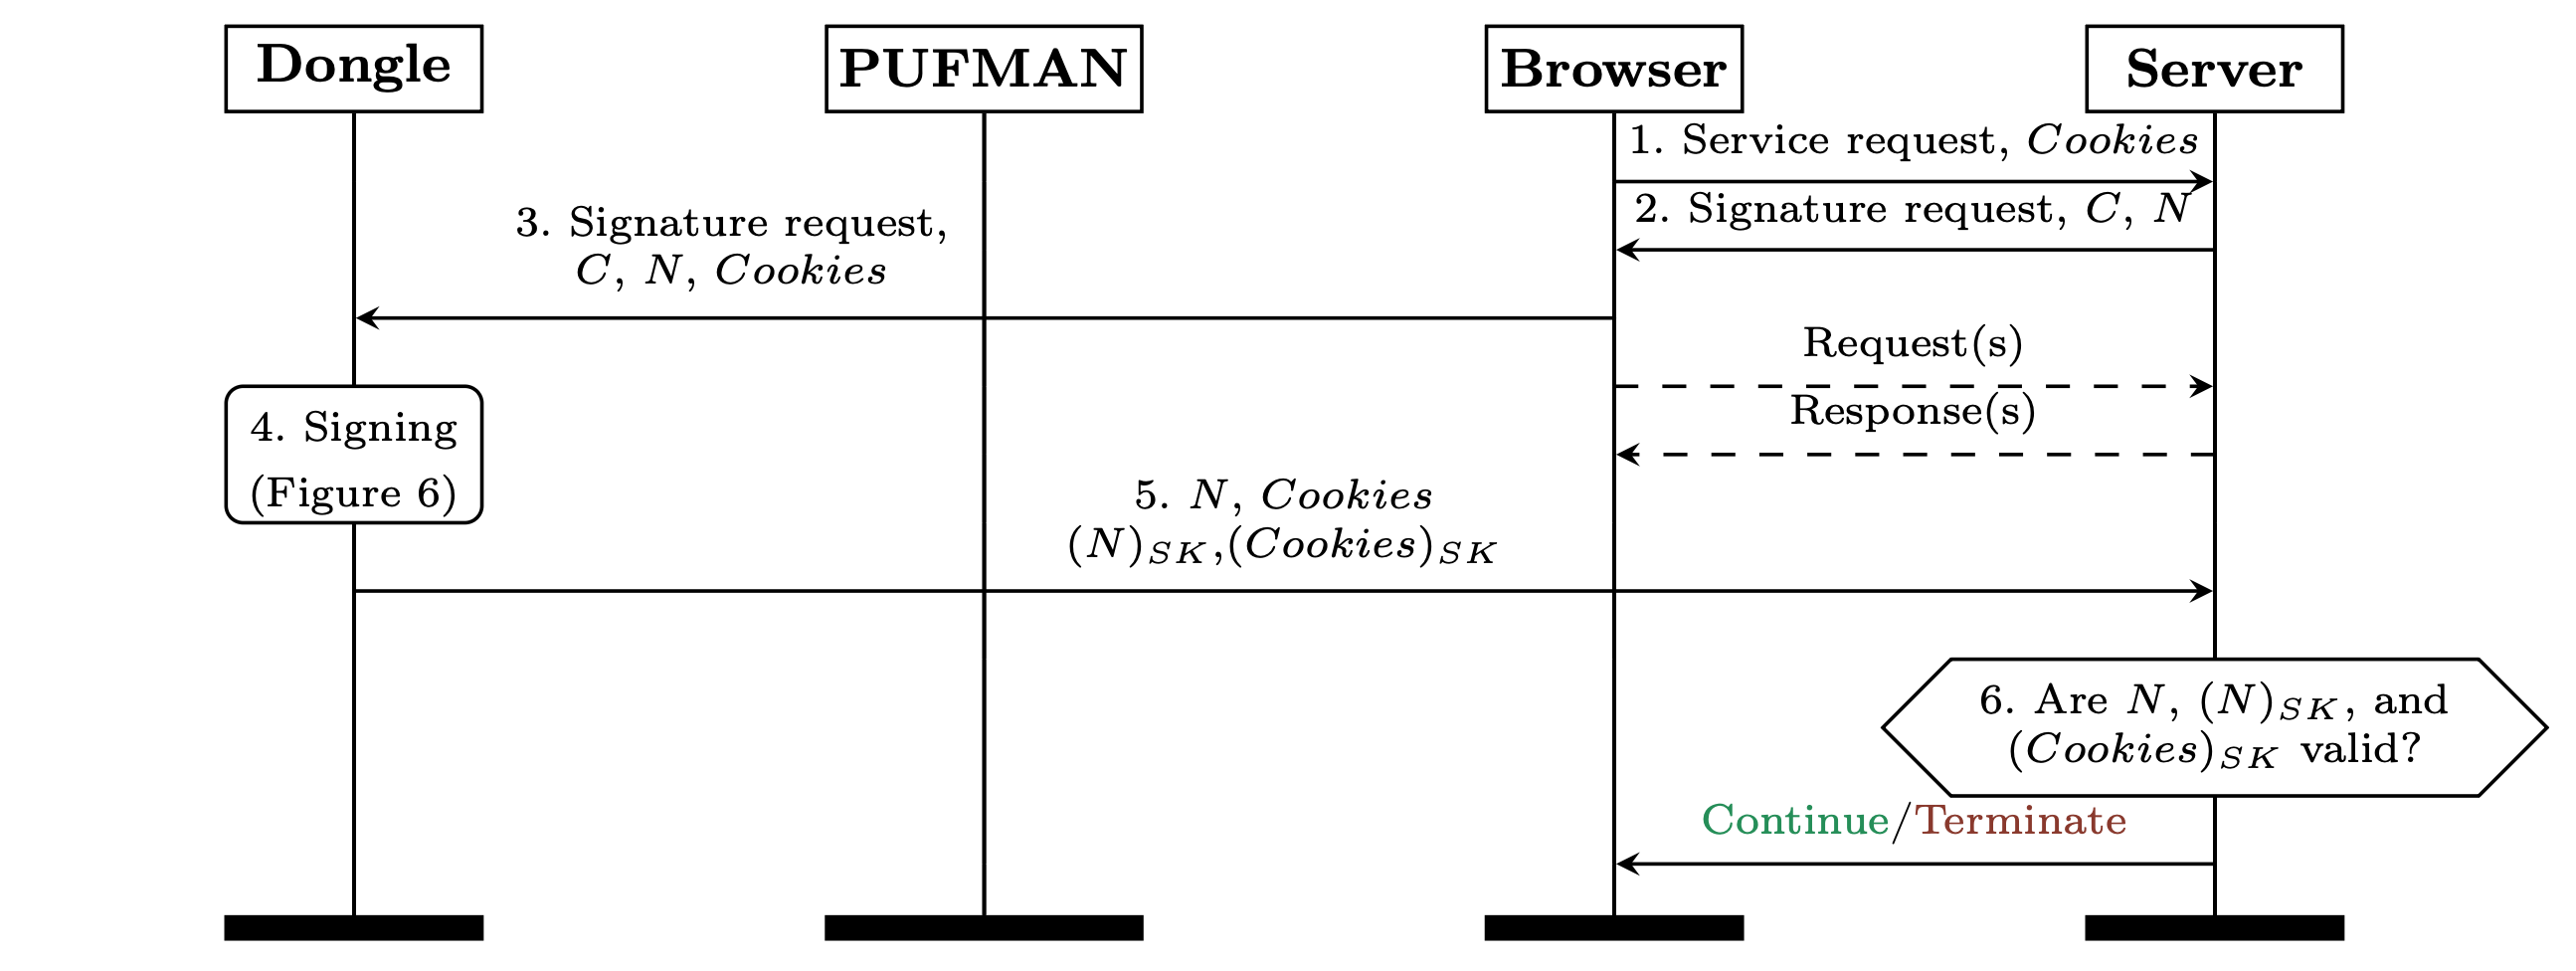
\includegraphics[width=0.9\linewidth]{img/PUSH-oper.png}
    \caption{PUSH operation phase \cite{10.1007/978-3-032-07894-0_7}}
    \label{fig:push-oper}
\end{figure}

\subsection{Performance and Limitations}
In PUSH's proof-of-concept implementation, the dongle is built using an Arduino Nano 33 BLE board with an external SRAM module and Curve25519 signing. Phase 1 for PUF initialization took around 11 seconds, which is dominated by the time need to power-cycle the SRAM three times ($k=3$). Phase 2 for enrollment took around 2 ms. The signing during the operation phase took in average 419 ms. Since initialization only runs once and the signatures only happen periodically, PUSH introduces very little latency in practice.

PUSH has some limitations. For example, PUSH's scalability is bounded by the size of the SRAM PUF. Since each session requires its own unique CRP, the total number of concurrent sessions the dongle can support is limited by how many disjoint CRPs can be extracted from the SRAM. The other limitations were discussed as part of the introduction to this thesis.


% !TeX encoding = UTF-8
% !TeX spellcheck = en_GB
% !TeX root = ../thesis.tex

\chapter{Related Work}
\label{chapter:related_work}
\section{PUFs on FPGAs}
Numerous PUFs suitable for implementation on FPGAs have been proposed. However, very few publications (two to our knowledge) provide the source code of their designs, limiting reproducibility, external evaluation, and practical reuse or extension in future works. As highlighted by \cite{6546024} and \cite{6645555}, one of the main motivations for implementing PUFs on FPGAs is the protection of hardware intellectual property (HW-IPs) by binding it to specific FPGA devices. The hardware IP protection consists of protecting the generated bitstream, which is the final compiled output from the hardware description source code that is used to program the FPGA. This bitstream is typically stored on insecure flash memory on the same board as the FPGA. If the bitstream is illegally copied, this can lead to revenue loss due to it being intellectual property. Such IP is very valuable since it is the main product of companies that build application specific high performance processors (ASHPP) using FPGAs. Previous binding techniques rely on trusted third parties for public-key encryption \cite{4439246} and store keys on secure ROM or flash memory, which exposes the IP to side-channel attacks. Researchers are therefore investigating the usage of PUFs on FPGAs as a safer and cheaper alternative for storing secrets critical to IP binding mechanisms.


\cite{stephan_nolting_2021_5706593} implemented and briefly tested a 96-bit ring oscillator PUF on various FPGA boards, but found that only 63 bits were stable enough for a reliable response. He also observed that repeated successive queries increased the likelihood of bit flips, which he attributes to a rise in chip temperature. While the high number of successive queries (4096 to be exact) can be justified when using response processing methods such as voting or hysteresis - where a bit is considered "stable" if it is consistently set (to 1) or cleared (to 0) above a given threshold, this introduces trade-offs between reliability, query speed, and thermal constraints when using FPGA PUFs in practical devices. The need for such a high number of measurements could be mitigated by using error-correcting codes (ECCs), which would allow occasional unstable bits to be corrected without the need for repeated measurements.
\cite{9556423} designed and implemented a new delay-based PUF called CHOICE PUF. The proposed PUF supports 6144 challenges but can be adapted to support more. One particularity of the CHOICE PUF is that it is tunable, meaning that they could increase or decrease the probability of obtaining 1's in the PUF response using the properties of the challenges. They also found that 147 of the 6144 challenges provided a uniformity rate between 49\% and 51\%. Furthermore, on the 147 challenges with desirable uniformity, the error rate went up to 4\% and as low as 1.5\%, making it a very reliable PUF. The same 147 challenges also had inter-PUF uniqueness near 50\%.
In an effort to reduce the footprint of PUFs on FPGAs for allowing the FPGA to be used for other applications while still housing a PUF, \cite{5547067} propose time division multiplexed PUFs (TDM-PUFs), which is a method to divide one long PUF into several smaller PUFs that run in different times by exploiting the dynamic partial reconfiguration (DPR) feature available in most FPGAs, which allows reconfiguring the FPGA during operation to use the same hardware resources for different purposes in different time segments.

As summarized by \cite{cryptography7040055}, whilst FPGA-based PUF designs provide advantages for device authentication and key generation, they also introduce important trade-offs. Notably, the reliability of PUF responses can be affected by environmental factors such as temperature. Also, the wide variety of existing FPGA-based PUF designs introduces challenges in terms of standardization and scalability, as the PUF implementations may require significant FPGA resources or careful placement and routing constraints, which can limit scalability when large CRPs are needed.

\section{Reconfigurable PUF}

Reconfigurable Physical Unclonable Functions (R-PUF) are PUFs whose challenge-response behavior can be updated. \cite{10.1145/1502781.1502786} first proposed leveraging FPGA reconfiguration to modify a PUF's behavior. \cite{10.1007/978-3-642-23951-9_25} later formalized the concept with Logically Reconfigurable PUFs (LR-PUFs), which use an internal state to remap challenges and responses without modifying the underlying hardware. Invoking a reconfiguration function replaces the old state with a new one (e.g: through hashing), producing a new CRP set. For a more practical implementation of an LR-PUF, \cite{LR-PUF-Memory-Based} introduce a memory-based LR-PUF that combines an SRAM PUF with a non-volatile state in NVM (non-volatile memory), the response of the PUF is concatenated with the current state and hashed to hide the PUF's behavior and protect it from potential modeling attacks. The key principle is that the new behavior of the PUF after reconfiguration is unpredictable from the previous one. This hiding of the PUF's behavior protects it against cloning or modeling attacks. 

\cite{10.1145/3274666} classified R-PUFs into two categories. The first is circuit-based R-PUFs, where the physical circuit is reconfigured (e.g: via FPGA routing) to produce a new hardware instance of the PUF. For example, \cite{DPUF} propose a reconfigurable DRAM PUF based on refresh pausing, where the reconfiguration is done by changing the refresh-pause interval to alter the CRPs generated by the PUF. The second category is algorithm-based R-PUFs, where the hardware remains the same but the challenge-to-response mapping is altered through extra logic. As proposed by \cite{10.1007/978-3-642-23951-9_25}, a transformation is applied to an input challenge using the current state, and similarly another transformation is applied to the output using the state. Here, the configuration of the PUF is simply comprised of extra steps that are applied on its output and inputs.

Reconfigurable PUFs are leveraged in security protocols where they are used in IoT scenarios to provide fresh keys and counter replay or modeling attacks. For example, \cite{10549865} propose a mutual authentication protocol where an R-PUF is reconfigured after each session to limit the exposure of its CRPs. \cite{s22155577} propose an R-PUF-based authentication framework for FPGA-based IoT devices, where the previously mentioned dynamic partial reconfiguration feature is used to reconfigure the PUF by changing its placement at runtime.

Because reconfiguration scrambles the CRP mapping each time, R-PUFs offer strong security advantages. \cite{10.1007/978-3-642-23951-9_25} proves forward- and backward-unpredictability of their LR-PUF model, i.e. responses measured before the reconfiguration are invalid after it, and an attacker with access to a reconfigured PUF cannot estimate the PUF behavior before reconfiguration.


\section{Methods Against Session Hijacking}
The most commonly used method for preventing session hijacking in web communications is the HttpOnly cookie attribute introduced in RFC6265 \cite{rfc6265}. The HttpOnly attribute prevents JavaScript from directly accessing session cookies, thereby preventing attacks in which cross-site scripting (XSS) is used to steal cookies. Another used attribute is the SameSite cookie attribute \cite{ietf_rfc6265bis_draft} which restricts where browsers send cookies to mitigate previous cases where sensitive cookies were unintentionally transmitted to malicious sites upon visit. While these mechanisms cover some attack vectors leading to session hijacking, the session cookies may still be compromised through other means such as malware \cite{tyler2025browsercontrolsprotectcookies, cookieMiner_unit42_2019} or network interception \cite{evilginx2_kgretzky_2024} as described in \cite{mitre_t1539}. As a result, several research efforts have explored methods to tackle session hijacking at a deeper level.

With the exception of the aforementioned PUSH protocol, no approach to defend against session hijacking in web communications uses PUFs, rather the usage of PUFs is mostly limited to IoT authentication schemes where they are used as a source of random numbers \cite{10.1007/978-3-540-88625-9_3}, unique identifiers \cite{9557280} or cryptographic keys \cite{10538739, 10007641}. 

The methods for protecting web communication or any other kind of communication against session hijacking usually involve binding a session to some other variable through continuous authentication (CA), where the user is repeatedly authenticated throughout the session using contextual signals rather than relying solely on the initial login; for instance, the variable could be user behavior \cite{6879297, 8757539}, user location \cite{5692487}, device characteristics \cite{9530399}, or biometrics \cite{https://doi.org/10.1002/widm.1365, 8010662, 6424854}. \cite{8757539} propose an adaptive CA method that models the keystroke patterns and mouse usage behavior patterns of a user to continuously verify identity during a session. \cite{9530399} propose an IoT CA protocol that involves devices features such as the battery level and device location. \cite{6424854} evaluate the usage of biometrics in CA and adapts the session timeouts based on user activity and biometric data quality. 

Other approaches focus on limiting the exposure of session cookies. For example, \cite{10.1007/978-3-642-19125-1_7} tackle the problem preemptively by limiting the exposure of the session cookies to XSS attacks through hiding the session cookies from the browser through an external proxy. Similarly, \cite{10.1007/978-3-319-64701-2_7} developed a proxy to detect and drop any illegitimate transfer of cookies. Device Bound Session Credentials (DBSC) \cite{w3c-dbsc} propose binding sessions to device-protected cryptographic keys, typically secured using hardware such as a Trusted Platform Module (TPM), instead of only relying on bearer cookies. 

A separate class of session protection mechanisms relies on one-time session tokens. Such protocols prevent replay attacks by generating a fresh token for each request. \cite{He2020} propose and evaluate a one-time cookies (OTC) protocol based on a novel hash-based one-time password (OTP) protocol, which unlike traditional OTP approaches does not rely on time synchronization or on a fixed shared key for an entire session, rather multiple hash chains are established during login to generate one-time values that encrypt and authenticate each subsequent request.

Each of the aforementioned approaches presents its own advantages and limitations. For some methods, the deployment often introduces additional complexity and infrastructure requirements, making them more suited for environments with high security requirements. Others are easier to integrate, but offer weaker protection. Some use AI or heuristics for continuous verification, which introduces false acceptance rates (FAR) and false rejection rates (FRR), whereas others are grounded on solid mathematically proven cryptographic protocols. As a result, defending against session hijacking is a trade-off between security, usability, and ease of deployment. This compromise is important to keep in mind when considering methods against session hijacking.

% !TeX encoding = UTF-8
% !TeX spellcheck = en_GB
% !TeX root = ../thesis.tex

\chapter{Architecture/System Design}
\label{chapter:design}

The REPUSH (Reconfigurable PUF against Session Hijacking) protocol is designed to address a fundamental flaw in current session security: the absence of trusted continuous authentication after the initial login event. Existing continuous session validation approaches totally trust the host machine to faithfully mediate all interactions between the user and the server. In practice, the main attack vector for session hijacking is cookie theft. Such theft is carried out through specialized malware, so called "Infostealers", which the victim runs on their machine through some elaborate social engineering trick. 

The main observation motivating REPUSH is as follows: if the "Infostealer" malware has remote code execution abilities, which is a prerequisite for cookie theft, then it follows that this same malware could be adapted to further exploit any kind of continuous session validation scheme that the user is using. To give an example with the previously presented PUSH protocol, any malware could in theory use the dongle to sign cookies and silently prove ownership of the dongle. The host computer's role as a trusted intermediary is what makes this attack possible. 

REPUSH eliminates this attack surface by assuming that the host is potentially compromised. Similar to PUSH, REPUSH uses an external dongle as proof of ownership of a session. Under this new threat model, the dongle must be adapted so that the compromised host does not exploit it. Another key improvement is the use of an LR-PUF to augment a weak PUF for fast ephemeral key generation. In this chapter, we will explore the design goals and security requirements that motivate the REPUSH protocol, define the threat model and assumptions under which the protocol operates, introduce the protocol parties and their respective roles, define each phase of the protocol in detail, and describe the logical design of the dongle. In doing so, this chapter addresses research question 1 by redesigning the PUSH protocol around a fully compromised host threat model, and it addresses research question 2 by explaining how the LR-PUF's reconfiguration property is integrated into the protocol.  

\section{Design Goals and Security Requirements}
Balancing between security and usability is a delicate act that requires careful design. REPUSH is driven by two goals: security goals which define the threats that the protocol must protect against, and usability goals which ensure user-friendliness and that the protocol remains practical for deployment. 

\subsection{Security Goals}

The protocol's primary security requirement is continuous session authentication: a session token or cookie obtained by the attacker should be insufficient to own the session. Rather, ownership of the dongle must be demonstrated at specified intervals, and sensitive requests must be signed by the dongle after explicit approval by the user on the dongle's user interface. 

Since the host computer is not trusted, all cryptographic operations such as signing and encryption, key storage, and user approval should occur exclusively within the dongle which will act as an isolated trusted computing environment. Furthermore, the protocol is designed according to the least privilege principle, which means that each party only holds the data it needs to carry out its role in the protocol. 

The protocol should also provide mutual authentication, i.e. the dongle must verify the server's identity, and the server must verify that the dongle does belong to some user. 

Since sensitive requests must be approved on the dongle's own user interface, the user has full transparency on the requests they make to the server. A compromised host cannot compromise the dongle, as in even if it were to make a request to it, the dongle will clearly and transparently show what that request is on its screen. This trusted display concept \cite{ledgertrusteddisplay} is similar to how some cryptocurrency physical wallets have a screen which shows which receiving address will receive the cryptocurrency to avoid sending it to another address in case the user's computer is compromised (see figure \ref{fig:trusted-display}). 

As a further consequence of this user intent confirmation on a trusted display, we get passive compromise detection. Because every sensitive request must be approved by the user on the dongle's screen, any attempt by malware to invoke a signing operation for a sensitive request will immediately alert the user, as they would see a request they did not intend. This acts as a way to detect intrusion and then independently take the necessary precautions and steps to remediate it. Unlike traditional intrusion detection systems running on the host, the dongle provides a reliable intrusion indicator of compromise that even the most privileged of malware cannot bypass.

\begin{figure}[ht!]
    \centering
    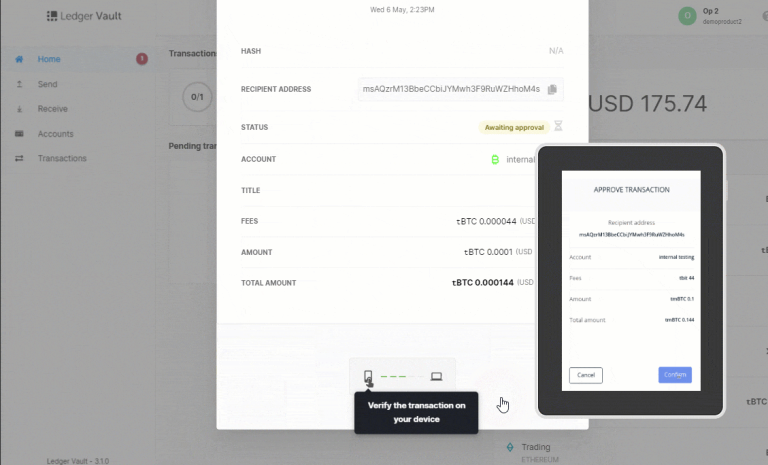
\includegraphics[width=0.8\textwidth]{img/ledger.png}
    \caption{Trusted display on Ledger wallet to confirm a transaction. \cite{ledgertrusteddisplay}}
    \label{fig:trusted-display}
\end{figure} 

\subsection{Usability Goals}
Security mechanisms that produce excessive friction are circumvented or disabled by users. The security goals must therefore be supplemented with usability goals to reduce friction. To this end, the protocol distinguishes between high risk sensitive and low risk non-sensitive requests. Similar to standard requests in PUSH, non-sensitive requests are processed and accepted by the server without any user interaction within a validity window $T_{Validity}$ which will be explained in more detail in the protocol design section. On the other hand, sensitive requests require explicit approval on the dongle's touch screen. In general, sensitive requests are less frequent compared to non-sensitive ones, hence there should be no noticeable friction as users are already familiar with the friction introduced by MFA in some cases. This selective friction concept ensures that only sensitive operations that warrant scrutiny should burden the user. 

When dongle interaction is required, the presented information on the display must be succinct enough to allow the user to make a quick informed decision. This reduces cognitive load and limits room for confusion or error. 

The latency introduced by the protocol should be minimal and unnoticeable.

Finally, the adoption of the REPUSH protocol should not require significant modifications to existing web applications. When possible established and familiar concepts and protocols are used.

\section{Threat Model and Assumptions}
REPUSH was designed with a concrete threat model that specifies a potential attacker's capabilities, and with assumptions about each of the protocol parties. 

\subsection{Attacker Model}
The attacker is assumed to have arbitrary code execution abilities on the host. This includes the ability to read and write any memory accessible to the browser or the dongle manager processes, and the ability to intercept and tamper with the inter-process communication, make requests on behalf of the user, and exfiltrate session cookies. Furthermore, the network channel between the host and the server is likewise treated as under the control of the adversary.

In contrast, the attacker is assumed to be incapable of physically interacting with the dongle, any attack requiring physical access to the dongle is therefore outside the scope of this protocol. Moreover, the attacker is assumed to be computationally bounded and unable to break the used signature and encryption schemes within any reasonable time frame.

\subsection{Trust Assumptions}
The REPUSH protocol operates under the assumption that the dongle and the server are the sole fully trusted parties. Everything else on the machine including the browser and the dongle manager (DOMAN) is treated as untrusted as they could be potentially under the control of the attacker in case of a malware infection. The user is assumed to be cooperative and aware enough to read and respond to the prompts presented on the dongle. 

\section{Protocol Parties}
REPUSH involves the following five parties:
\subsection{The Dongle}
The dongle is an external hardware device in the user's possession and the sole trusted party along the server. It serves as the protocol's root of trust, performing all security critical operations in isolation from the host. The dongle consists of an LR-PUF, a processing unit, and a touch screen, and connects to the host via USB. The dongle is responsible for the following:
\begin{itemize}
    \item Storing the CA's public key to authenticate servers.
    \item Generating ephemeral asymmetric key pairs using an LR-PUF construction and never exposing the generated private keys.
    \item Signing and encrypting payloads sent by the host according to the protocol specifications to prove ownership of the dongle.
    \item Prompting the user to accept or deny the signing of sensitive requests.
    \item Authenticating the user with the server by taking the user's login credentials (username and password) via user input on the touch screen or optionally by acting as a password manager.
\end{itemize}

\subsection{The Dongle Manager (DOMAN)}
DOMAN (Dongle Manager) is a local HTTP server on the host that acts as a middleman between the browser and the dongle. Since the browser typically cannot control serial devices, DOMAN exposes an HTTP API that the browser calls via JavaScript code to request operations from the dongle. DOMAN converts such API calls to UART instructions that the connected dongle can understand and relays the responses back to the browser. Since DOMAN is running on the host, it is not a trusted party. As such, it performs no security operations of its own, but acts simply as a translation channel between the browser and the dongle.

\subsection{The Browser}
The browser acts as the client or user interface to communicate with the server. It is responsible for the HTTPS communication between it and the server and maintaining the session cookies issued by the server. The browser is treated as fully untrusted and only holds the session cookies, which are by design useless without the dongle.

\subsection{The Server}
The server is the remote web application or service with which the user interacts. It is responsible for authenticating the user via the dongle, issuing challenges to the dongle to continuously verify its presence for accepting the cookies, issuing said cookies and rotating them, and handling session expiration accordingly. The server is assumed to be honest and non-compromised. Furthermore, it has a certificate issued by a certificate authority (CA) that binds the server's domain with a public key $PK_{Server}$, consequently, the server securely stores and handles the complementary private key $SK_{Server}$.

\subsection{The Certificate Authority (CA)}
The CA is a trusted third-party which allows the dongle to authenticate the server's claimed identity. The dongle comes preinstalled with the CA's public key $PK_{CA}$ which is used during the enrollment phase to verify the certificate proposed by the server and conclude if it is communicating with a legitimate server or an impostor. The CA is only involved during the enrollment phase and plays no role during the other phases of the protocol. It is assumed to be honest and to maintain the integrity and secrecy of its private key.

\section{Dongle Design}
Before diving into the protocol design, it is important to first explore the design choices for the REPUSH dongle. In this section, we will explain the logical design of the dongle, the technical implementation will be explored in a later chapter. As can be seen in figure \ref{fig:dongle-logical}, the dongle can be logically described as composed of the following:
\begin{itemize}
    \item Cryptographic Module: The logical center of the dongle that is responsible for querying and managing the LR-PUF to generate keys, sign and encrypt with such keys, drive the touch screen display, communicate with the computer and perform error-correction of the PUF's responses.
    \item LR-PUF: The primitive for generating the seeds that will be used to generate cryptographic keys. The LR-PUF is composed of a weak CHOICE-PUF that is augmented using a hash function and a persistent state. For REPUSH, we chose the CHOICE-PUF, but any other PUF architecture could be used.
    \item Touch Screen: The user interface to interact with the dongle for approving requests and entering credentials.
\end{itemize}
\begin{figure}[ht!]
    \centering
    
\includegraphics[width=1\linewidth]{img/dongle-logical.png}
    \caption{Dongle logical design}
    \label{fig:dongle-logical}
\end{figure}
\subsection{LR-PUF Construction}
The core of the dongle is the LR-PUF. As introduced before, the LR-PUF can be used to augment any PUF by changing its CRP space through a reconfiguration operation. 

% Choice PUF needs an init phase to figure out its valid challenges
One of the intricacies of using a CHOICE PUF architecture is the fact that we need an initialization procedure that runs only once. During this initialization procedure, we challenge the CHOICE PUF with all possible challenges to only select those that are suitable. "Suitable" in this context is relative, we can either choose only challenges which produce responses with ideal uniformity of 50\%, or in our case, only select challenges that do not produce all 1s in the output. Indeed, we found that half of the CHOICE PUF's challenges produce all 1s in the output, which is not ideal. In our case, we went with the latter approach. The initialization procedure also saves such challenges in non-volatile memory so that they can be used later when querying the PUF, we refer to these challenges as "valid". The procedure is outlined in algorithm \ref{alg:CPUF-one-time-init}.
 
\begin{algorithm}[ht!]
\caption{CHOICE PUF One-time Initialization}
\begin{algorithmic}[1]
    \Require Full challenge space $\mathcal{C} = \{c_1, c_2, \ldots, c_N\}$
    \Ensure Valid challenges set $\mathcal{V}$ stored in non-volatile memory    
    \State $\mathcal{V} \leftarrow \emptyset$
    \For{each $c \in \mathcal{C}$}
        \State $r \leftarrow \textsc{CHOICE\_PUF}(c)$ 
        \If{$\exists\, i \in \{1,\ldots,n\} : r_i = 0$} \Comment{Discard all-ones responses}
            \State $\mathcal{V} \leftarrow \mathcal{V} \cup \{c\}$
        \EndIf
    \EndFor
    \State $NVM.write(\mathcal{V})$ \Comment{Persist valid challenges to non-volatile memory}
    \State \Return $\mathcal{V}$
\end{algorithmic}
\label{alg:CPUF-one-time-init}
\end{algorithm}

\begin{figure}[ht!]
    \centering
    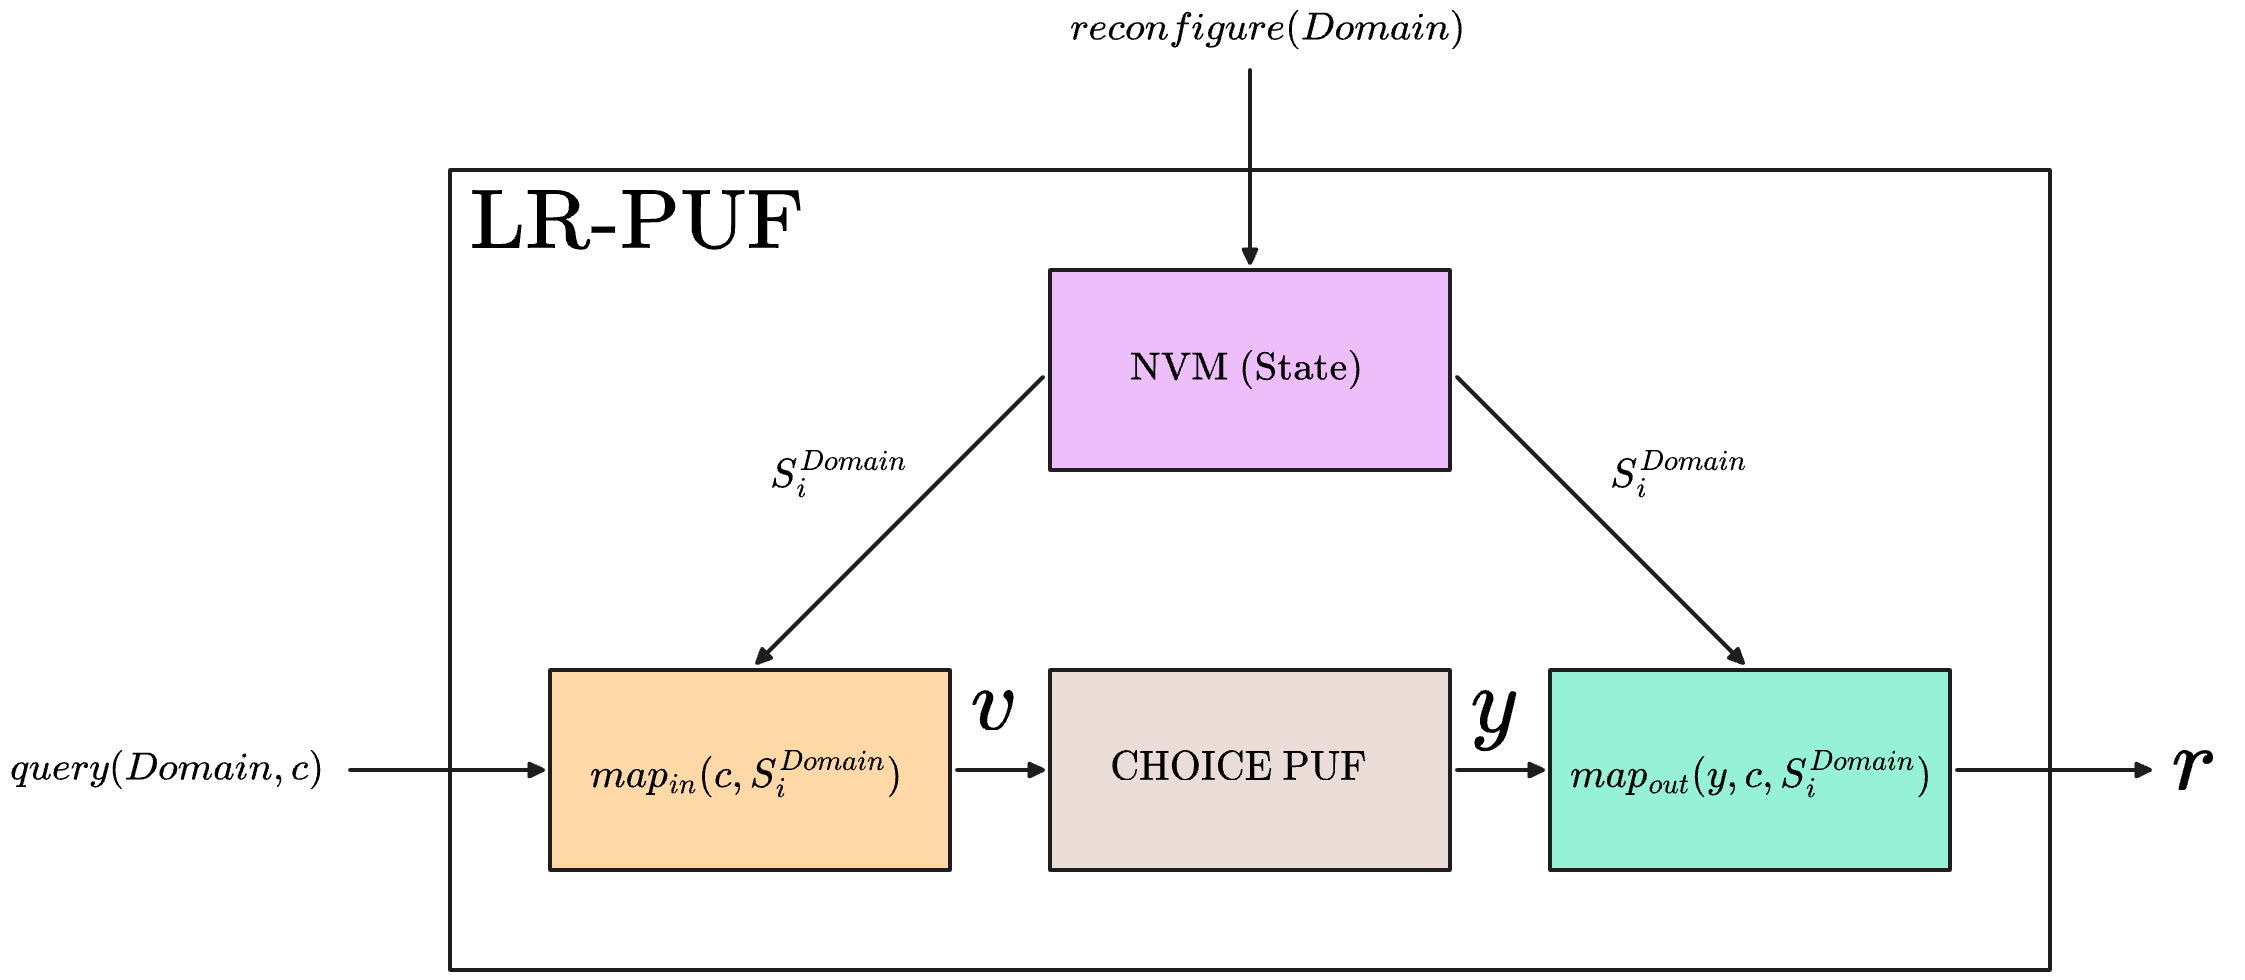
\includegraphics[width=1\linewidth]{img/LR-PUF-Diagram.png}
    \caption{LR-PUF Diagram}
    \label{fig:LR-PUF-Diagram}
\end{figure}

Our chosen LR-PUF architecture can be found in figure \ref{fig:LR-PUF-Diagram}. The LR-PUF augments the CHOICE PUF by using a state that is applied on the incoming challenges through the $map_{in}$ function and on the outgoing responses through the $map_{out}$ function. Calling the $reconfigure$ function changes the state and by extension the CRP behavior of the LR-PUF. Before explaining each of these functions, we need to first clarify the variables shown in the diagram as follows:
\begin{itemize}
    \item $Domain$: We keep a state for each domain or server that the user is connected to. We use the terms server and domain interchangeably.
    \item $S_i^{Domain}$: The current state $i$ associated with some domain. In practice, this state could be any random sequence of bits or integer. It is stored in non-volatile memory, and as per the LR-PUF specification, an attacker with access to this state value cannot use it to uncover the responses of the underlying CHOICE-PUF.
    \item $c$: The outer challenge that is used to query the LR-PUF. As we will see later in the protocol phases, this challenge is to be generated by the server. In practice, it can be any random integer.
    \item $v$: The inner challenge to which the outer challenge $c$ is mapped by calling $v = map_{in}(c, S_i^{Domain})$. This inner challenge is one of the valid challenges uncovered after running the one-time initialization outlined in algorithm \ref{alg:CPUF-one-time-init}. 
    \item $y$: The raw response of the CHOICE-PUF after querying it with challenge $v$.
    \item $r$: The final response of the LR-PUF that will be used as a seed for key generation. It is the result of using the state and $y$ through $r = map_{out}(y, c, S_i^{Domain})$, $c$ is used here to avoid getting the same response twice for the different outer challenges $c_i$ and $c_j$ that would map to the same inner challenge $v$ and give the same response $y$ under some state, because the CHOICE PUF has a limited number of possible challenges and outputs we want to avoid this edge case where two challenges would produce the same response by adding $c$ as input to the $map_{out}$ function.
\end{itemize}

\subsubsection{The $map_{in}$ function}
The input mapping function $map_{in}(c, S_i^{Domain})$ (Algorithm \ref{alg:LRPUF-mapin}) is responsible for translating an arbitrary external challenge $c$ into a valid CHOICE PUF challenge $v \in \mathcal{V}$. It defines a mapping from the set of positive integers $\mathbb{Z}^{+}$ into the set of valid challenges $\mathcal{V}$. The function first derives an index $idx$ by hashing the current domain state with the external challenge and calculating the remainder over the total number of valid challenges to get an index within that range. Then this index is used to select the valid challenge from the set $\mathcal{V}$. This ensures that only valid challenges are used to query the CHOICE PUF and hides the complexity of the CHOICE PUF from the server by allowing it to use any arbitrary challenge $c$. As we will see in a later section explaining the protocol, this challenge $c$ would act similar to a session identifier.

\begin{algorithm}[ht!]
\caption{$map_{in}(c, S_i^{Domain})$}
\begin{algorithmic}[1]
    \Require Challenge $c$, domain state $S_i^{Domain}$, valid challenges set $\mathcal{V}$ stored in NVM
    \Ensure  Mapped challenge $v \in \mathcal{V}$
    \State $idx \leftarrow H(S_i^{Domain} \mathbin\| c) \bmod |\mathcal{V}|$
    \State $v \leftarrow \mathcal{V}[idx]$
    \State \Return $v$
\end{algorithmic}
\label{alg:LRPUF-mapin}
\end{algorithm}

\subsubsection{The $map_{out}$ function}
The output mapping function $map_{out}(y, c, S_i^{Domain})$ (Algorithm \ref{alg:LRPUF-mapout}) is applied on the raw CHOICE PUF response $y$ to produce the final response $r$. It hashes $y$ along with $c$ and the current state $S_i^{Domain}$. Binding $c$ into the output hash prevents response reuse across different challenges since the input space of the CHOICE PUF is quite small and collisions in the $map_{in}$ could happen if queried under the same state.

\begin{algorithm}[ht!]
\caption{$map_{out}(y, c, S_i^{Domain})$}
\begin{algorithmic}[1]
    \Require PUF response $y$, challenge $c$, domain state $S_i^{Domain}$
    \Ensure  Final response $r$
    \State $r \leftarrow H(S_i^{Domain} \mathbin\| c \mathbin\| y)$
    \State \Return $r$
\end{algorithmic}
\label{alg:LRPUF-mapout}
\end{algorithm}

\subsubsection{The $reconfigure$ function}
The reconfiguration function (Algorithm \ref{alg:LRPUF-reconfig}) is the mechanism through which logical reconfigurability is achieved. When called, it generates a random seed using a true random number generator (TRNG) and records the current timestamp. Then it distinguishes between two cases. If no state exists for the given domain, an initial state $S_0^{Domain}$ is derived by selecting a challenge $v$ from  $\mathcal{V}$ using the random seed, then the CHOICE PUF is queried with this challenge $v$ to obtain a response $y$, after which we hash $v$, $y$, the seed and the current timestamp to produce $S_0^{Domain}$. If a state already exists for the given domain, a new state $S_{i+1}^{Domain}$ is derived by hashing the current state $S_i^{Domain}$ with the random seed and timestamp, forming a hash chain that evolves the current state. In both cases, the produced state is finally persisted into the NVM to be used in subsequent LR-PUF querying operations.

\begin{algorithm}[ht!]
\caption{$reconfigure(Domain)$}
\begin{algorithmic}[1]
    \Require Domain identifier $Domain$, valid challenges set $\mathcal{V}$ stored in NVM
    \Ensure  NVM updated with new domain state $S_{i+1}^{Domain}$

    \State $S_i^{Domain} \leftarrow NVM.read(Domain)$
    \State $seed \leftarrow TRNG()$
    \State $now \leftarrow readtime()$

    \If{$S_i^{Domain} = null$} \Comment{Initialize the first state for a new domain}
        \State $idx \leftarrow seed \bmod |\mathcal{V}|$
        \State $v \leftarrow \mathcal{V}[idx]$
        \State $y \leftarrow CHOICE\_PUF(v)$
        \State $S_0^{Domain} \leftarrow H(v \mathbin\| y \mathbin\| seed \mathbin\| now)$
        \State $NVM.write(Domain,S_0^{Domain})$
    \Else
        \State $S_{i+1}^{Domain} \leftarrow H(S_{i}^{Domain} \mathbin\| seed \mathbin\| now)$ 
        \State $NVM.write(Domain,S_{i+1}^{Domain})$
    \EndIf
\end{algorithmic}
\label{alg:LRPUF-reconfig}
\end{algorithm}

\subsubsection{The $query$ function}
The query operation (Algorithm \ref{alg:LRPUF-query}) takes a challenge $c$ and a domain identifier $Domain$. It first retrieves the current domain state $S_i^{Domain}$ associated with the given domain from NVM. Then $c$ is passed along with $S_i^{Domain}$ to $map_{in}$ to get a valid challenge $v$. After that, $v$ is used to query the CHOICE PUF and get a response $y$. Finally $y$ is passed to the $map_{out}$ function along with $c$ and $S_i^{Domain}$ to produce the final response $r$.

\begin{algorithm}[ht!]
\caption{$query(c,Domain)$}
\begin{algorithmic}[1]
    \Require Domain identifier $Domain$, challenge $c$
    \Ensure  Response $r$ 
    \State $S_i^{Domain} \leftarrow NVM.read(Domain)$
    \State $v \leftarrow map_{in}(c, S_i^{Domain})$
    \State $y \leftarrow \textsc{CHOICE\_PUF}(v)$
    \State $r \leftarrow map_{out}(y,c, S_i^{Domain})$
    
    \State \Return $r$
\end{algorithmic}
\label{alg:LRPUF-query}
\end{algorithm}

The binding of both mapping functions to the domain state is what enables logical reconfigurability. By invoking $reconfigure(Domain)$, the state is updated, causing all subsequent queries to the LR-PUF under the same domain to produce entirely different responses without any modifications to the underlying weak CHOICE PUF. 

\subsection{Error Correction Strategy}

Since the outputs of the CHOICE PUF can be noisy, a robust error correction strategy is needed. A fuzzy commitment scheme utilizing a BCH code \cite{BOSE196068} was used.

A BCH code is a cyclic error-correction code parameterized by a codeword length $n$, a message length $k$, and a correction capacity $t$. Given a $k$-bit message $W$, $encode_{BCH}(W)$ appends $(n - k)$ parity bits stored as $ECC$, where $W||ECC$ make up the codeword. During decoding, $decode_{BCH}(W', ECC)$ uses those parity bits to locate and correct up to $t$ bit flips in the noisy word $W'$ and obtain the original $W$.



The error correction strategy for the LR-PUF involves two operations: enrollment and querying. 
\subsubsection{Enrollment}
The enrollment operation is described with the $enroll_{BCH}$ function (Algorithm \ref{alg:PUF-BCH-Enroll}). This is what is actually used to generate a key using the LR-PUF. At first, it takes as input the $Domain$, the outer challenge $c$ and how many times $vote\_count$ to query the CHOICE-PUF to determine a stable response using bit-wise majority voting. Since this enrollment process usually occurs when we want to generate a key for the first time or when we want to rotate keys, the $reconfigure$ function must run to ensure that we have a new state $S_i^{Domain}$. Then this state is used to map the outer challenge $c$ to a valid inner challenge $v$ using the $map_{in}$ function. This challenge $v$ is used to query the CHOICE PUF $vote\_count$ times to determine using bit-wise majority voting the stable PUF response $y$. After this, a secret value $W$ is generated by hashing the state $S_i^{Domain}$, the outer challenge $c$, the PUF response $y$ and the current timestamp. This $W$ value is what will be error-corrected as part of the fuzzy commitment scheme. It was generated this way to make sure that it is sufficiently random. Then $W$ is encoded using BCH error correction to produce the parity bits $ECC$, which are stored in NVM. Helper data $helper = y \oplus W$ is also stored. This is done so that during querying, a noisy PUF response $y'$ can be XORed with $helper$ to recover a noisy version of $W$ which $ECC$ can correct. Finally, $W$ is given to the $map_{out}$ function along with the outer challenge $c$ and the current state $S_i^{Domain}$ to obtain the final response $r$ which can be used as a seed for key generation.

\begin{algorithm}[ht!]
\caption{$enroll_{BCH}(Domain, c, vote\_count)$}
\begin{algorithmic}[1]
    \Require Domain identifier $Domain$, challenge $c$, bit-wise majority voting count $vote\_count$
    \Ensure  Response $r$ (seed) 
    \State $reconfigure(Domain)$
    \State $S_i^{Domain} \leftarrow NVM.read(Domain)$
    \State $v \leftarrow map_{in}(c, S_i^{Domain})$
    \State \(\triangleright\) Bit-wise majority voting to determine the CHOICE PUF response $y$
 \State $\text{ones}[0..63] \leftarrow \mathbf{0}$
  \For{$i = 1$ \textbf{to} $vote\_count$}
      \State $m \leftarrow \textsc{CHOICE\_PUF}(v)$
      \For{$b = 0$ \textbf{to} $63$}
          \State $\text{ones}[b] \leftarrow \text{ones}[b] + m[b]$
      \EndFor
  \EndFor
 \For{$b = 0$ \textbf{to} $63$}
      \If{$\text{ones}[b] \cdot 2 \geq vote\_count$}
          \State $y[b] \leftarrow 1$
      \Else
          \State $y[b] \leftarrow 0$
      \EndIf
  \EndFor
    \State \(\triangleright\) Fuzzy commitment
    \State $W \leftarrow H(S_i^{Domain}||c||y||now)$
    \State $ECC \leftarrow encode_{BCH}(W)$
    \State $helper \leftarrow y \oplus W$
    \State $NVM.write(Domain, ECC)$
    \State $NVM.write(Domain, helper)$
    \State $r \leftarrow map_{out}(W,c, S_i^{Domain})$ 
    \State \Return $r$
\end{algorithmic}
\label{alg:PUF-BCH-Enroll}
\end{algorithm}



\subsubsection{Querying}
The query operation is described with the $query_{BCH}$ function  (Algorithm \ref{alg:PUF-BCH-Query}). It takes as input the domain identifier $Domain$ and the outer challenge $c$. To recover the response $r$ generated with $enroll_{BCH}$, we first fetch $S_i^{Domain}$, $helper$ and $ECC$ from NVM using $Domain$. Then, $map_{in}$ is used to get the valid challenge $v$ using $c$ and $S_i^{Domain}$. This valid challenge $v$ is used to query the CHOICE PUF once to get a response $y'$. Unlike enrollment, no majority voting is performed here, so $y'$ may be noisy. $W'$ is obtained by taking $y' \oplus helper$, and $decode_{BCH}(W', ECC)$ corrects the errors to recover the original $W$, given that the noise is within the error-correction capacity of the BCH code. Finally, $W$ is given to $map_{out}$ along with $c$ and $S_i^{Domain}$ to obtain the original $r$ so that we can use it as a seed to recover the previously enrolled key.



\begin{algorithm}[ht!]
\caption{$query_{BCH}(Domain, c)$}
\begin{algorithmic}[1]
    \Require Domain identifier $Domain$, challenge $c$.
    \Ensure  Response $r$ (seed) 
    \State $S_i^{Domain},helper,ECC \leftarrow NVM.read(Domain)$
    \State $v \leftarrow map_{in}(c, S_i^{Domain})$
    \State $y' \leftarrow CHOICE\_PUF(v)$
    \State $W' \leftarrow y' \oplus helper $
    \State $W \leftarrow decode_{BCH}(W', ECC)$
    \State $r \leftarrow map_{out}(W,c, S_i^{Domain})$ 
    \State \Return $r$
\end{algorithmic}
\label{alg:PUF-BCH-Query}
\end{algorithm}

\subsection{Justifications for using a PUF}
Since the question of "Why use a PUF specifically and not some other conventional secure storage primitive?" is one that will be asked when looking at the dongle design, an answer is in order. The design choice to use a PUF rather than some other secure storage primitive, like a TPM or encrypted flash memory, is a deliberate one. Although these other mechanisms are mature, standardized and widely deployed, they all share one common property: the secret physically resides somewhere on the die at all times. The PUF approach does not have this property. This allows it to provide several benefits that align with REPUSH's threat model and design goals.

First, there is no key at rest. The private key is generated on demand and discarded immediately after use. An attacker that obtains a powered-off dongle finds no secret to extract. Although physical attacks are out of scope for our threat model, this property could be useful in future iterations of the REPUSH protocol that would consider physical attacks as well.

Second, there is no key provisioning step needed to be taken by the manufacturer. Other schemes, where a key is stored, introduce a trust dependency on the supply chain of the dongle. With a PUF, the cryptographic identity emerges from the chip fabric itself without requiring explicit introduction of the secret by some manufacturer.

The second benefit is more in line with REPUSH's security goals as we are trying to reduce the dependency on third parties and also makes more sense economically since no provisioning step is needed for manufacturing the dongles.

\section{Protocol Design}
The REPUSH protocol is composed of three phases.
The following notations are used: $\{m\}_K$ denotes encryption of $m$ with key $K$, $[m]_K$ denotes a signature on $m$ with key $K$,
and $||$ is concatenation. The steps shown as $\boldsymbol{\langle x \rangle}$ may fail, in which case the red arrow branch is taken.
The diagrams contain a high-level overview of the process, each function is described in more detail in its respective algorithm figure. In the algorithms pseudo-code, querying the LR-PUF is indicated with $query_{BCH}(Challenge, Domain)$ (Algorithm \ref{alg:PUF-BCH-Query}).

\subsection{Phase 1: Enrollment and Login}
The first phase of REPUSH initiates a session between the dongle and the server. This phase has two objectives:
\begin{enumerate}
    \item Mutual authentication by authenticating the server to the dongle and user using a CA certificate, and then authenticating the user and the dongle to the server with a username and password. 
    \item Establishing a dongle-bound asymmetric key pair $SK_0$ and $PK_0$ to be used for the first session.
\end{enumerate}

\begin{figure}
    \centering
    \includegraphics[width=1.25\linewidth]{img/REPUSH-1.png}
    \caption{Phase 1: Enrollment and Login}
    \label{fig:REPUSH-phase-1}
\end{figure}

The first phase described in figure \ref{fig:REPUSH-phase-1} is composed of the following steps:
\paragraph{$\boldsymbol{(1)}$} The user initiates a dongle login request with the server using the browser. As opposed to a normal login request, the dongle login request tells the browser that the user wants to associate a dongle with the session.

\paragraph{$\boldsymbol{(2)}$} Consequently, the server runs the function $DongleLogin()$ (Algorithm \ref{alg:dongle-login}) to fetch the $Cert$ and generate a $LoginPayload$. The $Cert$ associates the server's $Domain$ with its public key $PK_{Server}$ using a signature signed by the CA, the dongle will later use this $Cert$ to authenticate the server. The $LoginPayload$ is also intended for the dongle, it contains the following:
\begin{itemize}
    \item The string \verb|"login"| that will tell the dongle to perform a login operation.
    \item A randomly generated challenge for the LR-PUF $C_\text{Session}^0$ that will be used by the dongle to generate the asymmetric key pair $(SK_0,PK_0)$ for the first session.
    \item A nonce $N$ to avoid playback attacks and to track the requests.
    \item A login payload composed of a signature on $\verb|"login"|||C_\text{Session}^0||N$ with $SK_\text{Server}$ to prove to the dongle that this payload is indeed coming from the expected domain or server.
\end{itemize}
\begin{algorithm}[ht!]
\caption{$DongleLogin()$}
\begin{algorithmic}[1]
    \Require Incoming dongle login request
    \Ensure  $(\mathit{Cert}, \mathit{LoginPayload})$ returned to the browser.

    \State $C^0_{\text{Session}} \leftarrow TRNG()$
    \State $N \leftarrow TRNG()$
    \State $Cert \leftarrow (Domain||PK_\text{Server},[Domain||PK_\text{Server}]_{SK_{CA}})$
    \State $\mathit{LoginPayload} \leftarrow
            (\texttt{"login"} || C^0_{\text{Session}} || N,
            [\texttt{"login"} || C^0_{\text{Session}} || N]_{\mathit{SK}_{\text{Server}}})$
    \State \textbf{return} $(\mathit{Cert}, \mathit{LoginPayload})$
\end{algorithmic}
\label{alg:dongle-login}
\end{algorithm}
\paragraph{$\boldsymbol{(3)}$} The server sends back $Cert$ and $LoginPayload$ to the browser, then the browser forwards them to DOMAN (via HTTP).
\paragraph{$\boldsymbol{(4)}$} DOMAN sends an "Enroll" request to the dongle (via a Serial interface) for the dongle to run the $DongleEnroll(Cert, LoginPayload)$ function (Algorithm \ref{alg:dongle-enroll}).

\begin{algorithm}[ht!]
\caption{$DongleEnroll(Cert, LoginPayload)$}
\begin{algorithmic}[1]
    \Require Enroll command with $(\mathit{Cert}, \mathit{LoginPayload})$ received from the DOMAN.
    \Ensure  $(\mathit{LoginToken}, Domain, \mathit{SignedPayload})$ returned to the browser,
             or an error.

    \State $V_{\text{Server}} \leftarrow Verify(Cert, PK_{CA})$
    \If{$V_{\text{Server}} = \text{failed}$}
        \State \textbf{return} "Certificate verification failed"
    \EndIf
    \State $Domain, PK_{\text{Server}} \leftarrow Cert$
    \State $V_{\text{Payload}} \leftarrow Verify(LoginPayload, PK_{\text{Server}})$
    \If{$V_{\text{Payload}} = \text{failed}$}
        \State \textbf{return} "Payload verification failed"
    \EndIf
    \State $P, Username, Password \leftarrow UserLogin(Domain)$
    \If{$P = \text{reject}$}
        \State \textbf{return} "User rejected login request"
    \EndIf
%    \State $reconfigure(Domain)$ \Comment{Initializes $S_0^{Domain}$}
    \State $C^0_{\text{Session}} \leftarrow LoginPayload$
    \State $seed_0 \leftarrow enroll_{BCH}(Domain, C^0_{\text{Session}}, 10)$
    \State $SK_0, PK_0 \leftarrow KeyGen(seed_0)$
    \State $LoginToken \leftarrow \{Username||Password||PK_0\}_{PK_{\text{Server}}}$
    \State $SignedLoginPayload \leftarrow [LoginPayload]_{SK_0}$
    \State \textbf{return} $(LoginToken, Domain, SignedLoginPayload)$
\end{algorithmic}
\label{alg:dongle-enroll}
\end{algorithm}
\paragraph{$\boldsymbol{\langle 5\rangle}$} The dongle first verifies if the provided $Cert$ was actually signed by the $CA$, if this step fails, the login request is rejected by the dongle.
\paragraph{$\boldsymbol{\langle 6\rangle}$} The dongle extracts $PK_\text{Server}$ from $Cert$ and uses it to verify if the signed $LoginPayload$ is indeed coming from the server. If this step fails, the login request is rejected by the dongle.
\paragraph{$\boldsymbol{\langle 7\rangle}$} The $Domain$ extracted from $Cert$ is displayed on the dongle's touch screen (Figure \ref{fig:login-screens}), where the user is expected to read it and verify if it is the intended domain where they wish to login. The user has two options, either to accept or reject this login request. This here concludes the part where the dongle authenticates the server. The displayed $Domain$ was extracted from $Cert$ and is guaranteed to actually be associated with $PK_\text{Server}$ because of the CA's signature on it. Furthermore, if a compromised host tries fooling the dongle with some other $Domain$ here, the user will catch on because the $Domain$ is displayed on the screen and requires approval. 
\paragraph{$\boldsymbol{\langle 8\rangle}$} The user is prompted to enter their $Username$ and $Password$ for the $Domain$ on the dongle's touch screen (Figure \ref{fig:login-screens}). Alternatively, the dongle could be used as a password manager in this step to make it more practical for the user so that they do not have to manually enter their credentials every time, but this use-case is currently out of scope for REPUSH's focus on protecting against session hijacking. The user can still cancel at this point, in which case the login request is rejected by the dongle.
\begin{figure}
    \centering
    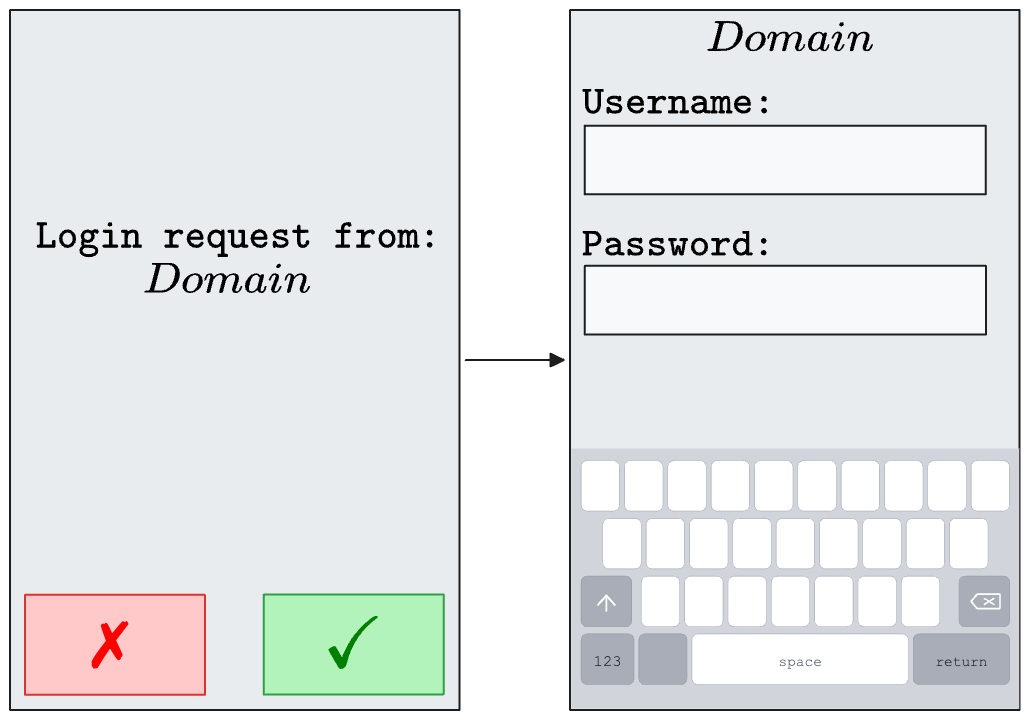
\includegraphics[width=0.5\linewidth]{img/touch-screen-login.png}
    \caption{User prompts for login on the dongle's touch screen}
    \label{fig:login-screens}
\end{figure}
\paragraph{$\boldsymbol{(9)}$} The LR-PUF is queried using $C_\text{Session}^0$ to generate the key pair $(SK_0, PK_0)$, this is done by first running $enroll_{BCH}(Domain, C_\text{Session}^0,10)$ (Algorithm \ref{alg:PUF-BCH-Enroll}) which will in turn initialize $S_0^{Domain}$ and perform the necessary error-encoding to get as a response $seed_0$, this seed is then given to some key generation algorithm to get an asymmetric key pair $(SK_0, PK_0)$.
\paragraph{$\boldsymbol{(10)}$} The user-provided $Username$ and $Password$ along with the generated public key $PK_0$ are encrypted using the server public key $PK_\text{Server}$ to create $LoginToken$. This $LoginToken$ is encrypted with $PK_\text{Server}$ to ensure that only the server can decrypt it and access the user's password within.
\paragraph{$\boldsymbol{(11)}$} The provided $LoginPayload$ is signed with $SK_0$ to further confirm to the server that the dongle did in fact receive the $LoginPayload$ and the $PK_0$ can be used for the first session.
\paragraph{$\boldsymbol{(12)}$} $LoginToken$, $Domain$ and $[LoginPayload]_{SK_0}$ are returned to DOMAN, then DOMAN sends them to the browser, and finally the browser sends $LoginToken$ and $[LoginPayload]_{SK_0}$ to the server. The server then runs the function $VerifyLogin(LoginToken, [LoginPayload]_{SK_0})$ (Algorithm \ref{alg:verify-login}).

\begin{algorithm}[ht!]
\caption{$VerifyLogin(LoginToken, [LoginPayload]_{SK_0})$}
\begin{algorithmic}[1]
    \Require $LoginToken$ and $[LoginPayload]_{SK_0}$.
    \Ensure  $LoginAck$ and session $Cookies_0$ returned to the browser,
             or an error.

    \State $D_{LoginToken} \leftarrow Decrypt(LoginToken, SK_{\text{Server}})$
    \If{$D_{LoginToken} = \text{failed}$}
        \State \textbf{return} "Reject login request"
    \EndIf
    \State $Username, Password, PK_0 \leftarrow D_{LoginToken}$
    \State $auth \leftarrow Authenticate(Username, Password)$ \Comment{optional: extra MFA}
    \If{$auth = \text{failed}$}
        \State \textbf{return} "Reject login request"
    \EndIf
    \State $V_{Payload} \leftarrow Verify(SignedPayload, PK_0)$
    \If{$V_{Payload} = \text{failed}$}
        \State \textbf{return} "Reject login request"
    \EndIf
    \State $LoginAck \leftarrow [PK_0||C_{Session}^0||Domain]_{SK_{\text{Server}}}$
    \State $store(PK_0,\ C^0_{\text{Session}})$
    \State $Cookies_0 \leftarrow GenerateCookies()$
    \State $t^{Session}_{\text{last}} \leftarrow Now()$ 
    \State $t^{Session}_{\text{start}} \leftarrow Now()$
    \State \textbf{return} $(LoginAck, Cookies_0)$
\end{algorithmic}
\label{alg:verify-login}
\end{algorithm}

\paragraph{$\boldsymbol{\langle 13\rangle}$ and $\boldsymbol{\langle 14\rangle}$} The server decrypts $LoginToken$ using $SK_\text{Server}$ to get $Username$, $Password$ and $PK_0$ from it. If one of these steps fails, the login request is rejected.
\paragraph{$\boldsymbol{\langle15\rangle}$} The server checks the validity of the provided $Username$ and $Password$ against its internal database, optionally, an extra multi-factor authentication step could be added here for extra security. If this step fails, the login request is rejected.
\paragraph{$\boldsymbol{\langle16\rangle}$} $[LoginPayload]_{SK_0}$ is verified using $PK_0$ for the server to verify that $LoginPayload$ was indeed received and signed by the dongle and that $PK_0$ has been agreed as the first key for this session. If this step fails, the login request is rejected.
\paragraph{$\boldsymbol{(17)}$} A login acknowledgment $LoginAck$ is created by signing $PK_0||C_{Session}^0||Domain$ with $SK_\text{Server}$. This login acknowledgment will later be sent to the dongle to acknowledge the login.
\paragraph{$\boldsymbol{(18)}$} A session is created by associating $PK_0$ with $C_{Session}^0$ and generating $Cookies$. 
\paragraph{$\boldsymbol{(19)}$} $Cookies$ and $LoginAck$ are sent to the browser.
\paragraph{$\boldsymbol{(20)}$} $Cookies$ stay in the browser, and $LoginAck$ and $Domain$ are sent to the dongle for it to run $AckEnroll(Domain, LoginAck)$ (Algorithm \ref{alg:ack-enroll}).
\begin{algorithm}[ht!]
\caption{$AckEnroll(Domain, LoginAck)$}
\begin{algorithmic}[1]
    \Require $(Domain, LoginAck)$ received from the browser.
    \Ensure  Login success on valid acknowledgment returned to the browser and persisted state
             $(Domain, S_0^{Domain}, C^0_{\text{Session}}, PK_0)$ in the dongle. Otherwise, a login error is returned to the browser.
     \State $V_{LoginAck} \leftarrow Verify(LoginAck, PK_0||C^0_{\text{Session}}||Domain, PK_{\text{Server}})$
    \If{$V_{LoginAck} = \text{failed}$}
        \State \textbf{return} "Login not acknowledged"
    \EndIf
    \State $store(Domain, S_0^{Domain}, C^0_{\text{Session}}, PK_0)$
    \State \textbf{return} "Login success"
\end{algorithmic}
\label{alg:ack-enroll}
\end{algorithm}
\paragraph{$\boldsymbol{\langle21\rangle}$} The signature $LoginAck$ is verified using $PK_{Server}$ and the already established $PK_0$, $C_{Session}^0$ and $Domain$. If this step fails a login error is returned to the browser.
\paragraph{$\boldsymbol{(22)}$} The tuple $(Domain, S_0^{Domain}, C^0_{\text{Session}}, PK_0)$ is stored on the dongle for it to be used in the next phase of the protocol.

\paragraph{$\boldsymbol{(23)}$} On login success returned from the dongle, the tuple $(Domain, Cookies)$ is stored on the browser.

By the end of this first phase, we would have securely established $PK_{Server}$ on the dongle thanks to the CA certificate, and $PK_0$ on the server-side with the $LoginToken$ which associates $Username$ and $Password$ with $PK_0$. The dongle used $Cert$ as trust anchor, whilst the server used the user's credentials as a trust anchor for accepting $PK_0$. We will now see in the next phase of the protocol how $PK_0$ or any subsequent $PK_i$ can be used for continuous session validation.

\subsection{Phase 2: Operation Phase}
The operation phase has two concurrent modes of operation, the first is similar to PUSH's approach to continuous session validation, where requests are allowed as long as the cookies are provided for a certain validity window, after which the dongle is requested to sign a nonce with $SK_i$ given $C_{Session}^i$ to prove ownership of the dongle. REPUSH adopts this approach for non-sensitive requests. For sensitive requests, the second mode of operation is in order. In which the request must be approved by the user on the dongle's screen and then signed with $SK_i$. 
\subsubsection{Non-sensitive Requests Operation}
What counts as "non-sensitive" is a judgment to be made by the server or application. For example, read-only navigation, pagination, search queries and fetching static content can be considered as "non-sensitive". 

\begin{figure}
    \centering
    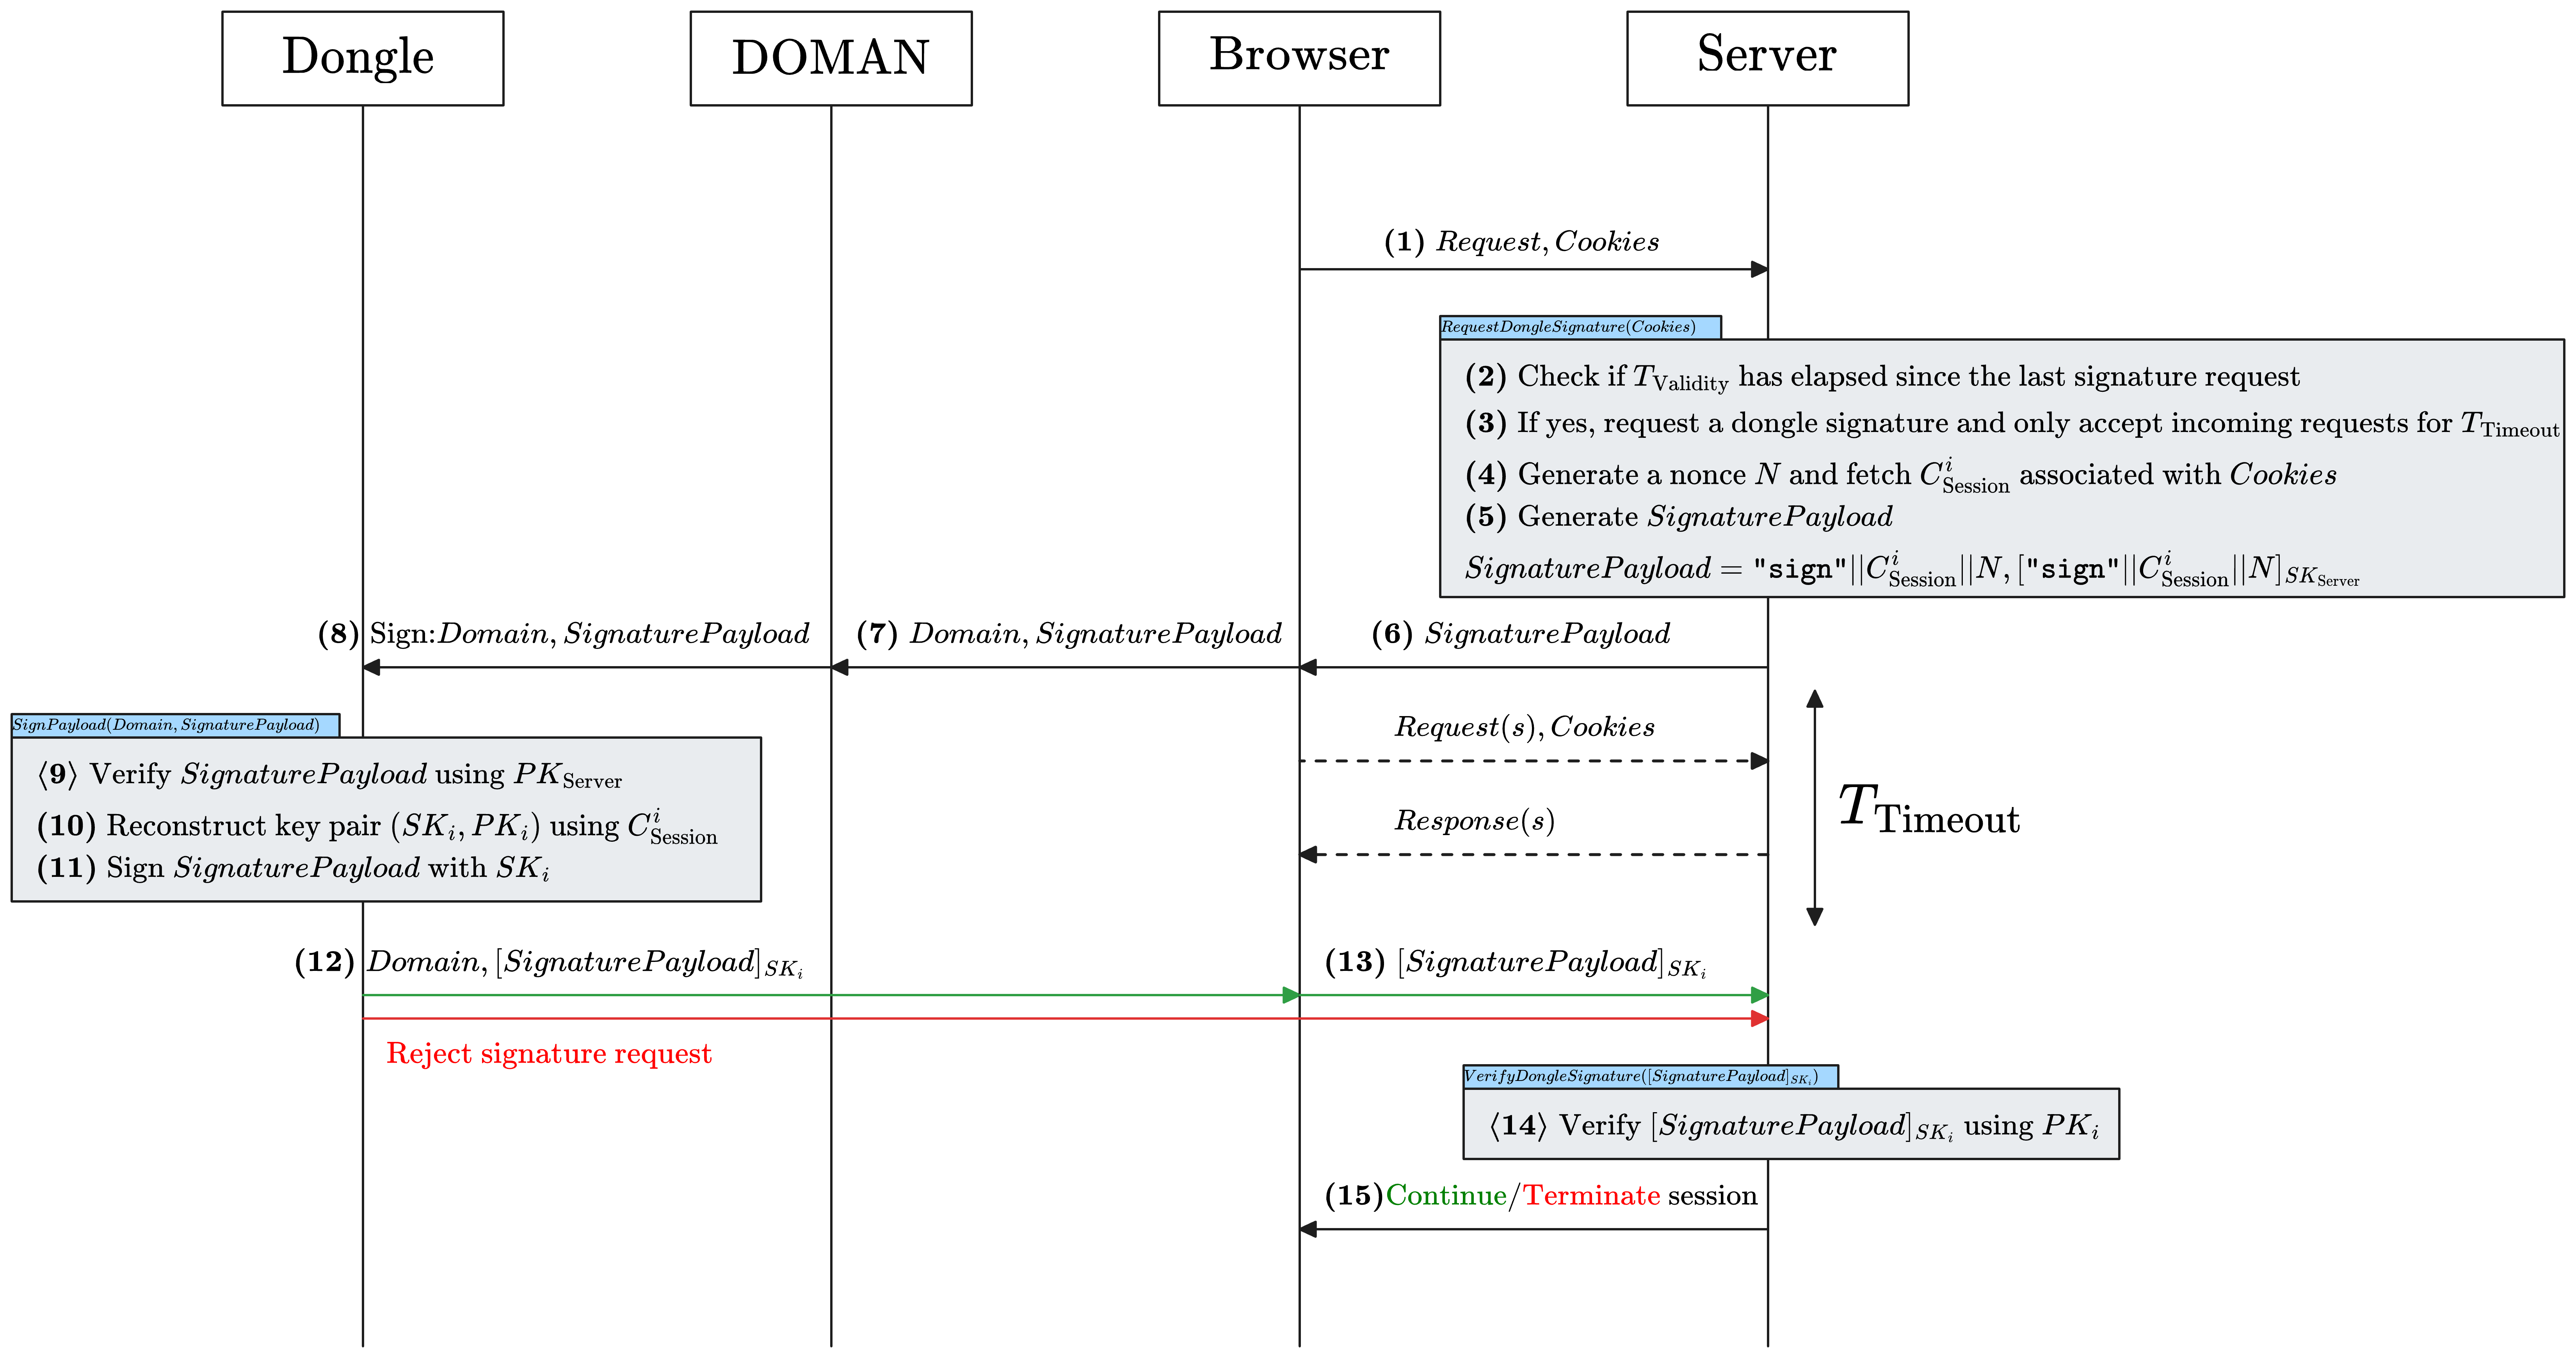
\includegraphics[width=1.25\linewidth]{img/REPUSH-2-Non-Sensitive.png}
    \caption{Phase 2: Operation Phase - Non-sensitive Requests}
    \label{fig:REPUSH-phase-2-non-sensitive}
\end{figure}

The continuous session validation for non-sensitive requests is defined in Figure \ref{fig:REPUSH-phase-2-non-sensitive}. Here the following time variables are used to determine session validity and when to request proof of dongle ownership:
\begin{itemize}
    \item $T_\text{Validity}$: The maximum time interval within which the server accepts incoming requests without a fresh dongle signature. The smaller this interval, the sooner a hijacked session is caught, but at the cost of more latency.
    \item $T_\text{Timeout}$: The grace time window within which the server accepts incoming requests after requesting a fresh dongle signature. If no valid signature arrives by the end of this time window, the session is terminated.
    \item $t^{Session}_{\text{last}}$: The timestamp of the last successful dongle validation for the current session, it is initialized as $Now()$ when Phase 1 completes. 
    \item $t^{Session}_\text{deadline}$: The timestamp deadline by which the currently requested dongle signature must arrive, it is set to $Now() + T_\text{Timeout}$ when a dongle signature is requested. 
\end{itemize}

This phase is composed of the following steps: 

\paragraph{$\boldsymbol{(1)}$} The browser makes some request to the server and presents the $Cookies$ along. On every request received, the server will run the function $RequestDongleSignature(Cookies)$ (Algorithm \ref{alg:request-dongle-signature}). 
\begin{algorithm}[ht!]
\caption{$RequestDongleSignature(Cookies)$}
\begin{algorithmic}[1]
    \Require Incoming request with $Cookies$, and
             per-session state including $t^{Session}_{\text{last}}$ and $C^i_{\text{Session}}$.
    \Ensure  $SignaturePayload$ returned to the browser when revalidation is due;
             otherwise the request is served normally.
    \State $\Delta_\text{Elapsed} \leftarrow Now() - t^{Session}_{\text{last}}$
    \If{$\Delta_\text{Elapsed} < T_{\text{Validity}}$}
        \State \textbf{return} \texttt{NULL} \Comment{still within the validity window}
    \EndIf
    \State $t^{Session}_{\text{deadline}} \leftarrow Now() + T_{\text{Timeout}}$
    \State $N \leftarrow TRNG()$
    \State $C^i_{\text{Session}} \leftarrow Fetch(Cookies)$
    \State $SignaturePayload \leftarrow
            (\texttt{"sign"} || C^i_{\text{Session}} || N,
            [\texttt{"sign"} || C^i_{\text{Session}} || N]_{SK_{\text{Server}}})$
    \State $TriggerTerminateOn(t_\text{deadline}^{Session})$
    \State \textbf{return} $SignaturePayload$
\end{algorithmic}
\label{alg:request-dongle-signature}
\end{algorithm}
\paragraph{$\boldsymbol{(2)}$ and $\boldsymbol{(3)}$} Before processing the request, the server checks if $T_\text{Validity}$ has elapsed since the last signature by checking if $Now() - t_\text{last}^{Session} < T_\text{Validity}$. If this condition is true, then no verification is needed for now and the request is processed. Otherwise, $t_\text{deadline}^{Session}$ is set to $Now() + T_\text{Timeout}$, a signature is requested from the dongle and requests continue to be served up to $t_\text{deadline}^{Session}$.
\paragraph{$\boldsymbol{(4)}$ and $\boldsymbol{(5)}$} To request a signature from the dongle, a nonce $N$ is generated and the challenge $C_\text{Session}^i$ associated with the cookies is fetched to generate $SignaturePayload = (\texttt{"sign"} || C^i_{\text{Session}} || N,
            [\texttt{"sign"} || C^i_{\text{Session}} || N]_{SK_{\text{Server}}})$. Then a trigger on the server is started which will terminate the session when the timestamp reaches $t_\text{deadline}^{Session}$.
\paragraph{$\boldsymbol{(6)}$, $\boldsymbol{(7)}$ and $\boldsymbol{(8)}$} $SignaturePayload$ is sent to the browser. Then the browser sends $Domain$ and $SignaturePayload$ to DOMAN, which then forwards it to the dongle as a signature request to run the function $SignPayload(Domain, SignaturePayload)$ (Algorithm \ref{alg:sign-payload}) 
\begin{algorithm}[ht!]
\caption{$SignPayload(Domain, SignaturePayload)$}
\begin{algorithmic}[1]
    \Require $(Domain, SignaturePayload)$ received from DOMAN.
    \Ensure  $(Domain, [SignaturePayload]_{SK_i})$ returned to the browser, or an error.
    \State $V_{Payload} \leftarrow Verify(SignaturePayload, PK_{\text{Server}})$
    \If{$V_{Payload} = \text{failed}$}
        \State \textbf{return} ``Reject signature request''
    \EndIf
    \State $\texttt{"sign"},\ C^i_{\text{Session}},\ N \leftarrow SignaturePayload$
%    \State $seed'_i \leftarrow LR\text{-}PUF(S_i^{Domain},\ C^i_{\text{Session}})$
%    \State $seed_i \leftarrow ErrorCorrect(seed'_i)$
    \State $seed_i \leftarrow query_{BCH}(Domain, C^i_\text{Session})$ 
    \State $SK_i,\ PK_i \leftarrow KeyGen(seed_i)$
    \State $[SignaturePayload]_{SK_i} \leftarrow Sign(SignaturePayload, SK_i)$
    \State \textbf{return} $(Domain, [SignaturePayload]_{SK_i})$
\end{algorithmic}
\label{alg:sign-payload}
\end{algorithm}

\paragraph{$\boldsymbol{\langle9\rangle}$} Verify the received $SignaturePayload$ using $PK_\text{Server}$ to make sure that the signature request is coming from the server.

\paragraph{$\boldsymbol{(10)}$} Query the LR-PUF with the $query_{BCH}$ (Algorithm \ref{alg:PUF-BCH-Query}) using the challenge $C_\text{Session}^i$ found within $SignaturePayload$ and $Domain$ to get as a response $seed_i$. Here $seed_i$ was actually error-corrected, so it is identical to the one enrolled in the first phase. Then $KeyGen(seed_i)$ is used to generate the key pair $(SK_i, PK_i)$.

\paragraph{$\boldsymbol{(11)}$} Sign $SignaturePayload$ with $SK_i$ to prove to the server that the dongle possesses the private key $SK_i$ associated with the currently enrolled session public key $PK_i$.

\paragraph{$\boldsymbol{(12)}$ and $\boldsymbol{(13)}$} $Domain$ and $[SignaturePayload]_{SK_i}$ is sent to the browser. Then the browser sends $[SignaturePayload]_{SK_i}$ as a response to the server to prove ownership of the dongle. When received, the server will run the function $VerifyDongleSignature([SignaturePayload]_{SK_i})$ (Algorithm \ref{alg:verify-dongle-signature}).

\begin{algorithm}[ht!]
\caption{$VerifyDongleSignature([SignaturePayload]_{SK_i})$}
\begin{algorithmic}[1]
    \Require Signed payload received from the browser, and
             $PK_i$ and $t^{Session}_{\text{deadline}}$ stored in the session state.
    \Ensure  Session continues on valid and timely signature, otherwise it is terminated.
    \State $V \leftarrow Verify([SignaturePayload]_{SK_i}, SignaturePayload, PK_i)$
    \If{$V = \text{failed}$}
        \State $Terminate(Session)$
        \State \textbf{return} "Terminate session"
    \EndIf
    \State $CancelTerminateOn(t_\text{deadline}^{Session})$
    \State $t^{Session}_{\text{last}} \leftarrow Now()$
    \State \textbf{return} "Continue session"
\end{algorithmic}
\label{alg:verify-dongle-signature}
\end{algorithm}

\paragraph{$\boldsymbol{\langle14\rangle}$} The server verifies $[SignaturePayload]_{SK_i}$ using $PK_i$, and $t^{Session}_\text{last}$ is reset to $Now()$ and the termination trigger on $t_\text{deadline}^{Session}$ is canceled.

\paragraph{$\boldsymbol{(15)}$} The session is terminated if the verification of the received signed payload fails or if the timestamp $t_\text{deadline}^{Session}$ is reached before receiving a valid $[SignaturePayload]_{SK_i}$. Otherwise, the session stays alive. Since $SignaturePayload$ is embedded in the server's response to an active request, every connection presenting the stolen cookies independently receives it and must produce a valid signature on it to keep the session attached to that connection. In other words, a cookie or session can be associated with multiple connections, and each connection must prove ownership of the dongle independently to keep the session attached to it. This is to counter the case where an attacker with stolen cookies would rely on the legitimate verification coming from the user to keep the attacker's session alive. This approach also provides a way to handle normal IP changes caused by the ISP that can happen during a session. 

\subsubsection{Sensitive Request Operation}

\begin{figure}
    \centering
    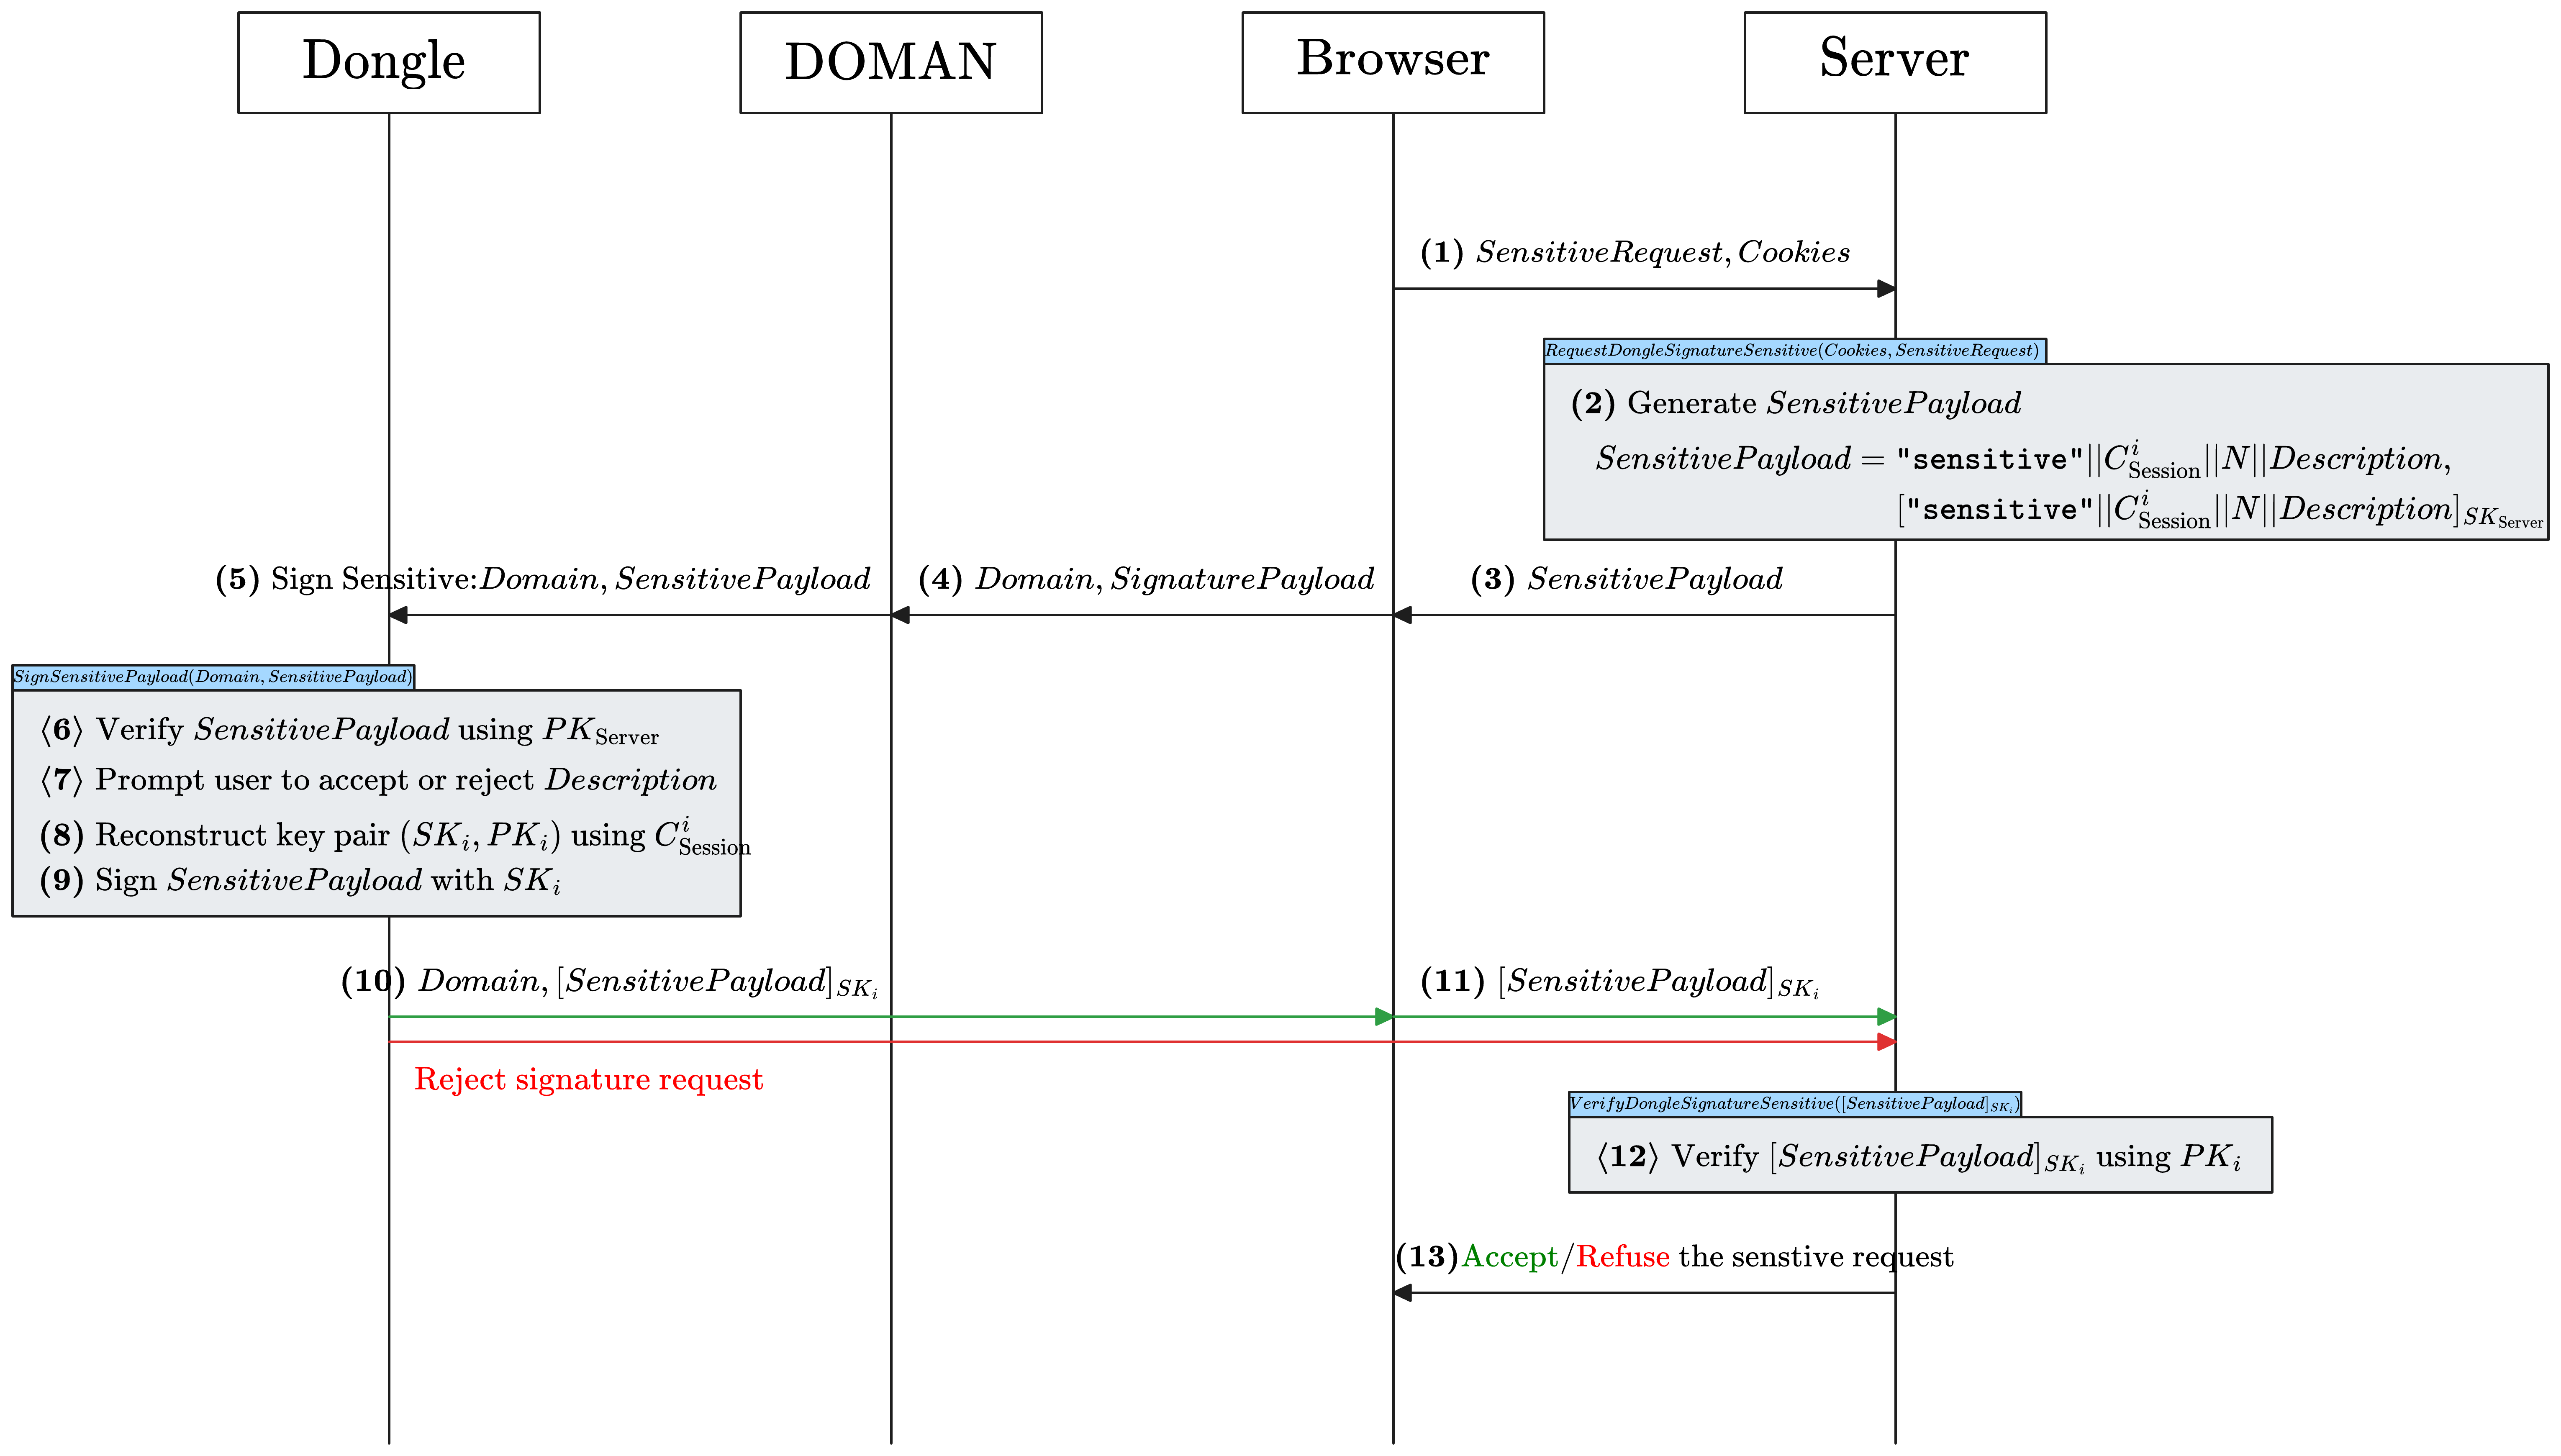
\includegraphics[width=1.25\linewidth]{img/REPUSH-2-Sensitive.png}
    \caption{Phase 2: Operation Phase - Sensitive Requests}
    \label{fig:REPUSH-phase-2-sensitive}
\end{figure}

The second mode of operation occurs in parallel with the previously presented continuous session authentication. It is used to handle sensitive requests. Again, what counts as "sensitive" is a judgment to be made by the server or application. For example, email change, making a post or a comment could be considered as "sensitive". During this phase (Figure \ref{fig:REPUSH-phase-2-sensitive}), the sensitive request must be verified and explicitly accepted by the user on the dongle's screen before it gets signed and sent to the server. This phase is composed of the following steps:

\paragraph{$\boldsymbol{(1)}$} The user through the browser makes some sensitive request to the server and presents the $Cookies$ along. When received, the server runs $RequestDongleSignatureSensitive(Cookies, SensitiveRequest)$ (Algorithm \ref{alg:request-dongle-signature-sensitive}).
\begin{algorithm}[ht!]
\caption{$RequestDongleSignatureSensitive(Cookies, SensitiveRequest)$}
\begin{algorithmic}[1]
    \Require Sensitive application request $SensitiveRequest$ with $Cookies$, and per-session state including $C^i_{\text{Session}}$.
    \Ensure  $SensitivePayload$ returned to the browser.
    \State $N \leftarrow TRNG()$
    \State $C^i_{\text{Session}} \leftarrow Fetch(Cookies)$
    \State $Description \leftarrow Describe(SensitiveRequest)$
    \State $\begin{aligned}[t]
        SensitivePayload \leftarrow (
        &\texttt{"sensitive"} || C^i_{\text{Session}} || N || Description,\\
        &[\texttt{"sensitive"} || C^i_{\text{Session}} || N || Description]_{SK_{\text{Server}}})
        \end{aligned}$
    \State \textbf{return} $SensitivePayload$
\end{algorithmic}
\label{alg:request-dongle-signature-sensitive}
\end{algorithm}
\paragraph{$\boldsymbol{(2)}$} $SensitivePayload$ is generated as: 
$$SensitivePayload= \texttt{"sensitive"} || C^i_{\text{Session}} || N || Description,
        [\texttt{"sensitive"} || C^i_{\text{Session}} || N || Description]_{SK_{\text{Server}}}$$
Where the challenge $C_\text{Session}^i$ is the one associated with the cookies, $N$ is a nonce and $Description$ is derived from the purpose of $SensitiveRequest$.
\paragraph{$\boldsymbol{(3)}$, $\boldsymbol{(4)}$ and $\boldsymbol{(5)}$} $SensitivePayload$ is sent to the browser. Then the browser sends $Domain$ and $SensitivePayload$ to DOMAN, which then forwards it to the dongle as a signature request to run the function $SignSensitivePayload(Domain, SensitivePayload)$ (Algorithm \ref{alg:sign-sensitive-payload}).
\begin{algorithm}[ht!]
\caption{$SignSensitivePayload(Domain, SensitivePayload)$}
\begin{algorithmic}[1]
    \Require $(Domain, SensitivePayload)$ received from the browser.
    \Ensure  $(Domain, [SensitivePayload]_{SK_i})$ returned to the browser, or an error.
    \State $V_{Payload} \leftarrow Verify(SensitivePayload, PK_{\text{Server}})$
    \If{$V_{Payload} = \text{failed}$}
        \State \textbf{return} "Reject signature request"
    \EndIf
    \State $\texttt{"sensitive"}, C^i_{\text{Session}}, N, Description \leftarrow SensitivePayload$
    \State $P \leftarrow UserConfirm(Description)$
    \If{$P = \text{reject}$}
        \State \textbf{return} "User rejected sensitive request"
    \EndIf
%    \State $seed'_i \leftarrow LR\text{-}PUF(S_0^{Domain},\ C^i_{\text{Session}})$
%    \State $seed_i \leftarrow ErrorCorrect(seed'_i)$
    \State $seed_i \leftarrow query_{BCH}(Domain, C^i_\text{Session})$
    \State $SK_i,\ PK_i \leftarrow KeyGen(seed_i)$
    \State $[SensitivePayload]_{SK_i} \leftarrow Sign(SensitivePayload, SK_i)$
    \State \textbf{return} $(Domain, [SensitivePayload]_{SK_i})$
\end{algorithmic}
\label{alg:sign-sensitive-payload}
\end{algorithm}
\paragraph{$\boldsymbol{\langle6\rangle}$} Verify the received $SensitivePayload$ using $PK_\text{Server}$ to make sure that the signature request is coming from the server.
\paragraph{$\boldsymbol{(7)}$} Prompt the user on the dongle's touch screen to accept the sensitive request by displaying $Description$, as seen in figure \ref{fig:sensitive-prompt-screen}.
\begin{figure}
    \centering
    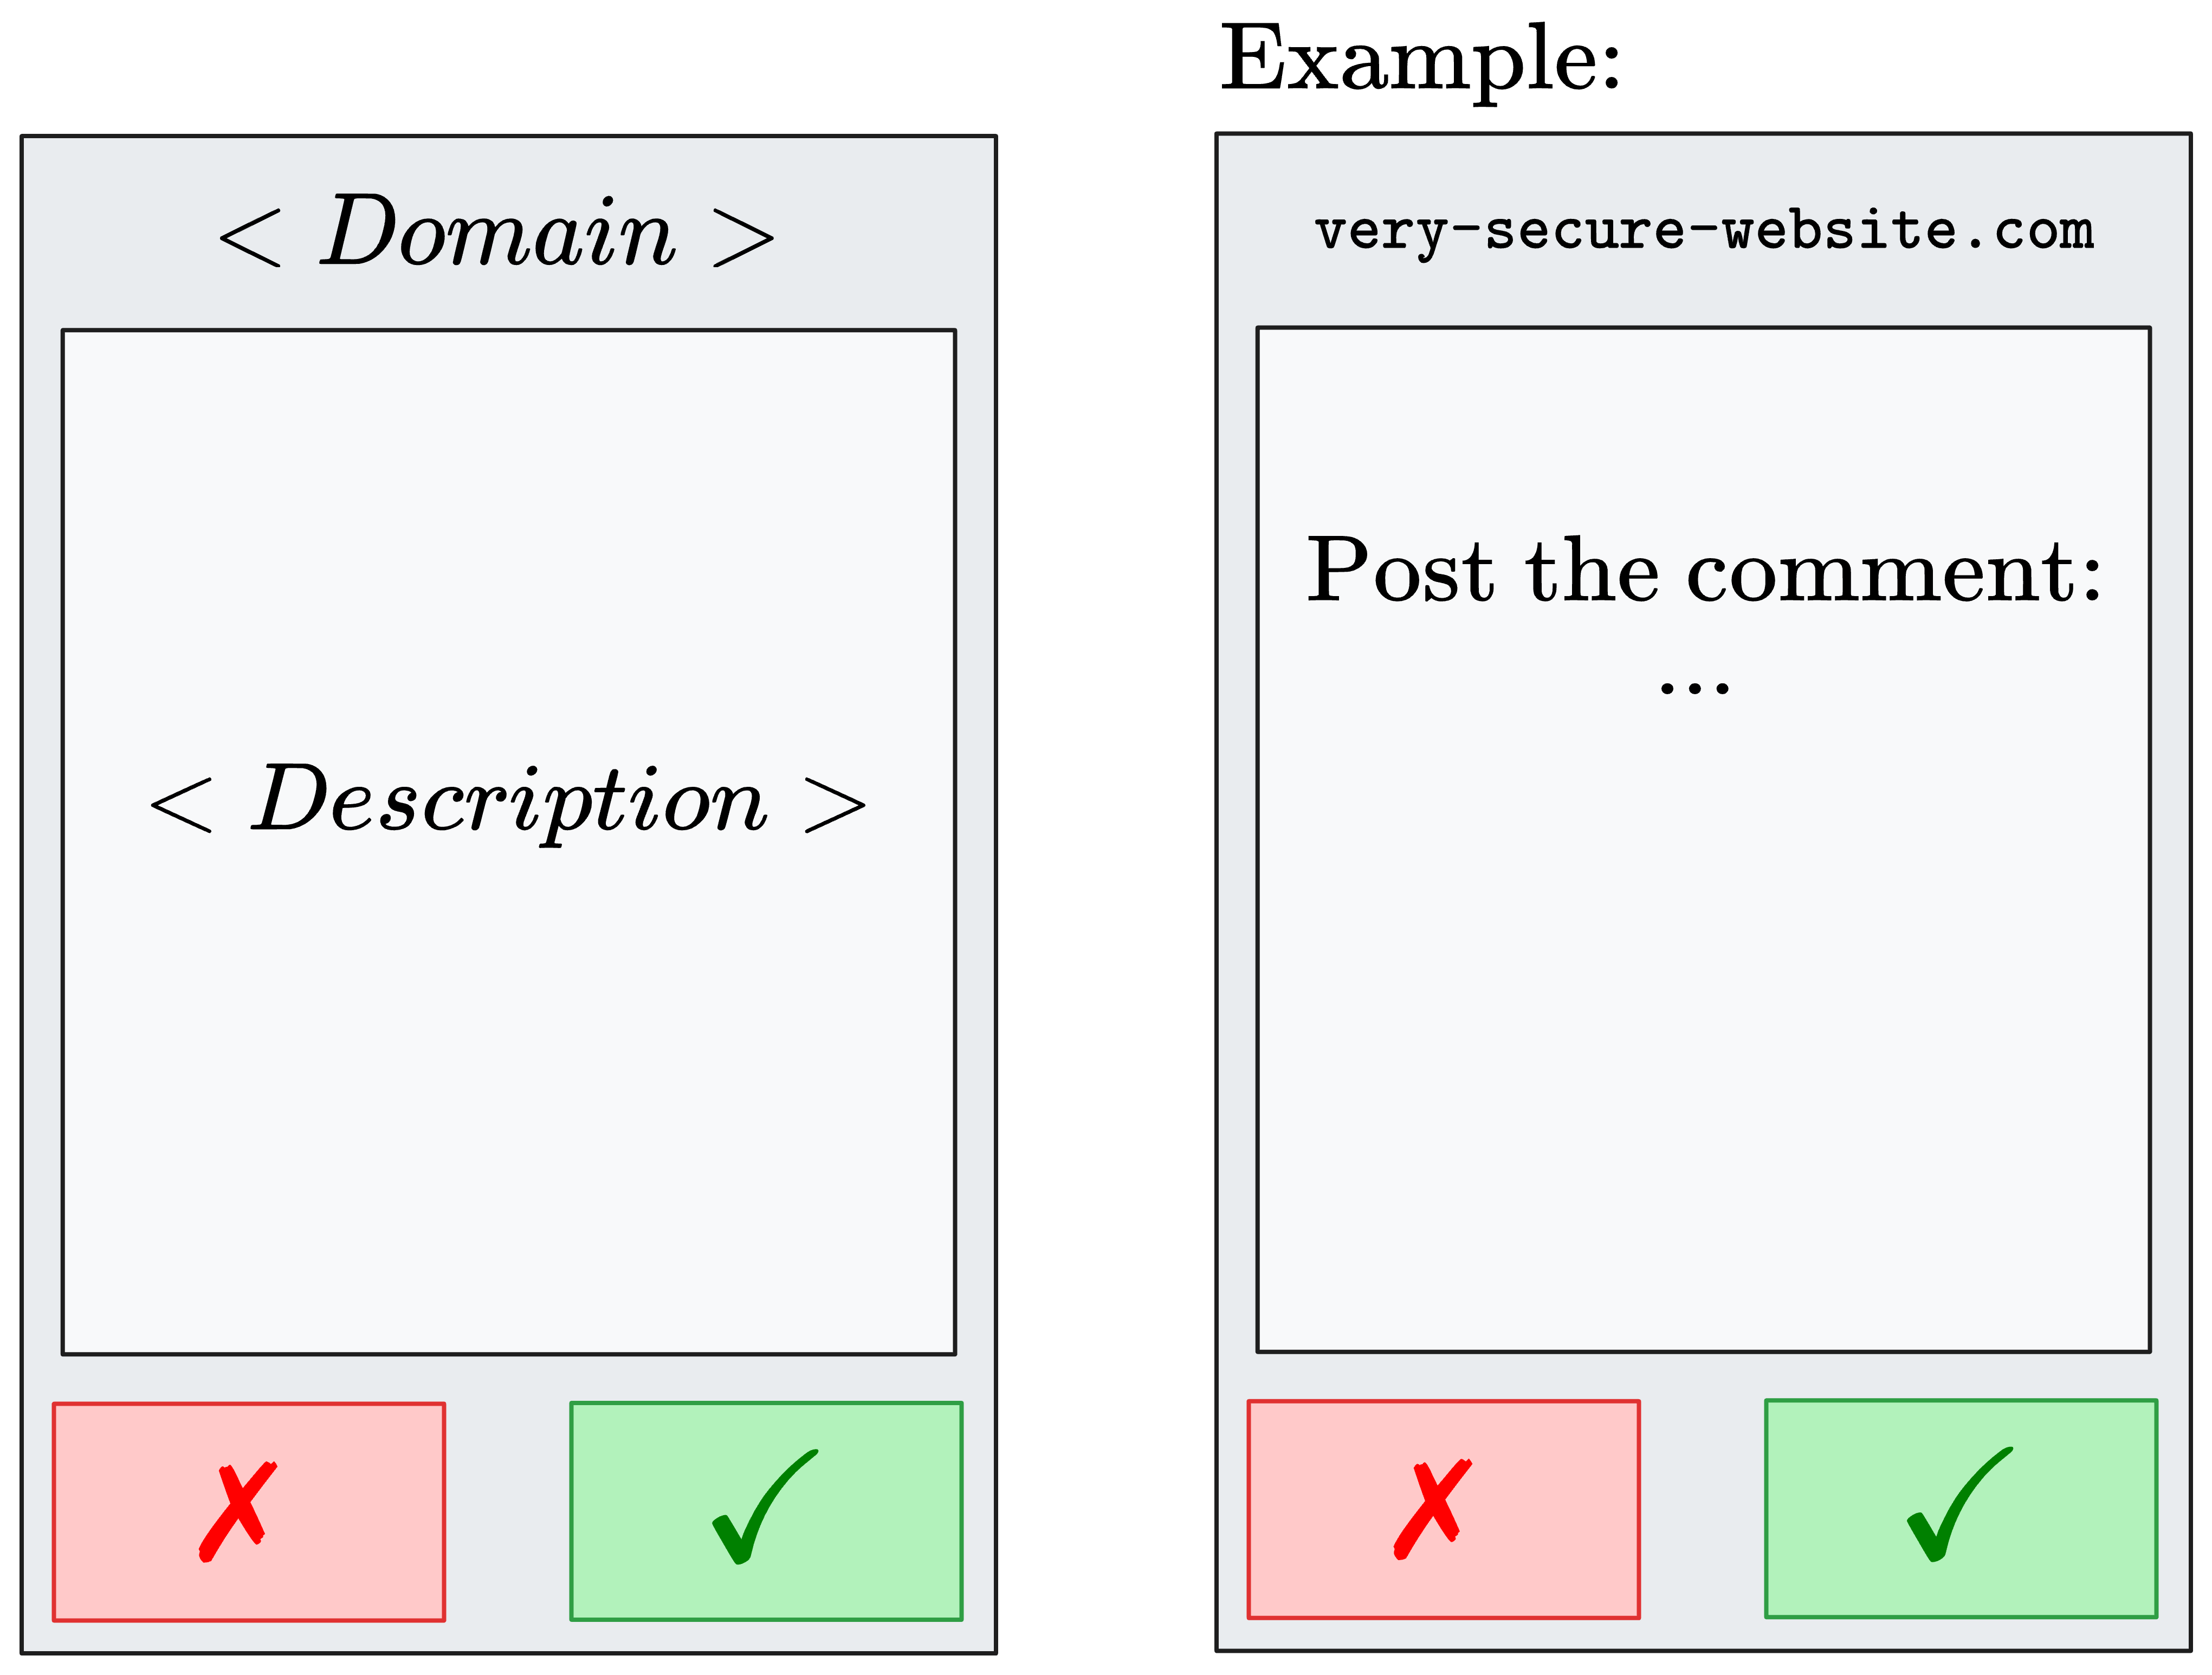
\includegraphics[width=0.5\linewidth]{img/touch-screen-accept-prompt.png}
    \caption{User prompt for accepting or refusing a sensitive request.}
    \label{fig:sensitive-prompt-screen}
\end{figure}
\paragraph{$\boldsymbol{(8)}$}If the user accepts the prompt, query the LR-PUF using the challenge $C_\text{Session}^i$ found within $SensitivePayload$ and the $Domain$ with $query_{BCH}$ to get as a response the error-corrected $seed_i$ before passing it to $KeyGen(seed_i)$ to generate the key pair $(SK_i,PK_i)$.
\paragraph{$\boldsymbol{(9)}$} Sign $SensitivePayload$ with $SK_i$ to prove to the server that the dongle possesses the private key $SK_i$ associated with the currently enrolled session public key $PK_i$.
\paragraph{$\boldsymbol{(10)}$ and $\boldsymbol{(11)}$} $Domain$ and $[SensitivePayload]_{SK_i}$ are sent to the browser. Then the browser sends $[SensitivePayload]_{SK_i}$ as a response to the server to prove ownership of the dongle and user approval of the request. When received, the server will run the function $VerifyDongleSignatureSensitive([SensitivePayload]_{SK_i})$ (Algorithm \ref{alg:verify-dongle-signature-sensitive}).
\begin{algorithm}[ht!]
\caption{$VerifyDongleSignatureSensitive([SensitivePayload]_{SK_i})$}
\begin{algorithmic}[1]
    \Require $[SensitivePayload]_{SK_i}$ and $Cookies$ received from the browser.
    \Ensure  The sensitive request is executed on a valid signature;
             otherwise it is refused.
    \State $V \leftarrow Verify([SensitivePayload]_{SK_i}, SensitivePayload, PK_i)$
    \If{$V = \text{failed}$}
        \State \textbf{return} "Refuse sensitive request"
    \EndIf
    \State $Execute(SensitiveRequest)$
    \State \textbf{return} "Accept sensitive request"
\end{algorithmic}
\label{alg:verify-dongle-signature-sensitive}
\end{algorithm}
\paragraph{$\boldsymbol{\langle12\rangle}$} The server verifies $[SensitivePayload]_{SK_i}$ using $PK_i$.
\paragraph{$\boldsymbol{(13)}$} If the signature is valid, the sensitive request is executed, otherwise, it is refused.

\subsection{Phase 3: Reconfiguration Phase}
The third phase of the protocol described in figure \ref{fig:REPUSH-phase-3} exploits the reconfigurability of the LR-PUF to generate a new key for extending a session. After some time $T_\text{Expiry}$, the session expires and a new key is required in case the user wants to extend the session. Here the following time variables are taken into consideration:
\begin{itemize}
    \item $T_\text{Expiry}$: The maximum session time after which the server requests a session extension by key rotation. Typically $T_\text{Expiry} \gg T_\text{Validity}$. 
    \item $t_\text{start}^{Session}$: Timestamp of when the current session started.
\end{itemize}

\begin{figure}
    \centering
    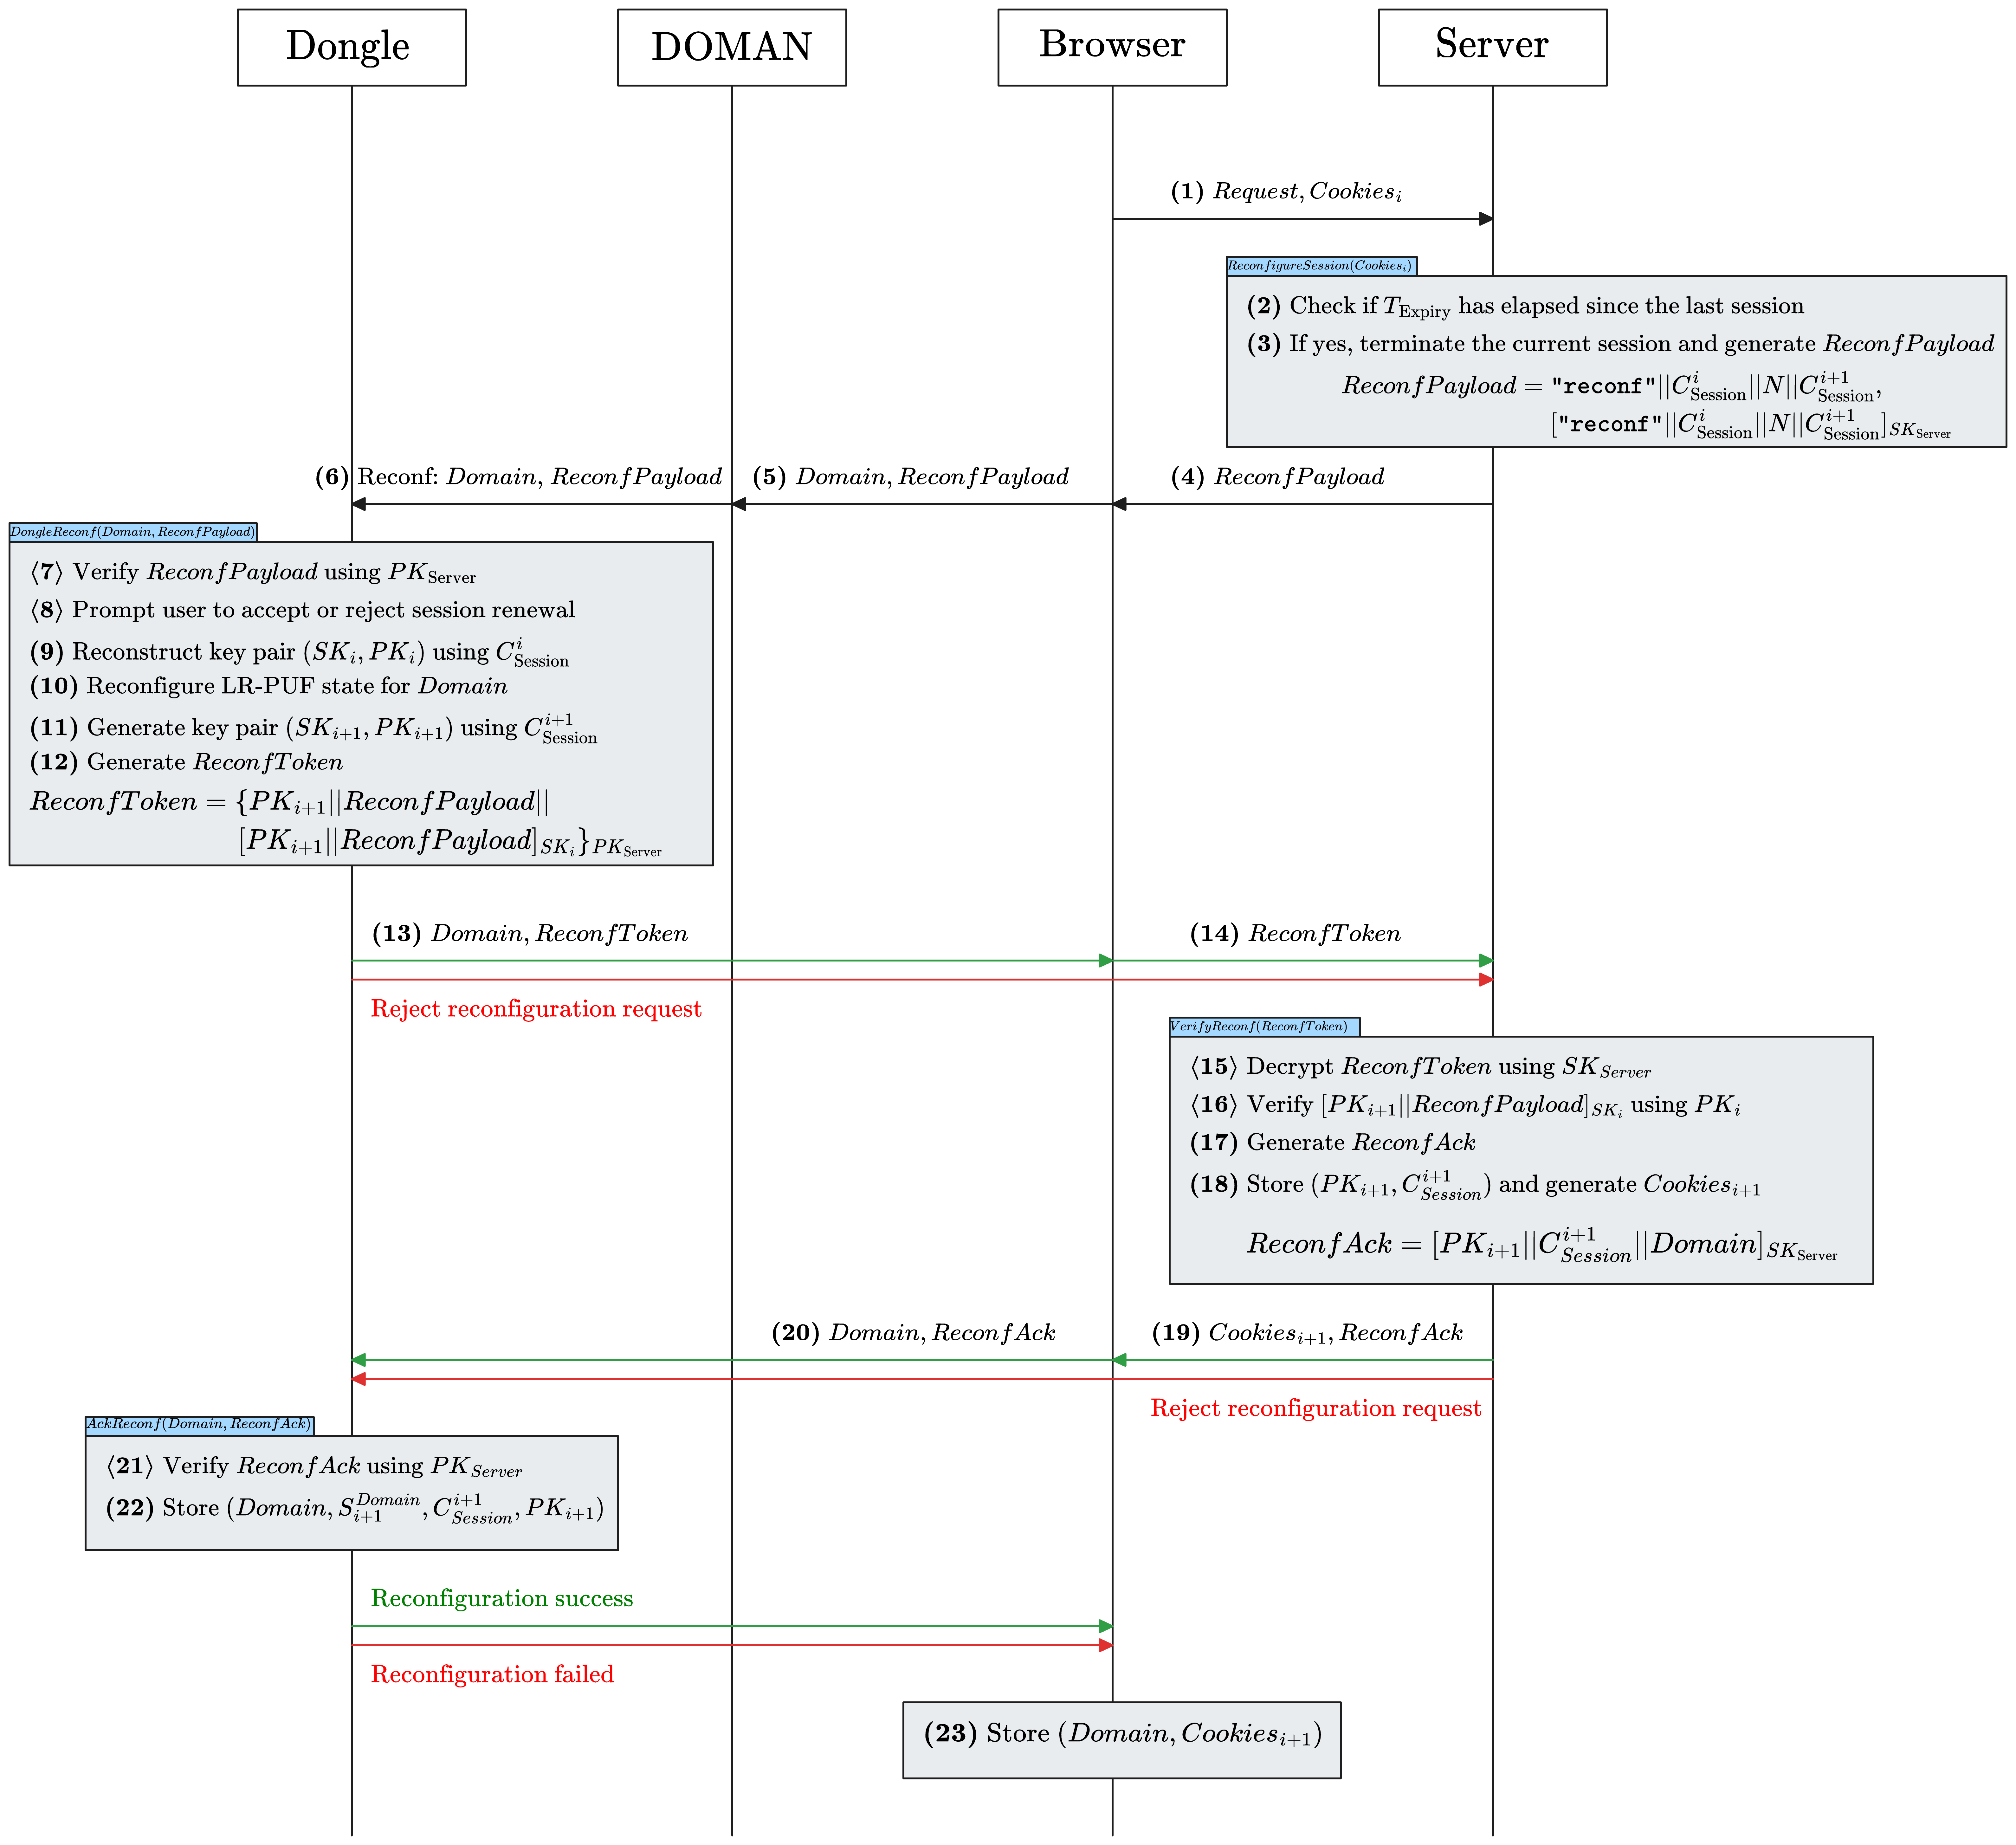
\includegraphics[width=1.2\linewidth]{img/REPUSH-3.png}
    \caption{Phase 3: Reconfiguration Phase}
    \label{fig:REPUSH-phase-3}
\end{figure}

This phase of the protocol is composed of the following steps:
\paragraph{$\boldsymbol{(1)}$} The user makes any request from the browser to the server and presents the current $Cookies_i$. On every received request, the server runs the function $ReconfigureSession(Cookies_i)$ (Algorithm \ref{alg:reconfigure-session}).
\begin{algorithm}[ht!]
\caption{$ReconfigureSession(Cookies_i)$}
\begin{algorithmic}[1]
    \Require Incoming request with $Cookies_i$;
             per-session state including $t^{Session}_{\text{start}}$, $C^i_{\text{Session}}$, and $PK_i$.
    \Ensure  $ReconfPayload$ returned to the browser when the session has expired, otherwise the request is served normally.
    \State $\Delta_\text{Elapsed} \leftarrow Now() - t^{Session}_{\text{start}}$
    \If{$\Delta_\text{Elapsed} < T_{\text{Expiry}}$}
        \State \textbf{return} \texttt{NULL} \Comment{session still within its lifetime}
    \EndIf
    \State $C^i_{\text{Session}} \leftarrow Fetch(Cookies_i)$
    \State $Terminate(Cookies_i)$ \Comment{stop serving requests under the old session}
    \State $N \leftarrow TRNG()$
    \State $C^{i+1}_{\text{Session}} \leftarrow TRNG()$
    \State $m \leftarrow \texttt{"reconf"} || C^i_{\text{Session}} || N || C^{i+1}_{\text{Session}}$
    \State $ReconfPayload \leftarrow (m, [m]_{SK_{\text{Server}}})$
    \State \textbf{return} $ReconfPayload$
\end{algorithmic}
\label{alg:reconfigure-session}
\end{algorithm}
\paragraph{$\boldsymbol{(2)}$} The server checks if $T_\text{Expiry}$ has elapsed since the start of the session to determine if the session has expired or not.
\paragraph{$\boldsymbol{(3)}$} If $T_\text{Expiry}$ has elapsed, then the current session is terminated and we generate $ReconfPayload$ to ask the dongle for a new key:
$$ReconfPayload = (\texttt{"reconf"} || C^i_{\text{Session}} || N || C^{i+1}_{\text{Session}}, [\texttt{"reconf"} || C^i_{\text{Session}} || N || C^{i+1}_{\text{Session}}]_{SK_\text{Server}})$$
\paragraph{$\boldsymbol{(4)}$, $\boldsymbol{(5)}$ and $\boldsymbol{(6)}$} $ReconfPayload$ is sent to the browser. Then the browser sends $Domain$ and $ReconfPayload$ to DOMAN, which then forwards it to the dongle as a reconfiguration request to run the function $DongleReconf(Domain, ReconfPayload)$.
\begin{algorithm}[ht!]
\caption{$DongleReconf(Domain, ReconfPayload)$}
\begin{algorithmic}[1]
    \Require $(Domain, ReconfPayload)$ received from the browser.
    \Ensure  $(Domain, ReconfToken)$ returned to the browser, or an error.
    \State $V_{Payload} \leftarrow Verify(ReconfPayload, PK_{\text{Server}})$
    \If{$V_{Payload} = \text{failed}$}
        \State \textbf{return} "Reject reconfiguration request"
    \EndIf
    \State $\texttt{"reconf"}, C^i_{\text{Session}}, N, C^{i+1}_{\text{Session}} \leftarrow ReconfPayload$
    \State $P \leftarrow UserConfirm(Domain)$
    \If{$P = \text{reject}$}
        \State \textbf{return} "User rejected session renewal"
    \EndIf
%    \State $seed'_i \leftarrow query(C^i_{\text{Session}},Domain)$
%    \State $seed_i \leftarrow ErrorCorrect(seed'_i)$
    \State $seed_i \leftarrow query_{BCH}(Domain, C_\text{Session}^i)$
    \State $SK_i,\ PK_i \leftarrow KeyGen(seed_i)$
%    \State $reconfigure(Domain)$ \Comment{Sets $S^{Domain}_{i+1}$}
%    \State $seed_{i+1} \leftarrow query(C^{i+1}_{\text{Session}},Domain)$
    \State $seed_{i+1} \leftarrow enroll_{BCH}(Domain, C^{i+1}_{\text{Session}},10)$
    \State $SK_{i+1},\ PK_{i+1} \leftarrow KeyGen(seed_{i+1})$
    \State $ReconfToken \leftarrow \{PK_{i+1} || ReconfPayload || [PK_{i+1} || ReconfPayload]_{SK_i}\}_{PK_{\text{Server}}}$
    \State \textbf{return} $(Domain,\ ReconfToken)$
\end{algorithmic}
\label{alg:dongle-reconf}
\end{algorithm}
\paragraph{$\boldsymbol{\langle7\rangle}$} Verify the received $ReconfPayload$ using $PK_\text{Server}$ to make sure that the reconfiguration request is coming from the server.
\paragraph{$\boldsymbol{\langle8\rangle}$} Prompt the user to accept or reject the session renewal or configuration (Figure \ref{fig:sension-renewal-prompt-screen}).
\begin{figure}
    \centering
    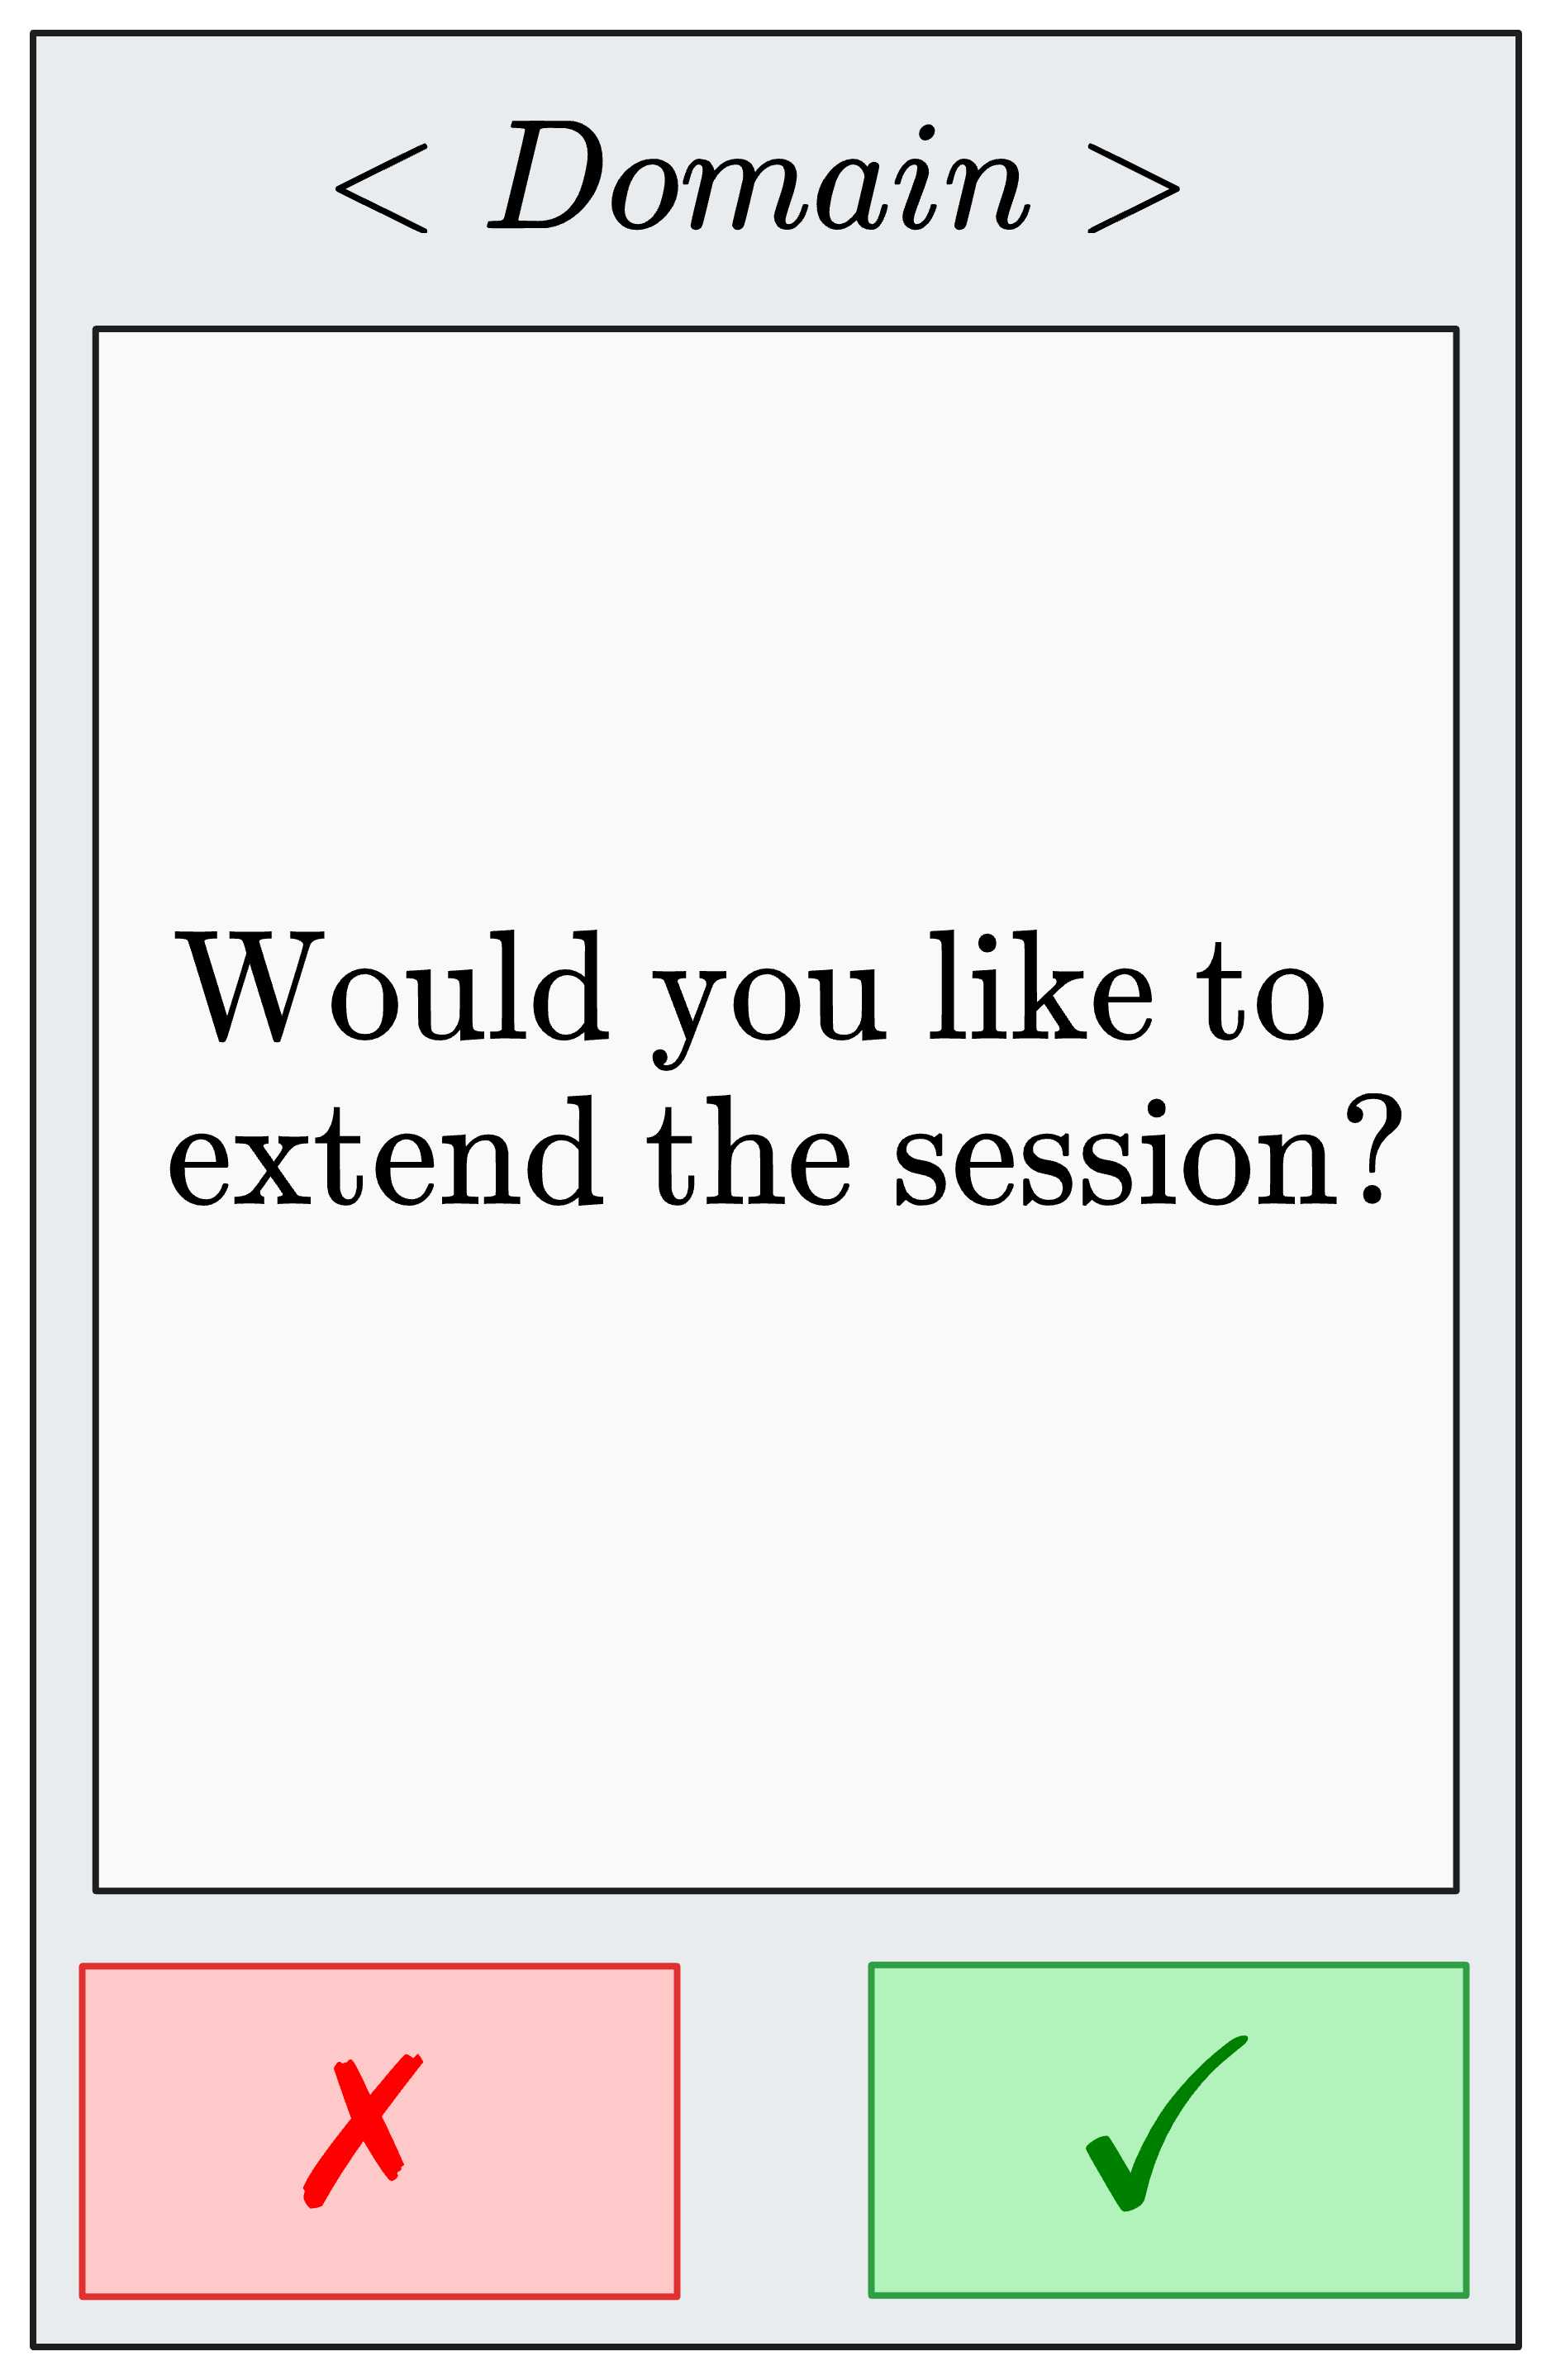
\includegraphics[width=0.3\linewidth]{img/user-prompt-session-renewalp.png}
    \caption{User prompt for session renewal.}
    \label{fig:sension-renewal-prompt-screen}
\end{figure}

\paragraph{$\boldsymbol{(9)}$} If the user accepts the prompt, query the LR-PUF with the $query_{BCH}$ function using the current challenge $C_\text{Session}^i$ found within $ReconfPayload$ and $Domain$ to get the error-corrected $seed_i$ as a response. Then $KeyGen(seed_i)$ is used to generate the key pair $(SK_i,PK_i)$.

\paragraph{$\boldsymbol{(10)}$ and $\boldsymbol{(11)}$} Generate a new key pair for the new session by running $enroll_{BCH}(Domain, C_\text{Session}^{i+1}, 10)$, which will actually run $reconfigure(Domain)$ to get a new state $S_{i+1}^{Domain}$ and then use the new challenge to enroll a new $seed_{i+1}$ which can be error-corrected and then use it to generate the new key pair $(SK_{i+1}, PK_{i+1})$.
\paragraph{$\boldsymbol{(12)}$} $ReconfToken$ is generated as follows to prove to the server that the dongle possesses the current session private key $SK_i$ and then use that to transfer the trust to the new public key $PK_{i+1}$, and the whole token is encrypted with $PK_\text{Server}$ so that only the server can decrypt its contents:
$$ReconfToken = \{PK_{i+1} || ReconfPayload || [PK_{i+1} || ReconfPayload]_{SK_i}\}_{PK_{\text{Server}}}$$
\paragraph{$\boldsymbol{(13)}$ and $\boldsymbol{(14)}$} $Domain$ and $ReconfToken$ are sent to the browser. Then the browser sends $ReconfToken$ as a response to the server. When received, the server runs the function $VerifyReconf(ReconfToken)$ (Algorithm \ref{alg:verify-reconf}).

\begin{algorithm}[ht!]
\caption{$VerifyReconf(ReconfToken)$}
\begin{algorithmic}[1]
    \Require $ReconfToken$ received from the browser.
    \Ensure  $(Cookies_{i+1}, ReconfAck)$ returned to the browser, or an error.
    \State $D \leftarrow Decrypt(ReconfToken, SK_{\text{Server}})$
    \If{$D = \text{failed}$}
        \State \textbf{return} ``Reject reconfiguration request''
    \EndIf
    \State $PK_{i+1},ReconfPayload,[PK_{i+1}||ReconfPayload]_{SK_i} \leftarrow D$
    \State $V \leftarrow Verify([PK_{i+1}||ReconfPayload]_{SK_i}, PK_{i+1}||ReconfPayload, PK_i)$
    \If{$V = \text{failed}$}
        \State \textbf{return} ``Reject reconfiguration request''
    \EndIf
    \State $\texttt{"reconf"}, C^i_{\text{Session}}, N, C^{i+1}_{\text{Session}} \leftarrow ReconfPayload$
    \State $ReconfAck \leftarrow [PK_{i+1}|| C^{i+1}_{\text{Session}}|| Domain]_{SK_{\text{Server}}}$
    \State $store(PK_{i+1},\ C^{i+1}_{\text{Session}})$
    \State $Cookies_{i+1} \leftarrow GenerateCookies()$
    \State $t^{Session}_{\text{last}} \leftarrow Now()$ 
    \State $t^{Session}_{\text{start}} \leftarrow Now()$
    \State \textbf{return} $(Cookies_{i+1}, ReconfAck)$
\end{algorithmic}
\label{alg:verify-reconf}
\end{algorithm}
\paragraph{$\boldsymbol{\langle15\rangle}$} The server decrypts $ReconfToken$ using $SK_\text{Server}$ to get $PK_{i+1}$.
\paragraph{$\boldsymbol{\langle16\rangle}$} $[PK_{i+1}||ReconfPayload]_{SK_i}$ is verified using $PK_i$ to establish that the dongle did produce ${PK_{i+1}}$ and received $ReconfPayload$.
\paragraph{$\boldsymbol{(17)}$} A reconfiguration acknowledgment $ReconfAck$ is generated as follows to prove to the dongle that the server did receive the $ReconfToken$:
$$ReconfAck=[PK_{i+1}|| C^{i+1}_{\text{Session}}|| Domain]_{SK_{\text{Server}}}$$
\paragraph{$\boldsymbol{(18)}$} A new session is created by associating $PK_{i+1}$ with $C^{i+1}_{Session}$ and generating new $Cookies_{i+1}$.
\paragraph{$\boldsymbol{(19)}$} $Cookies_{i+1}$ and $ReconfAck$ are sent to the browser.
\paragraph{$\boldsymbol{(20)}$} $Cookies_{i+1}$ stay in the browser, and $ReconfAck$ and $Domain$ are sent to the dongle for it to run $AckReconf(Domain, ReconfAck)$ (Algorithm \ref{alg:ack-reconf}).
\begin{algorithm}[ht!]
\caption{$AckReconf(Domain, ReconfAck)$}
\begin{algorithmic}[1]
    \Require $(Domain, ReconfAck)$ received from the browser.
    \Ensure  Reconfiguration success and persisted state
             $(Domain, S^{Domain}_{i+1}, C^{i+1}_{\text{Session}}, PK_{i+1})$.
             Otherwise, a reconfiguration error is returned.
    \State $V_{ReconfAck} \leftarrow
            Verify(ReconfAck, PK_{i+1} || C^{i+1}_{\text{Session}} || Domain, PK_{\text{Server}})$
    \If{$V_{ReconfAck} = \text{failed}$}
        \State \textbf{return} ``Reconfiguration not acknowledged''
    \EndIf
    \State $store(Domain, S^{Domain}_{i+1}, C^{i+1}_{\text{Session}},\ PK_{i+1})$
    \State \textbf{return} ``Reconfiguration success''
\end{algorithmic}
\label{alg:ack-reconf}
\end{algorithm}
\paragraph{$\boldsymbol{\langle21\rangle}$} The signature $ReconfAck$ is verified using $PK_{Server}$. If this step fails a reconfiguration error is returned to the browser.
\paragraph{$\boldsymbol{(22)}$} The tuple $(Domain, S_{i+1}^{Domain}, C_{Session}^{i+1}, PK_{i+1})$ is stored on the dongle for it to be used from now on to verify dongle ownership and sign sensitive requests.
\paragraph{$\boldsymbol{(23)}$} On reconfiguration success, $(Domain, Cookies_{i+1})$ is stored on the browser.

By the end of the reconfiguration phase, $PK_{i+1}$ will now be used to verify any signature coming from the dongle. The trust is transferred from $PK_i$ to $PK_{i+1}$. After this the protocol goes back to the second phase until $T_{Expiry}$ is elapsed and a reconfiguration is in order.

% !TeX encoding = UTF-8
% !TeX spellcheck = en_GB
% !TeX root = ../thesis.tex

\chapter{Implementation}
\label{chapter:implementation}
This chapter describes the practical implementation of the REPUSH protocol. Each of the sections below describes the design decisions and non-obvious engineering choices that emerged during development. The following public repositories contain the source code and instructions on how to set up everything. To reproduce, the reader should start with the \verb|README| file on the Arduino implementation repository:
\begin{itemize}
    \item Dongle:
    \begin{itemize}
    \item Arduino: \url{https://github.com/ilyasben26/REPUSH-Dongle}
     \item FPGA: \url{https://github.com/ilyasben26/REPUSH-FPGA}
    \end{itemize}
    \item DOMAN: \url{https://github.com/ilyasben26/REPUSH-DOMAN}
    \item Server: \url{https://github.com/ilyasben26/REPUSH-Server}
\end{itemize}



\subsubsection{Notice}
During the implementation of the REPUSH protocol, the coding assistant tools Claude Code \cite{claude_code_docs} and GitHub Copilot \cite{github_copilot} were used to assist with development. All generated code and recommendations were reviewed and validated.



\section{System Architecture}
Figure \ref{fig:physical-implementation} shows the real components of the implemented REPUSH protocol and the communication channels between them.

\begin{figure}
    \centering
    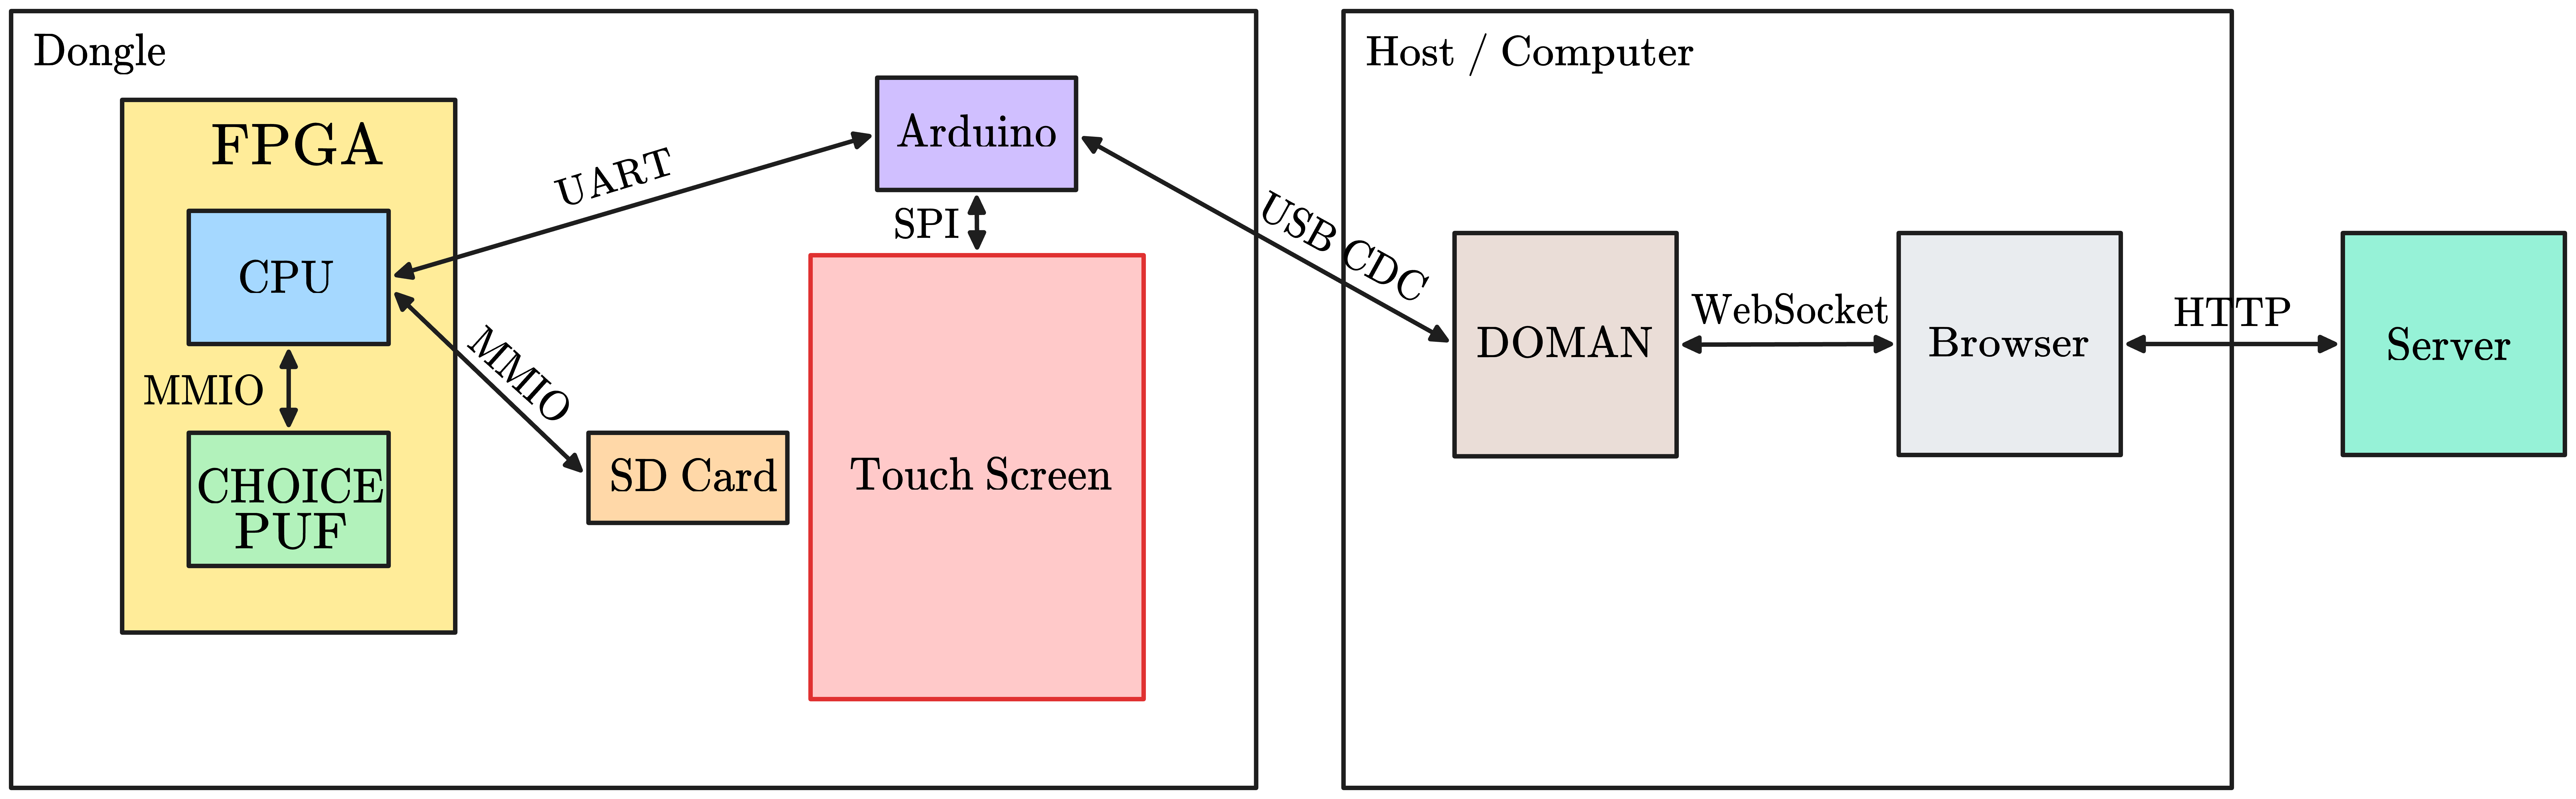
\includegraphics[width=\linewidth]{img/system-implementation.png}
    \caption{Physical implementation components}
    \label{fig:physical-implementation}
\end{figure}

The FPGA and the Arduino communicate over UART using a custom binary framing protocol that will be explained later. The FPGA implements the CPU and the CHOICE PUF, both of which are defined using Verilog and VHDL respectively. The CHOICE PUF and the SD card are exposed as peripherals to the CPU and communication is done via MMIO (Memory-Mapped I/O). The FPGA-defined CPU is used to augment the CHOICE PUF to an LR-PUF by carrying out the necessary hashing and storing of the states on the SD card. The Arduino board communicates with the touch screen via SPI (Serial Peripheral Interface). The Arduino communicates with the computer via DOMAN over a USB CDC (Universal Serial Bus Communications Device Class) serial port. DOMAN is a local server that exposes a WebSocket endpoint that the Javascript on the browser uses to talk to the dongle. The browser communicates with the server via HTTP since actually the server in this implementation is running locally on the host for test purposes.
\section{Dongle Implementation}
A picture of the actual dongle can be seen in figure \ref{fig:real-dongle}. The two buttons next to the touch screen are optional and could be used later for accepting or refusing the sensitive requests.

\begin{figure}
    \centering
    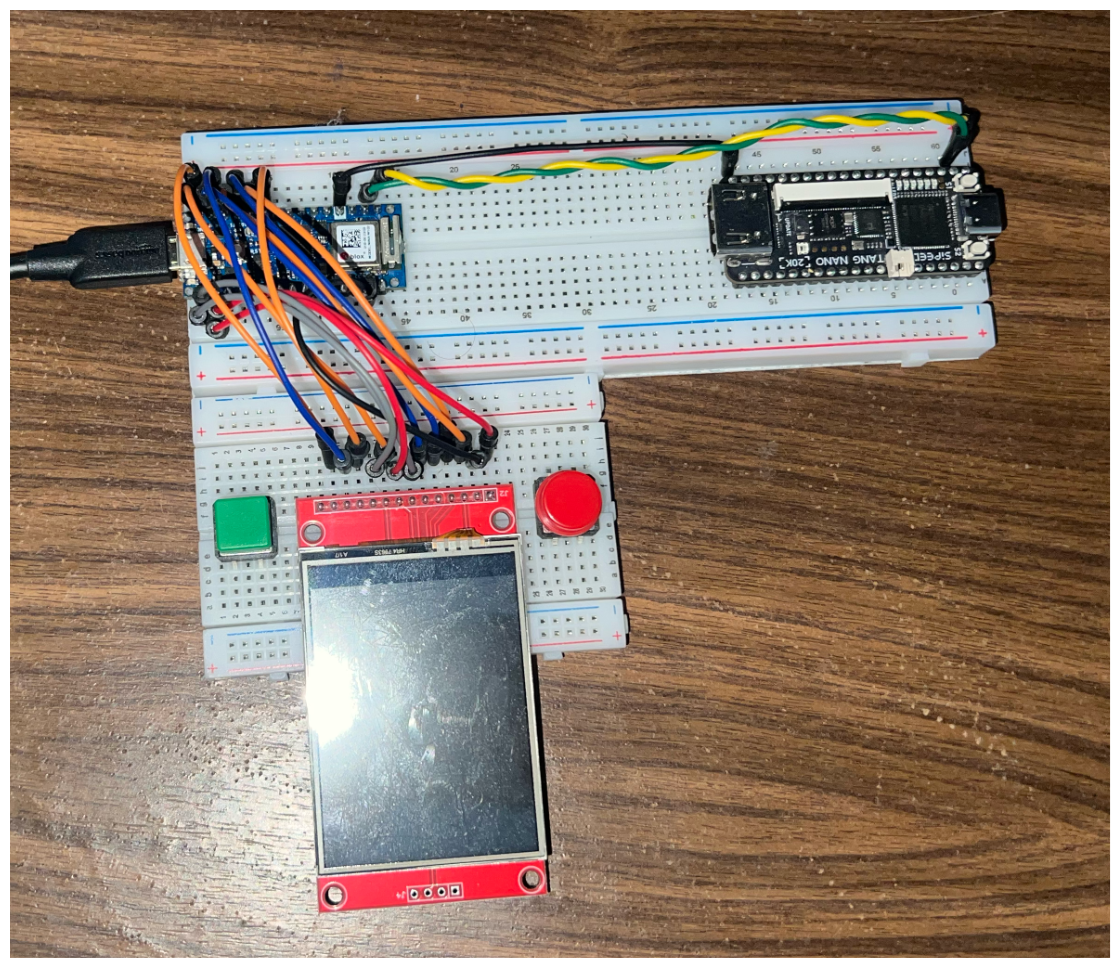
\includegraphics[width=0.6\linewidth]{img/real-dongle.png}
    \caption{Picture of the dongle}
    \label{fig:real-dongle}
\end{figure}

The FPGA part of the dongle handles the LR-PUF logic, whilst the Arduino handles communication with the host computer, cryptographic operations and drives the touch screen display. The raw CHOICE-PUF responses never exit the fabric of the FPGA, rather the Arduino has a list of commands it can issue to the FPGA to only carry out the necessary LR-PUF logic.


\subsection{FPGA Implementation}
The code for the FPGA implementation including the firmware can be found in the repository titled \verb|REPUSH-FPGA|, the \verb|README| file of the repository describes the project structure and how to compile, synthesize and flash the FPGA with the implementation.

The used FPGA board is a Sipeed Tang Nano 20k development board \cite{sipeed_tang_nano_20k} which hosts a Gowin GW2AR-18 FPGA chip. The implemented CPU is a PicoRV32 RISC-V core \cite{picoRV32} defined in Verilog. The CPU implementation and the firmware for it was originally taken from \cite{picorv32_tang_nano_unified} and expanded to accommodate the CHOICE-PUF as a peripheral and carry out all the necessary LR-PUF operations. The CHOICE-PUF VHDL implementation was taken from the Github repository \cite{choice_puf_repo} mentioned in the CHOICE-PUF paper \cite{9556423} and was modified to work on the targeted GW2AR-18 FPGA chip since the original implementation was meant for a Xilinx FPGA, a controller state-machine was added to control the CHOICE-PUF via MMIO from the CPU.

\subsubsection{PicoRV32 Core Configuration}
The PicoRV32 core is instantiated with the parameters listed in table \ref{tab:picorv32-params}. The CPU runs at a frequency of 9 MHz which is obtained from the 27 MHz oscillator of the board using the on-chip rPLL (rational Phase-Locked Loop). The CPU has access to 64 KB of SRAM defined using $\verb|SRAM_ADDR_WIDTH|=14$, which gives $2^{14}=65\,536~bytes$. Since the SRAM serves as both instruction memory and data memory within a fixed-size region, there is no heap and would-be dynamic allocations are replaced with static global variables. The compiled firmware occupies around 61 KB of the 64 KB SRAM. It is loaded at address \verb|PROGADDR_RESET = 0x00000000| and that is where the CPU begins executing the instructions at boot and on reset. Multiplication and division instructions were enabled since the firmware needs them for array indexing among other things. The stack starts at the top of the SRAM at address \verb|STACKADDR = 0x00010000| and grows downward, leaving only 3.2 KB of headroom for the stack. In practice, this small size proved to be sufficient. The barrel shifter and compressed ISA (Instruction Set Architecture) are disabled to reduce the footprint of the CPU on the FPGA. 

\begin{table}[ht!]
\centering
\caption{PicoRV32 parameters.}
\begin{tabular}{lll}
\hline
\textbf{Parameter} & \textbf{Value} & \textbf{Description} \\
\hline
Clock frequency     & 9~MHz          & Derived from 27~MHz crystal via rPLL \\
\texttt{SRAM\_ADDR\_WIDTH} & 14      & 64~KB combined instruction/data memory \\
\texttt{ENABLE\_MUL}       & 1       & Hardware 32$\times$32 multiplier \\
\texttt{ENABLE\_DIV}       & 1       & Hardware divider \\
\texttt{BARREL\_SHIFTER}   & 0       & Disabled; reduces LUT count \\
\texttt{COMPRESSED\_ISA}& 0       & 32-bit instructions (no RV32C compression) \\
\texttt{PROGADDR\_RESET}   & \texttt{0x00000000} & Boot vector (bottom of SRAM) \\
\texttt{STACKADDR}         & \texttt{0x00010000} & Initial stack pointer (top of SRAM) \\
\hline
\end{tabular}
\label{tab:picorv32-params}
\end{table}

\subsubsection{Memory-Mapped I/O}
As mentioned before, the CPU uses MMIO to interact with the CHOICE PUF and other peripherals. As seen in table \ref{tab:mmio-map}, each peripheral is assigned a fixed address range. When the CPU wants to use a peripheral, it puts its address on the bus \verb|mem_addr|, the data to write on \verb|mem_wdata|, and raises the \verb|mem_valid| signal. Once the \verb|mem_valid| signal is raised, every peripheral compares the value inside \verb|mem_addr| with its address range and the one whose range matches it raises its select signal. If it is a write transaction, the peripheral reads the data from \verb|mem_wdata| and acts on it. If it is a read transaction, the peripheral places its response on \verb|mem_rdata| for the CPU to read back. Once the peripheral has finished its task, it raises its ready signal which feeds into \verb|mem_ready|. The CPU stalls until \verb|mem_ready| goes high. 

\begin{table}[ht!]
\centering
\caption{MMIO address map.}
\begin{tabular}{lll}
\hline
\textbf{Address range} & \textbf{Peripheral} & \textbf{Description} \\
\hline
\texttt{0x00000000}--\texttt{0x0000FFFF} & SRAM            & 64~KB program and data memory \\
\texttt{0x80000000}                      & LEDs            & 6-bit on-board LED register \\
\texttt{0x80000008}--\texttt{0x8000000F} & Debug UART      & Serial console (TX/RX) \\
\texttt{0x80000010}                      & Countdown timer & Hardware timeout counter \\
\texttt{0x80000020}                      & WS2812b         & Addressable RGB LED driver \\
\texttt{0x80000030}--\texttt{0x8000003F} & SD SPI helper   & Byte-level SPI controller for SD card \\
\texttt{0x80000040}--\texttt{0x8000004F} & CHOICE-PUF      & PUF command/response registers \\
\texttt{0x80000058}--\texttt{0x8000005F} & Arduino UART    & UART to the Arduino board (TX/RX) \\
\hline
\end{tabular}
\label{tab:mmio-map}
\end{table}

The CHOICE PUF peripheral at base address \verb|0x80000040| exposes three 32-bit registers (Table \ref{tab:puf-regs}). Since the PicoRV32 is a 32-bit CPU and can only transfer 32 bits per transaction, the 64-bit command and response are each split across two buses that share the same addresses. Commands are written to \verb|payload_hi| and \verb|payload_lo|, where the top four bits of \verb|payload_hi| determine the command type (request measurement, set choice, set address tuning or load a pattern) and the parameters are passed in \verb|payload_lo|. Writing to the trigger register at \verb|0x80000048| executes the command defined within the buses. For reading the PUF's response, the firmware polls the status register at the same address \verb|0x80000048| until its bit[0] is set to 1 by the PUF to indicate that the 64-bit response of the PUF is accessible on \verb|0x80000040| and \verb|0x80000044| via the two buses \verb|response_hi| and \verb|response_lo|.


\begin{table}[ht!]
  \centering
  \caption{CHOICE-PUF peripheral address map.}
  \begin{tabular}{llll}
  \hline
  \textbf{Offset} & \textbf{Address} & \textbf{Write} & \textbf{Read} \\
  \hline
  \texttt{0x0} & \texttt{0x80000040} & \texttt{payload\_hi}: command bits [63:32]       & \texttt{response\_hi}: response [63:32] \\
  \texttt{0x4} & \texttt{0x80000044} & \texttt{payload\_lo}: command bits [31:0]         & \texttt{response\_lo}: response [31:0] \\
  \texttt{0x8} & \texttt{0x80000048} & \texttt{trigger}: a write executes the command    & \texttt{status}: bit[0]=1 if response ready \\
  \hline
  \end{tabular}
  \label{tab:puf-regs}
  \end{table}

\subsubsection{CHOICE-PUF Implementation}
The CHOICE-PUF VHDL implementation was taken from \cite{choice_puf_repo} and adapted to run on the GW2AR-18. In the original code, each PUF cell used 32-bit ASRs, which gave it a challenge space of $\binom{4}{2} \cdot 32^2 = 6144$ challenges. To reduce the footprint of the PUF on the FPGA, the ASRs were reduced to 8 bits, which reduced the challenge space to $\binom{4}{2} \cdot 8^2 = 384$ challenges. The PUF response width was also reduced from 128 bits to 64 bits to make it fit in the GW2AR-18.

The original CHOICE-PUF VHDL implementation was designed for a Xilinx Spartan-3E FPGA and relied on Xilinx-specific features that needed to be replaced with their Gowin counterparts:
\begin{itemize}
    \item \textbf{Shift register LUT primitives (\texttt{SRLC32E})}: The original ASRs were implemented using Xilinx \texttt{SRLC32E} primitives. Since no equivalent primitive exists on the GW2AR-18, they were replaced with 8-bit ASRs described behaviorally in VHDL.
    \item \textbf{Carry chain primitives (\texttt{CARRY4})}: The original implementation used the Xilinx \texttt{CARRY4} primitive to chain the four ASR outputs through a carry chain. On the GW2AR-18, this was replaced with four of Gowin's native \texttt{ALU} components configured as full adders and chained together by connecting the \verb|COUT| of each instance to the \verb|CIN| of the next.
    \item \textbf{Output flip-flop (\texttt{FDPE})}: The Xilinx \texttt{FDPE} primitive is a D flip-flop with an asynchronous preset input that captures the outcome of the carry chain race, i.e. the output of the PUF cell. It was replaced with a behavioral description thereof. 
    \item \textbf{Synthesis attributes}: Xilinx's \texttt{DONT\_TOUCH} attribute prevented the synthesizer from simplifying or removing the carry chain structure within each PUF cell. The attribute was replaced with Gowin's attribute \texttt{syn\_dont\_touch} to prevent signals from being optimized or merged. \texttt{syn\_preserve} is used to keep the \texttt{ALU} instances intact. To avoid merging the PUF cells, \texttt{KEEP\_HIERARCHY} is applied to all PUF cell instances.
\end{itemize}

A Verilog module \texttt{puf\_peripheral.v} was written to wrap the CHOICE PUF and expose it as an MMIO peripheral to the CPU. It implements a finite state-machine that sends commands to the PUF controller and writes the PUF response back on the response registers for the CPU to read.




\subsubsection{Firmware}
The FPGA CPU's firmware is written in C and the CHOICE-PUF is exposed as a memory-mapped peripheral at a fixed base address. The firmware configures it by writing tuning and choice registers, then reads the 64-bit response by issuing a measurement request and polling a ready flag. For hashing operations, the firmware uses the BLAKE2b \cite{rfc7693} hashing function from the Monocypher library \cite{monocypher}. The states of the LR-PUF and the CA's public key are stored in an SD card inserted into the FPGA board's SD card slot, which is also exposed to the CPU via MMIO. 

For BCH error correction, the implementation was ported from the Linux kernel implementation \texttt{lib/bch.c} \cite{linux_bch}. BCH codes are parameterized by  $m$ and $T$, where $m$ is the order of the Galois field $GF(2^m)$. The Galois field allows for polynomial arithmetic which has the properties that make error correction possible. The maximum codeword's length is given by $2^m-1$, and $T$ is the maximum number of bit flips the code can correct. The parameters $m=7$ and $T=4$ were chosen, giving a $BCH(cd_{len}=127, m_{len}=99, T=4)$ where:
\begin{itemize}
    \item The maximum codeword length is $cd_{len}= 2^m-1= 2^7 -1 = 127~bits$.
    \item The maximum message length is $m_{len}=127 - m\cdot T = 127 - 7\cdot4 = 99~bits$.
    \item The parity bits length is $ECC_{len}=m\cdot T = 7\cdot4=28 ~bits$. 
\end{itemize}
Since the CHOICE PUF returns a response of 64 bits, only 64 bits of the message length $m_{len} = 99~bits$ are used and the remaining 35 leading bits are set to 0. The correction capability of $T=4$ is sufficient given the stability of the CHOICE PUF under majority voting. The vote count for majority voting was chosen as 10. Since the FPGA CPU has no heap access, all dynamic memory allocations from the Linux BCH implementation were replaced with static global variables. 
To encode the data and get the parity bits $ECC$, the polynomial remainder operation $ECC(x) = D(x) \cdot x^{28} \mod g(x)$ must be performed, where $D(x)$ is the data polynomial and $g(x)$ is the generator polynomial. There are multiple ways to compute this remainder efficiently. The original Linux kernel implementation used a table-based encoder which processes the data 8 bits at a time using precomputed lookup tables. This approach is fast but it requires storing the table in RAM via dynamic memory allocation, which is unavailable here since there is no heap. Instead, the BCH encoding function was adapted to use a bit-by-bit LFSR (Linear Feedback Shift Register) encoder which processes the data one bit at a time to compute the remainder $ECC(x)$. While this new approach is slower, it does not require RAM, and it is still sufficiently fast given the small 64-bit data size that has to be encoded.

\subsubsection{Resource Utilization}
Table \ref{tab:fpga-resources} shows the resource utilization of the FPGA implementation. 

\begin{table}[ht!]
\centering
\caption{FPGA resource utilization}
\begin{tabular}{llll}
\hline
\textbf{Resource} & \textbf{Used} & \textbf{Available} & \textbf{Utilization} \\
\hline
Logic cells (total)  & 12\,223 & 20\,736 & 59\% \\
\quad -- LUT         & 10\,944 & ---     & ---  \\
\quad -- ALU         &  1\,135 & ---     & ---  \\
\quad -- SSRAM       &     24  & ---     & ---  \\
Flip-flops (Logic FF)&  3\,863 & 15\,552 & 25\% \\
CLS                  &  6\,859 & 10\,368 & 67\% \\
BSRAM (SDPB)         &     33  &     46  & 72\% \\
I/O Ports            &     18  &     66  & 28\% \\
\hline
\end{tabular}
\label{tab:fpga-resources}
\end{table}

\subsection{Communication protocol}

\begin{figure}
    \centering
    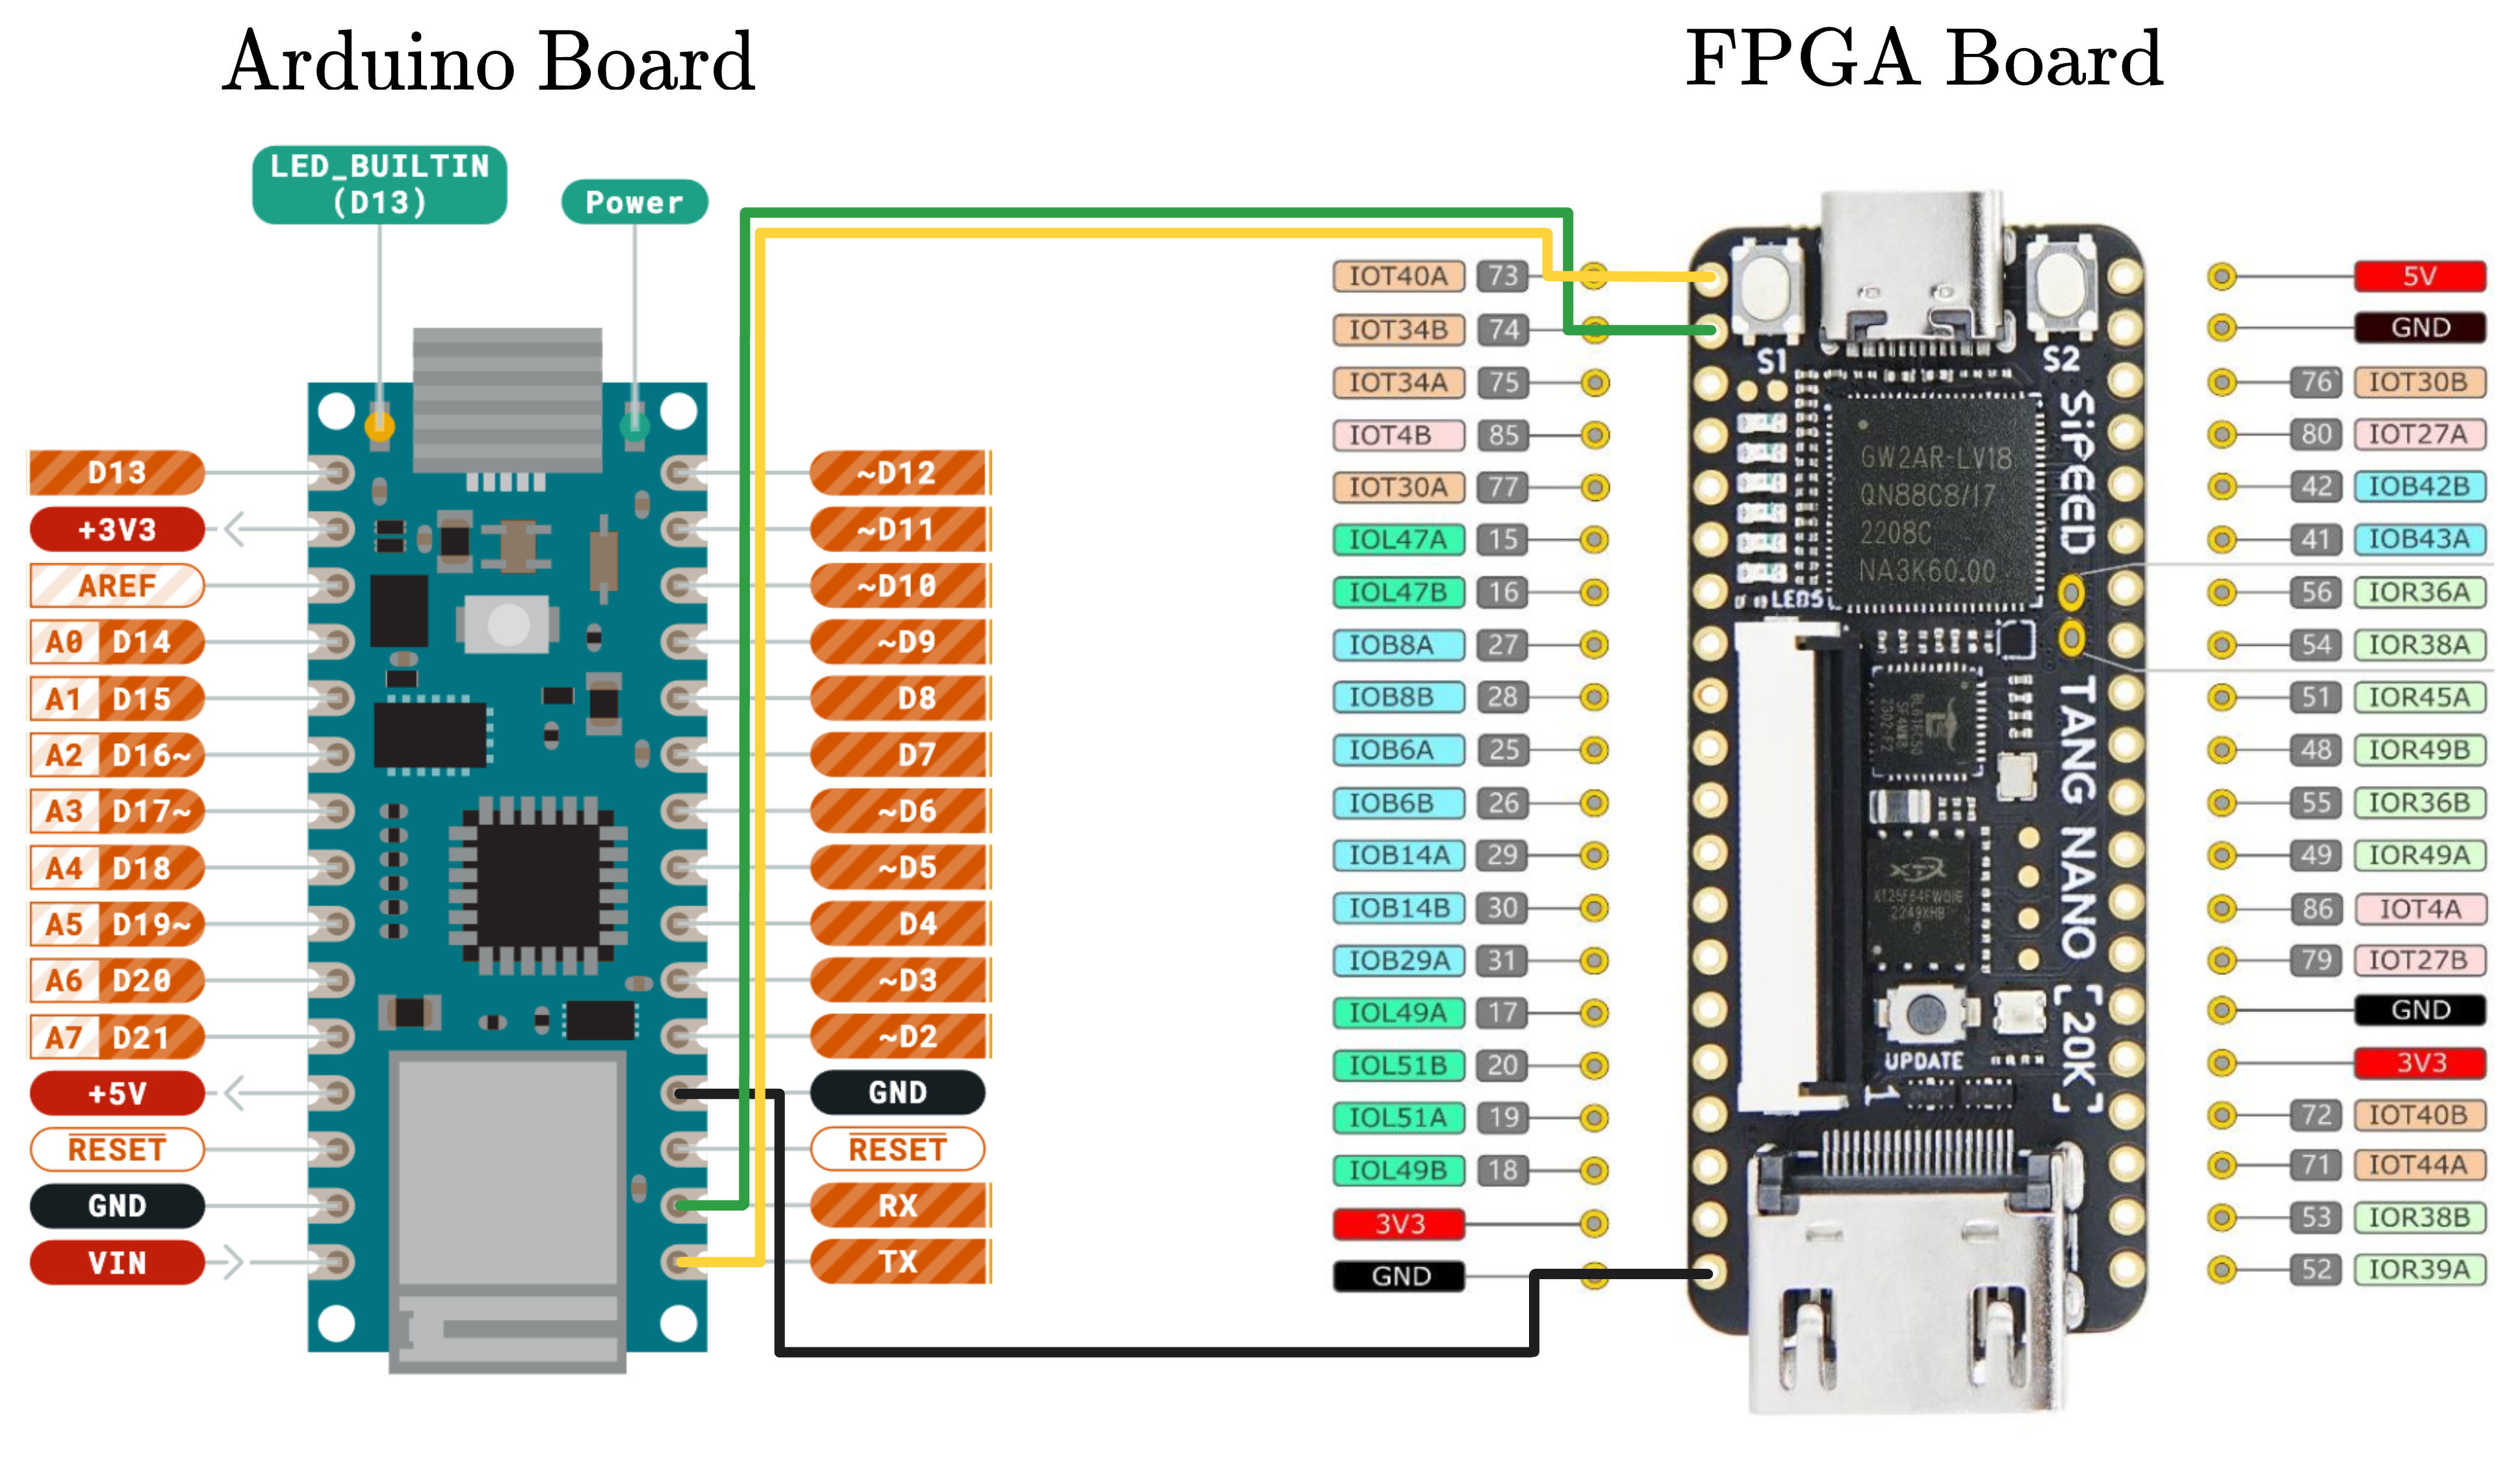
\includegraphics[width=1\linewidth]{img/arduino2fpga.png}
    \caption{UART connection between the Arduino board and the FPGA board}
    \label{fig:uart-arduino-fpga}
\end{figure}

The Arduino must communicate with the FPGA in order to manage the states and the LR-PUF and to carry out the necessary logic of the protocol. The FPGA and the Arduino exchange messages using a custom framing protocol layered on top of the UART.
Each frame has the structure shown in Table \ref{tab:proto-frame}.  There are two fields dedicated to the start-of-frame SOF1 and SOF2. This is done so as to reduce the probability of noise being taken as the start of a frame. Using only one field, that probability would be $1/256$, but with two fields it becomes $1/65536$ which is less likely. It also gives the parser the opportunity to re-synchronize after a corrupted or partial frame. A single SOF byte would not be reliable for this since it could randomly appear in corrupted data, but two consecutive bytes matching both SOF1 and SOF2 are less likely to appear.

The default Arduino RX and TX pins are connected to pins 74 and 73 of the FPGA board respectively, as seen in Figure \ref{fig:uart-arduino-fpga}.

\begin{table}[ht!]
\centering
\caption{FPGA protocol frame layout.}
\begin{tabular}{lll}
\hline
\textbf{Field} & \textbf{Size (bytes)} & \textbf{Description} \\
\hline
SOF1            & 1 & Start-of-frame marker (0xA5) \\
SOF2            & 1 & Start-of-frame marker (0x5A) \\
Version         & 1 & Protocol version (currently 1) \\
Message type    & 1 & REQ (1), RSP (2), or ERR (3) \\
Sequence number & 1 & Monotonically incrementing per call \\
Command         & 1 & Command identifier (Table~\ref{tab:proto-cmds}) \\
Payload length  & 2 & Little-endian, maximum 96 bytes \\
Payload         & 0--96 & Command-specific data \\
CRC16           & 2 & CRC-16/IBM over all fields after SOF \\
\hline
\end{tabular}
\label{tab:proto-frame}
\end{table}


The command identifiers used by the REPUSH-specific LR-PUF subsystem are listed in Table~\ref{tab:proto-cmds}. This is what the Arduino can tell the FPGA to do.

  \begin{table}[ht!]
  \centering
  \caption{LR-PUF commands descriptions}
  \begin{tabular}{cll}
  \hline
  \textbf{ID} & \textbf{Command} & \textbf{Purpose} \\
  \hline
  4  & \texttt{GET\_CA\_KEY}             & Retrieve the CA public key stored on the FPGA \\
  5  & \texttt{PUF\_GET\_FREE\_STATE}    & Return the index of an unoccupied state slot \\
  6  & \texttt{PUF\_RECONFIGURE\_STATE}  & Derive a new domain state $S^{Domain}_{i+1}$ \\
  8  & \texttt{PUF\_SET\_DOMAIN}         & Associate a domain string with a state slot \\
  9  & \texttt{PUF\_STORE\_ENROLLMENT}   & Write pubkey, challenge, and server key to a slot \\
  10 & \texttt{PUF\_SAVE\_STATES}        & Flush all state slots from RAM to SD card \\
  11 & \texttt{PUF\_FIND\_STATE\_BY\_DOMAIN} & Look up a slot by domain string \\
  12 & \texttt{PUF\_MARK\_ACKNOWLEDGED}  & Set the acknowledged flag for a slot / state \\
  13 & \texttt{PUF\_CLEAR\_STATES}       & Erase all state slots (debug use) \\
  14 & \texttt{PUF\_GET\_SLOT\_STATUS}   & Query the status and domain of a single slot / state \\
  15 & \texttt{PUF\_BCH\_ENROLL}         & Majority-vote PUF measurement and compute BCH helper data \\
  16 & \texttt{PUF\_BCH\_QUERY}          & Re-derive PUF response using BCH error correction \\
  \hline
  \end{tabular}
  \label{tab:proto-cmds}
  \end{table}

The structure of the payloads and responses of the commands can be found in table \ref{tab:proto-cmds-struct}. Some unused utility commands for debug purposes are also implemented and are found in table \ref{tab:proto-util-cmds}.

  \begin{table}[ht!]
  \centering
  \caption{LR-PUF commands payload and response structures (B stands for bytes)}
  \begin{tabular}{clll}
  \hline
  \textbf{ID} & \textbf{Command} & \textbf{Payload} & \textbf{Response} \\
  \hline
  4  & \texttt{GET\_CA\_KEY} & Empty & 32B pubkey \\
  5  & \texttt{PUF\_GET\_FREE\_STATE} & Empty & 1B state index \\
  6  & \texttt{PUF\_RECONFIGURE\_STATE} & State (1B) + seed (4B) & Empty \\
  8  & \texttt{PUF\_SET\_DOMAIN} & State (1B) + domain (var, max 63B) & Empty \\
  9  & \texttt{PUF\_STORE\_ENROLLMENT} & State + keys (81B total) & Empty \\
  10 & \texttt{PUF\_SAVE\_STATES} & Empty & Empty \\
  11 & \texttt{PUF\_FIND\_STATE\_BY\_DOMAIN} & Domain (var, max 63B) & 81B state data \\
  12 & \texttt{PUF\_MARK\_ACKNOWLEDGED} & State (1B) & Empty \\
  13 & \texttt{PUF\_CLEAR\_STATES} & Empty & Empty \\
  14 & \texttt{PUF\_GET\_SLOT\_STATUS} & State (1B) & Status (2B) + domain (max 63B) \\
  15 & \texttt{PUF\_BCH\_ENROLL} & State (1B) + ID (4B) + count (1B) & 32B enrolled key \\
  16 & \texttt{PUF\_BCH\_QUERY} & State (1B) + ID (4B) & 32B corrected key \\
  \hline
  \end{tabular}
  \label{tab:proto-cmds-struct}
  \end{table}


\begin{table}[ht!]
\centering
\caption{Utility commands}
\begin{tabular}{clll}
\hline
\textbf{ID} & \textbf{Command} & \textbf{Request} & \textbf{Response} \\
\hline
1 & \texttt{PING} & 4B string ``PING'' & Echo ``PING'' \\
2 & \texttt{GET\_INFO} & Empty & 8B+ (version, max payload, features) \\
3 & \texttt{GET\_TIME} & Empty & 4B timestamp \\
\hline
\end{tabular}
\label{tab:proto-util-cmds}
\end{table}

The Arduino initiates every exchange with a REQ frame and waits for a matching RSP or ERR frame identified by the same sequence number and command. 

An example request from the Arduino to the FPGA follows this sequence:
\begin{enumerate}
      \item The Arduino constructs a REQ frame which contains the command ID,
      a monotonically incrementing sequence number, and the command-specific payload.

      \item The Arduino flushes the UART RX buffer, sends the REQ frame, and enters a
      receive loop with a per-command timeout which ranges from one second for simple queries to 17 seconds for BCH enrollment with majority voting.

      \item The FPGA parses the incoming frame, validates the CRC, and executes the command.

      \item FPGA sends a response frame: either RSP on success or ERR on failure. The response carries the same sequence number
      and command ID as the request.

      \item Arduino's receive loop matches the response by checking
      \texttt{response.seq == request.seq} and \texttt{response.cmd == request.cmd}.
      Frames that do not match (e.g: stale output from a prior command) are discarded and
      the loop continues waiting. If the timeout expires without a matching frame, the
      Arduino retries with a fresh frame and a new sequence number, waiting
      150~ms before each retry. A maximum of 3 attempts are made in total, after which the call returns failure.
  \end{enumerate}

\subsection{Arduino Implementation}
The Arduino implementation is written in C++ and the PlatformIO IDE solution \cite{platformio_ide} was used for managing the project. The used Arduino board is an Arduino Nano 33 IoT \cite{arduino_nano_33_iot}.

\subsubsection{Commands}
The Arduino exposes the high-level commands in table \ref{tab:arduino-commands} via its USB serial interface, which DOMAN uses.

\begin{table}[ht!]
\centering
\caption{High-level commands from DOMAN to Arduino}
\begin{tabular}{lll}
\hline
\textbf{Command} & \textbf{Arguments} & \textbf{Purpose} \\
\hline
\texttt{enroll} & Certificate, Payload & Phase 1: Perform enrollment (Algorithm \ref{alg:dongle-enroll}) \\
\texttt{sign\_payload} & Domain, Payload & Phase 2: Sign non-sensitive request \\
\texttt{sign\_sensitive} & Domain, Payload & Phase 2: Sign sensitive request with user approval \\
\texttt{reconf} & Domain, Payload & Phase 3: Rotate key and reconfigure state \\
\texttt{acknowledge} & Domain, Signature & Phase 1: Acknowledge server-signed enrollment \\
\texttt{reconf\_ack} & Domain, Signature & Phase 3: Acknowledge server-signed reconfiguration \\
\texttt{ready} & — & Poll dongle availability (returns ``READY'') \\
\hline
\end{tabular}
\label{tab:arduino-commands}
\end{table}



In addition to the main protocol commands, the Arduino implements several debug commands for testing and development. The most commonly used state management debug commands are in table \ref{tab:debug-commands}.

\begin{table}[ht!]
\centering
\caption{State management debug commands}
\begin{tabular}{lll}
\hline
\textbf{Command} & \textbf{Arguments} & \textbf{Purpose} \\
\hline
\texttt{fp\_list\_states} & — & List all 11 state slots with their domain, \\
&  & initialization status, and acknowledgment flag \\
\texttt{fp\_clear\_states} & — & Erase all state slots from FPGA memory \\
&  & (resets dongle to factory state) \\
\hline
\end{tabular}
\label{tab:debug-commands}
\end{table}

\subsubsection{Cryptographic Schemes}
The Arduino implementation employs four cryptographic primitives:

\textbf{1. Ed25519: Edwards-Curve Digital Signature Algorithm}: A cryptographic signature scheme defined in RFC 8032 \cite{rfc8032}. The dongle uses the Ed25519 functions from the Arduino Cryptography Library \cite{arduinolibs_crypto}:
\begin{itemize}
    \item \texttt{Ed25519::sign(signature, privateKey, publicKey, message, messageLen)}: Signs a message with the private key.
    \item \texttt{Ed25519::verify(signature, publicKey, message, messageLen)}: Verifies a signature against a public key.
    \item \texttt{Ed25519::derivePublicKey(publicKey, privateKey)}: Derives the public key from a private key.
\end{itemize}
It is used during phase 1 to verify $[LoginPayload]_{SK_{\text{Server}}}$, to sign $[LoginPayload]_{SK_0}$ and verify the server's acknowledgment $LoginAck$. During phase 2, it is used to sign sensitive and non-sensitive requests $[SignaturePayload]_{SK_i}$ and $[SensitivePayload]_{SK_i}$. And during phase 3, to sign the reconfiguration token  ($[PK_{i+1} \| ReconfPayload]_{SK_i}$) and verify the server's acknowledgment $ReconfAck$.

\textbf{2. Curve25519 (X25519): Elliptic Curve Diffie-Hellman}: an elliptic curve designed for ECDH key agreement, defined in RFC 7748 \cite{rfc7748}. The following functions from the Arduino Cryptography Library are used:
\begin{itemize}
    \item \texttt{Curve25519::dh1(publicKey, privateKey)}: Generates the public key from a private key.
    \item \texttt{Curve25519::dh2(sharedSecret, privateKey)}: Computes the shared secret via scalar multiplication.
\end{itemize}
The exact usage for ECDH is explained in the next section below.

\textbf{3. ChaCha20-Poly1305: Authenticated Encryption with Associated Data (AEAD)}: A combined encryption and authentication scheme defined in RFC 7539 \cite{rfc7539}. It combines ChaCha20, which is a stream cipher, and Poly1305, which is a one-time authenticator. ChaCha20 handles confidentiality by encrypting the plain text and Poly1305 handles integrity by detecting if the cipher text was tampered with in-transit. The following functions from the Arduino Cryptography Library are used:
\begin{itemize}
    \item \texttt{ChaChaPoly::setKey(key, keyLen)}: Sets the 32-byte encryption key.
    \item \texttt{ChaChaPoly::setIV(iv, ivLen)}: Sets the 12-byte nonce.
    \item \texttt{ChaChaPoly::encrypt(ciphertext, plaintext, plaintextLen)}: Encrypts the plaintext.
    \item \texttt{ChaChaPoly::computeTag(tag, tagLen)}: Computes the 16-byte Poly1305 tag.
\end{itemize}
ChaCha20-Poly1305 is used during phase 1 to encrypt the $LoginToken$ and in phase 3 to encrypt the $ReconfToken$.

\textbf{4. SHA-256: Secure Hash Algorithm}: A cryptographic hash function defined in the FIPS 180-4 standard \cite{fips180_4}. The following functions from the Arduino Cryptography Library are used:
\begin{itemize}
    \item \texttt{SHA256::reset()}: Initializes the hash state.
    \item \texttt{SHA256::update(data, dataLen)}: Feeds data into the hash function (can be called multiple times for streaming).
    \item \texttt{SHA256::finalize(digest, digestLen)}: Completes the hash and returns the 32-byte digest.
\end{itemize}
SHA-256 is used for deriving the symmetric encryption key from the ECDH shared secret during phase 1 and phase 3 as explained in the next section below.




\subsubsection{Usage of ECIES (Elliptic Curve Integrated Encryption Scheme) for Encryption}
There is a slight deviation from the protocol design when it comes to encryption since the Ed25519 public key provided by the server $PK_{\text{Server}}^{\text{Ed25519}}$ can only be used for verifying signatures and not for encryption. Using ECIES we can use the provided server public key to encrypt a message that only the server could decrypt. ECIES is used during phase 1 to encrypt the $LoginToken$ and during phase 3 to encrypt the $ReconfToken$.

To explain how ECIES works in the technical implementation, the following notations are used:
\begin{itemize}
    \item $\text{Ed25519\_to\_X25519}(PK^{\text{Ed25519}})$: Function to convert an Ed25519 public key to X25519.
    \item $\text{X25519}(sk, pk)$: X25519 scalar multiplication to compute the shared secret from private key $sk$ and public key $pk$.
    \item $\text{SHA256}(m)$: SHA256 hash function.
    \item $\text{ChaCha20-Poly1305.Encrypt}(key, nonce, plaintext)$: ChaCha20 encryption with Poly1305 authentication.
    \item $\text{ChaCha20-Poly1305.Decrypt}(key, nonce, ciphertext, tag)$: ChaCha20 decryption with Poly1305 verification.
\end{itemize}

During phase 1, when the dongle needs to encrypt the $LoginToken$ which contains the username, password and $PK_0$ during $DongleEnroll$ (Algorithm \ref{alg:dongle-enroll}), it will follow the process described in the $ECIESEncrypt$ function defined in algorithm \ref{alg:ecies-encrypt-enroll}. It first takes the server's Ed25519 public key and converts it to an X25519 key suitable for ECDH (Elliptic Curve Diffie-Hellman), then it generates an ephemeral key pair, where the ephemeral public key is $eph\_pub=\text{X25519}(eph\_priv,G)$, with $G$ as the curve's base point. It then computes the ECDH shared secret as $shared\_secret=\text{X25519}(eph\_priv, PK_{\text{Server}}^{\text{X25519}})$, which is equivalent to $[a \cdot b]G$ where $a=eph\_priv$ and $b$ is the server's private scalar corresponding to its X25519 private key. The server will later be able to generate the shared secret using $shared\_secret=X25519(SK_{\text{Server}}, eph\_pub)$ due to the commutativity of elliptic curve scalar multiplication, in other words we would have:
$$
shared\_secret=\text{X25519}(a, [b]G) = \text{X25519}(b, [a]G) = [a \cdot b]G
$$
Where $a$ is the private scalar of the dongle and $b$ is the private scalar of the server.
Then a symmetric encryption key is derived by hashing the shared secret together with the ephemeral public key as $enc\_key=\text{SHA256}(shared\_secret||eph\_pub)$. Afterward, the plain text, which consists of the hex-encoded username, password and generated public key $PK_0$ separated by pipe characters, is encrypted using ChaCha20-Poly1305 with a randomly generated nonce, producing both a ciphertext and an authentication tag. Finally all sensitive intermediate values are deleted.

\begin{algorithm}[ht!]
\caption{$ECIESEncrypt(PK_{\text{Server}}^{\text{Ed25519}}, Username, Password, PK_0)$}
\begin{algorithmic}[1]
    \Require Server's Ed25519 public key $PK_{\text{Server}}^{\text{Ed25519}}$, user credentials $Username$ and $Password$, device generated public key $PK_{\text{0}}$.
    \Ensure  $(eph\_pub, nonce, ciphertext, tag)$ representing the encrypted LoginToken.

    \State $PK_{\text{Server}}^{\text{X25519}} \leftarrow \text{Ed25519\_to\_X25519}(PK_{\text{Server}}^{\text{Ed25519}})$

    \State $eph\_priv \leftarrow \text{TRNG}()$ \Comment{random 32-byte private key}
    \State $eph\_pub \leftarrow X25519(eph\_priv, \text{BasePoint})$ \Comment{derive public key}

    \State $shared\_secret \leftarrow \text{X25519}(eph\_priv, PK_{\text{Server}}^{\text{X25519}})$

    \State $enc\_key \leftarrow \text{SHA256}(shared\_secret \mathbin\| eph\_pub)$

    \State $plaintext \leftarrow \text{HexEncode}(Username) \,\|\, \texttt{"|"} \,\|\, \text{HexEncode}(Password) \,\|\, \texttt{"|"} \,\|\, \text{HexEncode}(PK_0)$

    \State $nonce \leftarrow \text{TRNG}()$ \Comment{12-byte IETF nonce}

    \State $(ciphertext, tag) \leftarrow \text{ChaCha20-Poly1305.Encrypt}(enc\_key, nonce, plaintext)$

    \State $\text{Wipe}(eph\_priv)$
    \State $\text{Wipe}(shared\_secret)$
    \State $\text{Wipe}(enc\_key)$
    \State $\text{Wipe}(plaintext)$

    \State \textbf{return} $(eph\_pub, nonce, ciphertext, tag)$
\end{algorithmic}
\label{alg:ecies-encrypt-enroll}
\end{algorithm}

The actual $LoginToken$ which will be transmitted to the server will have the following structure:
$$
LoginToken = eph\_pub \,\|\, nonce \,\|\, ciphertext \,\|\, tag
$$

The server decrypts the $LoginToken$ once it receives it during $VerifyLogin$ (Algorithm \ref{alg:verify-login}) by following the process outlined in $ECIESDecrypt$ (Algorithm \ref{alg:ecies-decrypt-enroll}). It begins by converting the server's Ed25519 private key to its X25519 equivalent and then reproduces the shared secret as $shared\_secret=\text{X25519}(SK_{\text{Server}}^{\text{X25519}},eph\_pub)$, which is equivalent to $[b \cdot a]G$ that is identical to the $[a \cdot b]G$ computed by the dongle as explained before. The symmetric key is then derived similarly as $enc\_key=\text{SHA256}(shared\_secret||eph\_pub)$. Decryption is then attempted using ChaCha20-Poly1305 and the authentication tag $auth\_valid$ is verified. If the tag check fails, the function fails to indicate that the token was tampered with in-transit. If the tag check is successful, the decrypted plain text is decoded to recover the username, password and $PK_0$. 

\begin{algorithm}[ht!]
\caption{$ECIESDecrypt(SK_{\text{Server}}^{\text{Ed25519}}, eph\_pub, nonce, ciphertext, tag)$}
\begin{algorithmic}[1]
    \Require Server's Ed25519 private key $SK_{\text{Server}}^{\text{Ed25519}}$, ephemeral public key $eph\_pub$, nonce, ciphertext, and authentication tag.
    \Ensure  Decrypted plaintext $(Username, Password, PK_0)$, or failure.
    \State $SK_{\text{Server}}^{\text{X25519}} \leftarrow \text{Ed25519\_to\_X25519}(SK_{\text{Server}}^{\text{Ed25519}})$
    \State $shared\_secret \leftarrow X25519(SK_{\text{Server}}^{\text{X25519}}, eph\_pub)$
    \State $enc\_key \leftarrow \text{SHA256}(shared\_secret \mathbin\| eph\_pub)$
    \State $(plaintext, auth\_valid) \leftarrow \text{ChaCha20-Poly1305.Decrypt}(enc\_key, nonce, ciphertext, tag)$
    \If{$auth\_valid = \textit{false}$}
        \State \textbf{return} ``Decryption failed: authentication tag verification failed''
    \EndIf
    \State $(Username, Password, PK_0) \leftarrow \text{HexDecode}(plaintext)$
    \State $\text{Wipe}(shared\_secret)$
    \State $\text{Wipe}(enc\_key)$
    \State \textbf{return} $(Username, Password, PK_0)$
\end{algorithmic}
\label{alg:ecies-decrypt-enroll}
\end{algorithm}

The same process for encrypting and decrypting is also used during phase 3 for encrypting and decrypting $ReconfToken$.

\subsubsection{Random Number Generation}
The Arduino must generate random numbers for three use-cases: the ephemeral keys for ECIES, nonces for ChaCha20-Poly1305 and for seeding the LR-PUF initial state $S_0$. Rather than relying on the Arduino's default weak \texttt{random()} function, another method was used.

The method was taken from \cite{rheingoldheavy2017better} and can be seen in the source code as the function \texttt{generateRandomSeed()}. It extracts randomness from an unconnected pin, in this case \texttt{A0} with the following steps:
\begin{enumerate}
    \item Read the analog pin 8 times and extract the least significant bit (LSB) of each reading
    \item Sum the 8 LSBs and take the parity (odd/even) as one random bit
    \item Assemble 8 parity bits into one byte
    \item Repeat 4 times to produce a 32-bit seed
\end{enumerate}

The entropy from thermal and electromagnetic noise on the unconnected analog pin is further amplified using this method. It is similar to how flipping a coin 8 times gives sequences that are less likely to be guessed.

\subsection{Touch Screen Implementation}
The dongle features a 2.4 inch TFT touch screen display with an ILI9341 display controller (Figure \ref{fig:tft-picture}). It has 240x320 pixels resolution in portrait orientation. The Arduino communicates with the display via SPI (Serial Peripheral Interface). As seen in table \ref{table:touchscreen-pins}, the SPI bus is shared between the display controller (ILI9341) and the touch controller (XPT2046) but the Arduino can choose which controller to address by pulling its CS (Chip select) line low. The touch screen implementation is initially based on the code from \cite{bytesnbits_spi_lcd_touchscreen}.

\begin{figure}
    \centering
    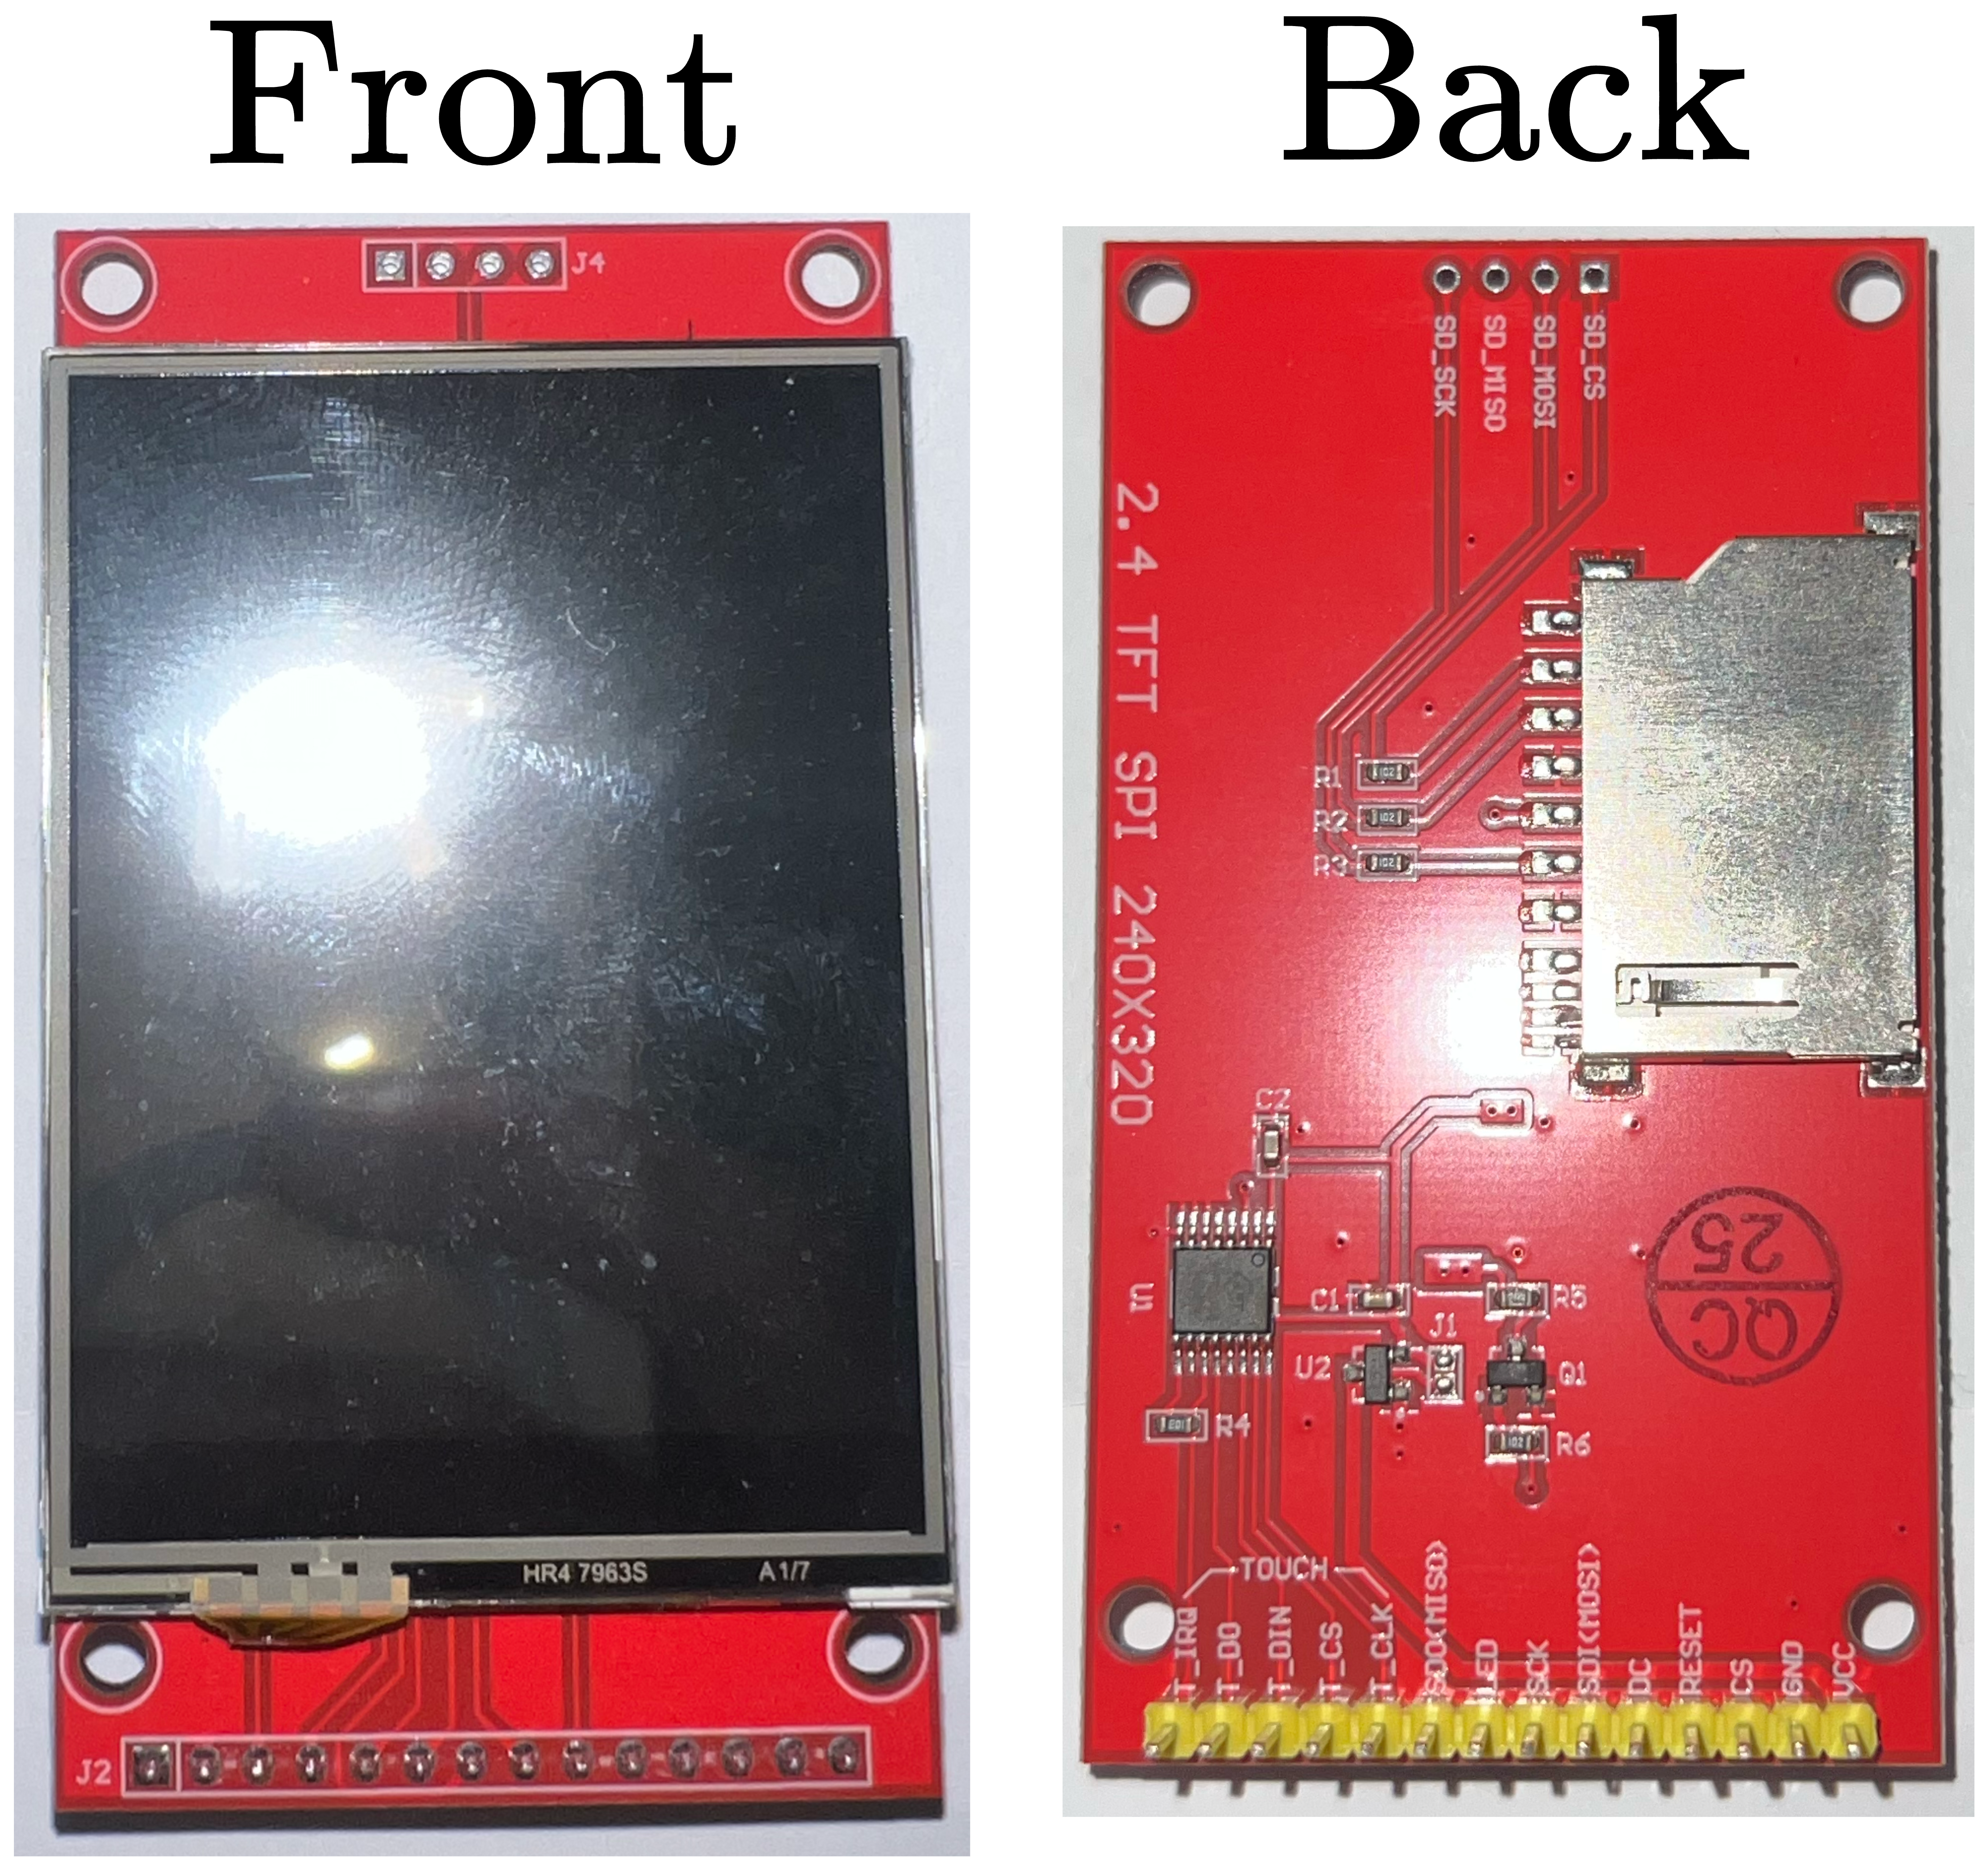
\includegraphics[width=0.5\linewidth]{img/touch-screen-picture.png}
    \caption{Pictures of the used TFT touch screen display}
    \label{fig:tft-picture}
\end{figure}

\begin{table}[ht!]
\centering
\caption{Pin assignments for display and touch controllers}
\begin{tabular}{|l|l|l|l|}
\hline
\textbf{Component} & \textbf{Function} & \textbf{Arduino Pin} & \textbf{Code Definition} \\
\hline
\multicolumn{4}{|c|}{\textbf{ILI9341 Display}} \\
\hline
\verb|VCC| & Power (3.3V) & \verb|3.3V| & — \\
\verb|GND| & Ground & \verb|GND| & — \\
\verb|LED| & LED Power (3.3V) & \verb|3.3V| & — \\
\verb|CS| & Chip Select & \verb|10| & \verb|TKB_TFT_CS| \\
\verb|D/C| & Data/Command & \verb|9| & \verb|TKB_TFT_DC| \\
\verb|RST| & Reset & \verb|8| & \verb|TKB_TFT_RST| \\
\verb|SDI(MOSI)| & SPI Data Out & \verb|11| & (Default SPI pin) \\
\verb|SDO(MISO)| & SPI Data In & \verb|12| & (Default SPI pin) \\
\verb|SCK| & SPI Clock & \verb|13| & (Default SPI pin) \\
\hline
\multicolumn{4}{|c|}{\textbf{XPT2046 Touch Controller}} \\
\hline
\verb|VCC| & Power (3.3V) & \verb|3.3V| & — \\
\verb|GND| & Ground & \verb|GND| & — \\
\verb|T_CS| & Chip Select & \verb|7| & \verb|TKB_TS_CS| \\
\verb|T_DIN| & SPI Data Out & \verb|11| & (Default SPI pin) \\
\verb|T_DO| & SPI Data In & \verb|12| & (Default SPI pin) \\
\verb|T_CLK| & SPI Clock & \verb|13| & (Default SPI pin) \\
\hline
\end{tabular}
\label{table:touchscreen-pins}
\end{table}

\subsubsection{Libraries}
The touch screen implementation uses the following Arduino libraries (see \verb|touch_keyboard.cpp|):
\begin{enumerate}
    \item \textbf{Adafruit GFX Graphic Library} \cite{adafruit_gfx_library}: Graphics library providing text, shapes, and drawing primitives.
    \item \textbf{Adafruit ILI9341 Library} \cite{adafruit_ili9341}: Display driver for the ILI9341 TFT controller.
    \item \textbf{XPT2046 Touchscreen Arduino Library} \cite{xpt2046_touchscreen}: Touch input driver for the XPT2046 controller.
    \item \textbf{FlashStorage Library} \cite{flashstorage}: Library for storing the calibration data on the non-volatile flash memory of the arduino.
    \item \textbf{SPI Library} \cite{arduino_spi_reference}: Standard Arduino SPI communication library.
\end{enumerate}

\subsubsection{Touch Screen Calibration}
Even though the resistive touch screen sits on top of the display, there is no shared circuitry between them, hence why we need to calibrate the touch screen to accurately map the touch coordinates coming from the touch screen to coordinates on the display. A resistive touch screen is comprised of two layers separated by a small gap, when a stylus is used to press somewhere on the screen, the two layers touch at that point, then by measuring two voltages $V_x$ and $V_y$, we get something similar to x-y coordinates (ADC readings).

During calibration, the XPT2046 touch controller provides 12-bit raw ADC readings (0--4095) at two reference points. The user is prompted to touch two crosshairs: one at the top-left corner (pixel 20,20) with ADC values $(x_1, y_1)$, and one at the bottom-right corner (pixel 210,300) with ADC values $(x_2, y_2)$. These ADC values are linearly mapped to accurate screen coordinates via affine transformations: 
$$\text{screen}_x = \frac{\text{rawADC}_x - c_x}{m_x}$$
$$\text{screen}_y = \frac{\text{rawADC}_y - c_y}{m_y}$$

The scaling factors are computed as:
$$m_x = (210 - 20) / (x_2 - x_1)$$
$$c_x = 20 - x_1 \cdot m_x$$
$$m_y = (300 - 20) / (y_2 - y_1)$$
$$c_y = 20 - y_1 \cdot m_y$$ 
These coefficients are stored in Arduino flash memory and applied to all subsequent touch inputs to convert raw ADC values to screen pixel coordinates. The screen calibration must only be done once since its results are stored on the flash memory to be reused on the next boot.


\subsubsection{User Interface Screens}

As seen in figure \ref{fig:screens-real}, the touch screen displays different screens during each phase to prompt the user. In the first phase, the user is prompted to initially approve the login by showing the server domain to make sure that the user will connect to the wanted server and not some other malicious domain (Screen (a)), if the user clicks on "ACCEPT", they are prompted to enter their username and password using the on-screen keyboard (Screens (b) and (c)) and then screen (d) is shown to confirm the receipt of the credentials. During phase 2, if the user makes a sensitive request that needs signing, screen (e) appears where the description of the sensitive request is shown and the user can choose to accept it or reject it. During phase 3, the user is prompted with screen (f) to accept or reject the session renewal. All screens are rendered using the Adafruit GFX Graphic Library to draw text, shapes, and buttons. As explained before, user interaction occurs through the resistive touch screen, where touches are read via SPI communication and then converted from 12 bit ADC values to accurate pixel coordinates using the stored affine transformations. The touch coordinates are then compared against the bounding boxes to determine which button was selected and execute the necessary action.

\begin{figure}
    \centering
    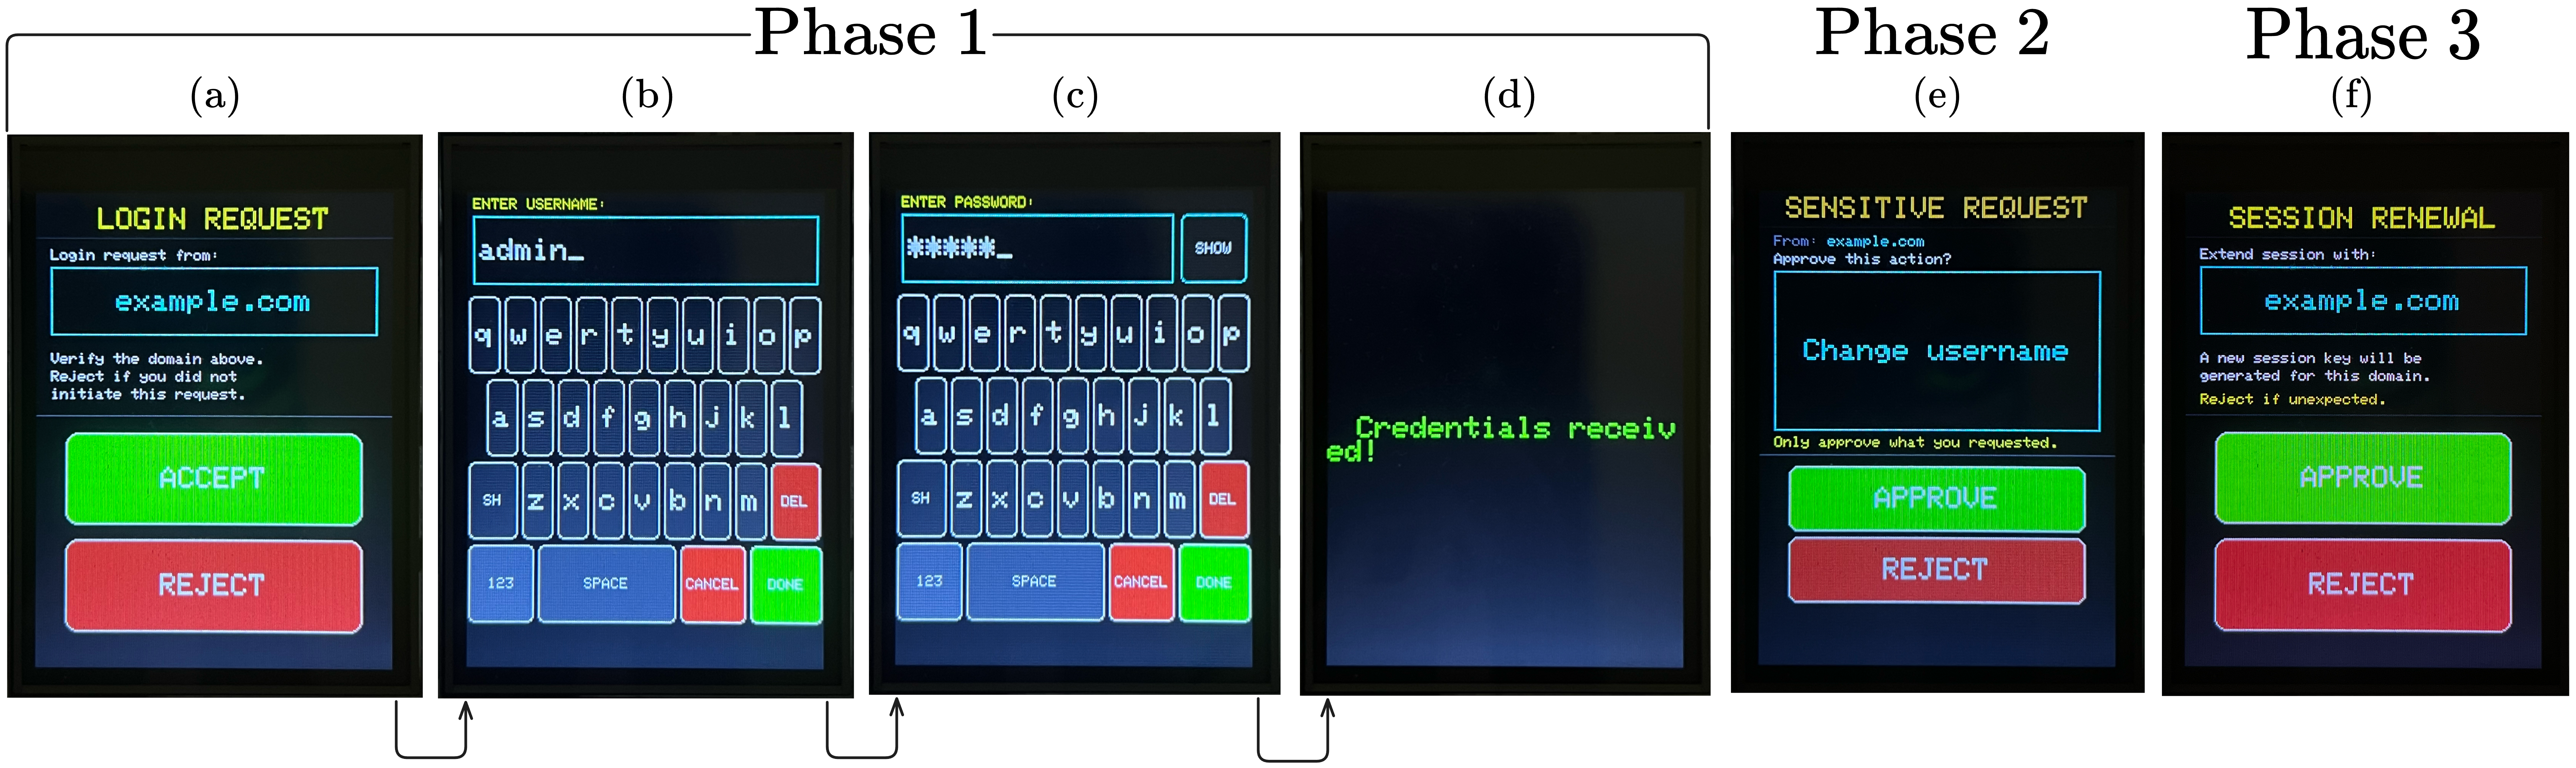
\includegraphics[width=1.1\linewidth]{img/screens-real.png}
    \caption{Pictures of all the possible screens}
    \label{fig:screens-real}
\end{figure}
  
\section{DOMAN Implementation}
DOMAN (Dongle Manager) is implemented as a local FastAPI \cite{fastapi_docs} server that exposes a WebSocket \cite{rfc6455} endpoint at \texttt{ws://127.0.0.1:8765/ws} to the browser. It simply translates JSON commands from the browser into newline-terminated ASCII commands and sends them to the Arduino over the USB CDC serial port. For example, a signature request arrives from the browser to DOMAN over the WebSocket as:
\begin{verbatim}
{
  "cmd":         "sign_payload",
  "domain":      "...",
  "payload_b64": "..."
}
\end{verbatim}
and is forwarded to the Arduino as the newline-terminated ASCII string:
\begin{verbatim}
sign_payload <domain> <payload>\n
\end{verbatim}

DOMAN uses an asynchronous event loop (\verb|asyncio|) for all WebSocket and HTTP handling, while serial communication runs in a dedicated thread since the blocking serial IO would otherwise block the event loop. 

Since the dongle can only process one request at a time, concurrent requests are serialised using a lock so that only one command is sent to the dongle at a time.

WebSocket was chosen over a conventional HTTP endpoint because dongle operations are long-running and produce incremental output. An HTTP response would have to buffer the entire operation before returning, leaving the browser with no feedback during the wait, or the browser could continuously poll DOMAN, both approaches are not ideal. A WebSocket connection however allows DOMAN to forward each output line from the dongle to the browser as it arrives, giving the user real-time progress of each phase.

DOMAN also exposes two HTTP debug endpoints for testing purposes: \texttt{GET /debug/list-states} to list all LR-PUF state slots on the FPGA and \texttt{POST /debug/clear-states} to erase them. A Swagger UI at \verb|http://127.0.0.1:8765/docs| can be used to easily call these endpoints (Figure \ref{fig:swaggerUI}).

\begin{figure}
    \centering
    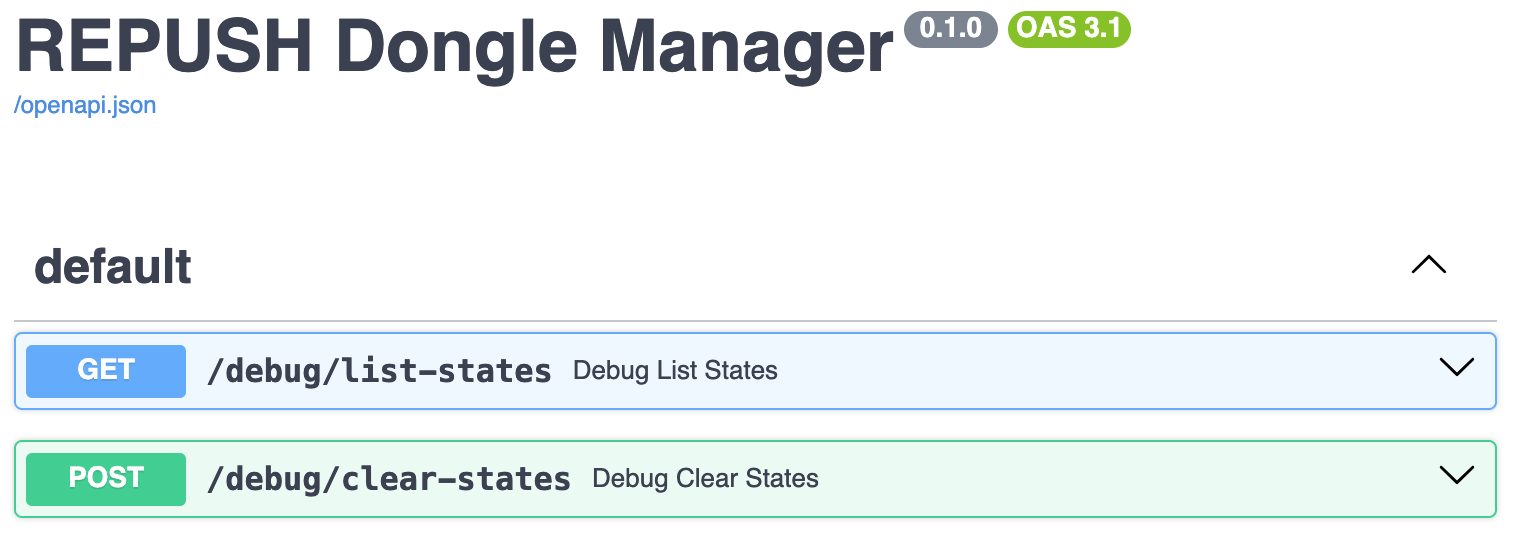
\includegraphics[width=1\linewidth]{img/swaggerUI-DOMAN.png}
    \caption{DOMAN Swagger UI}
    \label{fig:swaggerUI}
\end{figure}
As mentioned in the design section, DOMAN does not perform any cryptographic operations. It simply acts as a translation and orchestration layer between the browser and the dongle. The DOMAN implementation can be found in the repository named \verb|REPUSH-DOMAN|.

\section{Browser / Frontend Implementation}

The browser frontend is an HTML page served statically by the REPUSH server which contains all the necessary JavaScript to allow the browser to communicate and coordinate with DOMAN via the previously mentioned WebSocket endpoint. For this implementation, the page is intended as a demonstration of the protocol, as such, it is very explicit and transparent about the three phases and their inner workings, as seen in figure \ref{fig:landing-page}. A production website would perform most of these steps silently in the background. For styling the page, Tailwind CSS \cite{tailwindcss} was used.
\begin{figure}
    \centering
    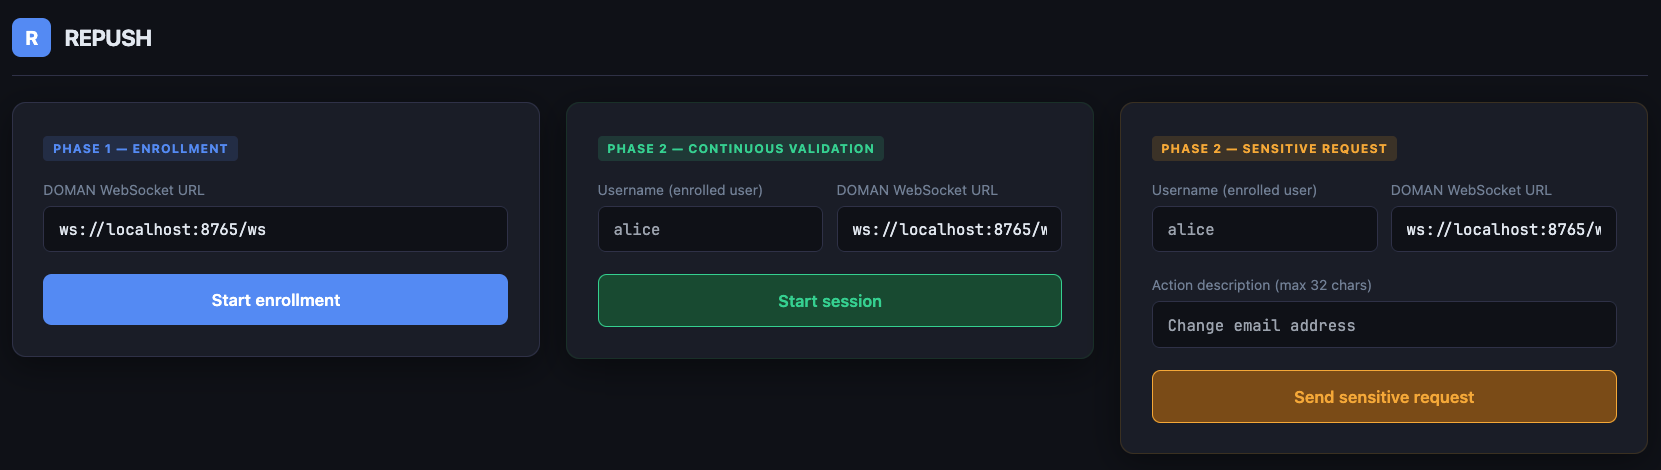
\includegraphics[width=1\linewidth]{img/landing-page.png}
    \caption{REPUSH demonstration page}
    \label{fig:landing-page}
\end{figure}

The page is divided into three side-by-side panels:
\paragraph{Phase 1 panel:} It accepts the DOMAN WebSocket URL as input and triggers the enrollment on the dongle when the user clicks on "Start enrollment". The JavaScript calls the REPUSH server with \texttt{POST /api/enroll/init} to obtain the certificate and enrollment payload from the server, then forwards them to the dongle via DOMAN. The user then has to approve the login request on the touch screen for the server's domain and enter their credentials on the dongle. The dongle's output is then sent back to the server on \texttt{POST /api/enroll/verify} so that the server can verify the credentials and continue accordingly by returning the acknowledgment. This acknowledgment is then returned to the dongle via DOMAN. If the acknowledgment on the dongle is successful, the enrollment is finalized by calling \texttt{POST /api/enroll/confirm}, after which the frontend immediately requests a phase 2 session token via \texttt{POST /api/session/start} and holds it in memory as a JavaScript variable. No cookies are set for this demonstration, rather session continuity is maintained purely through this variable. The final state of the panel after a successful enrollment can be seen in figure \ref{fig:phase-1-panel}. In "EVENT LOG", each output line from the dongle is appended to the log panel in real time with a timestamp as it arrives over the WebSocket connection. Each dongle command follows a self-contained lifecycle: the frontend opens a WebSocket connection to DOMAN, sends the JSON command, and appends each incoming line to the log panel until DOMAN sends a terminal message indicating the command has completed, at which point the connection is closed. The log also contains events from the server.

\begin{figure}
    \centering
    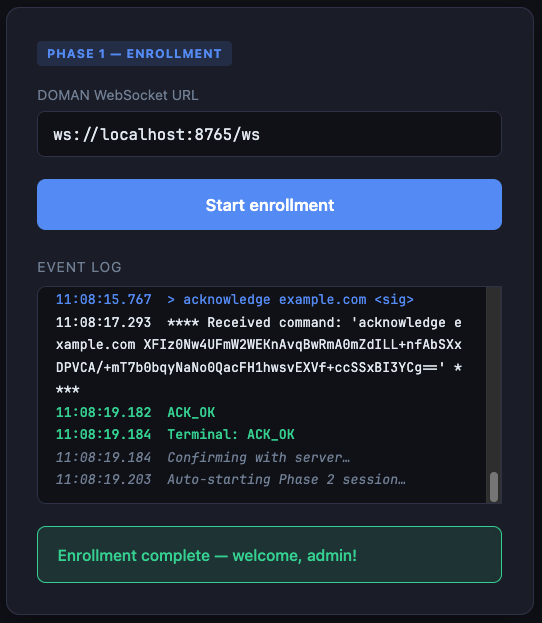
\includegraphics[width=0.5\linewidth]{img/phase-1-panel.png}
    \caption{Phase 1 panel after successful enrollment}
    \label{fig:phase-1-panel}
\end{figure}

\paragraph{Phase 2 and 3 panel:} This panel shows two live progress bars updated every 500 ms by polling \texttt{GET /api/session/status}. As seen in figure \ref{fig:phase-2-panel}, the first bar shows the elapsed time since the last revalidation relative to $T_\text{Validity}$, when this bar is full, on the subsequent request, the dongle will be asked to sign a non-sensitive payload for proof of ownership. The second bar below shows the age of the session relative to $T_\text{Expiry}$, when this bar is full, on the subsequent request, the dongle will prompt the user to extend the session and new keys will be generated for the new session. The "Make request" button simulates a non-sensitive request by calling \texttt{POST /api/session/ping}. The server may respond with \texttt{ok}, \texttt{revalidation\_required}, or \texttt{reconfiguration\_required}. If revalidation is required, the browser forwards the non-sensitive payload to the dongle via DOMAN and submits the resulting signature to the server by calling \texttt{POST /api/session/submit\_signature}. If reconfiguration is needed, the browser sends the reconfiguration payload to the dongle and submits the resulting token by calling \texttt{POST /api/session/verify\_reconf}, delivers the acknowledgment back to the dongle and finalizes the session renewal by calling \texttt{POST /api/session/confirm\_reconf} which replaces the session token with a new one. Since the session only expires every 300 seconds, the button "Force reconfig now" can be used to make it expire sooner for demonstration purposes. The "EVENT LOG" contains timestamped logs from both the server and the dongle. 

\begin{figure}
    \centering
    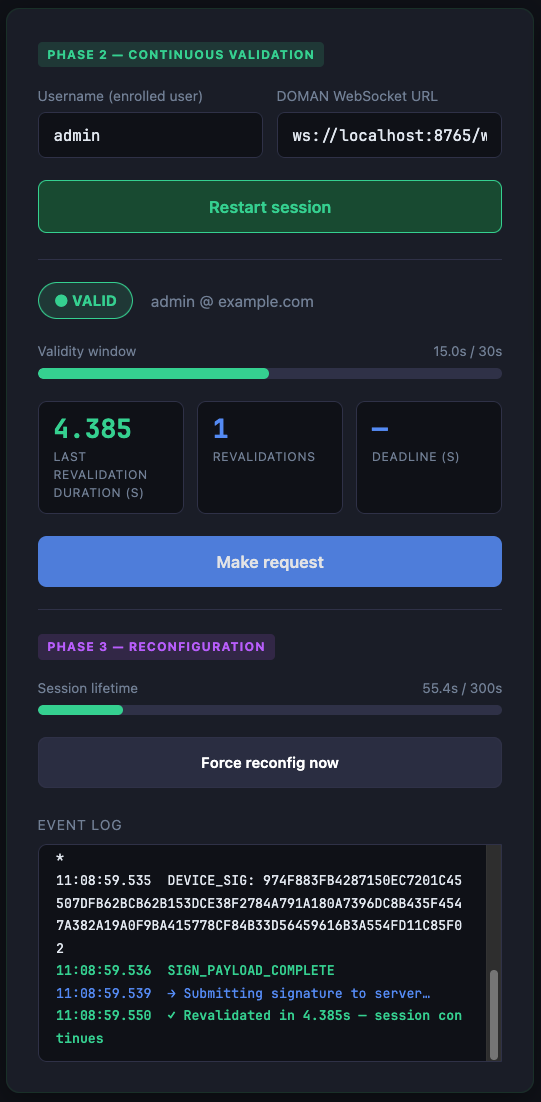
\includegraphics[width=0.5\linewidth]{img/phase-2-panel.png}
    \caption{Phases 2 and 3 panel after the session starts}
    \label{fig:phase-2-panel}
\end{figure}

\paragraph{Sensitive request panel:} The third panel (Figure \ref{fig:phase-2-sensitive-panel}) allows for testing a sensitive signing request. The username is auto-filled after enrollment and the tester can specify which message to show on the dongle. In a real use-case, this would be handled by the server, not by the  user in the frontend. The frontend calls \texttt{POST /api/sensitive/request} to obtain a sensitive payload from the server, then the dongle prompts the user with the sensitive action and its description and submits the resulting signature accordingly to \texttt{POST /api/sensitive/verify}. The "EVENT LOG" shows the real-time progress from the dongle and server.

\begin{figure}
    \centering
    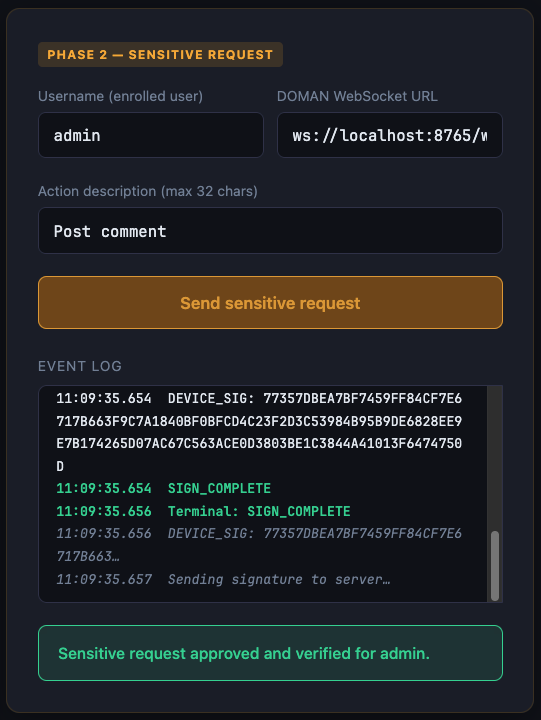
\includegraphics[width=0.5\linewidth]{img/phase-2-sensitive-panel.png}
    \caption{Phase 2 sensitive request panel after a successful signature request}
    \label{fig:phase-2-sensitive-panel}
\end{figure}

\section{Server / Backend Implementation}

The REPUSH server is a FastAPI \cite{fastapi_docs} server written in Python. For demonstration purposes, it runs locally, but in a real setting, it would be a remote server.

\subsection{Libraries}
The server implementation relies on the following Python libraries:

\begin{enumerate}
  \item \textbf{FastAPI} \cite{fastapi_docs}: Server framework used to define all API endpoints and handle request validation.
  \item \textbf{SQLAlchemy} \cite{sqlalchemy}: ORM (Object-Relational Mapping) used to manage the SQLite enrollment database and abstract all database operations.
  \item \textbf{pyca/cryptography} \cite{pycryptography}: Provides the server-side implementations of Ed25519 signing and verification, X25519 Diffie-Hellman, and ChaCha20-Poly1305 authenticated encryption used in the ECIES construction.
  \item \textbf{pyca/bcrypt} \cite{bcrypt}: Used to hash and verify user passwords stored in the database.
  \item \textbf{Pydantic} \cite{pydantic}: Handles request and response schema validation for all API endpoints.
\end{enumerate}



\subsection{State and Storage}
The server stores durable enrollment records such as the username, password hash, enrolled dongle public key $PK_i$, domain and the session challenge $C^i_\text{Session}$ in a SQLite \cite{sqlite} database under a table called \texttt{users} (Table \ref{tab:db-schema-users}). When phase 2 starts, $PK_i$ and $C^i_\text{Session}$ are copied from the database into a global dict which uses session tokens as its keys. This dict also contains all the necessary timestamp variables to determine if a revalidation or reconfiguration is due. The three global time parameters that control the frequency of validations and reconfigurations are defined as: 
\begin{itemize}
  \item $T_{\text{Validity}}$ (default 30 seconds): maximum interval between dongle revalidations.
  \item $T_{\text{Timeout}}$ (default 60 seconds): grace window for the dongle to respond before the session is terminated.
  \item $T_{\text{Expiry}}$ (default 300 seconds): maximum session lifetime before a full Phase~3 reconfiguration is required.
\end{itemize}


\begin{table}[ht!]
\centering
\caption{\texttt{users} SQL table schema.}
\begin{tabular}{ll}
\hline
\textbf{Field} & \textbf{Description} \\
\hline
\texttt{username}      & Primary identifier \\
\texttt{password\_hash} & Bcrypt-hashed password \\
\texttt{device\_pubkey} & Enrolled Ed25519 public key $PK_i$ (hex) \\
\texttt{domain}        & Enrolled domain string \\
\texttt{challenge\_hex} & Raw session challenge $C^i_{\text{Session}}$ (hex) \\
\texttt{enrolled\_at}  & Timestamp of the most recent enrollment or reconfiguration \\
\texttt{created\_at}   & Timestamp of account creation \\
\hline
\end{tabular}
\label{tab:db-schema-users}
\end{table}

\subsection{Phase 1: Enrollment and Login}
The following endpoints are used to implement the enrollment phase:
\begin{itemize}
    \item \texttt{POST /api/enroll/init}: generates a fresh certificate and signed login payload, storing the session challenge in memory.
    \item \texttt{POST /api/enroll/verify}: receives and decrypts the login token using the ECIES construction, cross-checks the dongle public key, verifies the device signature, authenticates the username and password against the database, and returns the acknowledgment signature.
    \item \texttt{POST /api/enroll/confirm}: finalizes enrollment by writing the dongle public key and session challenge to the database. 
\end{itemize}
\subsection{Phase 2: Operation}
The following endpoints are used to implement the second phase:
\begin{itemize}
    \item \texttt{POST /api/session/ping}: used to simulate a non-sensitive request. It checks $T_{\text{Expiry}}$ first: if the session has exceeded its lifetime, it returns \texttt{reconfiguration\_required} with a reconfiguration payload. Otherwise, if $T_{\text{Validity}}$ has elapsed since the last revalidation, it returns \texttt{revalidation\_required} with a signed non-sensitive payload and starts a termination countdown. If neither threshold is reached, it returns \texttt{ok}. When a revalidation is needed, a background task is scheduled to terminate the session after $T_{\text{Timeout}}$ seconds.
    \item \texttt{POST /api/session/submit\_signature}: verifies the dongle's Ed25519 signature and, on success, cancels the termination task and resets the last-validation timestamp.
    \item \texttt{POST /api/sensitive/request}: builds and signs a sensitive payload carrying the action description.
    \item \texttt{POST /api/sensitive/verify}: verifies the dongle's signature on the sensitive payload before authorizing the action.
\end{itemize}
\subsection{Phase 3: Reconfiguration}
\begin{itemize}
    \item \texttt{POST /api/session/verify\_reconf}: decrypts the reconfiguration token, verifies the device's signature over $PK_{i+1}$ using the old $PK_i$, and issues the reconfiguration acknowledgment.
    \item \texttt{POST /api/session/confirm\_reconf}: writes the new device public key and session challenge to the database, issues a new session token, and retires the old one. 
    \item \texttt{POST /api/session/force\_reconfig}:  resets the session start time so that the next ping immediately triggers $T_\text{Expiry}$, allowing the reconfiguration to be tested on demand without waiting for $T_\text{Expiry}$ to elapse.
\end{itemize} 

\subsection{CA Implementation}
In this implementation, the server also acts as the Certificate Authority. The CA private key is loaded from a local key file at startup alongside the server's own key pair. When \texttt{POST /api/enroll/init} is called, the server constructs a 128-byte certificate by concatenating the zero-padded domain string and its own Ed25519 public key, then signing the result with the CA private key. In a real use-case, the CA would be a separate offline entity rather than the server itself.






% !TeX encoding = UTF-8
% !TeX spellcheck = en_GB
% !TeX root = ../thesis.tex

\chapter{Evaluation and Discussion}
\label{chapter:evaluation}
This chapter evaluates the REPUSH protocol and its proof-of-concept implementation. In doing so, it addresses research question 3 by evaluating the security of the protocol and comparing it to the original PUSH protocol, and it covers research question 4 by measuring the performance of the implementation. 

\section{Security Evaluation}
\subsection{Adversary Model}
The security evaluation follows the threat model outlined in chapter \ref{chapter:design}. The adversary $\Adv$ is assumed to have arbitrary code execution on the host machine. $\Adv$ can read from and write to any memory accessible to the browser and DOMAN, intercept and tamper with inter-process communication, make requests on behalf of the user, and steal session cookies. The communication channel between the browser and the server is also treated as under $\Adv$'s control. However, $\Adv$ is assumed to be incapable of physically interacting with the dongle device and is assumed to computationally be bounded, i.e. unable to break the cryptographic operation within a reasonable time frame.   

This adversary model is stronger than the one considered by the original PUSH protocol \cite{10.1007/978-3-032-07894-0_7}, which only considered browser compromise. REPUSH assumes the entire host is compromised, with the exception of the dongle and server, which are considered as trusted and safe.

\subsection{Resistance to Common Attacks}

\paragraph{Sniffing Attack:}
By monitoring all traffic between protocol parties, $\Adv$ may observe public data such as the challenge issued by the server $C^i_\text{Session}$, $PK_\text{Server}$, cookies, nonces and signed payloads. Notably, the dongle-generated public keys $PK_i$ are never transmitted in plain-text. They are always encrypted so that only the server can decrypt them. None of this data enables $\Adv$ to maintain a session independently of the dongle. Continuing a session requires a periodic validation with a fresh dongle signature, which in turn requires knowledge of $SK_i$, which is never exposed to the host. Moreover, each signature request includes a fresh server-generated nonce that prevents replay attacks.

\paragraph{Cookies Theft and XSS Attacks:} The primary attack against session security is cookie theft, which is carried out by malware (Infostealers). Although XSS was historically a common method for stealing cookies, modern browsers mitigate this through the \verb|HttpOnly| flag, which prevents JavaScript from accessing cookie values directly. The dominant way of stealing cookies is therefore malware which has code execution on the host. In REPUSH, stolen cookies alone are insufficient to hijack a session. Since every time $T_\text{Validity}$ is elapsed, the server requests a fresh signature to verify ownership of the dongle. Without the dongle, $\Adv$ cannot produce the necessary signed payload. The attacker can therefore only use cookies within the $T_\text{Validity}$, and the usage is limited to non-sensitive requests. Real attackers are more interested in using the cookies for sensitive requests like changing passwords and emails, such a sensitive request requires a user-approved dongle signature independent of $T_\text{Validity}$, which makes them inaccessible to $\Adv$.

\paragraph{Replay Attack:}
Each $SignaturePayload$ and $SensitivePayload$ includes a fresh nonce $N$ generated by the server at the time of the request. Even if $\Adv$ records a previously signed payload, replaying it would fail as the server would reject the consumed nonce. Furthermore, the $T_\text{Timeout}$ deadline further restricts the window within which the valid signed payload must arrive at the server.

\paragraph{Man-in-the-Middle (MitM) Attack:}
During phase 1, the dongle verifies the server's certificate using the CA's public key. The verified domain is then displayed on the dongle's screen, where the user must read it and explicitly approve it. A MitM adversary who would use their own certificate must forge the CA's signature, which is infeasible under the assumed adversary model. In subsequent phases, the server signs every payload with $SK_\text{Server}$, so the dongle would only sign payloads coming from the server.

\paragraph{Silent Signing Attack:} The main attack motivating the design of REPUSH is the silent signing attack. In PUSH, $\Adv$ with code execution on the host could silently intercept server-generated payloads and relay them to the dongle via PUFMAN to obtain valid signatures without any user awareness. REPUSH explicitly considers DOMAN as untrusted and addresses this in two ways depending on the type of request. For non-sensitive requests, the dongle verifies the server's signature on $SignaturePayload$ before signing it. $\Adv$ therefore cannot craft an arbitrary payload for the dongle to sign. However $\Adv$ may still intercept the server-generated payload and forward it to the dongle to obtain a signature that it can forward to persist the stolen session. This attack is possible, but only for non-sensitive requests. For sensitive requests, the dongle requires explicit user approval on the dongle display before signing $SensitivePayload$, $\Adv$ can therefore not trigger a silent signature since any attempt to do so would immediately make the user reject it since it would be unsolicited.

\paragraph{Passive Compromise Detection:} A direct consequence of the trusted display requirement for sensitive requests is that REPUSH provides a passive out-of-band indicator of compromise. If any malware attempts to use the dongle to sign a sensitive request that the user did not initiate, an unexpected prompt appears on the dongle's screen, which would immediately alert the user. Because the dongle is isolated from the host and only exposes a limited interface of commands, even the most privileged malware cannot bypass the user-approval on the dongle's screen. This gives the user a reliable way of detecting intrusion independently of any host-based security solution.

\paragraph{Enrollment Hijacking Attack:} In PUSH, if the browser is compromised before enrollment, $\Adv$ could redirect the enrollment to bind the session to their own dongle. REPUSH eliminates this attack by having the dongle independently verify the server certificate and display the domain on the screen for the user to verify it. Furthermore, the credentials are entered on the dongle and not on the browser and are encrypted in transit. A compromised browser can therefore neither alter the domain nor intercept the credentials.

\paragraph{Impersonation Attack:} To impersonate the dongle, $\Adv$ must produce valid signatures to the provided payload using the private key $SK_i$ associated with the currently enrolled public key $PK_i$. This requires knowledge of $SK_i$ which is derived inside the dongle and is never stored on or exposed to the host. Physical access to the dongle could allow the attacker to get $SK_i$, but as mentioned earlier, it is not considered in the attacker model. This limitation will be discussed later in the limitations section. 

\paragraph{Device Capturing and Cloning:}
Although physical attacks are outside our scope, REPUSH's use of an LR-PUF offers many advantages in the case of dongle cloning. Even if the attacker were to steal the dongle and enumerate all the CRPs of the CHOICE-PUF, the attacker would still not be able to predict future keys because the seeds depend on the states as well as the CHOICE-PUF responses, and the states have a TRNG element and time-stamp that determine them. Therefore the attacker would not be able to predict future ($SK_i$,$PK_i$) pairs that the dongle could generate.

\paragraph{Denial-of-Service (DoS) Attack:}
Any party in the REPUSH protocol can be the target of a DoS attack, but the impact is limited to compromising accessibility and no more than that. DoS attacks are less of an issue when it comes to hardware dongles compared to servers, since if that were to occur then that means there is malware on the host. An attacker would have no incentive to just deny service to the dongle since that immediately tells the user that the host is infected.

\section{CHOICE-PUF Evaluation}

In this section, we evaluate the statistical properties of the CHOICE PUF implementation. All measurements were collected via the default serial interface of the FPGA over USB-C at 115200 baud rate. Two datasets were collected. The first dataset is used for uniformity and bit independence evaluation. It consists of one 64-bit response per valid challenge, which gives 184 responses containing a total of $184\times64=11776$ measured bits. The second dataset is used for reliability and error-correction evaluation. It consists of 1000 responses per valid challenge, which gives a total of 184000 measurements. All responses are raw outputs of the PUF before any error correction or majority voting is applied.

\subsection{Uniformity}
A PUF with ideal uniformity produces responses in which each bit is equally likely to be a 0 or a 1. When this property holds, the responses are deemed unpredictable. The ideal uniformity is 50\%, i.e. half of the bits are 0 and the other half are 1. Significant deviations from this ideal indicate a bias on the PUF which could simplify attacks.

\subsubsection{Per-bit Uniformity}
Per-bit uniformity measures the uniformity of each individual bit position across the set of all valid challenges.  For each bit position $b \in \{0, \ldots, 63\}$, the fraction of challenges in which that bit is equal to 1 is computed as:
$$
U_b = \frac{1}{n} \sum_{i=1}^{n} r_i[b]
$$
where $n=184$ is the number of valid challenges and $r_i[b] \in \{0,1\}$ is the $b$-th bit of the $i$-th response. The ideal value is $U_b=0.5$.

The mean per-bit uniformity $\bar{U}_\text{per-bit}$ is the mean of $U_b$ over all bits, which is computed as:
$$
    \bar{U}_\text{per-bit} = \frac{1}{64} \sum_{b=0}^{63} U_b
$$

The measured mean per-bit uniformity is $\bar{U}_\text{per-bit}=51.04\%$, which is very close to the ideal $50\%$.

The mean absolute deviation (MAD) measures on average how far each bit position deviates from the ideal uniformity:
$$
MAD = \frac{1}{64}\sum_{b=0}^{63}|U_b - 0.5|
$$

The measured MAD is $MAD=6.33\%$.

Figure \ref{fig:per-bit-uniformity} shows the per-bit uniformity for all 64 bit positions. The bars in red deviate by 10 percentage points or more from the ideal 50\% uniformity.

\begin{figure}
    \centering
    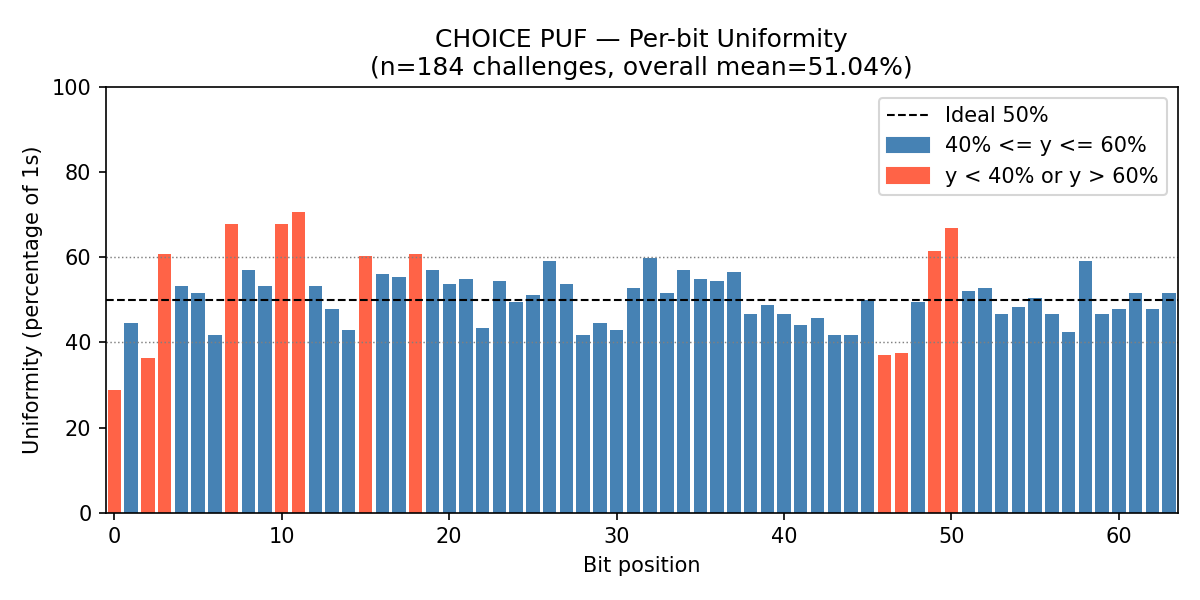
\includegraphics[width=1\linewidth]{img/plot_uniformity_bits.png}
    \caption{CHOICE-PUF: Per-bit Uniformity.}
    \label{fig:per-bit-uniformity}
\end{figure}

The most biased bit is bit position 0, which equals 1 in only 28.8\% of responses. But overall, the other bits are well balanced. Per-bit uniformity captures whether bit positions are uniform across all challenges, but it does not reveal whether individual responses are uniform. The next section addresses this. 

\subsubsection{Per-challenge Uniformity}
Per-challenge uniformity measures the Hamming weight of each 64-bit response as:
$$
U_i = \frac{1}{64}\sum_{b=0}^{63} r_i[b]
$$
where $r_i[b] \in \{0,1\}$ is the $b$-th bit of response $r_i$. The ideal value is $U_i=0.5$ for every challenge. 

The mean per-challenge uniformity $\bar{U}$ is the mean of $U_i$ over all responses, which is computed as:
$$
\bar{U} = \frac{1}{n}\sum_{i=1}^{n} U_i
$$
where $n = 184$ is the number of valid challenges. It was measured as $\bar{U}=51.04\%$.

The per-challenge MAD measures on average how far each individual response deviates from the ideal uniformity:
$$
MAD_\text{per-challenge} = \frac{1}{n}\sum_{i=1}^{n}|U_i - 0.5|
$$

The measured value is $MAD_\text{per-challenge} = 27.86\%$

Figure \ref{fig:per-challenge-uniformity}  shows the per-challenge uniformity sorted in ascending order. Only 22 out of the 184 challenges (12\%) fall near the ideal 50\% uniformity; those are highlighted in blue on the figure. Despite the ideal-looking mean uniformity, the responses are in majority quite far from the mean as can be seen with the red bars. This shows that the CHOICE PUF alone is not a reliable source of uniform responses, with 88\% of challenges producing outputs far from the ideal. Naively selecting a challenge at random would most likely yield a biased response. This reinforces the need for the LR-PUF construction to augment the CHOICE-PUF's responses using hashing with random states.

\begin{figure}
    \centering
    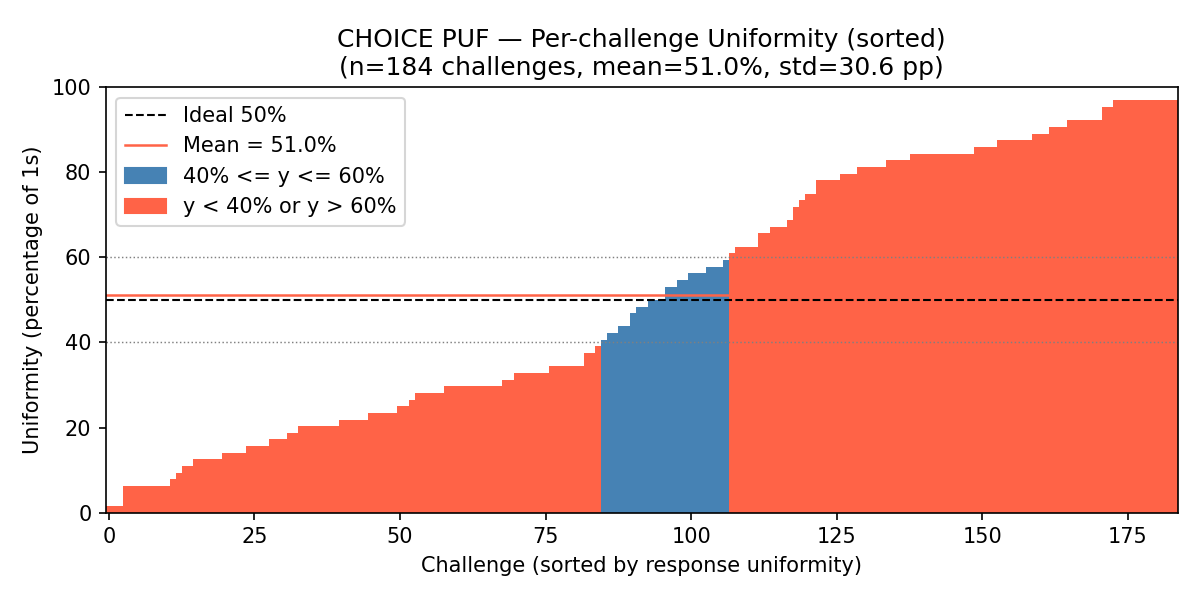
\includegraphics[width=1\linewidth]{img/plot_uniformity_per_challenge.png}
    \caption{CHOICE-PUF: Per-challenge Uniformity}
    \label{fig:per-challenge-uniformity}
\end{figure}

Table \ref{tab:uniformity-results} summarizes the uniformity results. $\bar{U}$ and $\bar{U}_\text{per-bit}$ are identical by definition. The mean absolute values however differ. $MAD_\text{per-challenge} = 27.86\%$ is much bigger than $MAD_\text{per-bit}=6.33\%$. This shows that individual bit positions are moderately balanced whilst individual bit sequences are heavily skewed. 

\begin{table}[ht!]
\centering
\caption{CHOICE PUF uniformity results summary.}
\begin{tabular}{llll}
\hline
\textbf{Metric} & \textbf{Symbol} & \textbf{Measured} & \textbf{Ideal} \\
\hline
Mean per-bit uniformity            & $\bar{U}_\text{per-bit}$      & 51.04\%          & 50\%  \\
MAD per-bit                               & $MAD_\text{per-bit}$   & 6.33\%         & 0\% \\
Bit positions within $\pm10\%$\   & —                             & 52 / 64 (81\%)   & 100\% \\
Bit positions outside $\pm10\%$  & —                             & 12 / 64 (19\%)   & 0\%   \\
\hline
Mean per-challenge uniformity      & $\bar{U}$                           & 51.04\%          & 50\%  \\
MAD per-challenge                              & $MAD_\text{per-challenge}$   & 27.86\%        & 0\% \\
Challenges within $\pm10\%$      & —                                   & 22 / 184 (12\%)  & 100\% \\
Challenges outside $\pm10\%$     & —                                   & 162 / 184 (88\%) & 0\%   \\
\hline
\end{tabular}
\label{tab:uniformity-results}
\end{table}

\subsection{Uniqueness}

Uniqueness measures how distinct the responses of two or more different PUF instances are when presented with the same challenge. The standard metric for measuring uniqueness is the inter-device Hamming distance, which has an ideal value of 50\%, meaning that two independent devices agree on exactly half of the bits by randomness. A score significantly below 50\% indicates that responses are too similar across devices, which would allow one device to impersonate another.

Measuring inter-device uniqueness requires multiple FPGA chips flashed with the PUF design, which is impractical for this thesis. To circumvent this limitation, the 64-bit response is split into two 32-bit responses $r^{lo}$ and $r^{hi}$, and the two responses are treated as coming from two different devices. For each challenge $i$, the inter-device Hamming distance is computed as:
$$
D_i = \frac{1}{32}\sum_{b=0}^{31} \left| r_i^\text{hi}[b] - r_i^\text{lo}[b] \right|
$$
where $r_i^\text{hi}[b]$ and $r_i^\text{lo}[b]$ are the $b$-th bit of each half.

The mean uniqueness score $\bar{D}$ is averaged across all $n = 184$ challenges:
$$
\bar{D} = \frac{1}{n} \sum_{i=1}^{n} D_i
$$

The measured mean uniqueness is $\bar{D} = 29.50\%$.

The mean absolute deviation of the uniqueness from the ideal is:
$$
MAD_\text{uniqueness} = \frac{1}{n} \sum_{i=1}^{n} |D_i - 0.5|
$$

The measured value is $MAD_\text{uniqueness} = 21.28\%$

Figure \ref{fig:uniqueness} shows the inter-device Hamming distance for each challenge sorted in ascending order. Only 53 out of the 184 valid challenges (28.8\%) fall near the ideal 50\% uniqueness, which tells us that the two halves do not fully behave as two different devices.

\begin{figure}
    \centering
    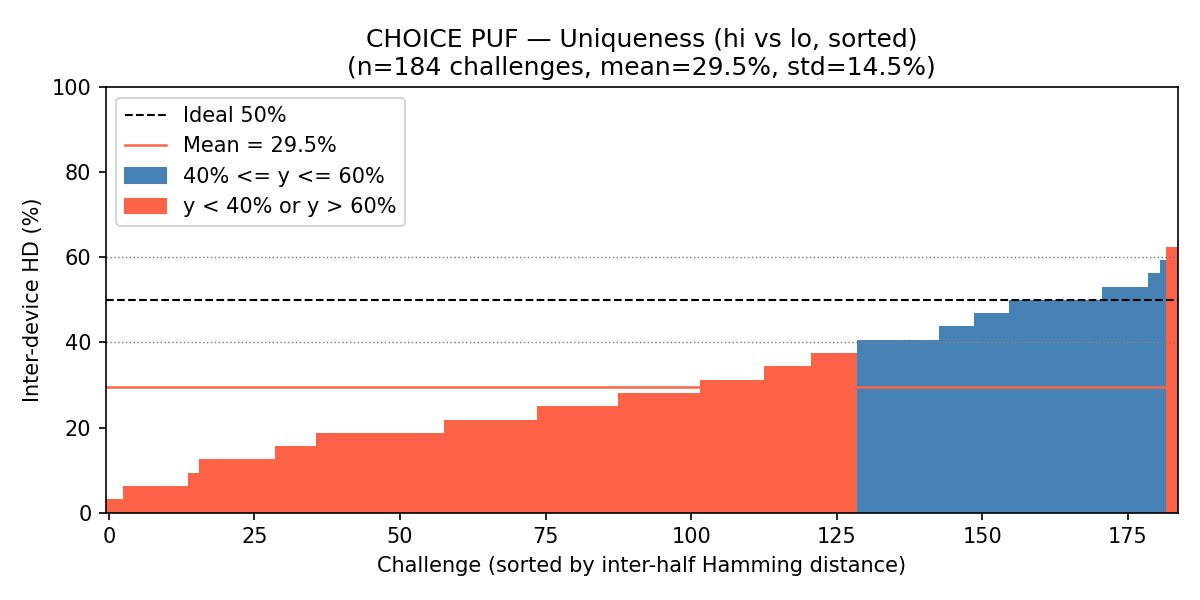
\includegraphics[width=1\linewidth]{img/plot_uniqueness.png}
    \caption{CHOICE-PUF: Uniqueness}
    \label{fig:uniqueness}
\end{figure}

Table \ref{tab:uniqueness-results} summarizes the uniqueness results. The mean uniqueness of $\bar{D} = 29.50\%$ is well below the ideal of 50\%, and the large $MAD_\text{uniqueness} = 21.28\%$ confirms that individual challenges deviate substantially from the ideal. This is explained by the structural proximity of the two halves on the FPGA. This measurement can therefore only be considered as a lower bound rather than a true inter-device uniqueness score. A rigorous evaluation would require measuring uniqueness over many boards.


\begin{table}[ht!]
\centering
\caption{CHOICE PUF uniqueness results summary.}
\begin{tabular}{llll}
\hline
\textbf{Metric} & \textbf{Symbol} & \textbf{Measured} & \textbf{Ideal} \\
\hline
Mean inter-half distance           & $\bar{D}$                         & 29.50\%          & 50\%  \\
MAD                                & $MAD_\text{uniqueness}$           & 21.28\%          & 0\%   \\
Challenges within $\pm10\%$        & —                                 & 53 / 184 (29\%)  & 100\% \\
Challenges outside $\pm10\%$       & —                                 & 131 / 184 (71\%) & 0\%   \\
\hline
\end{tabular}
\label{tab:uniqueness-results}
\end{table}




\subsection{Reliability}
Reliability measures how consistently a PUF produces the same response when queried with the same challenge under the same conditions. A PUF usually produces slightly different responses on each query due to changing conditions. For the REPUSH protocol, reliability is important since the BCH fuzzy commitment scheme can only tolerate up to $T=4$ bit flips between the enrollment response and the query response. If the PUF produces more than 4 flipped bits, BCH decoding will fail, and the key cannot be reconstructed.

The reliability metric used is the one from the pypuf python library \cite{nils_wisiol_2021_5222515}. Each challenge is queried $r$ times, producing $r$ 64-bit responses. Let $\hat{p}_b$ be the fraction of $r$ responses in which bit position $b$ equals 1. The reliability of bit $b$ under some challenge is:
$$
\rho_b = \hat{p}_b^2 + (1-\hat{p}_b)^2 = 1 - 2\hat{p}_b(1-\hat{p}_b) = 1 - 2\,\mathrm{Var}(\hat{p}_b)
$$

$\rho_b$ is the probability that two independent queries of the same challenge agree on bit $b$. Both queries return 1 with probability $\hat{p}_b^2$ and both return 0 with probability $(1-\hat{p}_b)^2$. After expanding this expression we get $\rho_b = 1 - 2\hat{p}_b(1-\hat{p}_b)$ where $\hat{p}_b(1-\hat{p}_b)$ is the variance of a binary random variable. Reliability is simply 1 minus twice the observed variance of the bit. A perfectly stable bit ($\hat{p}_b \in \{0,1\}$) gives $\rho_b = 1$ and a maximally noisy bit ($\hat{p}_b = 0.5$) gives $\rho_b = 0.5$.

The dataset has $r=1000$ samples per challenge across all $n=184$ valid challenges. The responses are arranged into an $(n \times 64 \times r)$ array. For each of the challenge-bit pairs, $\hat{p}_b$ is computed as the fraction of 1s across the $r=1000$ queries. Then $\rho_b$ is computed using the formula above. The result is an $(n \times 64)$ reliability matrix which gives the reliability of each bit given a challenge.

From the reliability matrix, we compute the per-bit reliability by averaging the reliability for each bit $b$ over all $n$ challenges:

$$
\bar{\rho}_b = \frac{1}{n} \sum_{i=1}^{n} \rho_{i,b}
$$

As seen in figure \ref{fig:reliability-per-bit}, the least reliable bit is bit position 1 with a reliability of 98.39\%. The majority of bit positions have above 99\% reliability which indicates that the CHOICE-PUF is very reliable.

\begin{figure}
    \centering
    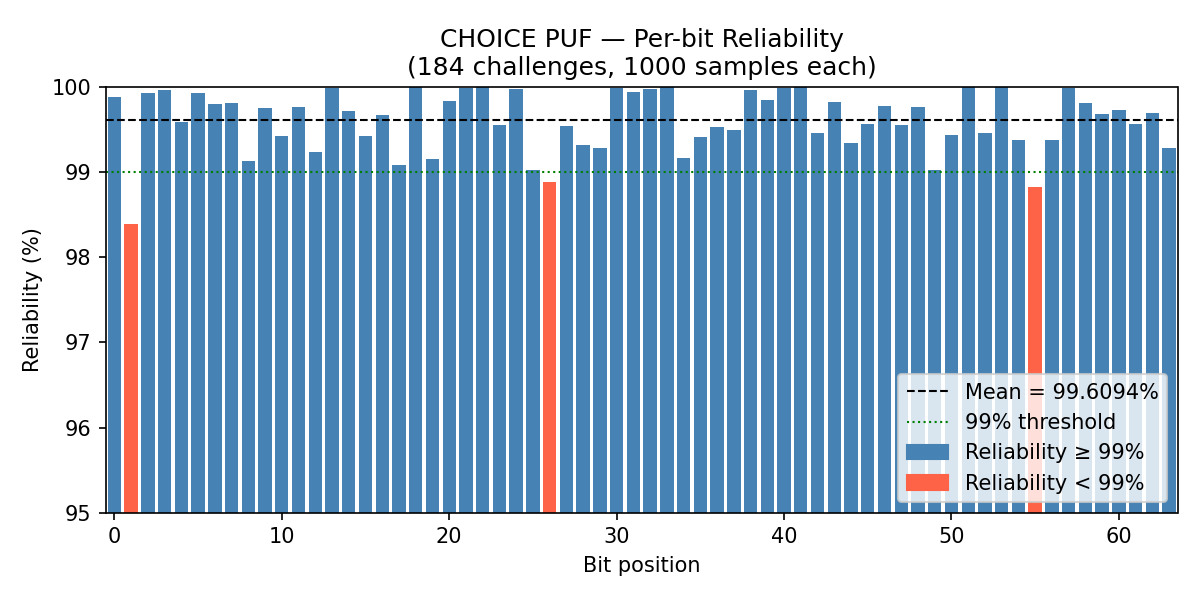
\includegraphics[width=1\linewidth]{img/plot_reliability_per_bit.png}
    \caption{CHOICE-PUF: Per-bit Reliability}
    \label{fig:reliability-per-bit}
\end{figure}

Alternatively, the per-challenge reliability can be computed by averaging over all 64 bits for each challenge to give one reliability value per challenge $i$:

$$
\bar{\rho}_i = \frac{1}{64} \sum_{b=0}^{63} \rho_{i,b}
$$

As seen in figure \ref{fig:reliability-per-challenge}, the least reliable challenge has a reliability of 97.41\%, whilst most challenges are well above 99\%. 

\begin{figure}
    \centering
    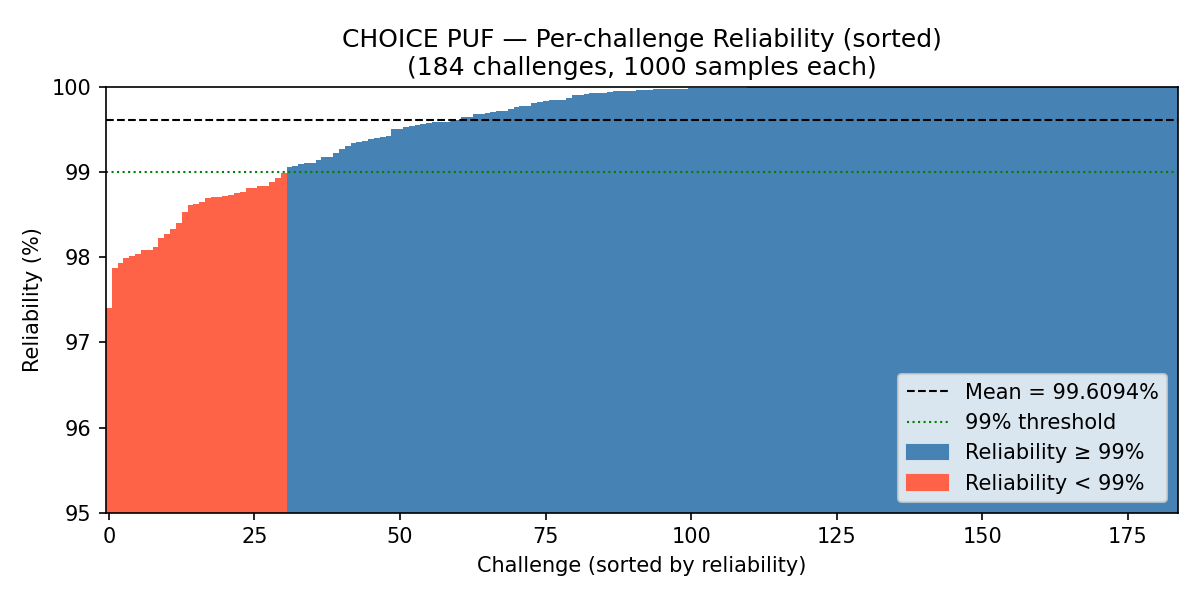
\includegraphics[width=1\linewidth]{img/plot_reliability_per_challenge.png}
    \caption{CHOICE-PUF: Per-challenge Reliability}
    \label{fig:reliability-per-challenge}
\end{figure}

The overall reliability $\bar{\rho}$ is the average of all values within the reliability matrix: 
$$
\bar{\rho} = \frac{1}{64n} \sum_{i=1}^{n} \sum_{b=0}^{63} \rho_{i,b}
$$
The measured value for the overall reliability is $\bar{\rho}=99.61\%$

Table \ref{tab:reliability-results} summarizes the reliability results.

\begin{table}[ht!]
\centering
\caption{CHOICE PUF reliability results summary.}
\begin{tabular}{llll}
\hline
\textbf{Metric} & \textbf{Symbol} & \textbf{Measured} & \textbf{Ideal} \\
\hline
Overall reliability              & $\bar{\rho}$          & 99.61\%   & 100\% \\
Least reliable bit (bit 1)       & $\min_b \bar{\rho}_b$ & 98.39\%   & 100\% \\
Least reliable challenge (idx 99)& $\min_i \bar{\rho}_i$ & 97.41\%   & 100\% \\
\hline
\end{tabular}
\label{tab:reliability-results}
\end{table}

\section{LR-PUF Evaluation}

The statistical properties of the CHOICE-PUF evaluated in the previous section carry directly over to the LR-PUF. The high $99.61\%$ reliability of the CHOICE-PUF ensures that the BCH fuzzy commitment can consistently reconstruct the same seed across repeated queries since the expected number of bit flips per query is within the $T=4$ correction capacity. The poor per-challenge uniformity of the CHOICE-PUF responses, where 88\% of the challenges are 10\% far from the ideal 50\% uniformity, is fixed by the BLAKE2b hash that is applied on the CHOICE-PUF responses since by definition a cryptographic hash function produces uniform outputs regardless of the bias in its inputs. Therefore, the 32-byte seed derived from the LR-PUF is uniformly distributed. The LR-PUF inherits the reliability of the CHOICE-PUF while eliminating its uniformity limitations through hashing. Inter-state uniqueness within one device is guaranteed by the random seed that is used to generate each state. But inter-device uniqueness remains dependent on the CHOICE-PUF producing distinct responses on different FPGA chips, which we could not fully verify.

\subsection{TRNG Evaluation}
A critical piece to the LR-PUF is the TRNG used for generating the initial state. In the implementation, a seed is generated from an unconnected pin on the Arduino. It is therefore essential to evaluate the randomness of the outputs generated by this method. To assess the quality of this source, 125\,000 bytes (1\,000\,000 bits) were collected and evaluated using the NIST SP800-90B non-IID entropy assessment tool (\cite{nist_sp800_90b} and \cite{sp800_90b_entropy_assessment}).

Min-entropy $H$ represents the worst-case unpredictability of a random source. It describes the unpredictability of an outcome determined solely by the probability of the most likely result \cite{crypto_se_63797}. It is defined as:
$$
H = -\log_2(p_{\max})
$$

where $p_{\max}$ is the probability of the most likely output value.

For example, if we have an algorithm that produces 8-digit passwords, if the number \verb|00000000| occurs 50\% of the time, and the remaining $10^8-1$ passwords occur with equal probability, then the min-entropy is $H=-\log_2(P(X=\texttt{00000000}))=-\log_2(0.5)=1$.
Equivalently, $p_{\max} = 2^{-H}$. Therefore a min-entropy of 1 means that there is a 50\% chance that a single guess gets the right password. Whilst a min-entropy of 8 means only 1 in 256 guesses would get it right ($H = -\log_2\left(\tfrac{1}{256}\right) = -\log_2(2^{-8}) = 8$). This assumes the attacker knows the distribution and exploits it. Rather than enumerating passwords at random, the attacker always guesses \texttt{00000000} first and succeeds 50\% of the time in a single try. If the distribution were perfectly uniform, no single guess would be better than any other and the min-entropy would be $-\log_2(1/10^8) \approx 26.6$ bits, which means that even an optimal attacker only has a 1-in-100-million chance on the first guess.

The NIST SP800-90B non-IID entropy assessment tool assesses this entropy. It does so under the non-IID assumption. IID stands for independent and identically distributed. A source is IID if every sample is drawn independently from the same fixed distribution. For example, throwing a coin is an IID source since one coin toss does not influence the next in any way. But the successive readings of a floating Arduino pin are non-IID since every reading is somewhat influenced by the previous one. The assessment tool therefore does not assume that the entropy source is IID and applies many tests to estimate the min-entropy.

The tool produced the following estimates:
\begin{itemize}
    \item $H_\text{original}=7.571$ bits per byte. The tool was told that each sample is 8 bits long, so it treats each byte as a single symbol and estimates its min-entropy. A perfectly random byte would have $H_\text{original}=8$ bits, i.e. each of the 256 values is equally likely. The measured value of 7.571 means that the source provides   $\frac{7.571}{8}\cdot100\%=94.6\%$ of that 8-bit maximum.
    \item $H_\text{bitstring}=0.825$ bits per bit. Here, each bit is considered as a symbol rather than the entire byte. A perfectly random bit would have $H_\text{bitstring}=1$ bit, i.e. an equal probability of 1 and 0 ($p_{\max}=0.5$). The measured value of 0.825 means $p_{\max} = 2^{-0.825} \approx 0.567$, so the tool can predict the next bit correctly $56.7\%$ of the time using its predictors. This is only possible if the predictors find some sort of pattern in the previous bits, which means that consecutive bits are not fully independent from each other.    
\end{itemize}

To compare these two estimates and get a more conservative minimum entropy, $H_\text{bitstring}$ is multiplied by 8 to convert it to "bits per byte" $8\cdot H_\text{bitstring}=6.603$ and the minimum of the two measured values is taken as the actual min-entropy:
$$
H=  \min\!\left(H_\text{original},\ 8 \times H_\text{bitstring}\right) = \min(7.571,\ 6.603) = 6.603 \text{ bits/byte.}
$$


The 32-byte seed generated by the TRNG for initializing the LR-PUF state therefore carries around $32 \cdot 6.603 \approx 211$ bits of min-entropy. The theoretical maximum would be 256 bits of min-entropy. Despite falling short of full entropy, the 211 bits of min-entropy are usable for cryptographic purposes, since an optimal adversary who exploits the full distribution of the source succeeds with probability of at most $2^{-211}=3.04\times10^{-64}$.

Table \ref{tab:trng-results} summarizes the findings.

It should be noted that the SP800-90B standard recommends a minimum of 1\,000\,000 bytes of measurements for getting statistically meaningful results, whereas we only collected 125\,000 bytes due to the low throughput of using \texttt{analogRead} for the TRNG ($\approx$15\,bytes per second).

\begin{table}[h]
\centering
\caption{NIST SP\,800-90B entropy assessment results for the Arduino floating-pin TRNG.}
\begin{tabular}{lcc}
\hline
\textbf{Metric} & \textbf{Measured} & \textbf{Ideal} \\
\hline
$H_\text{original}$ (bits/byte) & 7.571 & 8 \\
$H_\text{bitstring}$ (bits/bit) & 0.825 & 1 \\
$8 \times H_\text{bitstring}$ (bits/byte) & 6.603 & 8 \\
$H = \min(H_\text{original},\ 8 \times H_\text{bitstring})$ (bits/byte) & \textbf{6.603} & 8 \\
Total min-entropy for 32-byte seed (bits) & $\approx 211$ & 256 \\
\hline
\end{tabular}
\label{tab:trng-results}
\end{table}

\section{Performance Evaluation}
\subsection{LR-PUF Performance}
To measure the performance of the LR-PUF implementation, latency was measured from the host computer using a Python script that communicates with the FPGA via its default serial interface of USB-C at 115200 baud rate. To record the time taken, the start time is taken from the moment the command was transmitted until the final response line is received. The reported measurements therefore include a small additional delay introduced by the UART communication.

\subsubsection{BCH Enroll}

Each enrollment sample covers the total time for the following major operations:
\begin{itemize}
    \item $1\times$ BLAKE2b hash: for running the $map_{in}$ function.
    \item $10\times$ CHOICE-PUF query: to do majority voting and get a stable CHOICE-PUF response.
    \item $1\times$ BLAKE2b hash: to derive the fuzzy commitment secret $W$.
    \item $1\times$ BCH encode: to compute $ECC$ parity bits for $W$.
    \item $1\times$ SD block write: to persist $ECC$ and helper data.
    \item $1\times$ BLAKE2b hash: to derive the final 32-byte seed.
\end{itemize}

Thirty samples were collected to get the results shown in table \ref{tab:perf-bch-enroll}. 
\begin{table}[ht!]
\centering
\caption{BCH enrollment latency ($n=30$).}
\begin{tabular}{lc}
\hline
\textbf{Metric} & \textbf{Measured} \\
\hline
Minimum      & 48.7 ms \\
Maximum      & 52.4 ms \\
Mean         & 50.5 ms \\
Median       & 50.6 ms \\
Std. dev.  &  0.9 ms \\
\hline
\end{tabular}
\label{tab:perf-bch-enroll}
\end{table}

The median enrollment latency is 50.6 ms. Since this operation is an operation that only happens at login and at session renewal, its latency has no significant impact on the user experience.

\subsubsection{BCH Query}
Each query sample covers the total time for the following major operations:
\begin{itemize}
    \item $1\times$ BLAKE2b hash: for running the $map_{in}$ function.
    \item $1\times$ CHOICE-PUF query.
    \item $1\times$ BCH decode: to correct eventual bits flips to reconstruct $W$.
    \item $1\times$ BLAKE2b hash: to derive the 32-byte seed.
\end{itemize}

Fifty samples were collected to get the results shown in table \ref{tab:perf-bch-query}.

\begin{table}[ht!]
\centering
\caption{BCH query latency ($n=50$).}
\begin{tabular}{lc}
\hline
\textbf{Metric} & \textbf{Value} \\
\hline
Minimum      & 24.2 ms \\
Maximum      & 26.7 ms \\
Mean         & 24.8 ms \\
Median       & 24.7 ms \\
Std dev  &  0.6 ms \\
\hline
\end{tabular}
\label{tab:perf-bch-query}
\end{table}

The median query latency is 24.7 ms. The query operation runs many times throughout the session to generate the seed for the key to sign the incoming payload. This latency would be imperceptible to the user. As will be seen in the next sections, the bulk of the latency is not from the LR-PUF, but rather from the cryptographic operations needed for the protocol.

\subsection{Phase 1 Performance}

The enrollment time contains the dongle's enrollment operation, the server's cryptographic verification and the finally the dongle's acknowledge operation. Since this phase relies on user interaction to accept the login request and enter the username and password, this user interaction time was subtracted from the measurements. Three components of the enrollment flow were timed across ten trials.

The measured dongle enrollment operation contains the following operations, excluding the user interaction:
\begin{itemize}
    \item $2\times$ Ed25519 verification: for verifying the server certificate and the enroll payload signature.
    \item FPGA requests: to find a free state slot, reconfigure it, generate a seed and enroll it using BCH, assign the domain to the selected state and persist the state to the SD card.
    \item $1\times$ Ed25519 key derivation: for deriving the dongle's public key and from the seed.
    \item $1\times$ X25519 key agreement: ephemeral ECDH with the server's public key to get a key for encrypting the username, password and dongle public key.
    \item $1\times$ ChaCha20-Poly1305 encryption: to encrypt the username, password and dongle public key so that only the server can decrypt it.
    \item $1\times$ Ed25519 signature: signing the enroll payload using the dongle's generated private key.
\end{itemize}

The server verification operation occurs after the server receives the login token from the dongle, it contains the following operations:
\begin{itemize}
    \item $1\times$ X25519 key agreement: ECDH with the dongle's ephemeral public key to generate the shared key for decrypting the token.
    \item $1\times$ ChaCha20-Poly1305 decryption: to recover the encrypted user credentials and the dongle's enrolled public key.
    \item $1\times$ Ed25519 verification: to validate the signature on the enroll payload.
    \item $1\times$ Credential hashing: to verify the password.
    \item $1\times$ Ed25519 signature: to produce the acknowledgment token.
\end{itemize}

The dongle acknowledgment operation occurs after the dongle receives the acknowledgment token from the server. It contains the following operations:
\begin{itemize}
    \item $1\times$ FPGA requests: to get the state associated with domain, the stored device public key, challenge, and server public key.
    \item $1\times$ Ed25519 verification: to validate the server's acknowledgment signature.
    \item $1\times$ FPGA request: to mark the state slot as acknowledged.
\end{itemize}

Table \ref{tab:perf-phase1} summarizes the measurements.

\begin{table}[ht!]
\centering
\caption{Phase 1 enrollment latency ($n=10$).}
\begin{tabular}{lrrrrr}
\hline
\textbf{Operation} & \textbf{Min} & \textbf{Max} & \textbf{Mean} & \textbf{Median} & \textbf{Std. dev.} \\
\hline
Dongle enroll (ms)      & 8\,828 & 13\,169 & 9\,928 & 8\,880 & 1\,520 \\
Server verify (ms)      &   282  &    464  &   307  &   291  &    56  \\
Dongle acknowledge (ms) & 1\,832 &  1\,870 & 1\,851 & 1\,852 &    12  \\
\hline
\end{tabular}
\label{tab:perf-phase1}
\end{table}

Overall, the entire phase 1 takes on average 12 seconds. When it comes to user experience, 12 seconds is acceptable for such a one-time operation that only occurs at every login.

\subsection{Phase 2 Performance}

Both sensitive and non-sensitive signing execute the same cryptographic operations on the dongle and the server. The only difference is that the sensitive signing requires user approval. This user interaction time is therefore excluded from the measurements. Ten trials were collected for each variant of phase 2.

To assess the performance of the continuous validation, three components of the signing flow were timed across ten trials.

The measured dongle signing operation contains the following operations:
\begin{itemize}
    \item $1\times$ FPGA requests: to get the state associated with the domain, the stored device public key and the server public key.
    \item $1\times$ Ed25519 verification: to validate the signature payload.
    \item $1\times$ FPGA request: for BCH fuzzy commitment querying to reconstruct the dongle's enrolled private key via the LR-PUF.
    \item $1\times$ Ed25519 signature: to sign the signature payload with the reconstructed private key.
\end{itemize}

The server signature verification operation includes one Ed25519 verification to validate that the received payload from the dongle corresponds to the enrolled public key.

For non-sensitive signing, the round trip is additionally measured on the server-side from the time the signing operation is issued until the signed payload is received and verified by the server. It is what the user would perceive in terms of delay.

Table \ref{tab:perf-phase2} summarizes all measurements.

\begin{table}[ht!]
\centering
\caption{Phase 2 signing latency by component ($n=10$; sensitive dongle sign excludes user interaction).}
\begin{tabular}{llrrrrr}
\hline
\textbf{Variant} & \textbf{Operation} & \textbf{Min} & \textbf{Max} & \textbf{Mean} & \textbf{Median} & \textbf{Std. dev.} \\
\hline
\multirow{3}{*}{Non-sensitive}
  & Dongle sign (ms)   & 2\,778 & 2\,863 & 2\,815 & 2\,814 & 25 \\
  & Server verify (ms) &   0.94 &   2.48 &   1.60 &   1.37 & 0.52 \\
  & Round trip (s)     &  4.331 &  4.428 &  4.372 &  4.364 & 0.031 \\
\hline
\multirow{2}{*}{Sensitive}
  & Dongle sign (ms)   & 2\,764 & 2\,847 & 2\,810 & 2\,804 & 25 \\
  & Server verify (ms) &   0.68 &   2.63 &   1.32 &   1.07 & 0.65 \\
\hline
\end{tabular}
\label{tab:perf-phase2}
\end{table}

The user-perceived delay is around 4.4 seconds for non-sensitive signing. Most of it is dominated by the cryptographic operations carried on the dongle. The signing and verification operations performed by the Arduino are very slow: it takes around 1675 ms for the Ed25519 verification and 1045 ms for the Ed25519 signing. The dongle sign times and server verification times for sensitive and non-sensitive requests are very similar since the same operations occur. 

\subsection{Phase 3 Performance}
Phase 3 is triggered when the session expires to generate new keys. It requires user-approval on the dongle to extend the session. Therefore, the user interaction time is subtracted from the dongle reconfiguration measurement. Ten trials were collected.

The dongle reconfiguration operation contains the following operations:
\begin{itemize}
    \item $1\times$ FPGA requests: to get state associated with the domain, the stored device public key and the server public key.
    \item $1\times$ Ed25519 verification: to validate the server's signature on the reconfiguration payload.
    \item $1\times$ FPGA request: for BCH fuzzy commitment querying to reconstruct the current private key.
    \item $1\times$ FPGA request: to reconfigure the state associated with the domain.
    \item $1\times$ FPGA request: to enroll a new key using BCH fuzzy commitment with the new reconfigured state.
    \item $1\times$ Ed25519 signature: to sign the reconfiguration payload.
    \item $1\times$ X25519 key agreement: ECDH with the server's public key.
    \item $1\times$ ChaCha20-Poly1305 encryption: to encrypt the reconf token so that only the server can decrypt it.
    \item $1\times$ FPGA requests: to persist the new enrollment.
\end{itemize}

The server verification operation includes the following:
\begin{itemize} 
    \item $1\times$ X25519 key agreement: ECDH with the dongle's ephemeral public key.
    \item $1\times$ ChaCha20-Poly1305 decryption: to decrypt the reconf token.
    \item $1\times$ Ed25519 verification: to verify the dongle's signature on the reconfiguration payload.
    \item $1\times$ Ed25519 signature: to produce the reconfiguration acknowledgment. 
\end{itemize}

The dongle acknowledgment operation includes:
\begin{itemize}
    \item $1\times$ FPGA requests: to get the state associated with the domain that contains the newly enrolled public key.
    \item $1\times$ Ed25519 verification: to verify the server's acknowledgment signature.
    \item $1\times$ FPGA request: to mark the state as acknowledged. 
\end{itemize}

Table \ref{tab:perf-phase3} summarizes the results.

\begin{table}[ht!]
\centering
\caption{Phase 3 reconfiguration latency ($n=10$).}
\begin{tabular}{lrrrrr}
\hline
\textbf{Operation} & \textbf{Min} & \textbf{Max} & \textbf{Mean} & \textbf{Median} & \textbf{Std. dev.} \\
\hline
Dongle reconf (ms) & 8\,892 & 8\,920 & 8\,904 & 8\,902 &  9.7 \\
Server verify (ms) &   1.19 &  24.67 &   9.48 &   7.77 &  7.3 \\
Dongle ack (ms)    & 1\,853 & 1\,911 & 1\,887 & 1\,892 & 18.0 \\
\hline
\end{tabular}
\label{tab:perf-phase3}
\end{table}

The reconfiguration phase takes on average 11 seconds, which is very similar to phase 1 since both phases have many operations in common. Since this phase only occurs when the session expires, 11 seconds is acceptable in terms of user experience.


\section{Comparison with the PUSH Protocol}
This sections provides a comparison between PUSH \cite{10.1007/978-3-032-07894-0_7} and REPUSH.

\subsection{Threat Model}
The most fundamental distinction between the two protocols is the threat model. PUSH treats PUFMAN and the dongle as fully trusted, and only considers the browser as a potentially compromised party (e.g. through a malicious browser extension). It also considers that the browser is not compromised prior to the enrollment phase. An attacker who achieves general remote code execution on the host falls outside of the scope of the PUSH threat model.

REPUSH extends the threat model by assuming that the entire host is potentially compromised. Only the dongle and server are treated as trusted parties. This stronger model is motivated by two attacks that are possible when the host is trusted.

\subsubsection{Silent Signing Attack}
The first is the silent signing attack where the attacker could impersonate PUFMAN and act as a proxy to the dongle to get the valid signatures and maintain the stolen session. REPUSH partially addresses this by requiring explicit user approval on the dongle's touch screen for sensitive requests, which makes silent signing of those impossible. However, for non-sensitive requests, a compromised DOMAN can still intercept a server-generated $SignaturePayload$ and relay it to the dongle, which will verify the server's signature and sign it without any user interaction. Silent signing of non-sensitive requests is possible in REPUSH, but the impact is limited compared to PUSH. 

\subsubsection{Enrollment Hijacking}
The second motivation is the enrollment hijacking attack. In PUSH, the user manually provides a manufacturer-issued dongle public key to the browser during enrollment. The browser uses this key during enrollment to verify if some signatures coming from the dongle are legitimate before forwarding them to the server. If the attacker has access to the browser during or before enrollment, then this mechanism is under their control, as they can simply swap the public key and bind the session to another dongle. This attack is impossible in REPUSH since the browser is simply a proxy. For binding the generated public key to the identity of the user, user credentials are appended to the generated public key and encrypted so that only the server can decrypt them, thereby totally bypassing any cryptographic reliance on the browser for enrollment. 

\subsection{PUF Type and Key Generation Latency}
PUSH uses an SRAM PUF, so every time a key must be generated, the SRAM module must be power-cycled, allowed to settle, and then read. During the initialization phase of PUSH, this cycle is repeated 3 times to get the samples for the fuzzy scheme enrollment, which makes the initialization take around 11 seconds. However, during the operation phase, a single power cycle is needed per signing event to get a noisy response that the fuzzy scheme can error-correct, which amounts to 419 ms per signature.

REPUSH avoids this power-cycling by using a delay-based CHOICE-PUF within an LR-PUF. Querying the LR-PUF is very fast even when using BCH error-correction since the underlying CHOICE-PUF amounts to a race condition in combinational logic that resolves within a small number of clock cycles, therefore no cool-down period is required between queries. In REPUSH, the BCH key enrollment on the LR-PUF takes around 50.5 ms, and the BCH querying to reconstruct a key takes around 24.8 ms. However, due to the software-based verification and signing performed by the Arduino, the overall time to get a signature amounts to 2.8 seconds. Although this is slower than PUSH's 419 ms signing, REPUSH does provide extra security.  The 2.8 seconds number could theoretically be brought down even further by only using the FPGA for all operations currently performed by the Arduino and implementing hardware-based signing on the FPGA.

\subsection{CRP Space and Session Scalability}
The PUSH implementation supports 976 CRPs of 16 bytes each. This directly bounds the number of keys that can be generated and the number of parallel sessions. At some point, keys must be re-used and therefore the impact of a compromised key is not confined to a single session.

REPUSH removes this limitation through the LR-PUF reconfiguration property. Calling $reconfigure(Domain)$ updates the internal LR-PUF state associated with a domain, after which the LR-PUF changes its CRP. Because a new state can be derived on demand, the number of distinct keys is no longer limited by a fixed number of CRPs. Rather, it is bounded by the entropy of the reconfiguration mechanism. Each new state is derived as $S_{i+1}=H(S_i||seed||now)$, where $seed$ is drawn from a TRNG. The seed contributes around $211$ bits of min-entropy per reconfiguration, therefore successive keys are effectively independent and the practical limit far exceeds any number of sessions a user would need. Furthermore, the generated 32-byte seeds are less prone to brute-force than PUSH's 16-byte responses.

\subsection{Key Rotation and Session Renewal}
PUSH has no dedicated key rotation phase. The user is simply expected to log in again once the session expires and unless the user specifically requests re-enrollment, the same key from the previous sessions is re-used.

REPUSH introduces a reconfiguration phase to handle session renewal through key rotation. When the session expires, the server issues a reconfiguration request to the dongle to request a new key. After the user approves the session renewal on the dongle's screen, the dongle uses the currently enrolled key $SK_i$ to sign a token containing the newly generated key $PK_{i+1}$ for the next session, thereby transferring the trust established by the credentials from the current session key to the next. This new key $PK_{i+1}$ is generated after reconfiguring the LR-PUF. Unlike PUSH, REPUSH always uses a new key for every new session and never re-uses old keys.


\subsection{Passive Compromise Detection}
PUSH provides no mechanism for detecting a compromised host. An attacker who successfully hijacks a session remains invisible to the user.

REPUSH provides out-of-band compromise detection by requiring that sensitive requests be manually approved by the user on the dongle's screen. If malware attempts to trigger a sensitive signing request, the unsolicited prompt would immediately appear on the dongle's screen and alert the user that their computer has been compromised. Even the most privileged of malware cannot bypass this, unless they manage to find a vulnerability on the dongle through the serial interface.

\subsection{Performance Comparison}

Table \ref{tab:perf-push-repush} summarizes the latency of the key protocol operations for both protocols.

\begin{table}[ht!]
\centering
\caption{Performance comparison between PUSH and REPUSH.}
\begin{tabular}{lll}
\hline
\textbf{Operation}                         & \textbf{PUSH}                     & \textbf{REPUSH} \\
\hline
Dongle Enrollment      & $\approx 11$\ s                   & $\approx 12$ s \\
Dongle Signing                     & $\approx 419$ ms                 & $\approx 2.8$ s \\
Key rotation / session renewal             & (Init + Enroll $\approx 11$ s)\textsuperscript{$*$}                     & $\approx 11$ s  \\
\hline
\multicolumn{3}{p{0.9\textwidth}}{\textsuperscript{$*$} PUSH has no dedicated key rotation mechanism. Obtaining a fresh key would require manually repeating the full PUF initialization and enrollment phase (Phases 1 and 2, $\approx 11$ s)}
\end{tabular}
\label{tab:perf-push-repush}
\end{table}

Enrollment latency is comparable between the two protocols at 11 to 12 seconds. In both protocols this is a one-time cost per login that does not affect normal operation.

The most significant difference is the dongle signing latency. Both protocols continue serving requests during the signing window to account for the introduced latency, so in both protocols there is no perceived delay by the user. The increase in latency in REPUSH's 2.8 s compared to PUSH's 419 ms is mostly attributed to the additional cryptographic operations that REPUSH performs using the Arduino's software implementation of Ed25519 signing and verification. There is room for improving the implementation of REPUSH to further reduce this latency. Either way, this latency could cause a session interruption only if $T_\text{Timeout}$ is set shorter than the full signing round trip, i.e. if $T_\text{Timeout} < 4.4$ s, since $T_\text{Timeout}$ is the grace window within which the server accepts incoming requests after requesting a fresh non-sensitive signature, terminating the session if no valid signed payload arrives by then. As long as $T_\text{Timeout}$ is set to more than 4.4 seconds, there will be no interruption to the user. In short, the full roundtrip duration sets a limit of how small $T_\text{Timeout}$ and $T_\text{Validity}$ can be. The smaller these two values, the sooner a hijacked session is terminated.

For sensitive requests, the latency is more perceptible since the user explicitly triggers the action and waits for its completion. The total perceived delay consists of the dongle signing time ($\approx 2.8$ s) as well as the network delay and time it would take for the server to verify and execute the sensitive request, it is fair to estimate it to be around 4.4 seconds as well if we exclude the time taken by the user to read the prompt and click on the approve button. This friction is however intentional and when compared to an equivalent friction that would be introduced by requiring MFA for sensitive requests, the 4.4 seconds are considerably less than waiting to get an email or text message before clicking a link or entering a code.

\subsection{Comparison Summary}

\begin{table}[ht!]
\centering
\caption{Qualitative comparison between PUSH and REPUSH.}
\rowcolors{2}{gray!15}{white}
\begin{tabular}{l>{\raggedright\arraybackslash}p{4cm}>{\raggedright\arraybackslash}p{4cm}}
\toprule
\textbf{Property}                      & \textbf{PUSH}                  & \textbf{REPUSH} \\
\midrule
PUF type                               & SRAM (weak)                    & LR-PUF (reconfigurable) \\
CRP space                              & Finite ($\approx$976)          & Effectively unbounded (reconfigurability) \\
Session key rotation                   & Not explicitly supported                  & Supported (Phase~3) \\
Host trust assumption                  & Host trusted. Browser partially untrusted                & Entire host untrusted \\
Silent signing resistance              & No                             & Yes (sensitive). No (non-sensitive) \\
Sensitive/non-sensitive distinction    & No                             & Yes (user approval on dongle required) \\
Server authentication at enrollment     & No                             & Yes (CA certificate + user confirmation) \\
Enrollment hijacking resistance         & No                             & Yes \\
Passive compromise detection           & No                             & Yes \\
Dongle signing latency         & $\approx$419\,ms               & $\approx$2.8\,s \\
Hardware requirements          & Microcontroller + SRAM         & Microcontroller + FPGA \\
\hline
\end{tabular}
\label{tab:push-repush-summary}
\end{table}

REPUSH extends PUSH from three sides. First, the threat model is strengthened from a limited browser compromise to full host compromise. Second, the SRAM PUF is replaced with an LR-PUF that fixes the limited CRP of the SRAM PUF. Third, a set of mechanisms to counter host-compromise are introduced, namely authenticating the server using the CA, verifying the legitimacy of the server payload, and trusted-display user approval for sensitive requests. None of these are present in PUSH. The primary trade-off introduced by these improvements is an increase in the timeout required for proof of ownership, which by consequence increases the lifetime of a hijacked session.

\section{Limitations}

The REPUSH protocol and its proof-of-concept implementation have a number of limitations that should be acknowledged.

\subsection{Physical Attacks}
The threat model excludes physical attacks on the dongle. Several attacks become possible if the attacker gains physical access to the device. The most immediate is to get the data stored on the SD card. The SD card holds the BCH helper data, the ECC parity bits,  the domain state, the enrolled challenge $C^i_\text{Session}$, and the enrolled public key $PK_i$ for every registered domain. With this data and the ability to query the CHOICE-PUF directly, an attacker can easily reconstruct the enrolled private key for any domain, which would give the attacker the ability to sign all incoming payloads from the server. Beyond directly reading the CHOICE-PUF responses, an attacker could attempt a side-channel attack on the FPGA chip to build a software model of the CHOICE-PUF. Future work could address these threats by encrypting the SD card contents with a key derived from the CHOICE-PUF or by requiring the user to enter a PIN that would then decrypt the contents before using the dongle. 

\subsection{CHOICE-PUF Uniqueness}
Inter-device uniqueness was evaluated by splitting each 64-bit response into two 32-bit halves and treating them as responses from two different devices. A more rigorous uniqueness evaluation would require using multiple chips. The inter-device uniqueness of the CHOICE-PUF used in REPUSH remains therefore unverified.

\subsection{Signing Latency}
The signing round-trip of 4.4 seconds is a noticeable delay. The main cause is the slow software implementation of signing and verification using the Arduino. The usage of a dedicated cryptographic chip would reduce this latency significantly.

\subsection{Sensitive Request Classification}
The REPUSH protocol lets the server or application determine which requests are sensitive or not. Under-classifying a request as non-sensitive removes the secure user-approval on the dongle to lower friction but exposes the request to the silent signing attacker. Over-classifying many types of requests as sensitive introduces friction to the user, which could lead the user to start approving prompts without careful reading. 

\subsection{Adoption and Integration}
REPUSH requires non-trivial changes to the server and host which could be a barrier to adoption. It also requires a physical dongle. Unlike PUSH, where the SRAM could simply be the host's own SRAM to make the dongle embedded into the host, REPUSH's dongle must be an external device. Therefore, REPUSH would be more suited for high-risk connections to administration panels or for security-focused individuals.



% !TeX encoding = UTF-8
% !TeX spellcheck = en_GB
% !TeX root = ../thesis.tex

\chapter{Conclusion}
\label{chapter:conclusions}

This thesis proposed and prototyped REPUSH, a continuous session validation protocol that extends PUSH to assume a fully compromised host and that uses an LR-PUF. This chapter summarizes the main findings of this work with respect to the research questions posed in the introduction chapter and outlines directions for future work.

\paragraph{Research question 1: How must the PUSH protocol be redesigned to operate under a threat model in which the entire host, and not just the browser, is considered potentially compromised?} Chapter \ref{chapter:design} answered this by no longer treating any host-side component as trusted. The dongle manager was reduced to a translation proxy that performs no cryptographic operations and the browser also performs no cryptographic operations. Every request sent to the dongle must be signed by the server, preventing any arbitrary payload forgery. Requests are split into non-sensitive and sensitive. Non-sensitive requests are periodically re-validated, whilst sensitive requests require the user to explicitly approve them on the dongle's touch screen. Server authentication was moved away from the browser to a CA-issued certificate that the dongle can independently verify. Credentials are entered directly on the dongle's touch screen and are encrypted end-to-end so that only the server can decrypt them. These changes are what let REPUSH resist a compromised host.

\paragraph{Research question 2: How can a logically reconfigurable PUF be integrated into the session validation life-cycle, i.e. how should reconfiguration and key rotation be incorporated into the protocol's phases?} The LR-PUF integrates reconfiguration into the session life-cycle through the $map_{in}$, $map_{out}$, $reconfigure$ and $query$ operations built on top of the weak CHOICE-PUF and combined with a BCH fuzzy commitment scheme for error correction. During phase 1, $enroll_{BCH}$ is used to derive the first key pair, then during phase 2, $query_{BCH}$ is used to reconstruct the current key for signing payloads, and finally in phase 3, a reconfiguration of the LR-PUF is done before deriving the new key pair.

\paragraph{Research question 3: What security improvements does the REPUSH protocol provide over the original PUSH protocol?} REPUSH resolves two attacks that PUSH's trusted-host assumption introduced. The silent signing attack, where a compromised host could use the dongle and prove ownership thereof by using it to sign whatever the server requests without the user's knowledge, is fully prevented for sensitive requests by requesting user approval on the dongle's screen and the impact of this attack is confined to non-sensitive requests. The enrollment hijacking attack, where a compromised browser could bind a session to an attacker's own dongle, is prevented by having the dongle authenticate the server through a CA certificate and then encrypt the user credentials so that the host cannot read them. REPUSH additionally provides passive compromise detection since any unsolicited signing prompt on the dongle's screen is enough to alert the user that the host is compromised. 

\paragraph{Research question 4: What are the performance and security overheads introduced by a PUF-enabled hardware dongle (FPGA and micro-controller) in a continuous session validation protocol?} The CHOICE-PUF was measured to have a mean per-bit uniformity of 51.04\%, an overall reliability of 99.61\%, which is well within the BCH code's 4-bit correction capacity, and the BLAKE2b hashing in the LR-PUF construction was shown to improve the CHOICE-PUF's poor per-challenge uniformity. LR-PUF operations are fast. Enrollment with BCH takes on average 50.5 ms and querying takes 24.8 ms. The bulk of the observed latency comes instead from the Arduino's software implementation of Ed25519, which makes signing take around 2.8 seconds, which is slower than PUSH's 419 ms signing time. Enrollment and key rotation take around 12 seconds. None of these delays are perceptible to the user in practice, since the requests continue to be served for some seconds while a signature is pending, and enrollment or rotation are infrequent one-time operations. In short, the PUF component on the dongle is not the performance bottleneck but rather the cryptographic operations carried by the micro-controller. The price for stronger security guarantees is paid by more latency.

\section{Future Work}
Several directions remain open for future work. A large portion of REPUSH's signing latency comes from performing Ed25519 signing and verification in software on the Arduino. A dedicated cryptography chip or using a more powerful board could significantly decrease that latency. Another direction concerns using post-quantum cryptography (PQC) schemes to make the dongle more future-proof. The current threat model excludes attackers with physical access to the dongle. Future research could perhaps encrypt the SD card's content with a key derived from the CHOICE-PUF and require a PIN to decrypt the contents. Another area of improvement would be in evaluating the inter-device uniqueness of the CHOICE-PUF by comparing across multiple FPGA chips. On the protocol side, REPUSH currently leaves the distinction between sensitive and non-sensitive requests entirely up to the application owner, which risks over- or under-classification, so future work could explore adaptive or risk-scored classification, where requests could become sensitive due to some score derived from usage. To reduce friction during login, the dongle could be used as a password manager instead of having the user manually enter the username and password every time on the screen.


%\begin{appendices}
%% !TeX encoding = UTF-8
% !TeX spellcheck = en_GB
% !TeX root = ../thesis.tex

\chapter{Appendix}
\label{chapter:appendix}

%\end{appendices}



\cleardoublepage
\phantomsection
\addcontentsline{toc}{chapter}{\listfigurename}
\listoffigures

\cleardoublepage
\phantomsection
\addcontentsline{toc}{chapter}{\listtablename}
\listoftables



% References (Literaturverzeichnis):
\cleardoublepage
\phantomsection
\addcontentsline{toc}{chapter}{\bibname}
% a) Style (alphabetic or numeric)
%\bibliographystyle{alpha}
\bibliographystyle{unsrtnat}
% b) The File
\bibliography{Bibliography}


%%%%%%%%%%%%%%%%%%%%%%%%%%%%%%%%%%%%%%%%%%%%%%%%%%%%%%%%%%%%

% -- Eidesstattliche Erklärung (= Affadavit)
% !TeX spellcheck = de_DE
% !TeX encoding = UTF-8

\chapter*{Eigenst{\"a}ndigkeitserkl{\"a}rung}

Hiermit versichere ich, \authornamefirst~\authornamelast,
\begin{enumerate}[a)]
    \item dass ich die vorliegende Arbeit selbstst{\"a}ndig und ohne unzul{\"a}ssige Hilfe verfasst und keine anderen als die angegebenen Quellen und Hilfsmittel benutzt, sowie die w{\"o}rtlich und sinngem{\"a}{\ss} {\"u}bernommenen Passagen aus anderen Werken kenntlich gemacht habe.
    \item Außerdem erkl{\"a}re ich, dass ich der Universit{\"a}t ein einfaches Nutzungsrecht zum Zwecke der {\"U}berpr{\"u}fung mittels einer Plagiatssoftware in anonymisierter Form einr{\"a}ume.
\end{enumerate}

\vspace{2cm}


\rule[0pt]{0.45\textwidth}{1pt}\hfill\rule[0pt]{0.45\textwidth}{1pt}

Ort, Datum\hfill Unterschrift

	



%%%%%%%%%%%%%%%%%%%%%%%%%%%%%%%%%%%%%%%%%%%%%%%%%%%%%%%%%%%%


%%%%%%%%%%%%%%%%%%%%%%%%%%%%%%%%%%%%%%%%%%%%%%%%%%%%%%%%%%%%
\end{document}
